\documentclass{book}%
\usepackage[T1]{fontenc}%
\usepackage[utf8]{inputenc}%
\usepackage{lmodern}%
\usepackage{textcomp}%
\usepackage{lastpage}%
%
%\documentclass[a4paper,10pt]{book}
%\documentclass[10pt]{book}

\usepackage[a4paper]{geometry}

\usepackage[pdftex]{graphicx,color}
\usepackage{amsmath}
\usepackage{amssymb}
\usepackage[french]{babel}
\usepackage{makeidx}
\usepackage{tocbibind}
%\selectlanguage{french}
\usepackage{fancyhdr}
\usepackage{floatflt}
%\usepackage{ucs}
%\usepackage[latin1]{inputenc}
%\usepackage[utf8]{inputenc}
%\usepackage[T1]{fontenc}
\usepackage[pdftex,linktocpage={true},colorlinks={true},urlcolor={blue},pdfauthor={remy Nicolai}]{hyperref}

%pr{\'e}sentation du compteur de niveau 2 dans les listes
\makeatletter
\renewcommand{\labelenumii}{\theenumii.}
\makeatother

\newcommand{\N}{\mathbb{N}}
\newcommand{\Z}{\mathbb{Z}}
\newcommand{\C}{\mathbb{C}}
\newcommand{\R}{\mathbb{R}}
\newcommand{\K}{\mathbf{K}}
\newcommand{\Q}{\mathbb{Q}}
\newcommand{\F}{\mathbf{F}}
\newcommand{\U}{\mathbb{U}}


\newcommand{\card}{\mathop{\mathrm{Card}}}
\newcommand{\Id}{\mathop{\mathrm{Id}}}
\newcommand{\Ker}{\mathop{\mathrm{Ker}}}
\newcommand{\Vect}{\mathop{\mathrm{Vect}}}
\newcommand{\cotg}{\mathop{\mathrm{cotan}}}
\newcommand{\cotan}{\mathop{\mathrm{cotan}}}
\newcommand{\sh}{\mathop{\mathrm{sh}}}
\newcommand{\ch}{\mathop{\mathrm{ch}}}
\newcommand{\tr}{\mathop{\mathrm{tr}}}
\newcommand{\rg}{\mathop{\mathrm{rg}}}
\newcommand{\rang}{\mathop{\mathrm{rg}}}
\newcommand{\Mat}{\mathop{\mathrm{Mat}}}
\renewcommand{\Re}{\mathop{\mathrm{Re}}}
\newcommand{\Ima}{\mathop{\mathrm{Im}}}
\renewcommand{\Im}{\mathop{\mathrm{Im}}}
\renewcommand{\th}{\mathop{\mathrm{th}}}
\newcommand{\repere}{$(O,\overrightarrow{i},\overrightarrow{j},\overrightarrow{k})$}

\newcommand{\absolue}[1]{\left| #1 \right|}
\newcommand{\fonc}[5]{#1 : \begin{cases}#2 &\rightarrow #3 \\ #4 &\mapsto #5 \end{cases}}
\newcommand{\depar}[2]{\dfrac{\partial #1}{\partial #2}}
\newcommand{\norme}[1]{\left\| #1 \right\|}
\newcommand{\se}{\geq}
\newcommand{\ie}{\leq}
\newcommand{\trans}{\,\mathstrut^t\!}
%
\title{   \Huge \textbf{MATHÉMATIQUES EN MPSI} \\ \vspace{10pt}   \huge \textbf{ Problèmes d'à côté}}%
\author{Rémy Nicolaï}%
\date{\today}%
%
\begin{document}%
\normalsize%
\maketitle \newpage \pagestyle{empty} \renewcommand{\contentsname}{Liste des problèmes} \tableofcontents \pagestyle{fancy} \addtolength{\headheight}{\baselineskip} \cfoot{\thepage} \newpage \fancyhead[LO,RE]{} \begin{center} \LARGE{\textbf{Introduction}} \end{center} %
À côté des problèmes d'entrainement ou d`évaluation habituels, cet ouvrage rassemble des problèmes de mathématiques présentant des résultats significatifs.  

Ces documents m'ont servi de matériau pour produire des textes (surtout de devoir en temps libre) proposés dans ma classe de MPSI (Versailles). Ils couvrent l'essentiel de ce qui doit être abordé par un étudiant débutant : calculs, analyse, algèbre, géométrie, à l'exception des probabilités. Je ne me suis pas pour autant attaché à respecter strictement un programme officiel d'un niveau particulier.

Ces problèmes sont des outils d'enseignement. Ils doivent permettre à un lecteur déterminé et aventureux, équipé seulement de son savoir de \og mathématiques élémentaires\fg, d'enrichir sa culture et d'élargir le paysage qu'il peut parcourir.

Au delà des MPSI, cet ouvrage s'adresse aussi aux étudiants de premier cycle intéressés par les mathématiques pour elles-mêmes, ainsi qu'aux enseignants ou aux futurs enseignants préparant un concours (CAPES ou agrégation) de mathématiques. 

Les solutions sont détaillées et rédigées avec précision. Comme les problèmes ne sont pas faciles, le lecteur ne doit pas hésiter à faire des aller-retours entre énoncé et solution pour réactiver sa recherche. S'agissant d'un ouvrage d'enseignement et non de recherche, je n'ai pas établi de bibliographie formelle mais j'ai cité chaque fois que possible les sources dont je me suis inspiré.

Je remercie mes générations d'étudiants pour avoir travaillé sur ces sujets et signalé nombre de coquilles et d'erreurs, avec une mention particulière pour la promotion 2016-2017. Je remercie enfin très chaleureusement mon ami Saman pour son scrupuleux travail de relecture et les innombrables échanges, coups de téléphone, mels et discussions; sans lui je ne serais pas allé au bout.

Les textes rassemblés dans cet ouvrage sont tirés de la base de données pédagogiques maquisdoc.net que j'alimente depuis des années et qui est toujours active. 

Un version papier de cet ouvrage a été édité en 2017 par Les Editions Universitaires Européennes. La version en ligne tient compte des modifications introduites depuis.

%
\part*{Énoncés} \addcontentsline{toc}{part}{Énoncés.} %
\section*{Problème 1}%
\addcontentsline{toc}{section}{Pb 1 : Borne inférieure et addition parallèle. }%
\fancyhead[LO,RE]{Énoncés - Pb 1 : Borne inférieure et addition parallèle. }%
%<dscrpt>Borne inférieure et addition parallèle. </dscrpt>
On définit la \emph{somme parallèle}\footnote{d'après X 99 PC 1}
de deux réels strictement positifs par:
\[
 \forall (a,b) \in \left] 0,+\infty\right[ ^{2} ,\; a//b=\frac{ab}{a+b}.
\]

\begin{enumerate}
\item Cette opération est-elle commutative, associative, admet-elle un élément neutre?

\item Soit $x$ un réel quelconque.
Montrer que
\[(a//b)x^2=\inf \{ay^{2}+bz^{2},(y,z)\in \R^{2}\,\text{ tq }\,y+z=x\}\]
Cette borne inférieure est-elle un plus petit élément?\newline
Si oui, pour quels couples $(y_0,z_0)$ la relation $(a//b)x^{2}=ay_0^{2}+bz_0^{2}$ est-elle satisfaite ?

\item Interpréter physiquement les résultats de la question précédente en prenant pour $y$ et $z$ les intensités des courants électriques qui traversent des résistances $a$ et $b$ montées en parall{\`e}le.

\item Soit $a$, $b$, $c$, $d$ des réels strictement positifs et $x$ un réel quelconque. Montrer que
\[(a//c)x^{2}+(b//d)x^{2}\leq ((a+b)//(c+d))x^{2}.\]
Interpréter physiquement cette inégalité.

\item Soient $\alpha_1,\alpha_2,\ldots,\alpha_k$ et $\beta_1,\beta_2,\ldots,\beta_k$ des réels strictement positifs. Montrer que
\[\sum_{i=1}^{k}(\alpha_i//\beta_i)\leq \left (\sum_{i=1}^{k}\alpha_i\right)// \left (\sum_{i=1}^{k}\beta_i\right).\]
\end{enumerate}
%
\newpage%
\section*{Problème 2}%
\addcontentsline{toc}{section}{Pb 2 : Algèbre linéaire dans un espace de polynômes.}%
\fancyhead[LO,RE]{Énoncés - Pb 2 : Algèbre linéaire dans un espace de polynômes.}%
%<dscrpt>Algèbre linéaire dans un espace de polynômes.</dscrpt>
Soit $V$ un espace vectoriel réel \footnote{Pr{\'e}liminaires, Premi{\`e}re et Deuxi{\`e}me partie de la premi{\`e}re {\'e}preuve
du Concours Commun Mines-Ponts 2001 PC.
} et $\mathcal L (V)$ l'espace vectoriel de ses endomorphismes. Lorsque $f\in \mathcal L (V)$ et $k\in \N$, on note
\begin{displaymath}
 f^0 = {\Id}_V ,\hspace{0.5cm} f^k = \underset{k \text{ fois}}{\underbrace{f \circ \cdots \circ f}}
\end{displaymath}
On désigne par $E$ l'espace des polynômes à coefficients réels et, pour un entier $n$, par $E_n$ l'espace des polynômes de degré inférieur ou égal à $n$.
\begin{displaymath}
 E = \R [X] ,\hspace{0.5cm} E_n = \R_n[X]
\end{displaymath}
Soit $D$ l'endomorphisme de dérivation de $E$ qui à un polynôme $Q$ associe son polynôme dérivé $Q^\prime$ et $D_n$ la restriction de $D$ à $E_n$ qui à un polynôme $Q$ de degré inférieur ou égal à $n$ associe son polynôme dérivé $Q^\prime$.

L'objet du problème est de rechercher les réels $\lambda$ pour lesquels
\begin{displaymath}
  \exists g\in \mathcal{L}(E) \text{ tel que } \lambda \Id _E +D = g^2
\end{displaymath}
et de préciser éventuellement cet endomorphisme $g$. On se pose la même question pour l'endomorphisme $\lambda \Id _{E_n} +D_n$.

\subsection*{Préliminaires : noyaux itérés}
Soit $V$ un espace vectoriel réel et $f$ un endomorphisme de $V$.
\begin{enumerate}
 \item Montrer que la suite des noyaux des endomorphismes $f^k$ pour $k=1,2,\cdots $ est une suite de sous-espaces vectoriels de $V$ emboitée croissante :
\begin{displaymath}
 \ker f^0 \subset \ker f^1 \subset \cdots \subset \ker f^k\subset \ker f^{k+1}\subset \cdots
\end{displaymath}
\item Montrer que s'il existe un entier $p$ tel que $\ker f^p = \ker f^{p+1}$, alors :
\begin{displaymath}
 \forall k\geq p,\; \ker f^k = \ker f^p
\end{displaymath}
\item Montrer que lorsque $V$ est de dimension finie $n$, la suite des dimensions des $\ker f^k$ est constante à partir d'un rang $p \leq n$. En déduire en particulier $\ker f^n = \ker f^{n+1}$.
\item Soit $u$ un endomorphisme d'un espace vectoriel $V$ de dimension finie $n$ pour lequel il existe un entier $q\geq 1$ tel que $u^q$ soit l'endomorphisme nul. On dit alors que $u$ est \emph{nilpotent}. Montrer que $u^n$ est l'endomorphisme nul.
\end{enumerate}

\subsection*{Partie I.}
Dans cette partie, on se donne un $\lambda \in \R$ pour lequel il existe $g$ satisfaisant à la relation étudiée et on établit des propriétés de $g$. On donne aussi un exemple.
\begin{enumerate}
   \item Restrictions et commutations.
\begin{enumerate}
 \item Soit $n\in \N$ et $g_n \in \mathcal{L}(E_n)$ (on rappelle que $E_n = \R_n[X]$) tel que $g_n^2 = \lambda {\Id}_{E_n}+ D_n$.\newline
Montrer que $g_n$ commute avec $D_n$ c'est à dire $g_n\circ D_n = D_n \circ g_n$.\newline
Montrer que, pour tout $p\in \llbracket 0,n\rrbracket$, le sous-espace $E_p$ est stable par $g_n$. On note $g_p$ la restriction de $g_n$ à $E_p$, montrer que:
\begin{displaymath}
 g_p^2 = \lambda {\Id}_{E_p} + D_p
\end{displaymath}
 \item Soit $g\in \mathcal{L}(E)$ (on rappelle que $E=\R[X]$) tel que $g^2 = \lambda {\Id}_{E}+ D$.\newline
Montrer que $g$ commute avec $D$ c'est à dire $g\circ D = D \circ g$.\newline
Montrer que, pour tout $n\in \N$, le sous-espace $E_n$ est stable par $g$. On note $g_n$ la restriction de $g$ à $E_n$, montrer que :
\begin{displaymath}
 g_n^2 = \lambda {\Id}_{E_n} + D_n
\end{displaymath}
\end{enumerate}

    \item Caractérisation des sous-espaces stables.\newline
Soit $g \in \mathcal{L}(E)$ tel que $g^2 = \lambda {\Id}_{E}+ D$ et $n\in \N$.
\begin{enumerate}
\item Soit $F$ un sous-espace vectoriel de dimension $n+1$ de $E$ et stable par $D$. On note $D_F \in \mathcal{L}(F)$ la restriction de $D$ à $F$.\newline Montrer que $D_F$ est nilpotent. En déduire que $F=E_n=\R_n[X]$.\newline
Déterminer les sous-espaces vectoriels (de dimension finie ou non) de $E$ stables par $D$.
\item Montrer qu'un sous-espace vectoriel $G$ de $E$ est stable par $g$ si et seulement si il est stable par $D$.

\end{enumerate}
\item Une application immédiate : le cas $\lambda <0$.
\begin{enumerate}
\item Préciser une condition nécessaire sur $\lambda\in \R$ pour qu'il existe $g_0\in \mathcal{L}(E_0)$ (on rappelle que $E_0 = \R_0[X]$) tel que $g_0^2 = \lambda {\Id}_{E_0} + D_0$.
\item Soit $\lambda < 0$ et $n\in \N$, déduire des questions précédentes les propriétés suivantes.
\begin{itemize}
 \item Il n'existe pas de $g\in \mathcal{L}(E)$ tel que $g^2 = \lambda {\Id}_{E} + D$.
 \item Pour tout $n\in \N$, il n'existe pas de $g_n\in \mathcal{L}(E_n)$ tel que $g_n^2 = \lambda {\Id}_{E_n} + D_n$.
\end{itemize}
\end{enumerate}

\item Base adaptée à un endomorphisme nilpotent.
\begin{enumerate}
 \item Soit $V$ un espace vectoriel de dimension finie $n+1$ et $f\in \mathcal{L}(V)$ tel que $f^{n+1}$ soit l'endomorphisme nul sans que $f^n$ le soit.\newline
 Montrer qu'il existe un vecteur $y \in V$ tel que 
\begin{displaymath}
 \mathcal B = (y, f(y), f^2(y), \cdots, f^n(y))
\end{displaymath}
soit une base de $V$.
\item Lorsque $V=E_n$ et $f=D_n$, comment peut-on choisir $Y\in \R_n[X]=E_n$ pour que 
\begin{displaymath}
 \mathcal B_n = (Y, D_n(Y), D_n^2(Y), \cdots, D_n^n(Y))
\end{displaymath}
soit une base de $V$ ?
\end{enumerate}

\item Un exemple avec $n = 2$ et $\lambda >0$.
\begin{enumerate}
 \item Montrer que, pour tout $h \in \mathcal{L}(E_2)$,
\begin{displaymath}
h \text{ commute avec } D_2 \Leftrightarrow
\exists(a,b,c)\in \R^3 \text{ tels que } h = a{\Id}_{E_2} + bD_2 + c D_2^2
\end{displaymath}
\item Montrer que $\left(\Id_{E_2}, D_2, D_2^2 \right)$ est une famille libre. Dans quel espace vectoriel ? 
\item En déduire qu'il existe exactement deux $g \in \mathcal{L}(E_2)$ que l'on précisera vérifiant
\begin{displaymath}
 g^2 = \lambda {\Id}_{E_2} + D_2
\end{displaymath}
\end{enumerate}
\end{enumerate}

\subsection*{Partie II.}
On étudie ici le cas $\lambda = 0$ puis on considére une relation plus générale.
\begin{enumerate}
 \item Soit $n\in \N$.
\begin{enumerate}
 \item Montrer que, s'il existe $g_n \in \mathcal{L}(E_n)$ tel que $g_n^2 = D_n$, alors $g_n$ est nilpotent et 
\begin{displaymath}
\dim (\ker g_n^2) \geq 2.  
\end{displaymath}

\item En déduire qu'il n'existe pas de $g_n \in \mathcal{L}(E_n)$ tel que $g_n^2=D_n$. Montrer qu'il n'existe pas de $g \in\mathcal{L}(E)$ tel que $g^2=D$.
\end{enumerate}

\item Soit $m$ et $k$ entiers avec $m\geq 1$ et $k\geq 2$, soit $g \in \mathcal{L}(E)$ tel que 
\begin{displaymath}
 g^k = D^m
\end{displaymath}
\begin{enumerate}
 \item Montrer que les deux endomorphismes $D$ et $g$ sont surjectifs.
\item Pour $q \in \llbracket 0,k \rrbracket$, montrer que $\ker g^q$ est de dimension finie.
\item Soit $p \in \llbracket 2, k\rrbracket$. et $\Phi$ l'application définie dans $\ker g^p$ par :
\begin{displaymath}
 \forall P\in \ker g^p : \hspace{0.5cm} \Phi(P)= g(P)
\end{displaymath}
Montrer que $\Phi$ est linéaire de  $\ker g^p$ et à valeurs dans $\ker g^{p-1}$. Préciser son noyau et son image. En déduire une relation entre les dimensions de $\ker g^p$ et de $\ker g^{p-1}$.\newline
Quelle est la dimension de $\ker g^p$ en fonction de $\ker g$ ?
\end{enumerate}
\item \'Etablir une condition nécessaire et suffisante sur $m$ et $k$ pour qu'il existe $g \in \mathcal{L}(E)$ tel que $g^k=D^m$.
\end{enumerate}

\subsection*{Partie III.}
Dans cette partie, on utilise des coefficients d'un développement limité pour exprimer des solutions du problème étudié.
\begin{enumerate}
  \item On considère la fonction à valeurs réelles $\varphi$ définie dans $[-1, +\infty[$:
\begin{displaymath}
  \forall x \in [-1, +\infty[,\hspace{0.5cm} \varphi(x) = \sqrt{1+x}
\end{displaymath}
\begin{enumerate}
  \item Montrer que $\varphi$ admet en $0$ des développements limités à tous les ordres. Pour $k\in \N$, on note $b_k$ le coefficient de $x^k$ dans ces développements limités en $0$.
\begin{displaymath}
\forall n \in \N, \hspace{0.5cm}
\varphi(x) = b_0 + b_1x+\cdots +b_n x^n + o(x^n)
\end{displaymath}
\item Préciser $b_0$, $b_1$, $b_2$, $b_3$. Montrer que 
\begin{displaymath}
  \forall k \geq 1, \hspace{0.5cm} b_k=
\frac{(-1)^{k-1}}{(2k-1)2^{2k-1}}\binom{2k-1}{k}
\end{displaymath}

\item Montrer que 
\begin{displaymath}
\forall m \in\N,\hspace{0.5cm}  \sum_{k=0}^{m}b_k\,b_{m-k}=
\left\lbrace 
\begin{aligned}
  &1 &\text{ si } m\leq 1 \\
  &0 &\text{ si } m\geq 2
\end{aligned}
\right. 
\end{displaymath}
\end{enumerate}

\item Soit $n\in \N^*$, on définit $g_n\in \mathcal{L}(E_n)$ (on rappelle que $E_n=\R_n[X]$) par :
\begin{displaymath}
  g_n = \sum_{k=0}^{n}b_k D_n^{k} \hspace{0.5cm} \text{ avec la convention } D_n^0 = \Id_{E_n}
\end{displaymath}
Montrer que $g_n^{2} = \Id_{E_n} + D_n$.

\item Soit $\lambda >0$ et $n\in \N^*$, montrer qu'il existe un $g_n\in \in \mathcal{L}(E_n)$ (à préciser) tel que 
\begin{displaymath}
  g_n^2 = \lambda \Id_{E_n} + D_n
\end{displaymath}
Justifier l'expression d'un $g\in \mathcal{L}(E)$ tel que $g^2 = \lambda \Id_{E} + D$
\end{enumerate}

%
\newpage%
\section*{Problème 3}%
\addcontentsline{toc}{section}{Pb 3 : Matrices de projecteurs.}%
\fancyhead[LO,RE]{Énoncés - Pb 3 : Matrices de projecteurs.}%
%<dscrpt>Matrices de projecteurs.</dscrpt>
Soit $\mathcal{E}=(e_1,e_2,e_3)$ une base d'un $\R$-espace vectoriel $E$. On définit trois vecteurs $a_1$, $a_2$, $a_3$ de $E$ par :
\begin{displaymath}
\left\lbrace
\begin{aligned}
a_1 &= e_1 + e_2 + e_3 \\
a_2 &= e_1  + e_3 \\
a_3 &= -e_1 + e_2 + 2e_3
 \end{aligned}
\right. 
\end{displaymath}

\begin{enumerate}
\item Montrer que 
\[\mathcal{A}=(a_1,a_2,a_3), \mathcal{A}_1=(e_1,a_2,a_3), \mathcal{A}_2=(a_1,e_2,a_3)\]
sont des bases. Préciser les matrices de passage 
\[P_{\mathcal{A E}}, P_{\mathcal{A}_1\mathcal{E}}, P_{\mathcal{A}_2\mathcal{E}} \]

\item On note $p_1$ le projecteur sur $\Vect (e_2,e_3)$ parallèlement à $\Vect (e_1)$. Calculer :
\[
\underset{\mathcal{E}}{\Mat}\, p_1,\;
\underset{\mathcal{A}}{\Mat}\, p_1, \;
\underset{\mathcal{E A}}{\Mat}\, p_1,\;
\underset{\mathcal{A E}}{\Mat}\, p_1 \] 

\item On note $p_2$ le projecteur sur $\Vect (e_2,e_3)$ parallèlement à $\Vect (a_1)$. Calculer :
\[
\underset{\mathcal{E}}{\Mat}\, p_2,\;
\underset{\mathcal{A}}{\Mat}\, p_2, \;
\underset{\mathcal{E A}}{\Mat}\, p_2, \;
\underset{\mathcal{A E}}{\Mat}\, p_2
\] 


\end{enumerate}%
\newpage%
\section*{Problème 4}%
\addcontentsline{toc}{section}{Pb 4 : Une bonne base pour des endomorphismes de trace nulle.}%
\fancyhead[LO,RE]{Énoncés - Pb 4 : Une bonne base pour des endomorphismes de trace nulle.}%
%<dscrpt>Une bonne base pour des endomorphismes de trace nulle.</dscrpt>
Dans tout l'exercice, $E$ désigne un $\R$-espace vectoriel et $f$ un endomorphisme de $E$. La dimension de $E$ varie d'une question à l'autre.
\begin{enumerate}
\item Dans cette question $\mathcal{B}=(b_1,b_2,\cdots, b_n)$ est une base de $E$  ($n\geq 2$). Pour $i$ et $j$ deux entiers distincts entre 1 et $n$, on définit une famille
\[\mathcal{B}_{i,j}=(b^\prime _1,\cdots , b^\prime _n)\]
par les relations
\begin{displaymath}
\forall k \in \{1,\cdots,n\} : 
b^\prime _k = \left\{
\begin{array}{ccc}
	b_k & \mathrm{si} & k \neq i \\
	b_i +b_j & \mathrm{si} & k = i 
\end{array}
\right.
\end{displaymath}
Montrer que $\mathcal{B}_{i,j}$ est une base. Former les matrices de passage.

\item Dans cette question, $E$ est encore de dimension $n$. Soit $f\in \mathcal{L}(E)$ telle que ${\Mat}_{\mathcal{B}}\, f$ soit diagonale pour une certaine base $\mathcal B$ de $E$. Préciser 
\begin{displaymath}
 \Mat_{\mathcal{B}_{i,j}}\,f
\end{displaymath}

\item \begin{enumerate}
 \item Montrer que si, \emph{pour toute base} $\mathcal B$ de $E$, ${\Mat_{\mathcal{B}}\, f}$ est diagonale alors  $f$ est dans $\Vect (Id_E)$
 \item Montrer que si $f\not \in \Vect(Id_E)$ alors il  existe un $x\in E$ tel que $(x,f(x))$ est libre.
\end{enumerate}

\item Soit $\mathcal{U}=(u_1,u_2,u_3)$ une base de $E$ et 
\begin{displaymath}
\Mat_{\mathcal{U}}\, f = 
\begin{bmatrix}
 a & b & c \\
a^\prime & b^\prime & c^\prime \\
a^{\prime\prime} & b^{\prime\prime} & c^{\prime\prime}
\end{bmatrix}
\end{displaymath}

On note $p$ la projection sur $\Vect(u_2,u_3)$ parallelement à $\Vect(u_1)$ et on définit un endomorphisme $g\in \mathcal{L}(\Vect(u_2,u_3))$ par :
\[\forall x\in \Vect(u_2,u_3):\; g(x)=p\circ f(x)\]
Préciser 
\begin{displaymath}
 \Mat_{(u_2,u_3)}\,g
\end{displaymath}

\item On s'interesse maintenant aux endomorphismes de $E$ de trace nulle.
\begin{enumerate}
 \item Donner, en démontrant le résultat sous-jacent, la définition de la trace d'un endomorphisme.

\item Quels sont les éléments de $\Vect (Id_E)$ dont la trace est nulle ?

\item On suppose que la dimension de $E$ est 2. Soit $f$ un endomorphisme de $E$ de trace nulle et qui n'est pas dans $\Vect (Id_E)$. Montrer qu'il existe une base $\mathcal U$ de $E$ telle que tous les termes diagonaux de $\Mat_{\mathcal{U}}\, f$ soient nuls.


\item On suppose que la dimension de $E$ est 3. Soit $f$ un endomorphisme de trace nulle de $E$ et qui n'est pas dans $\Vect (Id_E)$.  Montrer qu'il existe une base $\mathcal U$ de $E$ telle que tous les termes diagonaux de $\Mat_{\mathcal{U}}\, f$ soient nuls.
\end{enumerate}

\end{enumerate}%
\newpage%
\section*{Problème 5}%
\addcontentsline{toc}{section}{Pb 5 : Calculs matriciels}%
\fancyhead[LO,RE]{Énoncés - Pb 5 : Calculs matriciels}%
%<dscrpt>Calculs matriciels</dscrpt>
Notons $E$ le $\R$-espace vectoriel $\R^4$ muni de la base canonique $\mathcal C = (e_1,e_2,e_3,e_4)$.\newline
 Pour tout réel $\alpha$, on considère l'endomorphisme $f$ de $E$ défini par 
\begin{displaymath}
 \underset{\mathcal{C}}{\mathrm{Mat}}\, f = A =
\begin{pmatrix}
 1 & 1 & 0 & 0  \\
2 & 1 & 1 & 1 \\
0 & 0 & 0 & \alpha \\
\alpha & \alpha & 0 & 0 
\end{pmatrix}
\end{displaymath}
\begin{enumerate}
 \item \begin{enumerate}
 \item Déterminer, en discutant sur $\alpha$, le rang de $f$.
\item Expliciter dans les différents cas, une base de l'image et une base du noyau de $f$.
\item Déterminer les $\alpha$ pour lesquels $\Im(f)$ et $\ker(f)$ sont supplémentaires.
\end{enumerate}
\end{enumerate}

Dans la suite, on suppose que $\alpha\neq 0$ et $\lambda$ est un nombre réel. On pose 
\begin{align*}
\varepsilon_1 = \lambda e_1 + \alpha e_4 &,& \varepsilon_2 = e_2 &,& \varepsilon_3 = e_3
&,& \mathcal B = (\varepsilon_1,\varepsilon_2,\varepsilon_3) &,& F=\Im(f)
\end{align*}

\begin{enumerate}
\setcounter{enumi}{1}
 \item Déterminer $\lambda$ pour que $\mathcal B$ soit une base de $F$.
\end{enumerate}

Dans la suite on supposera $\lambda$ ainsi fixé. Soit $g$ la restriction de $f$ à $F$.

\begin{enumerate} \setcounter{enumi}{2}
 \item Montrer que $g$  est un endomorphisme de $F$, écrire la matrice $B$ de $g$ dans la base $\mathcal B$.
\item Montrer que $g$ est inversible et écrire la matrice de $g^{-1}$ dans la base $\mathcal B$.
\item Soit $h$ l'endomorphisme de $E$ vérifiant
\begin{displaymath}
\left\lbrace 
\begin{aligned}
 \forall i \in \{1,2,3\}, h(\varepsilon_i)=g^{-1}(\varepsilon_i) \\
h \text{ et } f \text{ ont le même noyau}
\end{aligned}
\right.  
\end{displaymath}
\begin{enumerate}
\item Montrer que ces conditions définissent bien $h$. \'Ecrire la matrice $D$ de $h$ dans $\mathcal C$.
\item Déterminer le produit $ADA$.
\end{enumerate}
\end{enumerate}%
\newpage%
\section*{Problème 6}%
\addcontentsline{toc}{section}{Pb 6 : Exercice d'algèbre linéaire matricielle.}%
\fancyhead[LO,RE]{Énoncés - Pb 6 : Exercice d'algèbre linéaire matricielle.}%
%<dscrpt>Exercice d'algèbre linéaire matricielle.</dscrpt>
Soit $E$ un $\R$-espace vectoriel de dimension 4 muni d'une base $\mathcal{B}=(e_{1},e_{2},e_{3},e_{4})$.\newline
Soit $f$ un endomorphisme de $E$ dont la matrice dans $\mathcal{B}$ est
\begin{displaymath}
 A=
\begin{pmatrix}
1 & -1 & 2 & -2 \\
0 & 0 & 1 & -1 \\
1 & -1 & 1 & 0 \\
1 & -1 & 1 & 0 
\end{pmatrix} .
\end{displaymath}
\begin{enumerate}
\item Calculer $A^2$, $(A-I_4)^2$, $A^2(A-I_4)^2$. 

\item On pose $N_{1}= \ker f^{2}$ et $N_{2}=\ker (f-\mathrm{id}_{E})^{2}$.
\begin{enumerate}
\item Calculer les dimensions de $N_{1}$ et $N_{2}$ et montrer qu'ils sont supplémentaires.
\item Montrer que $N_{1}$ et $N_{2}$ sont stables par $f$, c'est à dire  $f(N_{1}) \subset N_{1}$ et $f(N_{2}) \subset N_{2}$.
\end{enumerate}

\item \begin{enumerate}
\item Montrer que $N_{2}= \Im f^{2}$ et $N_{1}=\Im\,(f-\mathrm{id}_{E})^{2}$.
\item Trouver une base $\mathcal{U}=(u_{1},u_{2},u_{3},u_{4})$ de $E$ telle que
\[\underset{\mathcal{U}}{\mathrm{Mat}}\,f =
\begin{pmatrix}
0 & 1 & 0 & 0 \\
0 & 0 & 0 & 0 \\
0 & 0 & 1 & 1 \\
0 & 0 & 0 & 1
\end{pmatrix} .
\]
\end{enumerate}

\end{enumerate}

%
\newpage%
\section*{Problème 7}%
\addcontentsline{toc}{section}{Pb 7 : Exemples d'espaces supplémentaires.}%
\fancyhead[LO,RE]{Énoncés - Pb 7 : Exemples d'espaces supplémentaires.}%
%<dscrpt>Exemples d'espaces supplémentaires.</dscrpt>
\begin{enumerate}
 \item Soit $E$, $F$, $G$ trois $\K$-espaces vectoriels et $f\in \mathcal{L}(E,F)$, $g\in \mathcal{L}(F,G)$. 
\begin{enumerate}
 \item Montrer que
\begin{displaymath}
 \ker g\circ f \subset \ker f \Leftrightarrow \ker g \cap \Im f =\left\lbrace 0 \right\rbrace 
\end{displaymath}
De quel $0$ s'agit-il ?
\item Montrer que 
\begin{displaymath}
 \Im g \subset \Im g\circ f \Leftrightarrow \ker g + \Im f = F  
\end{displaymath}
\end{enumerate}
 \item Soit $E$, $F$ deux $\K$-espaces vectoriels et $f\in \mathcal{L}(E,F)$, $g\in \mathcal{L}(F,E)$ telles que
\begin{displaymath}
 f\circ g \circ f = f,\hspace{1cm} g \circ f \circ g =g
\end{displaymath}
\begin{enumerate}
 \item Montrer que $\Im f$ et $\ker g$ sont supplémentaires. Dans quel espace vectoriel ? Même question avec $\Im g$ et $\ker f$.
 \item On définit $\overline{f}$ et $\overline{g}$ par:
\begin{displaymath}
\overline{f}:
\left\lbrace  
\begin{aligned}
 \Im g &\rightarrow \Im f \\ a &\mapsto f(a)
\end{aligned}
\right.
\hspace{1cm} 
\overline{g}:
\left\lbrace  
\begin{aligned}
 \Im f &\rightarrow \Im g \\ a &\mapsto g(a)
\end{aligned}
\right.
\end{displaymath}
Préciser $\overline{f}\circ \overline{g}$ et $\overline{g}\circ \overline{f}$. Justifiez directement, sans utiliser le calcul des composées, que $\overline{f}$ et $\overline{g}$ sont des isomorphismes.
\end{enumerate}
\item Soit $E$ un $\K$-espace vectoriel et $f$, $g$ deux endomorphismes de $E$ tels que $g\circ f = \Id_E$.
\begin{enumerate}
 \item Montrer que $\ker g$ et $\Im f$ sont supplémentaires.
 \item Pour $\K=\R$ et $E=\R[X]$, donner un exemple d'un couple d'endomorphismes $(f,g)$ de $E$ tels que $g\circ f = \Id_E$ et $f\circ g \neq \Id_E$. Pour votre exemple, préciser $\ker f$ et $\Im g$.
\end{enumerate}

\end{enumerate}
%
\newpage%
\section*{Problème 8}%
\addcontentsline{toc}{section}{Pb 8 : Du paramétrique au cartésien: éliminer.}%
\fancyhead[LO,RE]{Énoncés - Pb 8 : Du paramétrique au cartésien: éliminer.}%
%<dscrpt>Du paramétrique au cartésien: éliminer.</dscrpt>
Soit $(a_1,a_2,a_3,a_4)$ une base d'un $\R$ espace vectoriel $E$. Les fonctions coordonn{\'e}es dans cette base sont not{\'e}es
$(\alpha_1,\alpha_2,\alpha_3,\alpha_4)$.\newline
On d{\'e}finit une famille $(u_1,u_2,u_3)$ de vecteurs de $E$ par :
\[
\begin{aligned}
  u_{1} &=  a_1 + a_2 + a_3 + 2a_4\\
  u_{2} &=  3a_1 + 5a_3 + a_4\\
  u_{3} &=  -a_1 + 2a_2 - 3a_3 + 3a_4
\end{aligned}
\]
\begin{enumerate}
 \item Soit $x=x_1a_1+x_2a_2+x_3a_3+x_4a_4 \in E$. Déterminer des conditions sur $(x_1,x_2,x_3,x_4)$ assurant que $x\in \Vect(u_1,u_2,u_3)$.
 
 \item D{\'e}terminer une famille \emph{libre} $(\alpha,\beta)$ de formes lin{\'e}aires (exprim{\'e}es en fonction des $\alpha_i$) telles que
\[
 \Vect(u_1,u_2,u_3)=\ker \alpha \cap \ker \beta.
\]
\end{enumerate}

%
\newpage%
\section*{Problème 9}%
\addcontentsline{toc}{section}{Pb 9 : Algèbre linéaire et relation de récurrence linéaire d'ordre 3.}%
\fancyhead[LO,RE]{Énoncés - Pb 9 : Algèbre linéaire et relation de récurrence linéaire d'ordre 3.}%
%<dscrpt>Algèbre linéaire et relation de récurrence linéaire d'ordre 3.</dscrpt>
On d{\'e}signe par $E_a$ l'ensemble des suites r{\'e}elles $u=(u_n)_{n\in\N }$ satisfaisant {\`a} la relation de r{\'e}currence
 \begin{displaymath}
 \forall n\in \N, \hspace{0.5cm} 4u_{n+3}=4(1+a)u_{n+2}-(1+4a)u_{n+1}+u_n \hspace{2cm}(1)
 \end{displaymath}

 On note $K$ l'ensemble des suites constantes.
\begin{enumerate}
  \item \begin{enumerate}
     \item Montrer que $E_a$ est un sous-espace vectoriel de l'espace des suites r{\'e}elles
     \item Montrer que $\dim E_a =3$.
  \end{enumerate}

  \item \begin{enumerate}
     \item Montrer que $K$ est un sous-espace vectoriel de $E_a$.
     \item Soit $u=\left(u_n\right)_{n\in\N}$ un {\'e}l{\'e}ment de $E_a$, on d{\'e}finit une suite $v=\left(v_n\right)_{n\in\N}$ en posant
\begin{displaymath}
 \forall n\in \N,\hspace{0.5cm} v_n=u_{n+1}-u_n
\end{displaymath}
{\'E}tablir une relation de r{\'e}currence $(2)$ satisfaite par $v$.
     \item On d{\'e}signe par $F_a$ l'ensemble des suites r{\'e}elles satisfaisant $(2)$. Montrer que $F_a$ est un sous-espace
     vectoriel de $E_a$.
  \end{enumerate}

  \item D{\'e}terminer une base de $F_a$. On distinguera trois cas :
\begin{displaymath}
 0\leq a <1 , \hspace{0.5cm} a=1 , \hspace{0.5cm} a>1
\end{displaymath}
Lorsque $0\leq a <1$, on posera $a=\cos \theta$ avec $\theta \in ]0,\frac{\pi}{2}[$.\newline
Lorsque $ a >1$, on posera $a=\ch \theta$ avec $\theta >0$

  \item Montrer qu'il existe une unique valeur $a_0$ de $a$ que l'on calculera pour laquelle $K\subset F_a$.

  \item Dans cette question, $a$ est différent du $a_0$ de la question précédente.
\begin{enumerate}
     \item Montrer que $K$ et $F_a$ sont supplémentaires dans $E_a$. Comment se décompose une suite de $E_a$ en la somme d'une suite de $K$ et d'une suite de $F_a$?
     \item En d{\'e}duire une base de $E_a$ dans chacun des trois cas.
   \end{enumerate}

 \item Montrer que $(n)_{n\in\N} \in E_{a_0}$. En d{\'e}duire une base de $E_{a_0}$.

 \item Soit $u$ l'{\'e}l{\'e}ment de $E_a$ d{\'e}termin{\'e} par les conditions initiales
\begin{displaymath}
 u_0=1-\sqrt{|a^2-1|}, \hspace{0.5cm} u_1 = 1 , \hspace{0.5cm} u_2 = 1+\frac{1}{4}\sqrt{|a^2-1|}
\end{displaymath}
 Calculer $u_n$ en fonction de $n$. On discutera suivant les valeurs de $a$ en utilisant les mêmes notations que dans la question 3.
\end{enumerate}
%
\newpage%
\section*{Problème 10}%
\addcontentsline{toc}{section}{Pb 10 : Approximation de pi, accélération de convergence.}%
\fancyhead[LO,RE]{Énoncés - Pb 10 : Approximation de pi, accélération de convergence.}%
%<dscrpt>Approximation de pi, accélération de convergence.</dscrpt>
On définit\footnote{d'après E.S.M de Saint Cyr 1995} des suites $\left( c_n\right) _{n\in \N^*}$ et $\left( \lambda_n\right) _{n\in \N^*}$ par les relations
\begin{align*}
 c_1 = 0, \; c_{n+1}=\sqrt{\frac{1+c_n}{2}}
& &
\lambda_1 = 2,\; \lambda_{n+1} = \frac{\lambda_n}{c_{n+1}}
\end{align*}

\begin{enumerate}
 \item 
\begin{enumerate}
\item Montrer que, pour tout entier $n$ non nul, il existe $\theta_n\in [0,\frac{\pi}{2}]$ et $\alpha_n\in\R^+$ tels que
\begin{displaymath}
 c_n = \cos(\theta_n),\hspace{1cm} \lambda_n = \alpha_n \sin \theta_n
\end{displaymath}
\item Exprimer $\theta_n$ en fonction de $n$. Vérifier que $\left( \alpha_n\right) _{n\in \N^*}$ est géométrique. En déduire que $\left( \lambda_n\right) _{n\in \N^*}$ converge vers $\pi$.
\end{enumerate}
  
 \item En utilisant une formule de Taylor, (préciser laquelle) montrer l'inégalité
\begin{displaymath}
 |\pi - \lambda_n| \leq \frac{\pi^3}{6\times 4^n}
\end{displaymath}

 \item Soit $p\in \N^*$ fixé. Montrer que $\left( \lambda_n\right) _{n\in \N^*}$ admet le développement
\begin{displaymath}
 \lambda_n = \pi - \frac{\pi^3}{3!}\frac{1}{4^n} + \frac{\pi^5}{5!}\frac{1}{4^{2n}} +\cdots 
+(-1)^p\frac{\pi^{2p+1}}{(2p+1)!}\frac{1}{4^{pn}} + o(\frac{1}{4^{pn}})
\end{displaymath}

 \item Accélération de convergence.\newline
On définit une nouvelle suite $\left( \lambda_n^{(1)}\right) _{n\in \N^*}$ par
\begin{displaymath}
 \lambda_n^{(1)} = \frac{1}{3}\left( -\lambda_n + 4\lambda_{n+1}\right) 
\end{displaymath}
\begin{enumerate} 
 \item Donner un équivalent de $\lambda_n^{(1)} - \pi$. En déduire que $\lambda_n^{(1)} - \pi$ est négligeable devant $\lambda_n - \pi$ lorsque $n$ tend vers l'infini. 
 \item Déterminer un réel $\alpha$ tel que la suite $\left( \lambda_n^{(2)}\right) _{n\in \N^*}$ définie par
\begin{displaymath}
 \lambda_n^{(2)} = \alpha \lambda_n^{(1)} + (1-\alpha)\lambda_{n+1}^{(1)}
\end{displaymath}
vérifie, lorsque $n$ tend vers l'infini,
\begin{displaymath}
 \lambda_n^{(2)} - \pi \in o(\lambda_n^{(1)} - \pi)
\end{displaymath}

\end{enumerate}

\end{enumerate}
%
\newpage%
\section*{Problème 11}%
\addcontentsline{toc}{section}{Pb 11 : Expression intégrale de la limite des suites arithmético-géométriques.}%
\fancyhead[LO,RE]{Énoncés - Pb 11 : Expression intégrale de la limite des suites arithmético-géométriques.}%
%<dscrpt>Expression intégrale de la limite des suites arithmético-géométriques.</dscrpt>
L'objet de ce problème est d'exprimer la \emph{moyenne arithmético-géométrique} de deux nombres (définie en partie III) à l'aide d'une intégrale.\newline 
On définit une fonction $\phi$ dans $\left[ 0,1\right[ $ par:
\begin{displaymath}
\forall x\in \left[ 0,1\right[, \;  \phi (x)=\int_{0}^{\frac{\pi }{2}}\frac{d\theta}{\sqrt{1-x^{2}\sin ^{2}\theta}}
\end{displaymath}

\subsection*{Partie I. \'Etude de $\phi$.}
\begin{enumerate}
  \item  Montrer sans calcul de d{\'e}riv{\'e}e que $\phi $ est croissante sur $\left[ 0,1\right[$.
  \item Calculer $\int_{0}^{\frac{\pi}{2}}\sin^2\theta\, d\theta$.
  \item Soit $A\in \left] 0,1\right[$. On définit une fonction $\varphi$ par:
\begin{displaymath}
\forall u \in \left[0,1 \right[,\; \varphi(u) = (1-u)^{-\frac{1}{2}}   
\end{displaymath}
\begin{enumerate}
  \item Montrer que
\begin{displaymath}
\forall (u,v)\in \left[ 0,A\right]^2, \; \left|\varphi(v) - \varphi(u)\right| \leq \frac{|v-u|}{2}(1-A)^{-\frac{3}{2}}   
\end{displaymath}
  \item Montrer que 
\begin{displaymath}
\forall (x,y)\in \left[ 0,A\right]^2, \; \left|\phi(y) - \phi(x)\right| \leq \frac{\pi}{4}(1-A)^{-\frac{3}{2}}A|y-x|  
\end{displaymath}
\end{enumerate}

\item Montrer que $\phi$ est continue dans $[0,1[$.
\end{enumerate}


\subsection*{Partie II. Changement de variable.}
\begin{enumerate}
\item  Pour $x\in [0,1]$, on définit des fonctions $v$ et $u$ dans $\left[ 0,\frac{\pi }{2}\right]$ par :
\begin{displaymath}
\forall t\in \left[ 0,\frac{\pi }{2}\right],\; v(t) = \frac{(1+x)\sin t}{1+x\sin ^{2}t},\; u(t)=\arcsin \left( v(t)\right)
\end{displaymath}
Pour alléger l'écriture, on a choisi de ne pas faire apparaitre le paramètre $x$ dans le nom de la fonction.
\begin{enumerate}
\item  Calculer $v'(t)$ et montrer que $u$ prend ses valeurs dans $\left[ 0,\frac{\pi }{2}\right]$.

\item  Montrer que $u\in \mathcal{C}^{1}(\left[ 0,\frac{\pi }{2}\right])$, bijective de $\left[ 0,\frac{\pi }{2}\right] $vers $\left[ 0,\frac{\pi }{2}\right]$ et que $u^{-1}\in \mathcal{C}^{1}(\left[ 0,\frac{\pi }{2}\right])$.

\item  Montrer que 
\begin{displaymath}
\cos u(t) = \frac{\cos t}{1+x\sin ^{2}t}\sqrt{1-x^{2}\sin ^{2}t}
\end{displaymath}
\end{enumerate}

\item  En utilisant le changement de variable $\theta = u(t)$ dans $\Phi(x)$, montrer que
\begin{displaymath}
\forall x \in [0,1[,\; \phi (x) = \frac{1}{1+x}\phi (\frac{2\sqrt{x}}{1+x})
\end{displaymath}

\item  Soit $a$ et $b$ deux nombres r{\'e}els tels que $0<b\leq a$. Montrer que
\begin{displaymath}
  \int_{0}^{\frac{\pi }{2}}\frac{dt}{\sqrt{a^{2}\cos ^{2}t+b^{2}\sin^{2}t}}=
  \frac{1}{a}\, \phi (\frac{\sqrt{a^{2}-b^{2}}}{a})
\end{displaymath}
On note $I(a,b)$ cette valeur commune. Montrer que $I(a,b)=I(\frac{a+b}{2},\sqrt{ab})$.
\end{enumerate}

\subsection*{Partie III. Moyenne arithmético-géométrique.}
On suppose ici $0<b<a$. On d{\'e}finit des suites $(a_{n})_{n\in \N}$ et $(b_{n})_{n\in \N}$ en posant
\begin{displaymath}
a_{0} =a,\; b_{0}=b \hspace{1cm}
a_{n+1} = \frac{a_{n}+b_{n}}{2}, \;b_{n+1}=\sqrt{a_{n}b_{n}}
\end{displaymath}

\begin{enumerate}
\item  Montrer que ces suites sont adjacentes. On note $\mu $ la limite commune.

\item  Montrer que la convergence est\emph{\ quadratique}$,$ c'est {\`a} dire
\[
0<a_{n+1}-b_{n+1}<\frac{1}{8b}(a_{n}-b_{n})^{2}
\]

\item  Exprimer $\mu $ {\`a} l'aide d'une int{\'e}grale (en justifiant soigneusement).
\end{enumerate}
%
\newpage%
\section*{Problème 12}%
\addcontentsline{toc}{section}{Pb 12 : Astroïde.}%
\fancyhead[LO,RE]{Énoncés - Pb 12 : Astroïde.}%
%<dscrpt>Astroïde.</dscrpt>
\textbf{{\'E}tude de l'astro{\"\i}de}\footnote{d'apr{\`e}s ESM Saint Cyr Math 2
Option M 1993}

 Soit $a$ un réel strictement positif fixé. Pour $t\in [-\pi,\pi]$, on appelle $M(t)$ le point de coordonn{\'e}es
\[(8a\cos^3t,8a\sin^3t)\]
dans un rep{\`e}re orthonorm{\'e} fix{\'e} $(O,\overrightarrow{i},\overrightarrow{j})$.\newline
Soit $(\mathcal{C})$ le support de la courbe param{\'e}tr{\'e}e $M$.
\begin{enumerate}
  \item
    \begin{enumerate}
     \item D{\'e}terminer les axes de sym{\'e}tries de $(\mathcal{C})$.
     \item {\'E}tudier et construire $(\mathcal{C})$. Pr{\'e}ciser les
     points stationnaires.
     \item Calculer la longueur totale de $(\mathcal{C})$. On admet que cette longueur $l$ est donn{\'e}e par
\[l=\int_{-\pi}^{\pi}\Vert\overrightarrow{M'}(t)\Vert dt\]
    \end{enumerate}
  \item
   \begin{enumerate}
     \item {\'E}crire une {\'e}quation de la tangente $D(t)$ en $M(t)$.
     \item Lorsque $M(t)$ n'est pas stationnaire, on note $A(t)$ et $B(t)$ les points d'intersection de
     $D(t)$ avec les axes. Calculer la longueur $A(t)B(t)$. Interpr{\'e}ter.
   \end{enumerate}

  \item Soit $t_0 \in [-\pi,\pi]$ et $P_0$ le point du cercle de centre O et de rayon
  $4a$ tel que 
\begin{displaymath}
(\overrightarrow{i},\overrightarrow{OP_0}) = t_0 
\end{displaymath}
(il s'agit d'un angle orienté)
   \begin{enumerate}
     \item Montrer que par $P_0$ passent en g{\'e}n{\'e}ral quatre tangentes {\`a} $(\mathcal{C})$.\newline
Montrer que trois de ces tangentes font deux {\`a} deux des angles {\'e}gaux. Que peut-on dire de la quatri{\`e}me ?
     \item Indiquer une construction g{\'e}om{\'e}trique de la droite $D(t_0)$ {\`a} partir du point $P_0$.
     \item Soit $H(t_0)$ la projection orthogonale de $O$ sur $D(t_0)$.\newline
Calculer
\begin{displaymath}
\overrightarrow{OH(t_0)}+\overrightarrow{OM(t_0)} 
\end{displaymath}
En d{\'e}duire une construction g{\'e}om{\'e}trique de $M(t_0)$.
   \end{enumerate}

\end{enumerate}
%
\newpage%
\section*{Problème 13}%
\addcontentsline{toc}{section}{Pb 13 : Cosinus d'une variable complexe.}%
\fancyhead[LO,RE]{Énoncés - Pb 13 : Cosinus d'une variable complexe.}%
%<dscrpt>Cosinus d'une variable complexe.</dscrpt>
\begin{enumerate}
  \item Soit $w \in \C$. On note $x= \Re(w)$ et $y=\Im(w)$. Exprimer le module et un argument de $e^{iw}$ en fonction de $x$ et $y$.
  \item Soit $z \in \C$. On note $a=\Re(z)$ et $b=\Im(z)$.
  \begin{enumerate}
    \item Exprimer $e^{iz} + e^{-iz} - 2$ comme un carré.
    \item On note
\[
 D = \left \vert \frac{e^{iz}+e^{-iz}}{2}-1\right \vert, \hspace{0.5cm}
 S = \left \vert \frac{e^{iz}+e^{-iz}}{2}+1\right \vert.
\]
Exprimer $D$, $S$ et $D + S$ et la somme de ces deux expressions à l'aide de $a$ et $b$. On pourra faire apparaitre des carrés sous les modules.

  \end{enumerate}
\end{enumerate}

%
\newpage%
\section*{Problème 14}%
\addcontentsline{toc}{section}{Pb 14 : Famille de courbes paramétrées en polaire.}%
\fancyhead[LO,RE]{Énoncés - Pb 14 : Famille de courbes paramétrées en polaire.}%
%<dscrpt>Famille de courbes paramétrées en polaire.</dscrpt>
Soit $a$ un r{\'e}el strictement positif donn{\'e} et $(O,\overrightarrow i,\overrightarrow j)$ un repère fixé.\newline
Pour tout réel $\varphi$, on définit $\overrightarrow e_{\varphi}$ par
\begin{displaymath}
 \overrightarrow e_\varphi = \cos\varphi \overrightarrow i + \sin\varphi \overrightarrow j
\end{displaymath}
\`A tout nombre r{\'e}el $\alpha $, on associe la courbe paramétrée
\begin{displaymath}
 t \rightarrow 0 + r_\alpha(t)\overrightarrow e_{\theta(t)}
\end{displaymath}
avec
\begin{align*}
r_\alpha(t)=\frac{a\cos \alpha }{\cos ^2\frac{2t}3\sin (\frac t3-\alpha)}
& & \theta (t)=t. 
\end{align*}
On note $\mathcal C_\alpha$ le support de cette courbe.
\begin{enumerate}
\item  Comparer les courbes $\mathcal{C}_{\alpha }$, $\mathcal{C}_{\alpha+\pi }$, $\mathcal{C}_{-\alpha }$.

\item  Pour $\alpha $ donn{\'e} entre 0 et $\frac{\pi }{2}$, {\'e}tudier les branches infinies de $\mathcal{C}_{\alpha }$. On d{\'e}terminera la position de la courbe par rapport {\`a} l'asymptote.

\item  Construire la courbe $\mathcal{C}_{\frac{\pi }{4}}$.

\item  En utilisant $\frac{1}{r_\alpha}$ et ses d{\'e}riv{\'e}es, former une {\'e}quation caract{\'e}risant les valeurs du param{\`e}tre qui correspondent aux points non bir{\'e}guliers.\newline
Quel est l'ensemble de ces points lorsque $\alpha $ varie ?
\end{enumerate}
%
\newpage%
\section*{Problème 15}%
\addcontentsline{toc}{section}{Pb 15 : Développements limités de puissance de puissance.}%
\fancyhead[LO,RE]{Énoncés - Pb 15 : Développements limités de puissance de puissance.}%
%<dscrpt>Développements limités de puissance de puissance.</dscrpt>
On définit des fonctions $u$, $v$, $w$ dans $\R^{*}$ en posant pour tout réel $x$ non nul
\[
 u(x)=|x|^{x}, \hspace{1cm} v(x)=(u(x))^{x}, \hspace{1cm} w(x)=|x|^{u(x)}.
\]
\begin{enumerate}
\item Montrer que $u$, $v$, $w$ admettent en 0 des limites finies notées respectivement $u_{0}$, $v_{0}$, $w_{0}$ à préciser. On prolonge alors les fonctions en posant 
\[
 u(0)=u_{0}, \hspace{1cm} v(0)=v_{0}, \hspace{1cm} w(0)=w_{0}.
\]

\item Pour chacune de ces trois fonctions

\begin{enumerate}
\item  \'{E}tudier le comportement en $+\infty$.
\item \'{E}tudier la dérivabilité en 0.
\item Déterminer des développements limités en 1 et en -1 à l'ordre $3$.
\end{enumerate}
\end{enumerate}
%
\newpage%
\section*{Problème 16}%
\addcontentsline{toc}{section}{Pb 16 : Fonctions usuelles et polynômes de Chebychev.}%
\fancyhead[LO,RE]{Énoncés - Pb 16 : Fonctions usuelles et polynômes de Chebychev.}%
%<dscrpt>Fonctions usuelles et polynômes de Chebychev.</dscrpt>

\subsection*{Exercice 1}
\begin{enumerate}
  \item 
  \begin{enumerate}
    \item Exprimer $\tan x$ en fonction de $\tan \frac{x}{2}$ après avoir précisé l'ensemble des $x$ pour lesquels c'est possible.
    \item Former une équation du second degré dont $\tan \frac{\pi}{8}$ est solution. Faire de même avec $\tan \frac{3\pi}{8}$.
    \item Exprimer $\tan \frac{\pi}{8}$ et $\tan \frac{3\pi}{8}$ avec des racines carrées. Préciser les $\arctan$ des quatre solutions des équations de la question b..  
  \end{enumerate}

\item
\begin{enumerate}
  \item  Soit $t$ réel non congru {\`a} $\frac{\pi }{8}$ modulo $\frac{\pi }{4}$ ni {\`a} $\frac{\pi }{2}$ modulo $\pi$.\newline
Exprimer $\cos 4t$ et $\sin 4t$ avec des puissances de $\cos t$ et de $\tan t$. En déduire $\tan 4t$ en fonction de $\tan t$.
 
  \item Pour quelles valeurs de $t$ a-t-on $\cos 4t = 0$? En déduire les solutions de 
\[
  1 - 6x^2 + x^4 = 0.
\]
 
  \item  Préciser les divers intervalles dans lesquels
\[\arctan \frac{4x-4x^{3}}{1-6x^{2}+x^{4}}\]
est définie. Dans chacun, l'exprimer en fonction de $\arctan x$.
\end{enumerate}
\end{enumerate}

\subsection*{Exercice 2}
On d{\'e}finit par r{\'e}currence deux suites de fonctions $(P_{n})_{n\in \N^{*}}$ et $(Q_{n})_{n\in \N^{*}}$ en
posant
\[
\forall t \in \R,\hspace{0.5cm} P_{0}(t) = 1,\; P_{1}(t) = t,\hspace{0.5cm} Q_{0}(t) = 0,\;  Q_{1}(t) = 1.
\]
\[
\forall n \in \N,\; \forall t \in \R,\; 
\left\lbrace
\begin{aligned}
P_{n+2}(t) &= 2tP_{n+1}(t) - P_{n}(t) \\
Q_{n+2}(t) &= 2tQ_{n+1}(t) - Q_{n}(t)
\end{aligned}
\right. .
\]

\begin{enumerate}
\item  Calculer $P_{2}(t),P_{3}(t),P_{4}(t),Q_{2}(t),Q_{3}(t),Q_{4}(t)$.

\item  En raisonnant par récurrence (préciser soigneusement la proposition), montrer que
\[
\forall n \in \N, \; \forall x \in  \R, \; P_{n}(\cos x)=\cos nx,\quad \sin x\,Q_{n}(\cos x)=\sin nx.
\]


\item  Montrer que pour tout $t\in \left] -1,1\right[ $, $P_{n}^{\prime }(t)=nQ_{n}(t)$.
\end{enumerate}
%
\newpage%
\section*{Problème 17}%
\addcontentsline{toc}{section}{Pb 17 : Exercices: coefficients du binôme, inéquation à paramètre.}%
\fancyhead[LO,RE]{Énoncés - Pb 17 : Exercices: coefficients du binôme, inéquation à paramètre.}%
%<dscrpt>Exercices: coefficients du binôme, inéquation à paramètre.</dscrpt>
\subsubsection*{Exercices}
\begin{enumerate}
  \item Calculer
\begin{displaymath}
 \sum_{k=0}^n (k+1)\binom{n}{k}
\end{displaymath}

  \item Discuter suivant le param{\`e}tre réel $m$ et r{\'e}soudre l'in{\'e}quation d'inconnue réelle $x$
\begin{displaymath}
 (m+2)x+1<\frac{1+x+x^2}{1-x}
\end{displaymath}

  \item Soit $n$ un entier sup{\'e}rieur ou {\'e}gal {\`a} 1, et $k\in\left\lbrace0,1,\dots n-1 \right\rbrace$. Montrer que 
\begin{displaymath}
 \frac{\binom{n}{k}}{\binom{2n}{k}}-\frac{\binom{n}{k+1}}{\binom{2n}{k+1}}
=
\frac{1}{2}\frac{\binom{n}{k}}{\binom{2n-1}{k}}
\end{displaymath}
En d{\'e}duire une expression simple de
\begin{displaymath}
 \sum_{k=0}^n\frac{\binom{n}{k}}{\binom{2n-1}{k}}
\end{displaymath}
\end{enumerate}
%
\newpage%
\section*{Problème 18}%
\addcontentsline{toc}{section}{Pb 18 : Fractions rationnelles : décomposition en éléments simples.}%
\fancyhead[LO,RE]{Énoncés - Pb 18 : Fractions rationnelles : décomposition en éléments simples.}%
%<dscrpt>Fractions rationnelles : décomposition en éléments simples.</dscrpt>
Soit $n$ un entier non nul. On se propose de d{\'e}composer en {\'e}l{\'e}ments simples dans $\C[X]$ puis dans $\R[X]$ la fraction rationnelle
\begin{displaymath}
F=\frac{1}{(X^n-1)^2}. 
\end{displaymath}
\begin{enumerate}

\item Pr{\'e}ciser les p{\^o}les de $F$. La partie polaire de $F$ relative au p{\^o}le $u$ est not{\'e}e
\begin{displaymath}
 \frac{\alpha(u)}{(X-u)^2}+\frac{\beta(u)}{X-u}
\end{displaymath}
Comment s'écrit la décomposition en éléments simples de $F$ dans $\C(X)$ ?
\item Soit  $k$ un entier entre $1$ et $n$. Former des développements limités à l'ordre $1$ en $1$ des fonctions suivantes
\begin{displaymath}
 x^k, \hspace{0.5cm} 1+x+x^2+\cdots+x^{n-1}, \hspace{0.5cm} \left( 1+x+x^2+\cdots+x^{n-1}\right)^{-2} .
\end{displaymath}

\item Pour un pôle $u$ autre que $1$, exprimer $\alpha(u)$ en fonction de $u$ et $\alpha(1)$, exprimer $\beta(u)$ en fonction de $u$ et $\beta(1)$.

\item
\begin{enumerate}
  \item Montrer que, au voisinage de $1$,
\begin{displaymath}
 \frac{1}{(1+x+x^2+\cdots+x^{n-1})^{2}} = \alpha(1) + \beta(1)(x-1) + o(x-1).
\end{displaymath}
En d{\'e}duire la partie polaire de $F$ relative au p{\^o}le 1.
  \item Former la décomposition en éléments simples de $F$ dans $\C(X)$.
\end{enumerate}

\item  On note $w=e^{\frac{2i\pi}{n}}$.
 \begin{enumerate}
  \item Soit $k\in\{1,2,\cdots,n-1\}$, pr{\'e}ciser $k'\in\{1,2,\cdots,n-1\}$ tel que
\begin{displaymath}
\overline{w^k}=w^{k'} 
\end{displaymath}
 \item En distinguant $n$ pair et $n$ impair, factoriser $X^n-1$ en polyn{\^o}mes irr{\'e}ductibles de $\R[X]$.
 \item En distinguant $n$ pair et $n$ impair, d{\'e}composer $F$ en {\'e}l{\'e}ments simples de $\R(X)$.
\end{enumerate}

\end{enumerate}
%
\newpage%
\section*{Problème 19}%
\addcontentsline{toc}{section}{Pb 19 : Polynômes symétriques élémentaires.}%
\fancyhead[LO,RE]{Énoncés - Pb 19 : Polynômes symétriques élémentaires.}%
%<dscrpt>Polynômes symétriques élémentaires.</dscrpt>
R{\'e}soudre dans $\C$ le syst{\`e}me de 3 {\'e}quations {\`a} 3
inconnues $x_{1},x_{2},x_{3}$
\begin{align*}
x_{1}^{2}+x_{2}^{2}+x_{3}^{2} &= 1 \\
\frac{1}{x_{1}x_{2}}+\frac{1}{x_{1}x_{3}}+\frac{1}{x_{2}x_{3}} &= \frac{3}{2} \\
\sum_{(i,j)\in \left\{ 1,2,3\right\}^2 } \frac{x_{i}}{x_{j}} &= 6
\end{align*}
%
\newpage%
\section*{Problème 20}%
\addcontentsline{toc}{section}{Pb 20 : Equation fonctionnelle.}%
\fancyhead[LO,RE]{Énoncés - Pb 20 : Equation fonctionnelle.}%
%<dscrpt>Equation fonctionnelle.</dscrpt>
\subsubsection*{PARTIE I}

Soit $F$ l'ensemble des applications continues $f$ de $\R$ dans $%
\R$ telles que
\[
\forall (x,y)\in \R^{2},\quad f(x+y)f(x-y)=\left[
f(x)f(y)\right] ^{2}
\]

\begin{enumerate}
\item  D{\'e}terminer un {\'e}l{\'e}ment de $F$ non constant et ne
s'annulant pas sur $\R$.

\item  Soit $f$ un {\'e}l{\'e}ment de $F$. D{\'e}terminer les valeurs
possibles de $f(0)$ et montrer que $f$ est l'application nulle si et
seulement si $f(0)=0$. Que peut-on en d{\'e}duire pour une application non
nulle de $F$ ?
\end{enumerate}

\subsubsection*{PARTIE II}

Soit $G$ l'ensemble des applications continues $g$ de $\R$ dans $%
\R$ telles que
\[
\forall (x,y)\in \R^{2},\quad g(x+y)+g(x-y)=2\left[
g(x)+g(y)\right]
\]

\begin{enumerate}
\item  Montrer que l'on peut d{\'e}terminer tous les {\'e}l{\'e}ments de $G$
en fonction des {\'e}l{\'e}ments de $F.$

\item  Soit $(u_{n})_{n\in \N}$ une suite de nombres r{\'e}els
d{\'e}finie par
\begin{eqnarray*}
u_{0} &=&0 \\
\forall n &\geq &1,\quad u_{n+1}-2u_{n}+u_{n-1}=2u_{1}
\end{eqnarray*}
Pr{\'e}ciser $u_{n}$ en fonction de $n$ et $u_{1}$. (utiliser des sommations)

\item  Soit $g\in G$ et $(\alpha ,x)\in \R^{2}$. Calculer $g(\alpha
x)$ en fonction de $\alpha $ et de $x$ (en commen\c{c}ant par le cas o{\`u} $%
\alpha $ est entier).

\item  D{\'e}terminer tous les {\'e}l{\'e}ments de $G$ et en d{\'e}duire
ceux de $F$.
\end{enumerate}

\subsubsection*{PARTIE III}

Soit $H$ l'ensemble des applications $h$ de $\R$ dans
$\R$ telles que
\begin{align*}
\forall (x,y) \in \R^{2} &,&  h(x+y)+h(x-y)=2\left[
h(x)+h(y)\right] \\
\exists \alpha >0 &,& \exists A\geq 0\text{ tels que }\forall x\in \left[
-\alpha ,\alpha \right] :\left| h(x)\right| \leq A
\end{align*}

\begin{enumerate}
\item  Soit $h\in H$. Montrer que pour tout entier $n$, $h$ est born{\'e}e
sur le segment $\left[ -2^{n}\alpha ,2^{n}\alpha \right] $. En d{\'e}duire
que la restriction de $h$ à un segment quelconque est born{\'e}.

\item  Soit $h\in H$. Soit $M_{a}$ un majorant de $\left| h\right| $ sur $%
\left[ -1,1\right] \cup \left[ a-1,a+1\right] $. Montrer que
\[
\forall u\in \left[ -1,1\right] ,\forall n\in \N \left| h(a+\frac{u}{%
2^{n}})-h(a)\right| \leq \frac{3\cdot 2^{n}-1}{4^{n}}M_{a}
\]

\item  En d{\'e}duire que $H=G$.
\end{enumerate}
%
\newpage%
\section*{Problème 21}%
\addcontentsline{toc}{section}{Pb 21 : Equation fonctionnelle.}%
\fancyhead[LO,RE]{Énoncés - Pb 21 : Equation fonctionnelle.}%
%<dscrpt>Equation fonctionnelle.</dscrpt>
On cherche\footnote{d'après Leçons sur quelques équations fonctionnelles E Picard 1928. Voir \href{\baseurl Aeqfonc2.pdf}{Aeqfonc2.pdf}} les fonctions deux fois dérivables dans $\R$ et à valeurs complexes vérifiant l'équation fonctionnelle
\begin{displaymath}
 \forall (x,y)\in\R^2 : f(x+y) + f(x-y) = 2f(x)f(y)\hspace{2cm}(1)
\end{displaymath}
\begin{enumerate}
 \item Soit $f$ une fonction qui n'est pas la fonction nulle et vérifiant la relation.
\begin{enumerate}
 \item Montrer que $f(0)=1$ et que $f$ est paire.
\item Montrer que 
\begin{displaymath}
 \forall(x,y)\in \R^2 : f(x)f^{\prime\prime}(y)=f^{\prime\prime}(x)f(y)
\end{displaymath}
\item Montrer que
\begin{displaymath}
 \forall x\in \R : f(x)=\dfrac{1}{2}\left( e^{\lambda x} + e^{-\lambda x}\right) 
\end{displaymath}
où $\lambda$ est une racine carrée (complexe) de $f^{\prime\prime}(0)$.
\end{enumerate}
\item \begin{enumerate}
 \item Montrer que pour tout nombre complexe $\lambda$, la fonction définie par :
\begin{displaymath}
 \forall x\in \R : f(x)=\dfrac{1}{2}\left( e^{\lambda x} + e^{-\lambda x}\right) 
\end{displaymath}
vérifie l'équation fonctionnelle.

\item Quelles sont les fonctions à valeurs réelles qui vérifient la relation ?
\end{enumerate}

\end{enumerate}
%
\newpage%
\section*{Problème 22}%
\addcontentsline{toc}{section}{Pb 22 : Fonctions génératrices : nombres de Fibonacci, de dérangements, de partitions.}%
\fancyhead[LO,RE]{Énoncés - Pb 22 : Fonctions génératrices : nombres de Fibonacci, de dérangements, de partitions.}%
%<dscrpt>Fonctions génératrices : nombres de Fibonacci, de dérangements, de partitions.</dscrpt>
Ce texte est une introduction aux fonctions g{\'e}n{\'e}ratrices.
\subsection*{Pr{\'e}liminaire}

\begin{enumerate}
\item  \'Enoncer et d{\'e}montrer une formule de Leibniz relative {\`a} la
d{\'e}riv{\'e}e d'ordre $n$ d'un produit de deux fonctions de classe $\mathcal{C}^{\infty }$.

\item  Soit $u$ un r{\'e}el fix{\'e} non nul, {\'e}crire le
d{\'e}veloppement limit{\'e} en 0 {\`a} l'ordre $n$ (entier quelconque) de
\[
t\rightarrow \frac{1}{u-t}.
\]
\end{enumerate}

\subsection*{PARTIE I : Nombres de Fibonacci}

On consid{\`e}re une fonction $f$ d{\'e}finie dans un intervalle ouvert $I$
contenant 0 par :
\[
\forall t\in I,\quad f(t)=\frac{1}{1-t-t^{2}}.
\]
Cette fonction est clairement de classe $\mathcal{C}^{\infty }$ dans son
domaine, on note
\[
\forall n\in \N,\quad f_{n}=\frac{f^{(n)}(0)}{n!}.
\]
On d{\'e}finit aussi la suite de Fibonacci par les relations
\[
\varphi _{0} = \varphi _{1} = 1, \hspace{0.5cm} \forall n \geq 2,\quad \varphi _{n} = \varphi _{n-1} + \varphi _{n-2}.
\]

\begin{enumerate}
\item  Pr{\'e}ciser l'intervalle $I$. Calculer $f_{0}$, $f_{1}$, $f_{2}$, $f_{3}.$

\item  Montrer, en consid{\'e}rant $(1-t-t^{2})f(t)$ que $\varphi _{n}=f_{n}$ pour tous les entiers $n$.

\item  Montrer que $1+\varphi _{0}+\varphi _{1}+\cdots +\varphi _{n}=\varphi_{n+2}$ pour tous les entiers $n$.

\item
\begin{enumerate}
\item  Calculer des r{\'e}els $u$, $v$, $\alpha $, $\beta $ tels que
\[
\forall t\in I\mathbf{,\quad }\frac{1}{1-t-t^{2}}=\frac{\alpha }{u-t}+\frac{\beta }{v-t}.
\]

\item  Exprimer la suite $(\varphi _{n})_{n\in \N}$ comme combinaison lin{\'e}aire de deux suites g{\'e}om{\'e}triques {\`a} pr{\'e}ciser.
\end{enumerate}
\end{enumerate}

\subsection*{PARTIE II : Nombres de d{\'e}rangements.}

On d{\'e}finit une fonction $g$ dans $I=\left] -\infty ,1\right[ $ en posant
\[
\forall t\in I,\quad g(t)=\frac{e^{-t}}{1-t}.
\]
Cette fonction est clairement $\mathcal{C}^{\infty }$, on pose $d_{n}=g^{(n)}(0)$ pour tout entier $n$.

On appelle \emph{d{\'e}rangement} d'un ensemble $E$ toute bijection $\sigma$ de $E$ dans $E$ qui ne laisse fixe aucun point de $E$. C'est {\`a} dire $\sigma (\omega )\neq \omega $ pour tous les $\omega $ de $E$. On note $\delta _{n}$ le nombre de d{\'e}rangements d'un ensemble {\`a} $n$ {\'e}l{\'e}ments. On pose arbitrairement $\delta _{0} = 1$.

\begin{enumerate}
\item  Calculer $d_{0}$, $d_{1}$, $d_{2}$, $d_{3}$.

\item  Calculer $\delta _{1}$, $\delta _{2}$, $\delta _{3}$.

\item  Montrer, en consid{\'e}rant un d{\'e}veloppement limit{\'e} de $e^{t}g(t)$, que pour tout entier $n$ :
\[
1 = \sum_{k=0}^{n}\frac{1}{(n-k)!}\frac{d_{k}}{k!}.
\]

\item  Montrer que $\delta _{n}=d_{n}$ pour tout entier $n$.

\item  Montrer les relations suivantes pour $n\geq 2$:
\[
\delta _{n} = n!\left( \frac{1}{2!} - \frac{1}{3!} + \cdots + \frac{(-1)^{n}}{n!}\right), \hspace{0.5cm}
\frac{(-1)^{n}}{n!} = \frac{\delta_{n}}{n!} - \frac{\delta_{n-1}}{(n-1)!}.
\]
\end{enumerate}

\subsection*{PARTIE III : Nombres de partitions.}

On d{\'e}finit une fonction $h$ dans $\R$ en posant
\[
\forall t\in \R,\quad h(t)=e^{e^{t}-1}.
\]
Cette fonction est clairement $\mathcal{C}^{\infty }$, on pose $p_{n}=h^{(n)}(0)$ pour tout entier $n$.

On rappelle qu'une \emph{partition} d'un ensemble $E$ est un ensemble de parties non vides de $E$, deux {\`a} deux disjointes et dont l'union est $E$. On note $\pi _{n}$ le nombre de partitions d'un ensemble {\`a} $n$ {\'e}l{\'e}ments. On pose arbitrairement $\pi _{0}=1$.

\begin{enumerate}
\item  Calculer $p_{0}$, $p_{1}$, $p_{2}$, $p_{3}$.

\item  Calculer $\pi _{1}$, $\pi _{2}$, $\pi _{3}$.

\item  En utilisant $h^{\prime }$ et des d{\'e}veloppements limit{\'e}s, montrer que 
\[
\forall n \in \N, \; p_{n+1}=\sum_{k=0}^{n}\binom{n}{k}p_{k}.
\]

\item  Montrer que $p_{n}=\pi _{n}$ pour tout entier $n.$
\end{enumerate}
%
\newpage%
\section*{Problème 23}%
\addcontentsline{toc}{section}{Pb 23 : Théorème des accroissements finis. Approximations de la constante d'Euler.}%
\fancyhead[LO,RE]{Énoncés - Pb 23 : Théorème des accroissements finis. Approximations de la constante d'Euler.}%
%<dscrpt>Théorème des accroissements finis. Approximations de la constante d'Euler.</dscrpt>
Le théorème des accroissements finis intervient à plusieurs reprises dans ce problème. Vous devrez préciser chaque fois clairement pour quelle fonction et entre quelles bornes vous l'utilisez.

Ce problème a pour objet une étude de la constante d'Euler notée $\gamma$. On pose:
\[
\forall n \in \N^*, \; u_n=\sum _{k=1}^{n}\frac{1}{k} - \ln n.
\]
\subsection*{Partie I}
\begin{enumerate}
\item Prouver pour tout $k\in \N^*$ les inégalités
\[\frac{1}{k+1}\leq \ln \frac{k+1}{k} \leq \frac{1}{k}\]
\item Montrer que la suite $(u_n)_{n\in\N^*}$ est décroissante et que  pour tout $n \in \N^*$ :
\[\frac{1}{n}\leq u_n \leq 1\]
En déduire que la suite $(u_n)_{n\in\N}$ converge. On note $\gamma$ sa limite (\emph{constante d'Euler}).
\item \begin{enumerate}
\item \'Etudier, sur l'intervalle $[k,k+1]$ ($k\in \N^*$), le signe de la fonction $f_k$ définie par
\[f_k (x)=\frac{1}{k}+(\frac{1}{k+1}-\frac{1}{k})(x-k)-\frac{1}{x}\]
\item En considérant une fonction $F_k$ telle que $F_k ^\prime = f_k$, en déduire l'encadrement
\[\frac{1}{k+1}\leq \ln \frac{k+1}{k} \leq \frac{1}{2}(\frac{1}{k}+\frac{1}{k+1})\]
\end{enumerate}
\item Prouver que $\dfrac{1}{2}\leq \gamma \leq 1$.
\end{enumerate}
\subsection*{Partie II}
\begin{enumerate}
\item On définit les fonctions $g_1$ et $g_2$ sur $]0,+\infty[$ par :
\begin{align*}
g_1(x) = -\frac{1}{x+1} + \ln (1+\frac{1}{x})-\frac{1}{2x^2} & &
g_2(x) = g_1(x) + \frac{2}{3x^3}
\end{align*}
\'Etudier les variations de $g_1$ et $g_2$ sur $]0,+\infty[$ et en déduire leur signe.
\item Montrer que pour tout entier $n\geq 1$:
\[\frac{1}{2n^2}-\frac{2}{3n^3}\leq u_n - u_{n+1} \leq \frac{1}{2n^2}\] 
\item Dans cette question $n\geq2$ et $p\geq n$.
\begin{enumerate}
\item En utilisant l'inégalité des accroissements finis appliqué à la fonction $x\rightarrow \frac{1}{x}$ entre $k$ et $k+1$ ($k$ entier), former un encadrement de
\[\sum_{k=n}^{p}\frac{1}{k^2}\]
\item Former par une méthode analogue à celle de la question a. un encadrement de
\[\sum_{k=n}^{p}\frac{1}{k^3}\]
\item En déduire
\[\frac{1}{2n}-\frac{1}{3(n-1)^2} \leq u_n -\gamma \leq \frac{1}{2(n-1)}\]
\end{enumerate}
\item Donner une valeur de l'entier $n$ telle que l'encadrement précédent permette, à partir de $u_n$, de déterminer $\gamma$ à moins de $10^{-2}$ près.
\end{enumerate}
%
\newpage%
\section*{Problème 24}%
\addcontentsline{toc}{section}{Pb 24 : Sous groupe engendré par deux éléments}%
\fancyhead[LO,RE]{Énoncés - Pb 24 : Sous groupe engendré par deux éléments}%
%<dscrpt>Sous groupe engendré par deux éléments</dscrpt>
Soit $G$, un groupe noté multiplicativement, d'élément neutre $e$ dans lequel il existe deux éléments $a$ et $b$, distincts et différents de $e$ vérifiant
\begin{displaymath}
  aba=b
\end{displaymath}
On note $H=\{a^j b^k ,(j,k)\in \Z^2\}$. 

\begin{enumerate}
\item \begin{enumerate}
\item Montrer que 
\begin{displaymath}
  \forall j\in \Z, \; a^j b = b a^{-j}
\end{displaymath}

\item Montrer que pour tous les entiers $j$ et $k$ dans $\Z$ :
\begin{displaymath}
  \forall (j,k)\in \Z^2, \; a^j b^k = b^k a^{(-1)^k j}
\end{displaymath}
\end{enumerate}

\item Montrer que $H$ est le sous-groupe de $G$ engendré par $a$ et $b$.
\item On suppose qu'il existe des entiers $k$ et $s$ strictements positifs tels que
\[a^k=e\; ,\; b^s=e\]
On note :
\[n=\min \{k\in \N^*,a^k=e\} \;,\;m=\min \{k\in \N^*,b^k=e\}\]
et on suppose que $m$ et $n$ sont premiers entre eux.
\begin{enumerate}
\item Montrer que, pour tout $p$ dans $\Z$, $a^p=e$ entraîne $p$ multiple de $n$.
\item Montrer que, pour tous entiers relatifs $j$ et $k$ :
\[a^j = b^k \Rightarrow j\in n\Z \; \mathrm{ et } \; k\in m\Z\]
\item Montrer que l'application 
\begin{eqnarray*}
\{0,\cdots,n-1\}\times \{0,\cdots,m-1\} &\rightarrow & H \\
(j,k) &\mapsto& a^j b^k
\end{eqnarray*}
est bijective. Combien $H$ contient-il d'éléments ?
\end{enumerate}
\item Soit $G$ le groupe des bijections de $\C$ dans $\C$. Déterminer le cardinal du sous-groupe $H$ de $G$ engendré par les applications $r$ et $s$ définies par :
\begin{displaymath}
  \forall z\in \C, \; r(z)=jz \;,\; s(z)=\bar{z}
\end{displaymath}
Interpréter géométriquement chaque élément de $H$.
\end{enumerate} %
\newpage%
\section*{Problème 25}%
\addcontentsline{toc}{section}{Pb 25 : Majorations d'intégrales.}%
\fancyhead[LO,RE]{Énoncés - Pb 25 : Majorations d'intégrales.}%
%<dscrpt>Majorations d'intégrales.</dscrpt>
{\'E}tant donné un entier $n$ strictement positif, on définit les nombres réels $I_n$ et $S_n$ par les formules suivantes \footnote{d'après Mines-Ponts 2003 MP1}:
\[S_n=\sum_{i=0}^{n-1}\left( \sum_{j=0}^{n-1}\dfrac{1}{i+j+1}\right) \quad,\quad
  I_n=\int_{0}^{n}\left(\int_{0}^{n}\dfrac{dy}{x+y+1} \right)dx \]
  \begin{enumerate}
\item Donner une primitive de la fonction $x\rightarrow \ln x$ puis de $x\rightarrow \ln (x + K)$ où $K$ est un réel fixé.
\item Calculer $I_n$
\item Déterminer les constantes $A$, $B$, $C$, $D$ figurant dans le développement de la suite $(I_n)_{n \in \N}$
\[I_n= An +B \ln n + C + \dfrac{D}{n} +o(\frac{1}{n})\]
\item \begin{enumerate}
  \item Montrer que :
  \[\forall (i,j) \in \{0, \cdots, n-1\}^2\:
  :\int_{i}^{i+1}\left(\int_{j}^{j+1}\frac{dy}{x+y+1} \right)dx \leq \frac{1}{i+j+1}\]
  \item Montrer que :
  \[\forall (i,j) \in \{1, \cdots, n\}^2\:
  : \frac{1}{i+j+1} \leq \int_{i-1}^{i} \left( \int_{j-1}^{j}\frac{dy}{x+y+1} \right)dx\]
  \item En déduire
  \[I_n \leq S_n \leq I_{n-1}+2\sum_{k=1}^{n}\frac{1}{k}\]
      \end{enumerate}
\item Montrer que la suite $(S_n)_{n\in \N}$ est équivalente à l'infini à $2n \ln 2$.
\item Soit $J_n$ l'intégrale suivante :
\[J_n = \int_0^1\left( \sum_{k=0}^{n-1}x^k\right)^2 dx\]
{\'E}tablir une relation liant $J_n$ et $S_n$. En déduire un équivalent de $J_n$ à l'infini.
\end{enumerate}
%
\newpage%
\section*{Problème 26}%
\addcontentsline{toc}{section}{Pb 26 : Suites et fonctions définies par des intégrales.}%
\fancyhead[LO,RE]{Énoncés - Pb 26 : Suites et fonctions définies par des intégrales.}%
%<dscrpt>Suites et fonctions définies par des intégrales.</dscrpt>
Les deux parties de ce problème sont indépendantes. Dans tout le problème, on désigne par $I$ le segment $[0,1]$ et par $E$ l'espace vectoriel réel $\mathcal{C}^0(I,\R)$ des applications continues de $I$ dans $\R$.

\subsection*{Préliminaire}
Soit $a\in \R$, on définit des fonctions $f_a$ et $g_a$ de $\R$ dans $\R$ par :
\begin{align*}
 \forall x \in \R:\hspace{0.5cm} f_a(x)= \min (x,a),\hspace{0.5cm} g_a(x)= \max (x,a)
\end{align*}
Montrer que $f_a$ et $g_a$ sont lipschitziennes sur $\R$ et préciser le rapport.\newline
On pourra remarquer que $\min (u,v)=\frac{1}{2}(u+v-|u-v|)$ pour tous réels $u$ et $v$.

\subsection*{Partie I}
Soient $m_0$ et $M_0$ deux éléments de $[-1,+1]$, on pose pour tout $n\in \N$ :
\begin{displaymath}
 m_{n+1} = \frac{1}{2}\int_{-1}^{1}\min (x,M_n)\,dx, \hspace{0.5cm}
 M_{n+1} = \frac{1}{2}\int_{-1}^{1}\max (x,m_n)\,dx ,\hspace{0.5cm}
\left\lbrace
\begin{aligned}
 x_n = 1+m_n \\ y_n = 1 -M_n 
\end{aligned}
\right.  
\end{displaymath}
\begin{enumerate}
 \item 
  \begin{enumerate}
   \item Justifier l'existence des suites $(m_n)_{n\in\N}$ et $(M_n)_{n\in\N}$.
   \item Montrer que $m_n$ et $M_n$ sont dans $[-1,1]$ pour tout $n\in \N$.
  \end{enumerate}

 \item 
  \begin{enumerate}
   \item Montrer que, pour tout $n\in \N$,
\begin{displaymath}
 m_{n+1}=-\frac{1}{4}(M_n-1)^2 ,\hspace{0.5cm} M_{n+1}=\frac{1}{4}(m_n+1)^2
\end{displaymath}
   \item Montrer que $m_{n+1}\in[-1,0]$ et $M_{n+1}\in [0,1]$ pour tout $n\in \N$.
  \end{enumerate}

 \item 
  \begin{enumerate}
   \item Montrer que, pour tout $n\in \N$,
\begin{displaymath}
 y_{n+1}-x_{n+1} = \frac{1}{4}(y_n-x_n)(y_n+x_n)
\end{displaymath}
   \item Montrer que si $(x_n)_{n\in\N}$ et $(y_n)_{n\in\N}$ convergent, leurs limites sont égales à
\begin{displaymath}
 l=2\sqrt{2}-2
\end{displaymath}
   \item Montrer que, pour tout $n\in \N$, 
\begin{displaymath}
 |x_{n+1}-l|\leq \frac{2\sqrt{2}-1}{4}|y_{n}-l|, \hspace{0.5cm} 
|y_{n+1}-l|\leq \frac{2\sqrt{2}-1}{4}|x_{n}-l|
\end{displaymath}
  \end{enumerate}

\item Montrer que les suites $(m_n)_{n\in\N}$ et $(M_n)_{n\in\N}$ convergent et préciser leurs limites.
\end{enumerate}

\subsection*{Partie II}
Dans cette partie, $g$ est une application définie dans $I$, à valeurs dans $I$, continue et vérifiant $g(0)=0$ et $g(1)=1$.
\begin{enumerate}
 \item Soit $f$  un élément de $E$.
\begin{enumerate}
 \item Justifier l'existence de l'application 
\begin{displaymath}
\fonc{u_g(f)}{[0,1]}{\R}{a}{\int _{0}^1 \min(x,g(a))f(x)dx}
\end{displaymath}
\item Montrer que $u_g(f)$ appartient à $E$.
\end{enumerate}
\item \emph{Dans cette question seulement}, $f(x)=\tan^2 x$. Calculer $u_g(f)(a)$ pour $a\in[0,1]$.
 \item Soit $f$  un élément de $E$.
\begin{enumerate}
 \item Justifier l'existence de l'application 
\begin{displaymath}
\fonc{v_g(f)}{[0,1]}{\R}{a}{\int _{0}^1 \min(a,g(x))f(x)dx}
\end{displaymath}
\item Montrer que $v_g(f)$ appartient à $E$.
\end{enumerate}
\item Montrer que $u_g$ et $v_g$ sont des endomorphismes de $E$.
\item \begin{enumerate}
 \item Montrer que $u_g$ est injectif.
\item Montrer que si $g$ est dérivable, $u_g$ n'est pas surjectif.
\end{enumerate}
\item \begin{enumerate}
 \item En considérant l'application $g$ définie par :
\begin{displaymath}
 g(x)=\begin{cases}
       0 &\text{ si } x\in [0,\frac{1}{2}] \\
2x-1 &\text{ si } x\in [\frac{1}{2},1]
      \end{cases}
\end{displaymath}
montrer que $v_g$ n'est en général pas injectif.
\item Montrer que si $g$ est de classe $\mathcal C ^1$ et strictement croissante alors $v_g$ est injectif.
\end{enumerate}

\end{enumerate}
%
\newpage%
\section*{Problème 27}%
\addcontentsline{toc}{section}{Pb 27 : Suite et décomposition en éléments simples.}%
\fancyhead[LO,RE]{Énoncés - Pb 27 : Suite et décomposition en éléments simples.}%
%<dscrpt>Suite et décomposition en éléments simples.</dscrpt>
\emph{Cet exercice repose sur l'utilisation de la d{\'e}composition en
{\'e}l{\'e}ments simples.}\newline
Montrer la convergence et calculer la limite de la suite
\[
\left( \sum_{k=3}^{n}\frac{4k-3}{k(k-2)(k+2)}\right) _{n\in
\N}
\] %
\newpage%
\section*{Problème 28}%
\addcontentsline{toc}{section}{Pb 28 : Une suite d'intégrales.}%
\fancyhead[LO,RE]{Énoncés - Pb 28 : Une suite d'intégrales.}%
%<dscrpt>Une suite d'intégrales.</dscrpt>
Pour tout entier naturel $n$, on définit une fonction $f_{n}$ sur $]0,1]$ par
\begin{displaymath}
\forall x\in ]0,1] : f_{n}(x)=\frac{1+x^{n}}{(1+x^{n+1})\sqrt{x}}
\end{displaymath}
Pour tout $a\in ]0,1]$, la restriction à $[a,1]$ de $f_n$ est clairement continue. On définit une fonction $J_n$  dans $]0,1]$ par :
\begin{displaymath}
 \forall a \in ]0,1] : J_n(a) = \int_a^1 f_n(x)dx
\end{displaymath}

\begin{enumerate}
\item On définit une fonction $g_n$ dans $[0,1]$ par:
\begin{displaymath}
 g_n(x)=
\left\lbrace 
\begin{aligned}
 &f_n(x) &\text{ si } &x\in ]0,1] \\
 &0 &\text{ si } &x=0
\end{aligned}
\right. 
\end{displaymath}
La fonction $g_n$ est-elle continue par morceaux dans $[0,1]$ ? Que peut-on en conclure ?
\item Montrer que, pour tout $a\in ]0,1]$, la suite $(J_{n}(a))_{n\in\N}$ est monotone. En déduire qu'elle est convergente. On note $J(a)$ sa limite.
\item Montrer que pour tout entier $n$, la fonction $J_n$ est monotone. Préciser son sens de variation. Montrer que, pour tout entier $n$, la fonction $J_n$ admet en $0$ une limite finie (notée $j_n$).
\item Dans cette question plus particulièrement, on citera très précisément les théorèmes utilisés
\begin{enumerate}
\item Montrer que
\begin{displaymath}
 \forall x\in ]0,1] : \dfrac{1}{\sqrt{x}}\leq f_n(x) \leq \dfrac{1+x^n}{\sqrt{x}}
\end{displaymath}
\item Pour $a\in]0,1]$, calculer $J(a)$.
\item Montrer que la suite $(j_n)_{n\in \N}$ converge vers 2.
\end{enumerate}
\item Montrer que 
\begin{displaymath}
 0 \leq j_n -2 \leq \dfrac{1}{(n+\frac{1}{2})(n+\frac{3}{2})}
\end{displaymath}
\end{enumerate}

%
\newpage%
\section*{Problème 29}%
\addcontentsline{toc}{section}{Pb 29 : Bases orthonormées et projection orthogonale dans un espace de matrices.}%
\fancyhead[LO,RE]{Énoncés - Pb 29 : Bases orthonormées et projection orthogonale dans un espace de matrices.}%
%<dscrpt>Bases orthonormées et projection orthogonale dans un espace de matrices.</dscrpt>
Soit $n$ un entier positif. Dans $\mathcal{M}_n(\R)$, on note $I$ la matrice identité et on distingue les deux matrices 
\begin{align*}
S=
\begin{bmatrix}
0 &  & \cdots &  & 0 \\ 
1 & 0 &  &  &  \\ 
0 & 1 & \ddots &  & \vdots \\ 
\vdots & \ddots & \ddots & 0 &  \\ 
0 & \cdots & 0 & 1 & 0
\end{bmatrix}
& & , & &
T= 
\begin{bmatrix}
0 &  & \cdots & 0 & 1 \\ 
1 & 0 &  &  & 0 \\ 
0 & 1 & \ddots &  & \vdots \\ 
\vdots & \ddots & \ddots & 0 &  \\ 
0 & \cdots & 0 & 1 & 0
\end{bmatrix}
\end{align*}

On note $\mathcal{S}$ et $\mathcal{T}$ les sous-espaces vectoriels engendr\'{e}s respectivement par $I,S,\cdots ,S^{n-1}$ et $I,T,\cdots T^{n-1} $.\newline
Si $A$ et $B$ appartiennent \`{a} $\mathcal{M}_n(\R)$, on d\'{e}finit 
\[
(A/B)=\frac 1n\tr(A\,^{t\!}B) 
\]


\begin{enumerate}
\item  Pr\'{e}ciser les dimensions de $\mathcal{S}$ et $\mathcal{T}$ et l'intersection $\mathcal{S}\cap \mathcal{T}$.

\item Pour $p\in \left\{ 1,\cdots ,n-1\right\} $, exprimer $T^p$ en fonction d'une puissance de $S$ et de la transposée d'une puissance de $S$.

\item  Montrer que $(\quad /\quad )$ est un produit scalaire sur $\mathcal{M}_{n}(\R)$.

\item  Montrer que $(I,S,\cdots ,S^{n-1})$ et $(I,T,\cdots ,T^{n-1})$ sont respectivement des bases orthogonales et orthonorm\'{e}es de $\mathcal{S}$ et $\mathcal{T}$.

\item  En consid\'{e}rant le produit scalaire $(S^{q}/T^{p})$, montrer que pour $p\in \left\{ 1,\cdots ,n\right\}$, $S^{p}$ est la projection orthogonale de $T^{p}$ sur $\mathcal{S}$.
\end{enumerate}
%
\newpage%
\section*{Problème 30}%
\addcontentsline{toc}{section}{Pb 30 : Matrice semblable à son inverse: exemples.}%
\fancyhead[LO,RE]{Énoncés - Pb 30 : Matrice semblable à son inverse: exemples.}%
%<dscrpt>Matrice semblable à son inverse: exemples.</dscrpt>
Dans tout ce problème, $E$ est un $\R$-espace vectoriel de dimension $3$.\newline
Soit $p$ un entier naturel non nul. Dans tout le problème sauf dans la qestion 1. l'entier $p$ est égal à $3$.\newline
Deux matrices quelconques $A$ et $B$ de $\mathcal M_p(\R)$ sont dites \emph{semblables} si et seulement si il existe une matrice inversible $P\in GL_p(\R)$ telle que $B=P^{-1}AP$. On notera alors $A\sim B$.\newline
L'objet de ce problème est de donner des exemples de matrices semblables à leurs inverses. 
\begin{enumerate}
 \item (question de cours) On rappelle que la trace d'une matrice est la somme des termes de sa diagonale. Montrer que deux matrices semblables ont la même trace.
 \item Soit 
\begin{displaymath}
 A=
\begin{pmatrix}
 1&1&1\\1&2&1\\1&2&3
\end{pmatrix}
\end{displaymath}
Montrer que $A$ est inversible, préciser son inverse. La matrice $A$ est-elle semblable à son inverse ?
\item Soit $f\in \mathcal L(E)$ telle que $f^3=f\circ f\circ f = 0_{\mathcal L(E)}$. On pose $g = -f + f^2=-f+f\circ f$.
\begin{enumerate}
  \item On suppose $f\neq 0_{\mathcal L(E)}$ et $f^2= 0_{\mathcal L(E)}$.\\ Montrer que $\rg(f)=1$ et qu'il existe une base $\mathcal A = (a_1,a_2,a_3)$ de $E$ telle que
\begin{displaymath}
 \mathop{\mathrm{Mat}}_{\mathcal A}f
=
\begin{pmatrix}
 0&0&1\\0&0&0\\0&0&0
\end{pmatrix}
\end{displaymath}
  \item On suppose $f^2\neq 0_{\mathcal L(E)}$.\\ Montrer qu'il existe une base $\mathcal A = (a_1,a_2,a_3)$ de $E$ telle que
\begin{displaymath}
 \mathop{\mathrm{Mat}}_{\mathcal A}f
=
\begin{pmatrix}
 0&1&0\\0&0&1\\0&0&0
\end{pmatrix}
\end{displaymath}
\item Calculer 
$(\mathop{\mathrm{id}_E}+f)\circ  (\mathop{\mathrm{id}_E}+g)$.
 Que peut-on en déduire pour $\mathop{\mathrm{id}_E}+f$?
\item Montrer que $g^3= 0_{\mathcal L(E)}$ et que  $g^2=0_{\mathcal L(E)}$ si et seulement si $f^2=0_{\mathcal L(E)}$.
\end{enumerate}
\item On va montrer ici que toute matrice de la forme $I_3+N$ avec
\begin{displaymath}
N=
 \begin{pmatrix}
  0&\alpha&\gamma\\0&0&\beta\\0&0&0
 \end{pmatrix}
\text{ et }
(\alpha,\beta,\gamma)\in \R^3
\end{displaymath}
est semblable à son inverse.
\begin{enumerate}
 \item Montrer que $I_3+N$ est inversible. Calculer $N^2$ et $N^3$.
 \item Soit $\mathcal A$ une base de $E$. On \emph{définit} un endomorphisme $f\in \mathcal L(E)$ par :
\begin{displaymath}
 \mathop{\mathrm{Mat}}_{\mathcal A}f = N
\end{displaymath}
En utilisant $f$, montrer que $I_3+N$ est semblable à son inverse.
\end{enumerate}
\item Donner un exemple de matrice dans $\mathcal M_3(\R)$ qui est inversible et semblable à son inverse mais qui n'est pas semblable à une matrice de la forme de la question 4.
\end{enumerate}
 
%
\newpage%
\section*{Problème 31}%
\addcontentsline{toc}{section}{Pb 31 : Méthode du point fixe et de Newton.}%
\fancyhead[LO,RE]{Énoncés - Pb 31 : Méthode du point fixe et de Newton.}%
%<dscrpt>Méthode du point fixe et de Newton.</dscrpt>

Dans ce problème, $a$ et $b$ sont deux réels tels que $a<b$ et $I=[a,b]$.

\subsection*{Partie I. théorème du point fixe}
Soit $g:I\to I$ une fonction $k$-lipschitzienne avec $k\in[0,1[$.

\begin{enumerate}
  \item 
  \begin{enumerate}
    \item (Question de cours) Montrer que $g$ est continue sur $I$.
    \item Montrer que l'équation $g(x)=x$ possède une solution et une seule dans le segment $I$. On notera $\alpha$ cette solution.
  \end{enumerate}
  
  \item  \label{2}Soit $u\in I$ et $(x_n)_{n\in\N}$ la suite réelle définie par  :
\begin{displaymath}
x_0=u\quad\text{et}\quad \forall n\in\N\ : x_{n+1}=g(x_n)  
\end{displaymath}
  \begin{enumerate}
    \item Montrer que :
\begin{displaymath}
  \forall n\in \N,\hspace{0.5cm} |x_n-\alpha|\ie k^n|u-\alpha|
\end{displaymath}
En déduire que $(x_n)_{n\in \N}$ converge vers un réel à préciser.
    \item \'Etablir que :
    \begin{displaymath}
\forall(n,p)\in\N^2,\hspace{0.5cm}|x_{n+p}-x_n|\ie\frac{1-k^p}{1-k}|x_{n+1}-x_n|
\end{displaymath}
    \item En déduire que :
\begin{displaymath}
\forall n\in\N, \hspace{0.5cm} |x_{n}-\alpha|\ie\frac{k^n}{1-k}|x_1-x_0|.
\end{displaymath}
  \end{enumerate}
  \item On suppose que $g$ est dérivable en $\alpha$.
  \begin{enumerate}
  \item \'Etablir que $|g'(\alpha)|\ie k$.
   \item Avec les notations de la question \ref{2}, montrer que,
\begin{displaymath}
\left( \forall n\in\N, x_n\neq\alpha \right)
\Rightarrow
\left( \frac{x_{n+1}-\alpha}{x_n-\alpha}\right)_{n\in \N} \rightarrow g'(\alpha)
\end{displaymath}
    \end{enumerate}
\end{enumerate}

\subsection*{Partie II. Méthode de Newton}
Soit $f$ une fonction de $I$ dans $\R$ de classe $C^2$ et telle que:
\begin{displaymath}
f(a)<0,\hspace{0.5cm} f(b)>0,\hspace{0.5cm} \forall x\in I,\; f'(x)>0   
\end{displaymath}
On s'intéresse ici à la résolution de l'équation $f(x)=0$ d'inconnue $x\in I$.
\begin{enumerate}
  \item 
    \begin{enumerate}
       \item Montrer que cette équation possède une unique solution dans $]a,b[$. Cette solution sera notée $\alpha$.
       \item Soit $x_0\in I$. Déterminer l'abscisse du point d'intersection de l'axe des abscisses et de la tangente à $f$ en $x_0$.
    \end{enumerate}
  \item On définit la fonction $g$ par :
  \begin{displaymath}
  g:
\left\lbrace 
\begin{aligned}
  I &\rightarrow \R \\
  x &\mapsto x-\frac{f(x)}{f'(x)}
\end{aligned}
\right. 
\end{displaymath}
  \begin{enumerate}
    \item Justifier que $g$ est de classe $C^1$.
    \item Calculer $g(\alpha)$ et $g'(\alpha)$.
  \end{enumerate}
  \item Dans cette question seulement, $f'$ est décroissante.
  \begin{enumerate}
     \item Dessiner le graphe d'une fonction $f$ vérifiant toutes ces conditions.
     \item Montrer que, l'intervalle $\left[ a, \alpha \right]$ est stable par $g$. En déduire que l'on peut définir une suite $\left( x_n \right)_{n \in \N}$ par :
\[
 x_0=a\quad\text{et}\quad \forall n \in \N,\; x_{n+1} = g(x_n).
\]
      \item Montrer que $(x_n)_{n\in \N}$ converge vers $\alpha$.
  \end{enumerate}
  \item On revient au cas général.
  \begin{enumerate}
    \item Justifier qu'il existe $h>0$ tel que, en notant $J=[\alpha-h,\alpha+h]$, on ait :
\begin{displaymath}
  \forall x\in J,\; |g'(x)|<1
\end{displaymath}
    \item \'Etablir que :  $\forall x\in J,\; g(x)\in J$.
    \item Justifier qu'il existe $k\in[0,1[$ tel que $g$ soit $k$-lipschitzienne sur $J$.
    \item En déduire que, pour tout $u\in J$, la suite $(x_n)_{n\in \N}$ définie par 
\begin{displaymath}
x_0=u\quad\text{et}\quad \forall n\in\N,\; x_{n+1}=g(x_n)  
\end{displaymath}
converge vers $\alpha$.
  \end{enumerate}
\end{enumerate}
%
\newpage%
\section*{Problème 32}%
\addcontentsline{toc}{section}{Pb 32 : Opérateur intégral.}%
\fancyhead[LO,RE]{Énoncés - Pb 32 : Opérateur intégral.}%
%<dscrpt>Opérateur intégral.</dscrpt>
On note $E=C^0(\R,\R)$ et on définit $F$ par
\begin{displaymath}
F=\{g\in C^1(\R,\R) \text{ telles que } g(0)=g'(0)=0\text{ et } g' \text{ d{\'e}rivable en 0} \} 
\end{displaymath}
ainsi que l'application
\begin{displaymath}
 \Phi : \left\lbrace 
\begin{aligned}
 E &\longrightarrow F \\
 f & \mapsto \Phi(f) \text{ noté }\Phi_f 
 =
 \left\lbrace 
 \begin{aligned}
 \R &\rightarrow \R \\ x &\mapsto \int_0^x tf(t) \, dt
 \end{aligned}
 \right. 
\end{aligned}
\right. 
\end{displaymath}
\begin{enumerate}
    \item Montrer que $E$ et $F$ sont des $\R$-espaces vectoriels.
    \item V{\'e}rifier que $\Phi_f \in F$ et que $\Phi$ est lin{\'e}aire.
    \item Soit $g \in F$. On d{\'e}finit $f$ dans $\R$ par 
\begin{displaymath}
\forall x\in \R,\; f(x)= \left\lbrace 
\begin{aligned}
 \frac{g'(x)}{x} &\text{ si } x\neq 0 \\
 g''(0) &\text{ si } x= 0 
\end{aligned}
\right. 
\end{displaymath}
      Montrer que $f\in E$ et en d{\'e}duire que $\Phi$ est surjective.
    \item Montrer que $\Phi$ est un isomorphisme.
\end{enumerate}
%
\newpage%
\section*{Problème 33}%
\addcontentsline{toc}{section}{Pb 33 : Polynômes et suites. Limite de la suite des 1/k^2}%
\fancyhead[LO,RE]{Énoncés - Pb 33 : Polynômes et suites. Limite de la suite des 1/k^2}%
%<dscrpt>Polynômes et suites. Limite de la suite des 1/k^2</dscrpt>
Pour tout entier naturel $n$, on d{\'e}finit le polyn{\^o}me $Q_{n}$ {\`a} coefficient complexes par\footnote{pour les origines de cette idée, voir le chapitre de \emph{Raisonnements divins} de M. Aigner et G.M. Ziegler (Springer)} :
\[
Q_{n}=\frac{1}{2i}\left( (X+i)^{n+1}-(X-i)^{n+1}\right).
\]

\begin{enumerate}
\item \begin{enumerate} 
\item  D{\'e}terminer le degr{\'e} de $Q_{n}$ et son coefficient dominant.
\item Quel est le polynôme obtenu en substituant $-X$ à $X$ dans $Q_n$?\newline
Que peut-on en déduire pour l'ensemble des racines de $Q_n$?
      \end{enumerate}

\item  Soit $r \in \N^*$ et $p\in \llbracket 0, r \rrbracket$. Préciser le coefficient de $X^{2r-2p}$ dans $Q_{2r}$ puis un polynôme $S_r\in \R[X]$ permettant d'écrire 
\begin{displaymath}
 Q_{2r}=\widehat{S_r}(X^2).
\end{displaymath}
Le chapeau traduit la substitution de $X$ par $X^2$ dans $S_r$.
\item  En utilisant l'ensemble $\U_{n+1}$ des racines $n+1$-ièmes de l'unité, déterminer les racines de $Q_{n}$ dans $\C$. En d{\'e}duire la d{\'e}composition de $Q_{n}$ en facteurs irr{\'e}ductibles de $\R\left[ X\right]$.

\item  Soit $r\in \N^*$. Prouver les {\'e}galit{\'e}s suivantes :
\begin{displaymath}
\sum_{k=1}^{r} \left( \cot\frac{k\pi }{2r+1}\right) ^{2} =\frac{r(2r-1)}{3}, \hspace{1cm}
\sum_{k=1}^{r}\frac{1}{\left( \sin \frac{k\pi }{2r+1}\right)^{2} } =\frac{2r(r+1)}{3}.
\end{displaymath}

\item  \'Etablir les in{\'e}galit{\'e}s
\begin{displaymath}
\forall x\in \left] 0,\frac{\pi }{2}\right[ :\quad \left( \cot x\right)^{2}  \leq \frac{1}{x^{2}}\leq \frac{1}{(\sin x)^{2}} . 
\end{displaymath}

\item  Soit $r\in \N^*$. D{\'e}duire de la question pr{\'e}c{\'e}dente un encadrement de
\begin{displaymath}
\sum_{k=1}^{r}\frac{1}{\left( \frac{k\pi }{2r+1}\right) ^{2}} . 
\end{displaymath}

\item  Pour tout entier naturel non nul $n$, on pose $S_{n}=\sum_{k=1}^{n}\frac{1}{k^{2}}$. Montrer la convergence de $(S_{n})_{n\in \N^{*}}$ et pr{\'e}ciser sa limite.
\end{enumerate}
%
\newpage%
\section*{Problème 34}%
\addcontentsline{toc}{section}{Pb 34 : Relations entre coefficients et racines, éléments simples.}%
\fancyhead[LO,RE]{Énoncés - Pb 34 : Relations entre coefficients et racines, éléments simples.}%
%<dscrpt>Relations entre coefficients et racines, éléments simples.</dscrpt>
Soit $A=(X+1)^{2n}-1 \in \R[X]$. On note \footnote{d'après Mines d'Albi 2000} le polynôme à coefficients réels 
\[
 P_{n}=\prod_{k=1}^{n}\sin \frac{k \pi}{2n}, \hspace{1cm} Q_{n}=\prod_{k=1}^{2n-1}\sin \frac{k \pi}{2n}.
\]
\begin{enumerate}
\item Montrer que l'on peut écrire $A=XB$ où $B$ est un polynôme dont on précisera le degré, le coefficient dominant et le coefficient noté $b_{0}$ du terme de degré 0.
\item Déterminer les racines de $A$ dans $\C$.
\item Montrer que
\[
P_{n}=\prod_{k=n+1}^{2n-1}\sin \frac{k \pi}{2n}.
\]
En déduire que $P_{n}=\sqrt{Q_{n}}$.
\item Calculer de deux façons le produit des racines de $B$. En déduire $Q_{n}$ puis $P_{n}$.
\item Déterminer la décomposition en éléments simples complexes de $F=\dfrac{1}{A}$.
\end{enumerate}

%
\newpage%
\section*{Problème 35}%
\addcontentsline{toc}{section}{Pb 35 : Condition polynomiale}%
\fancyhead[LO,RE]{Énoncés - Pb 35 : Condition polynomiale}%
%<dscrpt>Condition polynomiale</dscrpt>
On cherche à déterminer les polynômes $P\in \C[X]$ vérifiant
\begin{displaymath}
 (*)\hspace{1cm}\widehat{P}(X^2-1)=\widehat{P}(X-1)\widehat{P}(X+1)
\end{displaymath}
Soit $a_0\in \C$, on définit la suite $\left( a_n\right) _{n\in \N}$ de nombres complexes en posant:
\begin{displaymath}
 \forall n\in \N,\hspace{0.5cm}a_{n+1}=a_n^2+2a_n
\end{displaymath}
\begin{enumerate}
 \item Quels sont les polynômes dans $\C_0[X]$ vérifiant $(*)$?

 \item 
\begin{enumerate}
\item Montrer que si $a_0$ est un réel strictement positif alors la suite $\left( a_n\right) _{n\in \N}$ est strictement croissante. Quelle est sa limite ? Discuter du comportement de la suite suivant la valeur de $a_0$ réel.

\item Exprimer $a_n +1$ comme une puissance de $a_0+1$. En déduire le bassin d'attraction de $-1$ c'est à dire la partie $\Omega$ du plan complexe telle que $a_0\in\Omega$ entraine $\left( a_n\right) _{n\in \N}$ converge vers $-1$.
\end{enumerate}

 \item Soit $P$ un polynôme de degré supérieur ou égal à $1$ vérifiant $(*)$. Montrer que si $a$ est une racine de $P$ alors $(a+1)^2-1$ est aussi une racine de $P$. Que peut-on en déduire pour la suite $\left( a_n\right) _{n\in \N}$ ?.
 
 \item 
\begin{enumerate}
 \item Montrer que $P$ n'admet pas de racine réelle strictement positive.
 \item Montrer que $-1$ n'est pas racine de $P$.
 \item Montrer que si $a$ est une racine complexe de $P$ alors $|a+1|=1$. 
\end{enumerate}
 
\item Montrer que si $a$ est une racine complexe de $P$ alors $|a-1|=1$.

\item Déterminer tous les polynômes de $\C[X]$ vérifiant $(*)$.
\end{enumerate}
%
\newpage%
\section*{Problème 36}%
\addcontentsline{toc}{section}{Pb 36 : Un problème sur des rotations vectorielles.}%
\fancyhead[LO,RE]{Énoncés - Pb 36 : Un problème sur des rotations vectorielles.}%
%<dscrpt>Un problème sur des rotations vectorielles.</dscrpt>
Dans tout le probl{\`e}me\footnote{d'apr{\`e}es Mines d'Albi 1993}, on d{\'e}signe par :
\begin{quote}
  $E$  un espace euclidien orient{\'e} de dimension trois.\\
  $\mathcal{B}=(\overrightarrow{i},\overrightarrow{j},\overrightarrow{k})$ une base orthonorm{\'e}e directe de  $E$.\\
  $\overrightarrow{u}$ un vecteur unitaire de $E$ de coordonn{\'e}es $a$, $b$, $c$ dans $\mathcal{B}$. \\
  $D$ la droite vectorielle de $E$ engendr{\'e}e par  $\overrightarrow{u}$.
\end{quote}
On notera $<\phantom{a},\phantom{a}>$ le produit scalaire de $E$.

\subsubsection*{Pr{\'e}ambule}
On considère une l'{\'e}quation d'inconnue r{\'e}elle $x$ o{\`u} $\mu$ d{\'e}signe un param{\`e}tre r{\'e}el non nul:
\begin{displaymath}
 x^3-x^2+\mu=0
\end{displaymath}

\begin{enumerate}
  \item D{\'e}terminer les valeurs de $\mu$ pour lesquelles cette  {\'e}quation admet trois racines r{\'e}elles distinctes.
  \item D{\'e}terminer les solutions r{\'e}elles de cette {\'e}quation lorsque l'une d'entre elles est double.
\end{enumerate}

\subsubsection*{Partie I}
Pour tout r{\'e}el $\lambda$ non nul, on note $f_{\lambda}$ l'application de $E$ dans $E$ d{\'e}finie par :
\begin{displaymath}
 \forall \overrightarrow{x}\in E :
f_{\lambda}(\overrightarrow{x})=
\overrightarrow{x}+ \lambda <\overrightarrow{x},\overrightarrow{u}>\overrightarrow{u}
\end{displaymath}
\begin{enumerate}
  \item Montrer que $f_{\lambda}$ est un endomorphisme de $E$.
  \item
\begin{enumerate}
  \item D{\'e}terminer la valeur $\lambda_0$ de $\lambda$ pour laquelle  $f_\lambda$ est un automorphisme orthogonal autre que $Id_E$.
  \item Caract{\'e}riser $f_{\lambda_0}$ par sa matrice dans la base  $\mathcal{B}$.
  \item D{\'e}terminer l'ensemble des vecteurs de $E$ invariants par  $f_{\lambda_0}$. Donner alors la nature de $f_{\lambda_0}$ en pr{\'e}cisant ses {\'e}l{\'e}ments géométriques.
\end{enumerate}

\end{enumerate}

\subsubsection*{Partie II}
Soit $g$ l'endomorphisme de $E$ dont la matrice dans la base $\mathcal{B}$ est
\[G=\begin{pmatrix}
  a & b & c \\
  c & a & b \\
  b & c & a
\end{pmatrix}\]
\begin{enumerate}
  \item Montrer que $g$ est une rotation vectorielle si et  seulement si $a$, $b$, $c$ sont solutions de l'{\'e}quation
  \[x^3-x^2+p=0\]
  o{\`u} $p$ d{\'e}signe un r{\'e}el d'un intervalle $I$ que l'on  pr{\'e}cisera.\newline
  On pourra utiliser l'identit{\'e} suivante
  \[a^3+b^3+c^3-3abc=(a+b+c)((a^2+b^2+c^2)-(ab+bc+ac))\]

  \item Lorsque $g$ est une rotation vectorielle de $E$ avec $b$ et $c$ r{\'e}els non nuls et {\'e}gaux, d{\'e}terminer l'axe et une mesure de l'angle en précisant l'orientation de l'axe.
\end{enumerate}

\subsubsection*{Partie III}
Soit $r$ une rotation vectorielle de $E$ d'axe $D$, une mesure de son angle orient{\'e} autour de $\overrightarrow{u}$ est $\theta$.
\begin{enumerate}
  \item Montrer que pour tout {\'e}l{\'e}ment $\overrightarrow{x}$ de $E$  on a la relation
  \[r(\overrightarrow{x})
    =<\overrightarrow{x},\overrightarrow{u}> \overrightarrow{u}
     + \cos \theta \,(\overrightarrow{u}\wedge\overrightarrow{x})\wedge \overrightarrow{u}
     + \sin \theta \,(\overrightarrow{u}\wedge\overrightarrow{x})\]
  \item R{\'e}ciproquement, montrer que tout endomorphisme v{\'e}rifiant la relation pr{\'e}c{\'e}dente est la rotation vectorielle d'angle $\theta$ autour de $\overrightarrow{u}$.
  \item Soit $\varphi$ l'endomorphisme de $E$ dont la matrice relative {\`a} $\mathcal{B}$ est
  \[\Phi=\begin{pmatrix}
    a^2 & ab-c & ac+b \\
    ab+c & b^2 & bc-a \\
    ac-b & bc+a & c^2 \
  \end{pmatrix}\]
  Montrer que $\varphi$ est une rotation vectorielle que l'on  pr{\'e}cisera.
  \item Soit $\psi$ le demi-tour vectoriel d'axe $D$
\begin{enumerate}
  \item En utilisant III 1., expliciter $\psi(\overrightarrow{x})$  o{\`u} $\overrightarrow{x}$ est un {\'e}l{\'e}ment quelconque de $E$.
  \item Construire la matrice de $\psi$ relative {\`a} $\mathcal{B}$
\end{enumerate}

\end{enumerate}


\subsubsection*{Partie IV}
Soit $r$ la rotation d'axe $D$ et d'angle $\theta$ autour de $\overrightarrow{u}$. Soit $s$ la sym{\'e}trie vectorielle orthogonale par rapport au plan $P$ orthogonal {\`a} $D$. On note $\delta = s\circ r$.
\begin{enumerate}
  \item Montrer que si $r$ n'est pas $Id_E$ alors $\delta$ est une  isom{\'e}trie vectorielle de $E$ dont $\overrightarrow{0_E}$ est le  seul vecteur invariant
  \item Pour quelles valeurs de $\theta$ l'application $\delta$ se  r{\'e}duit-elle {\`a} $s$ ? {\`a} l'homoth{\'e}tie vectorielle de rapport -1 ?
  \item Soit $f$ un endomorphisme v{\'e}rifiant pour tout  $\overrightarrow{x}$ de $E$ la relation
  \[f(\overrightarrow{x})
    =\varepsilon<\overrightarrow{x},\overrightarrow{u}> \overrightarrow{u}
     + \cos \theta \,(\overrightarrow{u}\wedge\overrightarrow{x})\wedge \overrightarrow{u}
     + \sin \theta \,(\overrightarrow{u}\wedge\overrightarrow{x})\]
  avec $\epsilon=\pm 1$. \newline
  Montrer que cette relation caract{\'e}rise les isom{\'e}tries  vectorielles de $E$. Classifier suivant les valeurs de
  $\varepsilon$ et $\theta$. On pr{\'e}cisera dans chaque cas le r{\^o}le de  $D$ et la nature de l'ensemble des vecteurs invariants.
\end{enumerate}
%
\newpage%
\section*{Problème 37}%
\addcontentsline{toc}{section}{Pb 37 : Suites des solutions d'une famille d'équations.}%
\fancyhead[LO,RE]{Énoncés - Pb 37 : Suites des solutions d'une famille d'équations.}%
%<dscrpt>Suites des solutions d'une famille d'équations.</dscrpt>
On d{\'e}finit, pour tout entier $n\geq 1$, une fonction $f_n$ de $\R $ dans $\R$ en posant
\[
\forall x\in \R,\quad f_n(x)=x^n+x^{n-1}+\cdots +x^2+x-1
\]
\begin{enumerate}
\item  Montrer qu'il existe un unique r{\'e}el $a_{n}$ strictement positif tel que $f_{n}(a_{n})=0$.

\item  Montrer que $(a_{n})_{n\in \N^{*}}$ est monotone, en d{\'e}duire sa convergence.

\item  Montrer que $a_{2}\in \left] 0,1\right[ $. En d{\'e}duire la convergence et la limite de
\[(a_{n}^{n+1})_{n\in \N^{*}}\]
puis la limite $l$ de $(a_{n})_{n\in \N^{*}}$.\newline 
On pourra montrer que $a_{n}=\frac{1}{2}(1+a_{n}^{n+1})$.

\item  Pr{\'e}ciser, suivant $x \in ]0, 1[$ et $x \neq \frac{1}{2}$, la limite de $(f_{n}(x))_{n\in \N^{*}}$. En d{\'e}duire directement,
sans utiliser 2 la convergence et la limite $l$ de $(a_{n})_{n\in \N^{*}}$.\newline
Pour tout $\varepsilon >0$, on pourra considérer les suites $\left( f_n(\frac{1}{2}-\varepsilon)\right)_{n\in \N^*}$ et $\left( f_n(\frac{1}{2}+\varepsilon)\right)_{n\in \N^*}$. 

\item  Trouver un {\'e}quivalent simple {\`a} la suite $(a_{n}-l)_{n \in \N^*}$.\newline
On pourra {\'e}tudier d'abord la limite de $((2a_{n})^{n+1})_{n\in \N^{*}}$.
\end{enumerate}
%
\newpage%
\section*{Problème 38}%
\addcontentsline{toc}{section}{Pb 38 : Suite définie par récurrence.}%
\fancyhead[LO,RE]{Énoncés - Pb 38 : Suite définie par récurrence.}%
%<dscrpt>Suite définie par récurrence.</dscrpt>
Soit $u$ un r{\'e}el strictement positif, la suite $(u_n)_{n\in\N}$ est d{\'e}finie par les relations
\begin{displaymath}
u_0 =u, \hspace{1cm}
\forall n \in \N: \; u_{n+1}=\ln (1+u_n).
\end{displaymath}
Soit $\lambda $ un r{\'e}el non nul, la suite $(v_n)_{n\in \N}$ est d{\'e}finie par
\[
\forall n\in \N : \quad v_n=u_{n+1}^\lambda -u_n^\lambda.
\]

\begin{enumerate}
\item Former le tableau de variation de la fonction $x\rightarrow \ln (x+1) -x$.\newline
Soit $(x_n)_{n\in \N}$ une suite qui converge vers 0. Préciser (sans démonstration) des suites équivalentes pour $(e^{x_n}-1)_{n\in \N}$ et $(\ln (1+x_n)-x_n)_{n\in \N}$
\item  Soit $(w_{n})_{n\in \N}$ une suite de r{\'e}els qui converge vers un nombre $C$ non nul. Montrer que
\[
w_{1}+w_{2}+\cdots +w_{n}\sim n\,C .
\]
(r{\'e}diger la d{\'e}monstration)

\item  Les suites $(u_{n})_{n\in \N}$ et $(v_{n})_{n\in \N}$
sont-elles bien d{\'e}finies ?

\item  Montrer que $(u_{n})_{n\in \N}$ converge, pr{\'e}ciser sa limite.

\item  A-t-on $u_{n+1}\sim u_{n}$ ? Justifier.

\item  Montrer que
\[
v_{n}\sim -\frac{\lambda }{2}u_{n}^{\lambda +1}.
\]
On pourra utiliser que, pour $x$ au voisinage de $0$,
\begin{displaymath}
 \ln(1+x) = x -\frac{x^2}{2} +o(x^2).
\end{displaymath}

\item  En utilisant une valeur de $\lambda $ bien choisie, trouver un {\'e}quivalent simple de $u_{n}$.
\end{enumerate}
%
\newpage%
\section*{Problème 39}%
\addcontentsline{toc}{section}{Pb 39 : Sous-groupes additifs de R.}%
\fancyhead[LO,RE]{Énoncés - Pb 39 : Sous-groupes additifs de R.}%
%<dscrpt>Sous-groupes additifs de R.</dscrpt>
Un \emph{sous groupe} (additif) de $(\R,+)$ est une partie de $\R$ contenant 0 et stable pour l'addition et la sym{\'e}trisation. Autrement dit, $G \subset \R$ est un sous-groupe si et seulement si
\begin{displaymath}
0 \in  G, \hspace{0.5cm}
\forall (x,y) \in G^2 : x+y  \in  G , \hspace{0.5cm}
\forall x \in G : -x  \in  G
\end{displaymath}
Cela entraîne en particulier que pour tout $x\in G$ et $n\in \Z$, $ng\in G$ car il peut s'écrire comme une somme de $x$ ou de $-x$.\newline
Soient $A$ et $B$ deux parties de $\R$. On dit que $A$ est \emph{dense} dans $B$ si et seulement si
\begin{displaymath}
 \forall b\in B, \forall \varepsilon > 0:\; \left] b - \varepsilon, b + \varepsilon \right[ \,\cap\, A \neq \emptyset
\end{displaymath}

Soit $G$ un sous groupe de $(\R,+)$, on dira que $G$ est \emph{discret} si et seulement si 
\[ 
\exists \alpha >0 \; \text{ tel que } \;G \,\cap\, ]0,\alpha[ = \emptyset 
\]
L'objet de ce probl{\`e}me est d'{\'e}tudier les sous-groupes additifs de $\R$. Dans toute la suite, $G$ d{\'e}signe un tel sous-groupe.

\begin{enumerate}
  \item Formuler une proposition traduisant que $G$ n'est pas discret. Montrer que si $G$ n'est pas discret alors :
  \[
  \forall x \in \R , \forall \alpha >0 ,\; G\cap \left[ x, x + \alpha \right[ \neq \emptyset
  \]
  \item Dans cette question, on suppose que $G \neq \left\lbrace 0 \right\rbrace$  est discret. Il existe alors un r{\'e}el $\alpha$ strictement positif tel que $G\,\cap\, \left] 0,\alpha \right[ \, = \emptyset$. 
\begin{enumerate}
 \item Soit $I$ un intervalle de longueur $\frac{\alpha}{2}$. Montrer que $G\cap I$ contient au plus un {\'e}l{\'e}ment. Que peut-on en d{\'e}duire pour l'intersection de $G$ avec un intervalle quelconque de longueur finie ?
 \item Montrer que $G\cap\R_+^*$ admet un plus petit {\'e}l{\'e}ment que l'on notera $m$.
 \item Montrer que $G = \left\lbrace  km,k\in\Z \right\rbrace $. Un tel ensemble sera not{\'e} $\Z m$
\end{enumerate}

\item Soit $x$ et $y$ deux r{\'e}els strictement positifs, on pose
  \[
  X = \Z x = \left\lbrace kx,k \in \Z \right\rbrace,\; Y=\Z y = \left\lbrace ky, k\in \Z \right\rbrace,\; S = \left\lbrace mx + ny,(m,n) \in \Z^2 \right\rbrace
  \]
 \begin{enumerate}
 \item V{\'e}rifier que $X$, $Y$ et $S$ sont des sous-groupes de $(\R,+)$. On dira que $X$ est le sous-groupe \emph{engendr{\'e}} par $x$, que $Y$ est le sous-groupe engendr{\'e} par $y$ et que $S$ est le sous-groupe engendré par $x$ et $y$.
 \item Montrer que $S$ est discret si et seulement si $\frac{x}{y}\in \Q$.
 \end{enumerate}

\item Soit $x$ et $y$ deux r{\'e}els strictement positifs, tels que $\frac{x}{y}\notin \Q$. Notons
\[
A=\{kx,k \in \Z^*\},\hspace{0.5cm} B=\{ky,k \in \Z^*\}.
\]
 \begin{enumerate}
  \item Montrer que $A\cap B=\emptyset$.
  \item  Montrer que
       \[
       \inf \left\lbrace |a-b|, (a,b)\in A \times B \right\rbrace = 0.
       \]
     \end{enumerate}
\item En consid{\'e}rant un certain sous-groupe additif et en admettant que $\pi$ est irrationnel, montrer que $\{ \cos n , n\in \Z\}$ est dense dans $[-1,1]$.

\end{enumerate}
%
\newpage%
\section*{Problème 40}%
\addcontentsline{toc}{section}{Pb 40 : Autour des polynômes d'interpolation et d'un lemme de Stieltjes.}%
\fancyhead[LO,RE]{Énoncés - Pb 40 : Autour des polynômes d'interpolation et d'un lemme de Stieltjes.}%
%<dscrpt>Autour des polynômes d'interpolation et d'un lemme de Stieltjes.</dscrpt>
Si $P$ est un polynôme à coefficients réels et $x$ un nombre réel, on convient de noter $\widetilde{P}(x)$ le nombre réel obtenu en substituant $x$ à X dans $P$.\newline
Dans tout le problème, $n$ et $k$ sont deux entiers fixés:
\begin{align*}
 n\geq 3 & & 1<k<n
\end{align*}
Pour tout entier $m$, $\R_{m}[X]$ désigne le $\R$-espace vectoriel formé par les polynômes de degré inférieur ou égal à $m$ et le polynôme nul. On note en particulier 
\begin{align*}
 E = \R_{2n-2}[X] & & A = \R_{n-1}[X]
\end{align*}
On se donne $n$ nombres réels 
\begin{displaymath}
 x_1 < x_2 < \cdots < x_n
\end{displaymath}
Il est à noter que, parmi ces nombres, $x_k$ (avec $k$ fixé au début) va jouer un rôle particulier.
On définit le polynôme $L$ :
\begin{displaymath}
 L = (X-x_1)(X-x_2)\cdots (X-x_n)
\end{displaymath}
Pour chaque entier $i$ entre $1$ et $n$, on définit un polynôme $L_i$  par :
\begin{displaymath}
L_i = \prod_{j\in\{1,\cdots,n\}-\{i\}}\frac{X-x_j}{x_i-x_j} 
\end{displaymath}

\subsection*{Partie I}
On définit une application $\Phi$  de $E$ dans $\R^{2n-1}$ par :
\begin{displaymath}
 P \rightarrow \left( \widetilde{P}(x_1),\widetilde{P}(x_2),\cdots,\widetilde{P}(x_n),
 \widetilde{P'}(x_1),\cdots ,\widetilde{P'}(x_{k-1}),\widetilde{P'}(x_{k+1}),\cdots,\widetilde{P'}(x_n)\right) 
\end{displaymath}
Il est à noter que $\widetilde{P'}(x_{k})$ \emph{ne figure pas} dans la famille.
\begin{enumerate}
\item Montrer que si un polynome $P$ est dans le noyau de $\Phi$, il est divisible par $L$.
\item Montrer que $\Phi$ est un isomorphisme.
\end{enumerate}


Pour chaque $(t_1,\cdots,t_n)\in \R^n$, il existe donc un unique polynôme (noté $T$) tel que 
\begin{displaymath}
 \Phi (T) = (t_1,\cdots,t_n,0,0,\cdots,0)
\end{displaymath}
La suite du problème précise une propriété de $T$ dans le cas particulier où
\begin{align*}
 t_1 &=t_2 =\cdots =t_k =1 \\
t_{k+1} &=t_{k+2} =\cdots =t_n =0 
\end{align*}

\begin{figure}[ht]
   \centering
   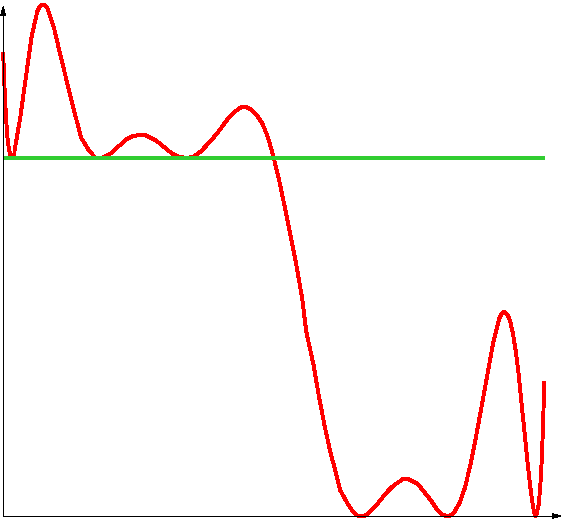
\includegraphics{Estieltjes_1.pdf}
   \caption{Graphe de $T$ pour $n=7$ et $k=4$}
   \label{fig:Estieltjes_1}
\end{figure}

\subsection*{Partie II}
Pour chaque entier $i$ entre $1$ et $n$ et différent de $k$, on définit un polynôme $\Lambda_i$  par :
\begin{displaymath}
\Lambda_i = (X-x_i)(X-x_k)\prod_{j\in\{1,\cdots,n\}-\{i,k\}}(X-x_j)^2
\end{displaymath}
\begin{enumerate}
\item Préciser pour tout couple $(i,j)$ d'entiers entre 1 et $n$ les valeurs de $\widetilde{L_i}(x_j)$.
\item Montrer que $(L_1,\cdots,L_n)$ est une base de $A$. Préciser les coordonnées d'un polynôme $P$ dans cette base.
\item Pour tout $i$ différent de $k$ entre $1$ et $n$, montrer que $\widetilde{\Lambda'_i}(x_i) \neq 0 $ et que
\begin{align*}
 \forall j\in \{1,\cdots ,n\} : \widetilde{\Lambda_i}(x_j)&=0 \\
 \forall j\in \{1,\cdots ,n\} \text{ tel que } j\neq i \text{ et } j\neq k: \widetilde{\Lambda'_i}(x_j)&=0
\end{align*}
\item \begin{enumerate}
\item Montrer que 
\begin{displaymath}
 \left( L_1,\cdots,L_n,\Lambda_1,\cdots,\Lambda_{k-1},\Lambda_{k+1},\cdots,\Lambda_n\right) 
\end{displaymath}
est une base de $E$.
\item Calculer les coordonnées de $T$ dans cette base.
\end{enumerate}
\item \begin{enumerate}
\item Montrer que $T'$ admet $2n-3$ racines distinctes et préciser leurs positions par rapport aux $x_i$.
\item {\'E}tudier les variations de $T$.
\item Montrer que :
\begin{align*}
\forall t \leq x_1 &: \widetilde{T}(t)\geq 1\\
\forall t \in \R &: \widetilde{T}(t)\geq 0 
\end{align*}
Que peut-on conclure pour le coefficient dominant de $T$ ?
\end{enumerate}
\end{enumerate} 
%
\newpage%
\part*{Corrigés} \addcontentsline{toc}{part}{Corrigés.} %
\section*{Problème 1}%
\addcontentsline{toc}{section}{Pb 1 : Borne inférieure et addition parallèle. }%
\fancyhead[LO,RE]{Corrigés - Pb 1 : Borne inférieure et addition parallèle. }%
\begin{enumerate}
\item L'addition parall{\`e}le est clairement commutative. L'associativit{\'e} se d{\'e}duit de ce que
\[(a//b)//c=\frac{\frac{ab}{a+b}c}{\frac{ab}{a+b}+c}=\frac{abc}{ab+ac+bc}\]
s'exprime de mani{\`e}re sym{\'e}trique en fonction de $a$, $b$, $c$.\newline 
Il n'existe pas de neutre car $a//b=b$ entrainerait $0=b^{2}$. La question des {\'e}l{\'e}ments inversibles ne se pose pas car il n'y a pas d'{\'e}l{\'e}ment neutre.

\item L'ensemble des $(y,z)\in \R^{2}$ tels que $y+z=x$ est aussi l'ensemble des $(y,x-y)$ o{\`u} $y$ est un r{\'e}el quelconque. \newline
Consid{\'e}rons la fonction du second degr{\'e} en $y$
$$ay^{2}+b(x-y)^{2}=(a+b)y^{2}-2bxy+bx^{2}$$
Comme $a+b>0$, la plus petite valeur que prend cette expression est atteinte pour $$y_0=\frac{bx}{a+b}$$ et vaut
\[\frac{b^{2}x^{2}}{a+b}-\frac{2b^{2}x^{2}}{a+b}+bx^{2}=\frac{ab}{a+b}x^{2}.\]
Ainsi, $(a//b)x^{2}$ est non seulement la borne inf{\'e}rieure mais aussi le plus petit {\'e}l{\'e}ment de l'ensemble propos{\'e}. La relation est v{\'e}rifi{\'e}e pour
\[(y_0,z_0)=(\frac{bx}{a+b},x-\frac{bx}{a+b}).\]

\item Avec les conventions de l'{\'e}nonc{\'e}, $ay^{2}$ et $bz^{2}$ repr{\'e}sentent les {\'e}nergies dissip{\'e}es dans chaque r{\'e}sistance. Le courant se r{\'e}partit entre les deux branches de fa\c{c}on {\`a} minimiser l'{\'e}nergie dissip{\'e}e. La r{\'e}sistance {\'e}quivalente $a//b$ permet d'exprimer cette {\'e}nergie en respectant la loi d'Ohm.

\item Consid{\'e}rons des r{\'e}els $y$ et $z$ quelconques tels que $y+z=x$. D'apr{\`e}s la question pr{\'e}c{\'e}dente :
\[(a//c)x^{2}+(b//d)x^{2}\leq ay^{2}+cz^{2}+by^{2}+dz^{2}=(a+b)y^{2}+(c+d)z^{2}\]
Donc $(a//c)x^{2}+(b//d)x^{2}$ est un minorant de
\[\{(a+b)y^{2}+(c+d)z^{2},(y,z)\in \R^{2}\,\mathrm{ tq }\,y+z=x\}.\]
Comme la borne inférieure $((a+b)//(c+d))$ est le plus grand des minorants, on a bien l'in{\'e}galit{\'e} propos{\'e}e.

\item Cette formule s'obtient de mani{\`e}re {\'e}vidente par r{\'e}currence {\`a} partir de la pr{\'e}c{\'e}dente.
\end{enumerate}
%
\newpage%
\section*{Problème 2}%
\addcontentsline{toc}{section}{Pb 2 : Algèbre linéaire dans un espace de polynômes.}%
\fancyhead[LO,RE]{Corrigés - Pb 2 : Algèbre linéaire dans un espace de polynômes.}%
\subsection*{Pr{\'e}liminaires}
\begin{enumerate}
 \item Comme $f^0$ est l'identité, son noyau $\{0_V\}$ est inclus dans $\ker f$. Pour $k\in \N^*$,
\begin{displaymath}
 \forall x\in V, \; x\in\ker f^k
\Rightarrow f^k(x)=0_V \Rightarrow f\left( f^k(x)\right) = f(0_V)=0_V
\Rightarrow x\in\ker f^{k+1}
\end{displaymath}
Ce qui montre la chaîne d'inclusions demandée.
\item Soit $p$ un entier tel que $\ker f^p = \ker f^{p+1}$, nous allons montrer que 
\begin{displaymath}
 \ker f^{p+2} \subset \ker f^{p+1}
\end{displaymath}
Cela entrainera que $\ker f^p = \ker f^{p+1} = \ker f^{p+2}$ à cause de l'inclusion  toujours valide $\ker f^{p+1} \subset \ker f^{p+2}$. On peut alors déduire par récurrence l'égalité de tous les noyaux suivants.\newline
Il s'agit donc de montrer que $\ker f^{p+2} \subset \ker f^{p+1}$.
Cela résulte de 
\begin{multline*}
 \forall x\in V, \; x\in \ker f^{p+2} : f^{p+1}(f(x))=0_V\Rightarrow f(x)\in \ker f^{p+1}=\ker f^{p} \\
\Rightarrow f^{p+1}(x)=f^p(\underset{\in \ker f^p}{\underbrace{f(x}}))=0_V 
\Rightarrow x\in \ker f^{p+1}
\end{multline*}
\item On suppose que $V$ est de dimension finie, tous les sous-espace de $V$ sont alors de dimension finie. La suite $\left( \dim \ker f^k \right) _{k\in \N}$ définit une fonction croissante de $\N$ dans l'ensemble fini $\llbracket 0, \dim V\rrbracket$. Une telle suite ne peut pas être strictement croissante car elle serait injective. Il existe donc des entiers $k$ tels que $\dim f^k < \dim f^{k+1}$ soit faux ce qui entraine $\dim f^k = \dim f^{k+1}$ car $\dim f^k \leq \dim f^{k+1}$. Soit $p$ le plus petit de ces $k$. Il vérifie
\begin{displaymath}
 0=\dim (\ker f^0) < \dim (\ker f^1)< \cdots<\dim (\ker f^p) = \dim (\ker f^{p+1}) \leq \dim V=n
\end{displaymath}
Comme les premières inégalités sont strictes et qu'il y en a $p$, on obtient
\begin{displaymath}
 p\leq \dim (\ker f^p) \leq n
\end{displaymath}
D'après un résultat de cours sur les sous-espaces en dimension finie:
\begin{displaymath}
 \left. 
\begin{aligned}
 \dim (\ker f^p) =& \dim (\ker f^{p+1}) \\
 \ker f^p \subset& \ker f^{p+1}
\end{aligned}
\right\rbrace 
\Rightarrow \ker f^p = \ker f^{p+1}
\end{displaymath}
L'égalité se propage alors (d'après 2.) à tous les $k\geq p$ parmi lesquels figure $n$ ce qui entraine $\ker f^n = \ker f^{n+1}$.
\item Dans cette question, l'endomorphisme $u$ est nilpotent. D'après la question précédente, la suite \og croissante\fg~ des $\ker u^k$ se stabilise avant $n$ à sa valeur finale qui est $V$ tout entier. On en déduit qu'il existe un $p\leq n$ tel que $V=\ker u^p$.\newline
On en tire que $V=\ker u^n$ c'est à dire que $u^n$ est l'endomorphisme nul.
\end{enumerate}

\subsection*{Partie I.}
\begin{enumerate}
  \item
     \begin{enumerate}
       \item La relation  $g_n^2=\lambda Id_{E_n} +D_n$ (entre des éléments de $\mathcal{L}(E_n)$) permet d'exprimer $D_n$ en fonction de $g_n$ :
\begin{displaymath}
 D_n=-\lambda Id_{E_n} + g_n^2
\end{displaymath}
Sous cette forme, il est {\'e}vident que $D_n$ commute avec $g_n$.\newline
Pour montrer qu'un sous-espace $E_p$ (avec $0\leq p \leq n$) est stable par $g$, on remarque que c'est un noyau. En effet: 
\begin{displaymath}
  E_p = \R_p[X] = \ker D_n^{p+1}
\end{displaymath}

Comme $g_n$ commute avec $D_n$, il commute aussi avec les puissance de $D_n$. En particulier
\begin{multline*}
 x\in E_p = \ker D_n^{p+1} \Rightarrow D_n^{p+1}(g_n(x))= g_n( D_n^{p+1}(x)) = g_n(0_{E_n}) = 0_{E_n}\\
 \Rightarrow g_n(x) \in \ker D_n^{p+1} = E_p
\end{multline*}
Une fois prouv{\'e}e la stabilit{\'e} de $E_p$ par $g_n$, on peut consid{\'e}rer la restriction $g_p$ de $g_n$ {\`a} $E_p$. Elle v{\'e}rifie {\'e}videmment la m{\^e}me relation que $g_n$.

 \item Le raisonnement est le m{\^e}me que pour la question pr{\'e}c{\'e}dente. Le fait que $E$ ne soit pas de dimension finie ne change rien. Si $g$ v{\'e}rifie la relation, il commute donc avec l'op{\'e}rateur de d{\'e}rivation.\newline
Comme plus haut, $E_n$ est stable par $g$ car c'est un noyau d'une puissance de $D_n$ et la restriction $g_n$ de $g$ v{\'e}rifie la m{\^e}me relation avec la restriction $D_n$ de $D$.
    \end{enumerate}
    
 \item
  \begin{enumerate}
 \item L'opérateur $D_F$ est la restriction {\`a} $F$ de l'op{\'e}rateur de d{\'e}rivation. Comme $F$ est de dimension finie, il existe un entier $k$ qui est le degr{\'e} maximal d'un polyn{\^o}me quelconque de $F$. Alors $D_F^{k+1}$ est nul.\newline
D'apr{\`e}s la partie pr{\'e}liminaire, comme $D_F$ est nilpotent dans un espace de dimension $n+1$, l'endomorphisme $D_F^{n+1}$ est nul. Ceci montre que $F\subset \R_n[X]$. Comme les deux espaces sont de m{\^e}me dimension, ils sont {\'e}gaux.\newline
On peut en conclure que les seuls sous-espaces de dimension finie stables par $D$ sont les $\R_n[X]$. \newline
Un seul sous-espace de dimension infinie est stable par $D$, il s'agit de $\R[X]$ lui m{\^e}me. En effet, un tel espace doit contenir des polyn{\^o}mes de degr{\'e} arbitrairement grand (sinon il serait de dimension finie) et tous leurs polynômes d{\'e}riv{\'e}s.

\item Soit $G$ un sous-espace de $E$. Supposons $G$ stable par $g$ et exploitons la relation fondamentale pour montrer que $G$ est stable par $D$.
\begin{displaymath}
\forall P \in G,\; D(P) = \underset{\in G}{\underbrace{g^2(P)}} - \underset{\in G}{\underbrace{\lambda P}} \in G 
\end{displaymath}
Réciproquement, supposons $G$ stable par $D$. D'après la question précédente (I.1.b) $G=\R[X]$ ou il existe $n\in \N$ tel que $G=E_n$.
\begin{itemize}
  \item Si $G=\R[X]$, il est évidemment stable par $g$.
  \item Si $G = E_n$, on a montré en I.1.b que $E_n = \ker D^{n+1}$ est stable par $g$.
\end{itemize}
          \end{enumerate}

  \item Cas $\lambda<0$.

\begin{enumerate}
       \item Dans $E_0=\R$ qui est un espace de dimension 1, les seules applications lin{\'e}aires sont les multiplications par un scalaire et $D_0$ est l'application nulle. S'il existe un $g_0$ (la multiplication par un $\mu\in \R$) vérifiant la relation, on peut écrire
\begin{displaymath}
  g_0^2 = \lambda {\Id}_{E_0} + D_0 \Leftrightarrow \mu^2=\lambda \Rightarrow \lambda \geq 0
\end{displaymath}
La condition nécessaire à l'existence d'un $g_0$ vérifiant la relation est donc $\lambda \geq 0$.

       \item D'apr{\`e}s 1.a., lorsqu'il existe un entier $n$ et un $g_n\in \mathcal{L}(E_n)$ vérifiant la relation, tous les sous-espaces $E_p$ avec $p \in      \llbracket 0,n \rrbracket$ sont stables par $g_n$. D'après 1.b., lorsqu'il existe un $g$ dans $\mathcal{L}(E)$ vérifiant la condition, tous les sous-espaces $E_p$ avec $p$ entier sont stables par $g$.\newline
       Dans les deux cas, $E_0$ est stable donc $\lambda \geq 0$. Ainsi, lorsque $\lambda<0$, il n'existe pas d'application $g$ v{\'e}rifiant la condition {\'e}tudi{\'e}e, ni dans $\mathcal{L}(E)$, ni dans un $\mathcal{L}(E_n)$.
     \end{enumerate}

  \item
     \begin{enumerate}
\item Soit $f$ lin{\'e}aire de $V$ dans $V$ telle que $f^{n+1}$ soit nulle mais pas $f^n$. Il existe alors un $y\in V$ tel que
\begin{displaymath}
f^n(y)\neq 0  
\end{displaymath}
Montrons que $\mathcal{B}=(y,f(y),\cdots,f^n(y))$ est libre.\newline
Si $(\lambda_{0},\lambda_{1},\cdots\lambda_{n})$ sont des r{\'e}els tels que
 \begin{displaymath}
\lambda_{0}y+\lambda_{1}f(y)+\cdots+\lambda_{n}f^n(y)=0   
 \end{displaymath}
en composant par $f^n$, on obtient $\lambda_{0}f^n(y)=0$ avec $f^n(y)\neq 0$ d'o{\`u} $\lambda_{0}=0$ et ainsi de suite. En composant successivement par $f^{n-1},f^{n-2},\cdots$ on obtient la nullit{\'e} de tous les coefficients. La famille est donc libre.\newline
Cette famille est une base car elle contient autant de vecteurs que la dimension de l'espace.
       
\item Dans le cas où l'endorphisme nilpotent est la dérivation restreinte à un espace $E_n = \R_n[X]$, 
\begin{displaymath}
  Y = X^n \Rightarrow \left( Y,D_n(Y),\cdots,D_n^n(Y)\right) 
\end{displaymath}
est une base de $E_n$. En fait n'importe quel polynôme de degré $n$ aurait fait l'affaire.
     \end{enumerate}

  \item Un exemple avec $n=2$ et $\lambda >0$.

\begin{enumerate}
  \item Il est bien {\'e}vident que les endomorphismes $h$ de la forme
\begin{displaymath}
  h = a \Id_{E_2} + bD_2 + c D_2^2
\end{displaymath}
commutent avec $D_2$. On va montrer que ce sont les seuls.\newline
Considérons $X^2\in \R_2[X]$, la famille $(X^2,D(X^2),D^2(X^2)) = (X^2,2X,2)$ est une base de $E_2$ d'après la question 4.b ou simplement car il s'agit d'une famille de 3 polynômes de degrés échelonnés dans $\R_2[X]$. Comme $f(X^2)\in E_2$, 
\begin{displaymath}
  \exists (a,b,c)\in \R^3 \text{ tel que } f(X^2) = aX^2 + bD(X^2) + cD^2(X^2)
\end{displaymath}
Définissons $F\in \mathcal{L}(E_2)$ par $F =a \Id_{E_2} + bD_2 + cD_2^2$ et comparons le à $f$. Pour cela, il suffit de les comparer sur les vecteurs d'une base (théorème du prolongement linéaire).\newline
Par d{\'e}finition de $F$:
\begin{align*}
 f(X^2)=& F(X^2) \\
f(D(X^2))=& D(f(X^2))=aD(X^2)+bD^2(X^2)=F(D(X^2)) \text{ car } D^3(X^2)=0 \\
f(D^2(X^2))=& D^2(f(X^2))=aD^2(X^2)=F(D^2(X^2))
\end{align*}
Les deux fonctions co{\"\i}ncident sur une base, elles sont donc {\'e}gales.

  \item Montrons que $\left( \Id_{E_2}, D_2, D_2^2\right)$ est une famille libre dans $\mathcal{L}(E_2)$. Considérons des réels $\alpha$, $\beta$, $\gamma$ tels que
\begin{displaymath}
  \alpha \Id_{E_2} + \beta D_2 + \gamma D_2^2 = 0_{\mathcal{L}(E_2)}
\end{displaymath}
et prenons la valeur de cette expression (endomorphis nul) successivement aux polynômes $1$, $X$ et $X^2$. On en tire dans l'ordre $\alpha = 0$, $\beta=0$, $\gamma =0$. La famille est donc bien libre.

  \item On doit chercher les $g_2$ telles que $g_2^2=\lambda \Id_{E_2} +D_2$ parmi les applications qui commutent avec $D_2$. Cherchons donc des conditions sur $a,b,c$ assurant que
\begin{displaymath}
g_2 = a\Id_{E_2} + bD_2 + cD_2^2  
\end{displaymath}
v{\'e}rifie $g_2^2=\lambda \Id_{E_2} + D_2$. Calculons $g^2$ :
\begin{displaymath}
g^2 = a^2 \Id_{E_2} + 2abD_2^2 + (b^2+2ac)D_2^2 = \lambda \Id_{E_2} + D_2  
\end{displaymath}
Comme $\left( \Id_{E_2}, D_2, D_2^2\right)$ est une famille libre, on peut identifier les coefficients. On trouve donc exactement deux endomorphismes répondant à la question, l'un étant déterminé par
\begin{displaymath}
a = \sqrt{\lambda},\hspace{0.5cm} b=\frac{1}{2\sqrt{\lambda}},\hspace{0.5cm} c=-\frac{1}{8\lambda \sqrt{\lambda}} 
\end{displaymath}
L'autre {\'e}tant son oppos{\'e}e.
     \end{enumerate}
\end{enumerate}

\subsection*{Partie II.}
\begin{enumerate}
  \item
\begin{enumerate}
\item On suppose ici $g_n^2 = D_n$. Comme $D_n$ est nilpotent $g_n$ l'est aussi. Si un endomorphisme $f$ est injectif, alors tous les $f^k$ le sont également,  par cons{\'e}quent $g_n^2$ et $g_n$ ne sont pas injectifs (une de leurs puissance est l'endomorphisme nul). Mais pourquoi $\ker g_n^2$ est-il de dimension au moins 2?\newline
Si ce n'était pas le cas, on aurait, avec $\ker g_n \subset \ker g_n^2$, 
\begin{displaymath}
  0 < \dim (\ker g_n) \leq \dim (\ker g_n^2) < 2 \Rightarrow \dim (\ker g_n) = \dim (\ker g_n^2) = 1 
\end{displaymath}
La suite des noyaux de $g_n^k$ est alors constante d{\`e}s le premier rang. Mais d'apr{\`e}s la partie pr{\'e}liminaire, sa valeur finale est $E_n$ autrement dit $g_n$ est nulle ce qui est absurde.
 \item Il n'existe pas de $g_n$ tel que $g_n^2 = D_n$ car le noyau de $D_n$ est de dimension 1 (polynômes constants) alors que celui de $g_n^2$ devrait {\^e}tre au moins 2.\newline
D'après la partie I, si $g^2 = D$, les espaces $E_n$ sont stables par $g$ et les restrictions $g_n$ vérifient $g_n^2 = D_n$ ce qui est impossible. 
     \end{enumerate}

  \item \begin{enumerate}
\item Tout polyn{\^o}me admet plusieurs polyn{\^o}mes \emph{primitifs} (c'est à dire dont le polynôme dérivé est égal au polynôme donné) qui diff{\`e}rent d'une constante. L'application $D$ et les applications $D^m$ sont donc surjectives.\newline 
La surjectivit{\'e} de $g^k$ entra{\^\i}ne celle de $g$ car $\Im g^k \subset \Im g$.

\item Pour $q\leq k$, $\ker g^q \subset \ker g^k=\ker D^m=E_{m-1}$ qui est de dimension finie $m$. On conclut avec le résultat de cours: tout sous-espace d'un espace de dimension finie est de dimension finie.

\item L'application $\Phi$ est lin{\'e}aire car c'est la restriction de $g$ à $\ker g^p$. Elle prend ses valeurs dans $\ker g^{q-1}$ car
\begin{displaymath}
  \forall x\in E, \; x\in \ker g^p \Rightarrow 0_E = g^p(x)=g^{p-1}(g(x)) \Rightarrow g(x)\in \ker g^{p-1}
\end{displaymath}
Montrons la surjectivit{\'e} de $\Phi$.\newline
Soit $x\in \ker g^{p-1}$. Comme $g$ est surjective, il existe un $y\in E$ tel que $x=g(y)$ et
\begin{displaymath}
0_E = g^{p-1}(x) = g^{p-1}(g(y)) = g^p(y)  
\end{displaymath}
donc $y\in \ker g^p$ et $y$ est un ant{\'e}c{\'e}dent par $\Phi$ de $x$.\newline
Ainsi $\Phi$ est surjective de $\ker g^p$ vers $\ker g^{p-1}$ de noyau $\ker g$. Le th{\'e}or{\`e}me du rang donne alors
\begin{displaymath}
\dim(\ker g^p) = \dim(\ker g^{p-1}) + \dim(\ker g)  
\end{displaymath}
La suite des dimensions est arithm{\'e}tique d'o{\`u}
\begin{displaymath}
\dim(\ker g^p)=p\dim(\ker g)
\end{displaymath}
     \end{enumerate}

  \item D'après la question précédente, comme $\dim(\ker D^m)=m$,
\begin{displaymath}
  g^k = D^m \Rightarrow
\dim (\ker g^k) = \dim (\ker D^m) \Rightarrow k\dim(\ker g) = m \Rightarrow k \text{ divise } m
\end{displaymath}
Réciproquement, si $k$ divise $m$, il existe $q\in \N$ tel que $m=qk$. En posant $g = D^q$, on vérifie
\begin{displaymath}
  g^k = D^{qk} = D^m
\end{displaymath}
La condition nécessaire et suffisante demandée est donc
\begin{displaymath}
  k \text{ divise } m
\end{displaymath}

\end{enumerate}

\subsection*{Partie III.}
\begin{enumerate}
  \item 
\begin{enumerate}
\item La fonction $\varphi$ est $\mathcal{C}^{\infty}$ dans $]-1,+\infty[$, elle admet donc, d'après la formule de Taylor avec reste de Young, des développements limités à tous les ordres.

\item \`A l'ordre $3$, le développement est usuel:
\begin{displaymath}
\varphi(x) = (1+x)^{\frac{1}{2}} = 1 + \frac{1}{2}x -\frac{1}{8}x^2 + \frac{1}{16}x^3 + o(x^3)  
\Rightarrow b_0=1, b_1=\frac{1}{2}, b_2=-\frac{1}{8}, b_3=\frac{1}{16}
\end{displaymath}
Pour $b_k$, on utilise l'expression venant de la formule de Taylor
\begin{displaymath}
b_k = \frac{\varphi^{(k)}(0)}{k!}
= \frac{1}{k!}\underset{k \text{ facteurs consécutifs}}{\underbrace{(\frac{1}{2})(\frac{1}{2}-1)(\frac{1}{2}-2) \cdots }}
= \frac{(-1)^{k-1}}{2^k\,k!}\prod_{i=1}^{k-1}(2i-1)
\end{displaymath}
Le produit étant constitué des impairs entre $1$ et $2k-3$. On le transforme
\begin{displaymath}
\prod_{i=1}^{k-1}(2i-1)
= \frac{(2k-2)!}{\text{pdt des pairs entre $2$ et $2k-2$}}
= \frac{(2k-2)!}{2^{k-1}(k-1)!}
\end{displaymath}
On en déduit
\begin{displaymath}
  b_k = \frac{(-1)^{k-1} (2k-2)!}{2^{2k-1}k!\,(k-1)!}
  = \frac{(-1)^{k-1} (2k-1)!}{2^{2k-1}(2k-1)k!\,(k-1)!}
  = \frac{(-1)^{k-1}}{2^{2k-1}(2k-1)}\binom{2k-1}{k}
\end{displaymath}

\item Pour montrer la formule demandée, il ne faut surtout pas chercher à combiner les coefficients du binôme mais utiliser le produit du développement limité par lui même. Pour tout $n$ entier, notons
\begin{displaymath}
a_m = \sum_{k=0}^{m}b_k\,b_{m-k}  
\end{displaymath}
En fait $a_m$ est le coefficient de $x^m$ dans le développement limité de $\varphi(x)^2 = 1+x$. On en déduit que $a_m=1$ pour $m=1$ ou $2$ et $a_n=0$ pour les autres valeurs.
\end{enumerate}

  \item On calcule $g_n^2$ en utilisant le fait que $\Id_{E_n}$ et $D_n$ commutent et que $D_n^{n+1}$ est l'endomorphisme nul:
\begin{displaymath}
g_n^2 = \sum_{(k,k')\in \llbracket 0,n \rrbracket^2} b_kb_k'D_n^{k+k'}  
\end{displaymath}
Pour $m$ entre $0$ et $2n$, on regroupe les $(k,k')$ tels que $k+k'=m$. En fait, seuls les $m \leq n$ contribuent significativement car $D_n^{n+1}$ est l'endomorphisme nul.\newline
Pour $m$ entre 0 et $n$, on retrouve les sommes $a_m$ de la question précédente
\begin{displaymath}
  g_n^2 = \sum_{m=0}^{n} a_m\,D_n^{m} = D_m^0 + D_m = \Id_{E_m} + D_m
\end{displaymath}

  \item On cherche à se rapprocher du cas précédent en factorisant par $\lambda$ lorsqu'il est non nul:
\begin{displaymath}
\lambda \Id_{E_n} + D_n = \lambda \left( \Id_{E_n} + \frac{1}{\lambda}D_n\right)   
\end{displaymath}
En remplaçant $D_n$ par $\frac{1}{\lambda}D_n$, un calcul analogue au précédent montre que 
\begin{displaymath}
\left( \sum_{k=0}^{n}\frac{b_k}{\lambda^{k}}D_n^k\right)^2 = \Id_{E_n} + \frac{1}{\lambda}D_n   
\end{displaymath}
Si $\lambda>0$, on peut poser
\begin{displaymath}
  g_n = \sqrt{\lambda}\left( \sum_{k=0}^{n}\frac{b_k}{\lambda^{k}}D_n^k\right)
\end{displaymath}
qui vérifie $g_n^2 = \lambda \Id_{E_m} + D_m$.\newline
L'expression suivant d'un endomorphisme de $E$ semble n'avoir aucun sens car elle fait intervenir une somme infinie
\begin{displaymath}
  g = \sqrt{\lambda}\left( \sum_{k=0}^{+\infty}\frac{b_k}{\lambda^{k}}D_n^k\right)
\end{displaymath}
En fait elle définit bien un endomorphisme car, pour chaque polynôme $P$, le calcul de $g(P)$ ne fait intervenir que les $k$ inférieurs ou égaux au degré de $P$. Si $n=\deg(P)$, tout se passe dans $E_n$ et $g(P)=g_n(P)$ d'où 
\begin{displaymath}
  g^2(P) = g_n^2(P) = \lambda P + D(P)
\end{displaymath}
Ceci étant valable pour tous les $P$, on a bien $g^2 = \lambda \Id_E + D$.
\end{enumerate}
%
\newpage%
\section*{Problème 3}%
\addcontentsline{toc}{section}{Pb 3 : Matrices de projecteurs.}%
\fancyhead[LO,RE]{Corrigés - Pb 3 : Matrices de projecteurs.}%
\begin{enumerate}
 \item On demande ici de montrer que certaines familles sont des bases et de préciser les matrices de passage à partir d'une base fixée.
Les vecteurs de ces familles (les $a_i$) sont donnés comme des combinaisons linéaires des vecteurs d'une base fixe (les $e_j$). Le plus économique est d'exprimer les $e_j$ en fonction des $a_i$. Cela montre que la famille des $a_i$ est génératrice (donc que c'est une base à cause du nombre d'éléments) et donne aussi la matrice de passage.\newline
Preuve que $\mathcal A$ est une base, calcul de $P_{\mathcal{A}\mathcal{E}}$. \newline
On transforme par opérations élémentaires le système de relations définissant $(a_1,a_2,a_3)$
\begin{displaymath}
\left\lbrace \begin{array}{lll}
a_1 &=& e_1 + e_2 + e_3 \\
a_2 &=& e_1  + e_3 \\
a_3 &=& -e_1 + e_2 + 2e_3 \\
\end{array} \right. 
\Leftrightarrow
\left\lbrace \begin{array}{lll}
e_1 &=& \frac{1}{3}a_1 + \frac{1}{3}a_2 -\frac{1}{3} a_3 \vspace{2pt}\\
e_2 &=& a_1  - a_2 \vspace{2pt}\\
e_3 &=& -\frac{1}{3}a_1 + \frac{2}{3}a_2 + \frac{1}{3}a_3 \vspace{2pt}\\
\end{array} \right. 
\end{displaymath}
On en déduit:
\begin{align*}
 P_{\mathcal E \mathcal A }=
\begin{pmatrix}
 1& 1 & -1 \\
1& 0 &1 \\
1 & 1 & 2
\end{pmatrix}
 &,& 
 P_{\mathcal A \mathcal E }= \frac{1}{3}
\begin{pmatrix}
 1& 3 & -1 \\
1& -3 & 2 \\
-1 & 0 & 1
\end{pmatrix}
\end{align*}
Preuve que $\mathcal A_1$ est une base, calcul de $P_{\mathcal A_1 \mathcal E}$.\newline
Exprimons $(e_1,e_2,e_3)$ en fonction de $(e_1,a_2,a_3)$
\begin{displaymath}
\left\lbrace \begin{aligned}
a_1 &= e_1 + e_2 + e_3 \\
a_2 &= e_1       + e_3 \\
a_3 &= -e_1 + e_2 + 2e_3 \\
\end{aligned} \right. 
\Rightarrow
\left\lbrace \begin{aligned}
e_1 &= e_1 \\
e_3 &= -e_1  + a_2 \\
e_2 &= e_1 + a_3 - 2e_3 \\
\end{aligned} \right.  
\Rightarrow
\left\lbrace \begin{aligned}
e_1 &= e_1 \\
e_2 &= 3e_1 - 2a_3 + a_3 \\
e_3 &= -e_1  + a_2 
\end{aligned} \right. 
\end{displaymath}
\begin{displaymath}
 P_{\mathcal A_1 \mathcal E} = 
\begin{pmatrix}
 1 & 3 & -1 \\
0 & -2 & 1 \\
0 & 1 & 0
\end{pmatrix} 
\end{displaymath}
Preuve que $\mathcal A_2$ est une base, calcul de $P_{\mathcal A_2 \mathcal E}$.\newline
Exprimons $(e_1,e_2,e_3)$ en fonction de $(a_1,e_2,a_3)$. On utilise l'expression des $e_j$ en fonction des $a_i$. De $e_2=a_1 - a_2$ on tire $a_2=a_1 -e_2$ que l'on remplace dans les deux autres relations. On obtient :
\begin{align*}
 \left\lbrace
\begin{array}{cc}
e_1 &= \frac{2}{3}a_1 -\frac{1}{3}e_2 -\frac{1}{3}a_3 \\
e_2 &= e_2 \\
e_3 &=  \frac{1}{3}a_1 -\frac{2}{3}e_2 +\frac{1}{3}a_3
\end{array}
 \right. 
&,&
 P_{\mathcal A_2 \mathcal E} = \frac{1}{3}
\begin{pmatrix}
 2 & 0 & \ 1 \\
- 1 & 3 & -2\\
-1 & 0 & 1
\end{pmatrix}
\end{align*}

\item On rappelle que $p_1$ est le projecteur sur $\Vect (e_2,e_3)$ parallélement à $\Vect (e_1)$.
\begin{itemize}
 \item Calcul de $\underset{\mathcal{E}}{\Mat}\, p_1$. 
Par définition :
\begin{displaymath}
 \underset{\mathcal{E}}{\Mat}\, p_1=
\begin{pmatrix}
0 & 0 & 0 \\
0 & 1 & 0 \\
0 & 0 & 1
\end{pmatrix}
\end{displaymath}

\item Calcul de $\underset{\mathcal{A}}{\Mat}\, p_1$. 
On utilise la formule de changement de base avec les matrices de passage déjà trouvées
\begin{displaymath}
 \underset{\mathcal{A}}{\Mat}\, p_1 =
 P_{\mathcal A \mathcal E}\underset{\mathcal{E}}{\Mat}\, p_1 P_{ \mathcal E \mathcal A}
\end{displaymath}
\begin{displaymath}
\underset{\mathcal{A}}{\Mat}\, p_1 =
\frac{1}{3}
\begin{pmatrix}
 1& 3 & -1 \\
1& -3 & 2 \\
-1 & 0 & 1
\end{pmatrix}
\begin{pmatrix}
0 & 0 & 0 \\
0 & 1 & 0 \\
0 & 0 & 1
\end{pmatrix}
\begin{pmatrix}
1 & 1 & -1 \\
1 & 0 & 1 \\
1 & 1 & 2
\end{pmatrix} 
=
\frac{1}{3}
\begin{pmatrix}
 2 & -1 & 1 \\
-1 & 2  & 1 \\
 1 & 1 & 2
\end{pmatrix}
\end{displaymath}

\item Calcul de $\underset{\mathcal{E A}}{\Mat}\, p_1$. Par définition, $p_1(e_1)=0$, $p_1(e_2)=e_2$, $p_1(e_3)=e_3$. On peut exprimer ces vecteurs dans $\mathcal
A$ avec les calculs déjà faits. On obtient
\begin{displaymath}
\underset{\mathcal{E A}}{\Mat}\, p_1 = 
\frac{1}{3}
\begin{pmatrix}
 0 & 3 & -1 \\
0 & -3  & 2 \\
 0 & 0 & 1
\end{pmatrix}
\end{displaymath}

\item Calcul de $\underset{\mathcal{A E}}{\Mat}\, p_1$. 
De $a_1= e_1+e_2+e_3$ on déduit $p_1(a_1)=e_2+e_3$. De même  les autres colonnes s'obtiennent directement à partir des expressions des $a_i$ en fonction des $e_j$.
\begin{displaymath}
\underset{\mathcal{A E}}{\Mat}\, p_1 = 
\begin{pmatrix}
 0 & 0 & 0 \\
1 & 0  & 1 \\
 1 & 1 & 2
\end{pmatrix}
\end{displaymath}
\end{itemize}

\item On rappelle que $p_2$ est le projecteur sur $\Vect (e_2,e_3)$ parallèlement à $\Vect (a_1)$.
\begin{itemize}
 \item Calcul de $\underset{\mathcal{E}}{\Mat}\, p_2$. \`A partir de la définition de $a_1 = e_1+e_2+e_3$, il vient $p_2(e_1)=-e_2 -e_3$. On en déduit
\begin{displaymath}
\underset{\mathcal{E}}{\Mat}\, p_2 = 
\begin{pmatrix}
 0 & 0 & 0 \\
-1 & 1  & 0 \\
 -1 & 0 & 1
\end{pmatrix}
\end{displaymath}

\item Calcul de $\underset{\mathcal{A}}{\Mat}\, p_2$. Il faut exprimer $a_1,a_2, a_3$ en fonction de $a_1, e_2, e_3$. En partant des définitions de $a_1,a_2, a_3$, on obtient :
\begin{displaymath}
 \left\lbrace
\begin{aligned}
a_1&=a_1\\
a_2 &= a_1 -e_2 \\
a_3 &= -a_1+2e_2+3e_3
\end{aligned}
 \right. \Rightarrow
 \left\lbrace
\begin{aligned}
p_2(a_1)&=0\\
p_2(a_2) &= -e_2 = -a_1 +a_2 \\
p_2(a_3) &= 2e_2+3e_3 = a_1 + a_3
\end{aligned}
 \right.
\end{displaymath}
\begin{displaymath}
\underset{\mathcal{A}}{\Mat}\, p_2 =
\begin{pmatrix}
 0 & -1 & 1 \\
0 & 1  & 0 \\
 0 & 0 & 1
\end{pmatrix}
\end{displaymath}

\item Calcul de $\underset{\mathcal{E A}}{\Mat}\, p_2$. On exprime $p_2(e_2)=e_2$ et $p_2(e3)=e_3$ dans $\mathcal A$. De plus,
\begin{displaymath}
e_1=a_1-e_2-e_3\Rightarrow p_2(e_1)=-e_2 -e_3 = -\frac{2}{3}a_1 +\frac{1}{3}a_2 -\frac{1}{3}a_3
\end{displaymath}
d'où
\begin{displaymath}
\underset{\mathcal{E A}}{\Mat}\, p_2 = \frac{1}{3}
\begin{pmatrix}
 -2 & 3 & -1 \\
1 & -3  & 2 \\
-1 & 0 & 1
\end{pmatrix}
\end{displaymath}

\item Calcul de $\underset{\mathcal{A}\mathcal{E}}{\Mat}\, p_2$. On exprime $a_1, a_2, a_3$ en fonction de $a_1,e_2, e_3$. On obtient :
\begin{displaymath}
\left\lbrace 
\begin{aligned}
 a_2 &= a_1 -e_2\\
 a_3 &=-a_1+2e_2+3e_3
\end{aligned}
\right. \Rightarrow
 \underset{\mathcal{A E}}{\Mat}\, p_2 =
\begin{pmatrix}
0 & 0 & 0 \\
0 & -1  & 2 \\
0 & 0 & 3
\end{pmatrix}
\end{displaymath}

\end{itemize}
\end{enumerate}
%
\newpage%
\section*{Problème 4}%
\addcontentsline{toc}{section}{Pb 4 : Une bonne base pour des endomorphismes de trace nulle.}%
\fancyhead[LO,RE]{Corrigés - Pb 4 : Une bonne base pour des endomorphismes de trace nulle.}%
\begin{enumerate}
 \item La famille $\mathcal B_{i,j}$ est génératrice car tous les vecteurs $b_k$ de la base $\mathcal B$ s'expriment facilement en fonction de $b'_k$ de $\mathcal B_{i,j}$.
\begin{align*}
 b_k = b'_k &\text{ si } k\neq i \\
 b_k = b'_i - b'_j &\text{ si } k=i
\end{align*}
Comme cette famile contient $n$ vecteurs dans un espace de dimension $n$ cela suffit à montrer que c'est une base.\newline
Pour exprimer les matrices de passage, on peut utiliser les matrices élémentaires $E_{u,v}$ dont tous les termes sont nuls sauf le terme $(u,v)$ qui vaut $1$. On obtient
\begin{align*}
 P_{\mathcal B \mathcal B_{i,j}} = I_n + E_{j,i} & &
P_{\mathcal B_{i,j} \mathcal B } = I_n - E_{j,i}
\end{align*}
\item Supposons que la matrice de $f$ dans une base $\mathcal B=(b_1,\cdots,b_n)$ soit diagonale avec
\begin{displaymath}
 \Mat_{\mathcal B}f = 
\begin{bmatrix}
 \lambda_1 &0 &\cdots & 0 \\
0& \lambda_2 & &\vdots \\
\vdots & & \ddots & 0\\
0 &\cdots &0 & \lambda_n
\end{bmatrix}
\end{displaymath}
Alors :
\begin{align*}
 &f(b'_k) = f(b_k)=\lambda_k b_k=\lambda_k b'_k &\text{ si } k\neq i \\
 &f(b'_k) = f(b_i) + f(b_j)=\lambda_ib_i +\lambda_jb_j
=\lambda_ib'_i+(\lambda_j - \lambda_i)b'_j &\text{ si } k=i
\end{align*}
On en déduit
\begin{displaymath}
 \Mat_{\mathcal B_{i,j}} f =
\begin{bmatrix}
 \lambda_1 &0 &\cdots & 0 \\
0& \lambda_2 & &\vdots \\
\vdots & & \ddots & 0\\
0 &\cdots &0 & \lambda_n
\end{bmatrix}
+ (\lambda_j - \lambda_i)E_{j,i}
\end{displaymath}

\item \begin{enumerate}
 \item Supposons que la matrice de $f$ soit diagonale pour \emph{toutes} les bases de $E$. Elle est alors diagonale dans une certaine base $\mathcal B$ ainsi que dans toutes les bases $\mathcal B_{i,j}$ que l'on peut former à partir de $\mathcal B$ comme dans la question 1. Cela entraine qu'il existe un $\lambda$ tel que  $\lambda_i=\lambda_j$ pour tous les $i$ et $j$ distincts. On a donc que toutes les composantes non diagonales $(\lambda_j - \lambda_i)E_{j,i}$ sont nulle. Tous les $\lambda_i$ sont égaux à un même $\lambda$ et
\begin{displaymath}
 f = \lambda Id_E
\end{displaymath}

\item D'après la question précédente, si $f\not \in \Vect (Id_E)$, il existe une base $\mathcal B$ de $E$ telle que $\Mat_{\mathcal B}f$ ne soit pas diagonale. Il existe donc deux entiers $i$ et $j$ distincts entre $1$ et $n$ tels que le terme $i,j$ de la matrice soit non nul ce qui entraine que $f(b_i)\not\in \Vect(b_i)$ ou encore $(b_i,f(b_i))$ libre.
\end{enumerate}

\item Avec les notations de l'énoncé :
\begin{displaymath}
 \Mat_{(u_2,u_3)} g =
\begin{bmatrix}
 b' & c' \\
b'' & c''
\end{bmatrix}
\end{displaymath}

\item \begin{enumerate}
 \item La trace d'un endomorphisme est par définition la trace de sa matrice dans n'importe quelle base. Cette définition a du sens car les matrices d'un endomorphisme dans n'importe quelle base ont toutes la même trace. En effet, on sait que 
\begin{displaymath}
 \tr (AB) = \tr (BA)
\end{displaymath}
pour toutes matrices carrées $A$ et $B$ dans $\mathcal M_n(\R)$. On utilise alors la formule de changement de base :
\begin{displaymath}
 \Mat_{\mathcal B'} f = P_{\mathcal B \mathcal B'}^{-1} \Mat_\mathcal B f P_{\mathcal B \mathcal B'}
\end{displaymath}
On en déduit 
\begin{displaymath}
\tr\left(  \Mat_{\mathcal B'} f\right)  = \tr \left( P_{\mathcal B \mathcal B'}^{-1} \Mat_\mathcal B f P_{\mathcal B \mathcal B'}\right) 
=\tr\left(\Mat_\mathcal B f P_{\mathcal B \mathcal B'} P_{\mathcal B \mathcal B'}^{-1}\right) 
=\tr\left(\Mat_\mathcal B f \right) 
\end{displaymath}

\item La matrice d'un endomorphisme $\lambda Id_E$ est, dans n'importe quelle base, diagonale avec des $\lambda$ sur la diagonale. Sa trace est $\dim E\, \lambda$. Le seul élément de $\Vect(Id_E)$ dont la trace est nulle est donc l'endomorphisme nul. 

\item Ici $f$ est un endomorphisme de trace nulle d'un espace $E$ de dimension 2. Comme $f$ n'est pas dans $\Vect(Id_E)$, d'après la question 3.b., il existe un $x$ de $E$ tel que $(x,f(x))$ est libre. \`A cause de la dimension cette famille est une base de $E$. La matrice de $f$ dans cette base est de la forme
\begin{displaymath}
 \begin{bmatrix}
  0 & \alpha \\
 1 & \beta
 \end{bmatrix}
\end{displaymath}
Cette matrice est de trace nulle donc $\beta=0$. Pour cette base, tous les termes diagonaux de la matrice de $f$ sont donc nuls.

\item La situation est analogue à celle de la question précédente mais $E$ est de dimension $3$. D'après la question 3.b., il existe un $x$ de $E$ tel que $(x,f(x))$ est libre. En utilisant le théorème de la base incomplète, on forme une base de $E$
\begin{displaymath}
 (x,f(x),y)
\end{displaymath}
Dans cette base, la matrice de $f$ est de la forme
\begin{displaymath}
 \begin{bmatrix}
  0 & b & c \\
 1 & b' & c' \\
 0 & b'' & c''
 \end{bmatrix}
\end{displaymath}
Elle est de trace nulle donc $b'+c''=0$.\newline
Considérons un endomorphisme $g$ comme dans la question 4. L'endomorphisme $g$ est la restriction à $\Vect(f(x),y)$ de $p\circ f$ où $p$ est la projection sur $\Vect(f(x),y)$ parallèlement à $\Vect(x)$. Alors
\begin{displaymath}
 \Mat_{(f(x),y)}g = 
\begin{bmatrix}
 b' & c' \\
 b'' & c''
\end{bmatrix}
\end{displaymath}
donc $g$ est un endomorphisme de $\Vect(f(x),y)$ de trace nulle. D'après la question 5.c., il existe une base $(v,w)$ de $\Vect(f(x),y)$ telle que :
\begin{displaymath}
 \Mat_{(v,w)}g = 
\begin{bmatrix}
 0 & \beta \\
 \alpha & 0
\end{bmatrix}
\end{displaymath}
Remarquons que $f(x)$ et $y$ s'expriment en fonction de $v$ et $w$ car $(v,w)$ est une base de $\Vect(f(x),y)$. On en déduit que $(x,u,v)$ est génératrice donc que c'est une base. De plus, la matrice de $f$ dans cette base est de la forme
\begin{displaymath}
 \begin{bmatrix}
  0 & C & D \\
 A & 0 & \beta \\
 B & \alpha & 0
 \end{bmatrix}
\end{displaymath}
Bien noter que les éléments non nuls de la première ligne et de la première colonne ont changé.
\end{enumerate}
\end{enumerate}
%
\newpage%
\section*{Problème 5}%
\addcontentsline{toc}{section}{Pb 5 : Calculs matriciels}%
\fancyhead[LO,RE]{Corrigés - Pb 5 : Calculs matriciels}%
\begin{enumerate}
\item \begin{enumerate}
\item  En utilisant les op\'{e}rations $L_{4}\leftarrow L_{4}-\alpha L_{1}$ et $L_{2}\leftarrow L_{2}-2L_{1}$, le rang de $A$ est aussi celui de 
\begin{displaymath}
\begin{pmatrix}
1 & 1 & 0 & 0 \\
0 & -1 & 1 & 1 \\ 
0 & 0 & 0 & \alpha  \\ 
0 & 0 & 0 & 0
\end{pmatrix}
 \end{displaymath}
On en d\'{e}duit que le rang est 2 si $\alpha =0$, le rang est 3 sinon.
\item  Pour d\'{e}terminer une base de l'image, on cherche 2 ou 3 colonnes combinaisons des colonnes de $A$ et les engendrant.
Pour la base du noyau, on cherche des combinaisons nulles de colonnes de $A$. On obtient :

\begin{itemize}
\item  si $\alpha =0$ : $\Im f=\Vect(e_{1},e_{2})$, $\ker f=\Vect(e_{3}-e_{4},e_{1}-e_{2}-e_{3}).$

\item  si $\alpha \neq 0$ : $\Im f=\Vect(e_{2},e_{3},e_{1}+\alpha e_{4})$, $\ker f=\Vect(e_{1}-e_{2}-e_{3})$.
\end{itemize}

\item Pour toutes les valeurs du réel  $\alpha$, l'image et le noyau de $f$ sont suppl\'{e}mentaires. En effet, dans les deux cas, la somme des dimensions est $4$. Il suffit donc de vérifier que l'intersection est réduite au vecteur nul. Pour cela, examinons l'image d'un vecteur de l'image.
\begin{itemize}
 \item Dans le cas $\alpha=0$. 
\begin{displaymath}
 \begin{pmatrix}
  1 & 1 & 0 & 0 \\ 2 & 1 & 1 & 1 \\ 0 & 0 & 0 & 0\\ 0 & 0 & 0 & 0 
 \end{pmatrix}
\begin{pmatrix}
 \lambda \\ \mu \\ 0 \\ 0
\end{pmatrix}
=
\begin{pmatrix}
  \lambda + \mu \\ 2\lambda + \mu \\ 0 \\ 0
\end{pmatrix}
=
\begin{pmatrix}
 0 \\ 0 \\ 0 \\ 0
\end{pmatrix}
\Rightarrow
\left\lbrace 
\begin{aligned}
 \lambda + \mu &= 0 \\ 2\lambda + \mu &= 0 
\end{aligned}
\right. 
\Rightarrow \lambda = \mu = 0
\end{displaymath}

 \item Dans le cas $\alpha \neq 0$. 
\begin{multline*}
 \begin{pmatrix}
  1 & 1 & 0 & 0 \\ 2 & 1 & 1 & 1 \\ 0 & 0 & 0 & \alpha\\ \alpha & \alpha & 0 & 0 
 \end{pmatrix}
\begin{pmatrix}
 x_1 \\ x_2 \\ x_3 \\ \alpha x_1
\end{pmatrix}
=
\begin{pmatrix}
  x_1+x_2 \\ (2+\alpha) x_1 + x_2 +x_3 \\ \alpha^2 x_1 \\ \alpha(x_1+x_3)
\end{pmatrix}
=
\begin{pmatrix}
 0 \\ 0 \\ 0 \\ 0
\end{pmatrix} \\
\Rightarrow x_1 = x_2 = x_3 = 0
\end{multline*}
\end{itemize}
Un autre moyen simple de montrer que les espaces sont supplémentaires serait de former des famille en concaténant les bases obtenues pour le noyau et l'image chaque cas puis de calculer le rang de la matrice de ces familles. On trouverait facilement $4$ ce qui montrerait que ce sont des bases et donc que les espaces sont supplémentaires.
\end{enumerate}

\item  D'après la base de $\Im f$ trouvée à la question précédente lorsque $\alpha\neq 0$, on peut choisir $\lambda =1$ soit $\varepsilon _{1}=e_{1}+\alpha e_{4}$, $\varepsilon _{2}=e_{2}$, $\varepsilon_{3}=e_{3}$.\newline
En fait on \emph{doit} choisir $\lambda=1$ car, si $e_1+\alpha e_4 \in \Im f$, il existe des réels $u$, $v$, $w$ tels que
\begin{displaymath}
 e_1+\alpha e_4 = ue_2 + v e_3 +w(e_1+\alpha e_4) \Rightarrow
\left\lbrace 
\begin{aligned}
 \lambda &= w & &\text{ coeff. de } e_1\\
 \alpha &= w\alpha & &\text{ coeff. de } e_4
\end{aligned}
\right. \Rightarrow w = \lambda = 1
\end{displaymath}

\item L'application $g$ est lin\'{e}aire par d\'{e}finition, elle prend ses valeurs dans $F=\Im f$ puisque c'est une restriction de $f$.
D'autre part :
\begin{eqnarray*}
g(\varepsilon _{1})&=&e_{1}+2e_{2}+\alpha e_{4}+\alpha (e_{2}+\alpha
e_{3})=e_{1}+\alpha e_{4}+(2+\alpha )e_{2}+\alpha ^{2}e_{3}\\
&=&\varepsilon_{1}+(2+\alpha )\varepsilon _{2}+\alpha ^{2}\varepsilon _{3}\\
g(\varepsilon _{2})&=&e_{1}+e_{2}+\alpha e_{4}=\varepsilon _{1}+\varepsilon
_{2}\\ 
g(\varepsilon _{3})&=&e_{2}=\varepsilon _{2}
\end{eqnarray*}
\[\mathop{\mathrm{Mat}}_{\mathcal B}\,g  =\left( 
\begin{array}{ccc}
1 & 1 & 0 \\ 
2+\alpha  & 1 & 1 \\ 
\alpha ^{2} & 0 & 0
\end{array}
\right) \]

\item  L'application $g$ est inversible car c'est la restriction de $f$ \`{a} un suppl\'{e}mentaire de son noyau. Le calcul de la matrice inverse
conduit \`{a} 
\begin{displaymath}
\mathop{\mathrm{Mat}}_{\mathcal B}\,g^{-1}=\frac{1}{\alpha ^{2}}\left( 
\begin{array}{ccc}
0 & 0 & 1 \\ 
\alpha ^{2} & 0 & -1 \\ 
-\alpha ^{2} & \alpha ^{2} & -(\alpha +1)
\end{array}
\right)  
\end{displaymath}


\item 
\begin{enumerate}
\item Les conditions de l'\'{e}nonc\'{e} d\'{e}finissent $h$ dans $F$ par prolongement linéaire en précisant les images d'une base de $F$. Comme $\ker f$ et $F=\Im f$ sont suppl\'{e}mentaires, poser $h(x)=0$ pour $x$ dans $\ker f$ comme l'impose l'énoncé achève de définir $h$ dans $E$. Il prend évidemment ses valeurs dans $E$, c'est donc bien un endomorphisme.\newline
\'Ecrivons d'abord la matrice de $h$ dans $\mathcal{B}^{\prime }=(\varepsilon_{1}, \varepsilon_{2}, \varepsilon_{3},\varepsilon_{4})$ avec $\varepsilon_{4}=e_{1}-e_{2}-e_{3}$. Comme $(\varepsilon_{4})$ est une base de $\ker f$, on a : 
\[
\mathop{\mathrm{Mat}}_{\mathcal B'}\,h=\frac{1}{\alpha ^{2}}\left( 
\begin{array}{cccc}
0 & 0 & 1 & 0 \\ 
\alpha ^{2} & 0 & -1 & 0 \\ 
\alpha ^{2} & \alpha ^{2} & -(\alpha +1) & 0 \\ 
0 & 0 & 0 & 0
\end{array}
\right) 
\]
Utilisons ensuite la formule de changement de base $$\mathop{\mathrm{Mat}}_{\mathcal C}\,h=P^{-1}\mathop{\mathrm{Mat}}_{\mathcal B'}\,h\cdot P$$
avec $P=P_{\mathcal{B}^{\prime }C}$. D'autre part: 
\begin{displaymath}
\left\{ \begin{aligned}
\varepsilon _{1} &=  e_{1}+\alpha e_{4} \\ 
\varepsilon _{2} &=  e_{2} \\ 
\varepsilon _{3} &=  e_{3} \\ 
\varepsilon _{4} &=  e_{1}-e_{2}-e_{3}
\end{aligned}
\right. \Rightarrow \left\{ 
\begin{aligned}
e_{1} &=  \varepsilon _{2}+\varepsilon _{3}+\varepsilon _{4} \\ 
e_{2} &= \varepsilon _{2} \\ 
e_{3} &= \varepsilon _{3} \\ 
e_{4} &= \frac{1}{\alpha }(\varepsilon _{1}-\varepsilon _{2}-\varepsilon_{3}-\varepsilon _{4})
\end{aligned}
\right. 
\end{displaymath}

\[
P^{-1}=\left( 
\begin{array}{cccc}
1 & 0 & 0 & 1 \\ 
0 & 1 & 0 & -1 \\ 
0 & 0 & 1 & -1 \\ 
\alpha  & 0 & 0 & 0
\end{array}
\right) \quad \quad P=\left( 
\begin{array}{cccc}
0 & 0 & 0 & \frac{1}{\alpha } \\ 
1 & 1 & 0 & -\frac{1}{\alpha } \\ 
1 & 0 & 1 & -\frac{1}{\alpha } \\ 
1 & 0 & 0 & -\frac{1}{\alpha }
\end{array}
\right) 
\]
\[
D=\mathop{\mathrm{Mat}}_{\mathcal C}\,h=\frac{1}{\alpha ^{3}}
\begin{pmatrix}
\alpha                    & 0        & \alpha            & -1 \\ 
-\alpha                   & 0        & -\alpha           & \alpha ^{2}+1 \\ 
\alpha^3-\alpha^2 -\alpha & \alpha^3 & -\alpha^2 -\alpha & -2\alpha ^{2}+\alpha +1 \\ 
\alpha^2                  & 0        & \alpha^2          & -\alpha
\end{pmatrix}
\]

\item Il ne faut surtout pas calculer le produit matriciel. Remarquons plut\^{o}t que $ADA$ est la matrice dans $\mathcal{B}$ de $f\circ h\circ f$.
Dans $\ker f$, l'endomorphisme $f\circ h\circ f$ est toujours nul; dans $%
\Im f$, $h\circ f=h\circ g=Id_{\Im f}$ donc $f\circ h\circ f$
co\"{i}ncide avec $f$. Comme $\ker f$ et $\Im f$ sont
suppl\'{e}mentaires et que $f\circ h\circ f$ et $f$ co\"{i}ncident sur ces
sous-espaces, ils sont \'{e}gaux dans $E$ tout entier. On en d\'{e}duit $%
ADA=A$.
\end{enumerate}
\end{enumerate}
%
\newpage%
\section*{Problème 6}%
\addcontentsline{toc}{section}{Pb 6 : Exercice d'algèbre linéaire matricielle.}%
\fancyhead[LO,RE]{Corrigés - Pb 6 : Exercice d'algèbre linéaire matricielle.}%
\begin{enumerate}
 \item On trouve
\begin{displaymath}
 A^2=
\begin{pmatrix}
 1&-1&1&-1\\0&0&0&0\\2&-2&2&-1\\2&-2&2&-1
\end{pmatrix}
\hspace{0.5cm}
(A-I_4)^2=
\begin{pmatrix}
 0&1&-3&3\\0&1&-2&2\\0&0&1&-1\\0&0&0&0
\end{pmatrix}
\hspace{0.5cm}
A^2(A-I_4)^2=0_{\mathcal M_4(\R)}
\end{displaymath}

 \item
\begin{enumerate}
 \item Comme $A^2=\mathop{\mathrm{Mat}}_{\mathcal A} f^2$ et $(A-I_4)^2=\mathop{\mathrm{Mat}}_{\mathcal A}(f-\mathrm{id}_E)^2$, la formule du rang donne $\dim N_1 = 4 -\rg A^2 = 2$ et $\dim N_2 = 4 -\rg (A-I_4)^2 = 2$ car les deux rangs sont égaux à $2$.\newline
Ces rangs sont calculés en transformant les matrices par opérations élémentaires.
\begin{itemize}
 \item On transforme $A^2$ par les opérations $L_4\leftarrow L_4 - L_3$, $L_3\leftarrow L_3 - 2L_1$. Le rang est donc le même que celui de
\begin{displaymath}
\begin{pmatrix}
 1&-1&1&-1\\0&0&0&0\\0&0&0&1\\0&0&0&0
\end{pmatrix}
\hspace{0.3cm} \text{qui est clairement $2$.}
\end{displaymath}

\item  On transforme $(A-I_4)^2$ par les opérations $L_1\leftarrow L_1 +3 L_3$, $L_2\leftarrow L_2 + 2L_1$, $L_2\leftarrow L_2 -L_1$. Le rang est donc le même que celui de
\begin{displaymath}
\begin{pmatrix}
 0&1&0&0\\0&0&0&0\\0&0&1&-1\\0&0&0&0
\end{pmatrix}
\hspace{0.3cm} \text{qui est clairement $2$.}
\end{displaymath}
\end{itemize}
Comme $N_1$ et $N_2$ sont deux sous-espaces de dimension $2$ d'un espace de dimension $4$, il suffit de montrer que leur intersection est réduite au vecteur nul pour prouver qu'ils sont supplémentaires.\newline
 Un vecteur $v$ de coordonnées $(x,y,z,t)$ est dans cette intersection si et seulement si $(x,y,z,t)$ est solution d'un système linéaire de $8$ équations. Certaines de ces équations sont triviales ($0=0$) ou équivalentes. Avec \emph{les mêmes opérations sur les lignes} qui ont servi à calculer le rang, elles se ramènent à :
\begin{displaymath}
 v\in N_1\cap N_2 \Leftrightarrow
\left\lbrace 
\begin{aligned}
 &x - &y + &z - &t &=0\\
 &\phantom{x} &\phantom{y} &\phantom{z} &t &= 0\\
 &\phantom{x} &y &\phantom{z} &\phantom{t} &= 0\\
 &\phantom{x} &\phantom{y} &z -&t &=0
\end{aligned}
\right.
\Leftrightarrow
\left\lbrace 
\begin{aligned}
 x &=0\\
 y &= 0\\
 z &= 0\\
 t &=0
\end{aligned}
\right.
\end{displaymath}
On pouvait aussi raisonner vectoriellement. Si $x$ est dans les deux noyaux alors 
\begin{displaymath}
 \left\lbrace
\begin{aligned}
f^2(x)-2f(x)+x&=0_E\\
f^2(x)&=0_E 
\end{aligned}
\right.
\Rightarrow
 \left\lbrace
\begin{aligned}
f(x)&= \frac{1}{2}x\\
f^2(x)&=0_E 
\end{aligned}
\right.
 \Rightarrow
0_E=f^2(x)=\frac{1}{4}x
 \Rightarrow x=0_E .
\end{displaymath}

 \item Si $v\in N_1$ alors $f^2(f(v))=f(f^2(v))=f(0_E)=0_E$ donc $f(v)\in N_1$. Le sous-espace $N_1$ est stable par $f$. \newline
De même, si $v\in N_2$ alors $(f-\mathrm{id}_E)^2(f(v))=f((f-\mathrm{id}_E)^2(v))=f(0_E)=0_E$ donc $f(v)\in N_2$. Le sous-espace $N_2$ est stable par $f$. Le point important ici est que $f$ commute avec les endomorphismes dont on considère le noyau.
\end{enumerate}

 \item
\begin{enumerate}
 \item On a montré à la question 1 que $A^2(A-I_4)^2$ est la matrice nulle. Cela entraine que $f^2\circ (f-\mathrm{id}_E)^2$ et  $(f-\mathrm{id}_E)^2\circ f^2$ sont égaux à l'endomorphisme nul donc que $\Im (f^2)\subset N_1$ et $\Im((f-\mathrm{id}_E)^2)\subset N_1$. Par le calcul de rang déjà fait, les deux images sont de dimension $2$. De l'égalité des dimensions, on déduit l'égalité des sous-espaces.  
 \item Le vecteur $u_2$ doit vérifier $f(u_2)=u_1$ et $f^2(u_2)=f(u_1)=0_E$. Il s'agit donc d'un vecteur de $N_1$ qui n'est pas dans dans le noyau de $f$. On trouve de tels vecteurs en considérant les colonnes de $(A-I_4)^2$. La première ne convient pas car elle correspond à un élément du noyau, en combinant les colonnes 2 et 3 on peut former $u_2=-e_1+e_3$ puis $u_1=f(u_2)=e_1+e_2$.\newline
Choisissons un vecteur $u_4$ dans $N_2$, par exemple $u_4=e_1$ qui est dans $N_2$ car la première colonne de $(A-I_4)^2$ est nulle. Posons $u_3=(f-\mathrm{id}_E)(u_4)=e_3+e_4$. On a alors $u_3 = f(u_4)-u_4$ donc $f(u_4)=u_3+u_4$. De plus, de $(f-\mathrm{id}_E)^2(u_4)=0_E$, on tire alors $f(u_3)=u_3$.\newline
On vérifie facilement que la famille $\mathcal{U}=(e_1+e_2,-e_1+e_3,e_3+e_4,e_1)$ est une base. Par construction de ces vecteurs :
\begin{displaymath}
 \mathop{\mathrm{Mat}}_{\mathcal U}f=
\begin{pmatrix}
 0&1&0&0\\0&0&0&0\\0&0&1&1\\0&0&0&1
\end{pmatrix}
\end{displaymath}

\end{enumerate}

\end{enumerate}
%
\newpage%
\section*{Problème 7}%
\addcontentsline{toc}{section}{Pb 7 : Exemples d'espaces supplémentaires.}%
\fancyhead[LO,RE]{Corrigés - Pb 7 : Exemples d'espaces supplémentaires.}%
\begin{enumerate}
 \item
\begin{enumerate}
 \item Commençons par signaler que l'espace vectoriel contenant $\ker g $ et $\Im f$ est $F$. Il s'agit donc de $0_F$ dans la formule proposée.
\begin{itemize}
 \item Supposons $\ker g\circ f \subset \ker f$. Soit $x$ quelconque dans $\ker g \,\cap\, \Im f$. Il existe $a\in E$ tel que $x=f(a)$. Comme $x\in \ker g$, on a aussi
\begin{displaymath}
 g(x)=O_G \Rightarrow g\circ f(a) =0_G \Rightarrow a\in \ker g\circ f \subset \ker f
\Rightarrow x=f(a)=0_F
\end{displaymath}
Ainsi, $\ker g \,\cap\, \Im f=\{0_F\}$.
\item Supposons $\ker g \,\cap\, \Im f=\{0_F\}$. Soit $x$ quelconque dans $\ker g \circ f$. Alors $g\circ f(x)=0_G$ donc $f(x)\in \ker g$. Or évidemment $f(x)\in \Im f$ donc $f(x)\in \ker g \,\cap \Im f = \left\lbrace 0_F\right\rbrace $ c'est à dire $x\in \ker f$.\newline
Ainsi $\ker g \circ f \subset \ker f$.
\end{itemize}

 \item
\begin{itemize}
 \item Supposons $\Im g \subset \Im g\circ f$. Soit $x$ quelconque dans $F$, considérons $g(x)$. Il appartient à $\Im g$ qui est inclus dans $\Im g\circ f$, il existe donc $a\in E$ tel que $g(x)=g\circ f(a)$. On peut alors écrire
\begin{displaymath}
 x = f(a) + (x-f(a))
\end{displaymath}
avec $f(a)\in \Im f$ et $g(x-f(a))=g(x)-g\circ f(a)=0_G$ donc $x-f(a)\in \ker g$.\newline
Ainsi $F=\Im f + \ker g$.
 \item Supposons $F=\Im f + \ker g$. Soit $u$ quelconque dans $\Im g$. Il existe $x\in F$ tel que $u=g(x)$. D'après l'hypothèse, ce $x$ se décompose. Il existe $a\in E$ et $y\in \ker g$ tels que
\begin{displaymath}
 x= f(a)+y
\end{displaymath}
En composant par $g$, on obtient
\begin{displaymath}
 u=g(x) = g(f(a)) + \underset{=0_G}{\underbrace{g(y)}} = g\circ f(a) \in \Im g\circ f
\end{displaymath}
Ainsi $\Im g \subset \Im g\circ f$.
\end{itemize}
\end{enumerate}
 
 \item
\begin{enumerate}
 \item On cherche à utiliser la question 1. qui permet de caractériser le fait que le noyau et l'image sont supplémentaires. On forme des conséquences des relations de l'énoncé permettant de le faire:
\begin{displaymath}
 \left. 
\begin{aligned}
 f\circ g \circ f &= f \\ g\circ f \circ g &= g 
\end{aligned}
\right\rbrace 
\Rightarrow
\left\lbrace 
\begin{aligned}
 \ker g\circ f &\subset \ker f \\ \Im g &\subset \Im g\circ f
\end{aligned}
\right. 
\end{displaymath}
On peut donc appliquer la question 1. (avec $G=E$) et en déduire que $\ker g$ et $\Im f$ sont supplémentaires.\newline
L'autre propriété s'obtient en échangeant les rôles de $f$ et $g$.
 \item Pour tout $x\in \Im f$, il existe $a\in E$ tel que $x=f(a)$. Par définition de $\overline{f}$ et $\overline{g}$ on a alors:
\begin{displaymath}
 \overline{f}\circ\overline{g}(x) = \overline{f}\circ\overline{g}(f(a))
= \overline{f}(g(f(a))) = f\circ g \circ f (a) = f(a)=x
\end{displaymath}
On en déduit $\overline{f}\circ\overline{g} =\Id_{\Im f}$. On montre de même que $\overline{g}\circ\overline{f} =\Id_{\Im g}$.\newline
Comme $\Im g$ est un supplémentaire de $\ker f$, le lemme noyau-image du cours assure directement que $\overline{f}$ est un isomorphisme. Cela s'applique aussi pour $\overline{g}$. On prouve bien ainsi qu'il s'agit d'isomorphismes mais pas qu'ils sont inverses l'un de l'autre.
\end{enumerate}

 \item
\begin{enumerate}
 \item Ici $g\circ f = \Id_E$. Alors $\ker g\circ f =\{0_E\}\subset \ker f$ et $\Im g\circ f =E$ donc $\Im g \subset \Im g\circ f$. On en déduit, d'après 1 avec $E=F=G$ que $\ker g$ et $\Im f$ sont supplémentaires.\newline
Cette question n'est intéressante que si on ne suppose pas la dimension finie. En effet $g\circ f = \Id_E$ entraine $g$ surjective et $f$ injective. Si on était en dimension finie, les deux seraient bijectifs donc vérifiant $\ker g =\{0_E\}$ et $\Im f = E$.\newline
En revanche, ces sous-espaces peuvent ne pas être triviaux en dimension finie comme le montre l'exemple demandé dans la question suivante.
 
 \item On définit $f$ par $f(P)=XP$ et $g$ par $g(P)$ est le quotient de la division de $P$ par $X$. On a alors immédiatement
\begin{displaymath}
 g\circ f =\Id_{\R[X]}
\end{displaymath}
Comme $g(1)=0$, $f\circ g (1)=0$ donc $f\circ g$ n'est pas l'identité. Quel que soit l'exemple choisi, $g\circ f = \Id_E$ entraine $\ker f = \{0_E\}$ et $\Im g = E$.
\end{enumerate}
\end{enumerate}
%
\newpage%
\section*{Problème 8}%
\addcontentsline{toc}{section}{Pb 8 : Du paramétrique au cartésien: éliminer.}%
\fancyhead[LO,RE]{Corrigés - Pb 8 : Du paramétrique au cartésien: éliminer.}%
\begin{enumerate}
 \item Le vecteur $x$ appartient à $\Vect(u_1,u_2,u_3)$ si et seulement si il existe des réels $\lambda_1$, $\lambda_2$, $\lambda_3$ tels que $x=\lambda_1u_1+\lambda_2u_2+\lambda_3u_3$. Cela est équivalent à \emph{l'existence} d'une solution pour le système suivant de $4$ équations à $3$ inconnues $\lambda_1$, $\lambda_2$, $\lambda_3$.
\begin{displaymath}
 (S):\left\lbrace 
\begin{aligned}
 \lambda_1  &+ 3\lambda_2 &- \lambda_3   &= x_1\\
 \lambda_1  &             &+ 2\lambda_3 &= x_2\\
 \lambda_1  &+ 5\lambda_2 &- 3\lambda_3 &= x_3\\
 2\lambda_1 &+  \lambda_2 &+ 3\lambda_3 &= x_4
\end{aligned}
\right. 
\end{displaymath}
On transforme ce système en des systèmes équivalents par des opérations élémentaires
\begin{displaymath}
 (S)\Leftrightarrow\left\lbrace 
\begin{aligned}
 \lambda_2  &+ 2\lambda_1 &+ 3\lambda_3 &= x_4\\
            &+   \lambda_1 &+ 2\lambda_3 &= x_2\\
            &- 5\lambda_1 &- 10\lambda_3 &= x_1-3x_4\\
            &- 9\lambda_1 &- 18\lambda_3 &= x_3-5x_4
\end{aligned}
\right.
\Leftrightarrow\left\lbrace 
\begin{aligned}
 \lambda_2  &+ 2\lambda_1 &+ 3\lambda_3 &= x_4\\
            &+  \lambda_1 &+ 2\lambda_3 &= x_2\\
            &             &         0   &= x_1-3x_4+5x_2\\
            &             &         0   &= x_3-5x_4+9x_2
\end{aligned}
\right. 
\end{displaymath}
On en déduit que $x \in \Vect(u_1,u_2,u_3)$ si et seulement si
\begin{displaymath}
 \left\lbrace 
\begin{aligned}
 0   &= x_1-3x_4+5x_2\\
 0   &= x_3-5x_4+9x_2
\end{aligned}
\right. 
\end{displaymath}
Il existe plusieurs systèmes d'équations possibles pour ce sous-espace. Si vous en avez un autre, pour le valider, vérifier que les vecteurs suivants sont solutions
\[
 (3,0,5,1) \hspace{1cm} (-5,1,-9,0).
\]

 \item Avec les notations précédentes $x_i = \alpha_i(x)$. On peut donc choisir
\begin{displaymath}
 \left\lbrace 
\begin{aligned}
 \alpha   &= \alpha_1 - 3\alpha_4 + 5\alpha_2\\
 \beta   &= \alpha_3 - 5\alpha_4 + 9\alpha_2
\end{aligned}
\right. 
\end{displaymath}
Pourquoi $(\alpha,\beta)$ est-elle libre ? Si $\lambda\alpha +\mu\beta$ est la forme nulle, la valeur en $a_1$ donne $\lambda=0$ et la valeur en $a_3$ donne $\mu=0$.  
\end{enumerate}
%
\newpage%
\section*{Problème 9}%
\addcontentsline{toc}{section}{Pb 9 : Algèbre linéaire et relation de récurrence linéaire d'ordre 3.}%
\fancyhead[LO,RE]{Corrigés - Pb 9 : Algèbre linéaire et relation de récurrence linéaire d'ordre 3.}%
\begin{enumerate}
 \item \begin{enumerate}
 \item La relation de récurrence étant linéaire, il est immédiat que si $(x_n)_{n\in\N}$ et $(y_n)_{n\in\N}$ sont dans $E_a$ et $\lambda$ et $\mu$ dans $\R$, la suite $(\lambda x_n + \mu y_n)_{n\in\N} \in E_a$.
\item Chaque suite dans $E_a$ est définie de manière unique par ses trois premiers termes et la relation de  récurrence. L'application
\begin{displaymath}
 \fonc{\phi}{E_a}{\R^3}{(x_n)_{n\in\N}}{(x_0,x_1,x_2)}
\end{displaymath}
est un isomorphisme linéaire. La dimension de $E_a$ est donc $3$.
\end{enumerate}
\item \begin{enumerate}
 \item On vérifie (simplement en remplaçant dans la relation de récurrence) que les fonctions constantes sont dans $E_a$.
\item La suite $(v_n)_{n\in\N}$ est définie par la différence entre deux termes consécutifs. En \og cassant\fg~ les coefficients $(1+a)$ et $(1+4a)$ de la relation $(1)$, celle-ci s'écrit
\begin{align*}
 4(u_{n+3}-u_{n+2}) &= 4a(u_{n+2}-u_{n+1}) -(u_{n+1}-u_n) \\
4v_{n+2} &= 4a v_{n+1}-v_n
\end{align*}
La suite $(v_n)_{n\in\N}$ vérifie donc
\begin{align*}
 4v_{n+2}-4av_{n+1}+v_n= 0 \hspace{2cm}(2)
\end{align*}
\item On désigne par $F_a$ l'ensemble des suites vérifiant $(2)$. Montrons d'abord qu'une suite vérifiant $(2)$ vérifie aussi $(1)$.\newline
Soit $(x_n)_{n\in\N}\in F_a$, d'après $(2)$ on a :
\[
 x_n = 4ax_{n+1}-4x_{n+2} 
 \Rightarrow x_{n+1} = 4a x_{n+2} - 4x_{n+3}
 \Rightarrow 4ax_{n+2}-x_{n+1} = 4x_{n+3}.
\]
En remplaçant dans le membre de droite de $(1)$, on a:
\begin{multline*}
4(1+a)x_{n+2}-(1+4a)x_{n+1}+x_n \\ 
= 4ax_{n+2}-x_{n+1}+ \underset{= -x_n \text{ d'après (2)}}{\underbrace{4x_{n+2}-4ax_{n+1}}} + x_n  
= 4ax_{n+2}-x_{n+1} = 4x_{n+3}.
\end{multline*}
Ceci prouve que $(x_n)_{n\in\N} \in E_a$ d'où $F_a\subset E_a$. Cet ensemble $F_a$ est stable par combinaison linéaire comme tout ensemble de suites vérifiant une relation de récurrence linéaire. On en conclut que $F_a$ est un sous-espace vectoriel de $E_a$.

La relation $(2)$ est vérifiée par les suites fabriquées à partir de celles de $E_a$ en prenant la différence de deux termes consécutifs. Mais les suites de $F_a$ sont elles toutes de cette forme ? \newline
En fait oui. L'application qui a une suite associe la différence de deux termes consécutifs est un endomorphisme de $E_a$ dont l'image est \emph{incluse} dans $F_a$ qui est de dimension $2$. Le noyau de cette application linéaire est $K$ (espace des suites constantes) qui est de dimension $1$. Le rang est donc $2$ ce qui prouve que $F_a$ est \emph{l'image} de l'application.
\end{enumerate}
\item Pour déterminer une base de $F_a$, on forme l'équation caractéristique
\begin{displaymath}
4x^2-4ax+1=0 
\end{displaymath}
dont le discriminant est $16(a^2-1)$.\newline
Lorsque $0\leq a <1$, l'équation a deux racines complexes conjuguées. On pose $a=\cos \theta$ avec $\theta \in ]0,\frac{\pi}{2}[$. Les racines sont $\frac{1}{2}e^{i\theta}$ et $\frac{1}{2}e^{-i\theta}$. Une base est alors (cours) :
\begin{displaymath}
 ((2^{-n}\cos n\theta)_{n\in\N},(2^{-n}\sin n\theta)_{n\in\N})
\end{displaymath}
Lorsque $a=1$. L'équation a une racine double $\frac{1}{2}$.  Une base est alors (cours) :
\begin{displaymath}
 ((2^{-n})_{n\in\N},(2^{-n} n)_{n\in\N})
\end{displaymath}
Lorsque $1<a$, l'équation a deux racines réelles. On pose $a=\ch \theta$ avec $\theta >0$. Les racines sont $\frac{1}{2}e^{\theta}$ et $\frac{1}{2}e^{-\theta}$. Une base est alors (cours) :
\begin{displaymath}
 ((2^{-n}e^{n\theta})_{n\in\N},(2^{-n}e^{-n\theta})_{n\in\N})
\end{displaymath}

\item L'ensemble $K$ des suites constantes est dans $F_a$ si et seulement si la suite constante de valeur $1$ est dans $E_a$ c'est à dire
\begin{align*}
 \forall k\in \N &: 4 = 4(1+a)-(1+4a)+1
\end{align*}
Ce qui ne se produit que pour
\begin{displaymath}
 a_0 = \dfrac{5}{4}
\end{displaymath}
\item Dans cette question, on suppose $a\neq\frac{5}{4}$.
\begin{enumerate}
 \item 
L'hypothèse $a\neq\frac{5}{4}$ entraîne que $K$ n'est pas inclus dans $F_a$. Comme c'est une droite vectorielle, on en tire $K\cap F_a=\{(0)\}$. Ici $(0)$ désigne la suite nulle. De plus :
\begin{itemize}
 \item $K$ est de dimension $1$ (la famille constituée de la suite constante de valeur $1$ en est une base) 
\item $F_a$ est de dimension $2$ (question 3.)
\item  $E_a$ est de dimension $3$  (question 1.b.)
\end{itemize}
Il en résulte que $K$ et $F_a$ sont supplémentaires dans $E_a$.\newline 
Soit $\left( u_n\right) _{n\in \N}$ une suite quelconque de $E_a$. Comment se décompose-t-elle sur ces deux supplémentaires?\newline
Elle est la somme d'une suite constante de valeur $c$ et d'une suite $\left( v_n\right) _{n\in \N}$ de $F_a$. Cette dernière suite est caractérisée par ses deux premiers termes $v_0$ et $v_1$. Pour calculer $c$, $v_0$, $v_1$, formons les relations venant des trois premiers termes
\begin{displaymath}
\left\lbrace  
\begin{aligned}
 c + v_0 &= u_0 & &\times\frac{1}{4}\\
 c + v_1 &= u_1 & &\times(-a)\\
 c -\frac{1}{4} v_0 + av_1 &= u_2 & &\times 1
\end{aligned}
\right. 
\end{displaymath}
et combinons les pour trouver $c$. En sommant avec les coefficients indiqués, on obtient
\begin{displaymath}
  c=\frac{\frac{1}{4}u_0-au_1+u_2}{\frac{5}{4}-a},\hspace{0.5cm} v_0=u_0 -c,\hspace{0.5cm} v_1=u_1 -c
\end{displaymath}

\item On obtient des bases de $E_a$ simplement en insérant $(1)$ (la suite constante de valeur $1$) dans les familles trouvées en 3.
\end{enumerate}
\item Dans le cas particulier $a_0=\frac{5}{4}$ la relation de récurrence définissant $E_{a_0}$ devient 
\begin{displaymath}
 4x_{n+3}=9x_{n+2}-6x_{n+1}+x_n
\end{displaymath}
Elle est vérifiée par $(n)_{n\in\N}$. Les racines de l'équation caractéristique (de $F_a$) sont alors $1$ et $\frac{1}{4}$. En fait 1 est une racine double de l'équation caractéristique de degré 3 de $E_a$. Bien que ce ne soit pas vraiment plus compliqué que pour les récurrences d'ordre 2, les récurrences linéaires d'ordre 3 ou plus ne sont pas au programme.
Pour montrer que la famille
\begin{displaymath}
 ((n)_{n\in\N},(1)_{n\in\N},(4^{-n})_{n\in\N})
\end{displaymath}
est une base de $E_{a_0}$, il suffit (dimension) de prouver qu'elle est libre. Supposons donc que
\begin{displaymath}
 \alpha(n)_{n\in\N} +\beta(1)_{n\in\N}+\gamma(4^{-n})_{n\in\N})=(0)
\end{displaymath}
\'Ecrivons la nullité des trois premiers termes et transformons le système par opérations élémentaires :
\begin{multline*}
% use packages: array
\renewcommand{\arraystretch}{2}
\left\lbrace \begin{array}{lclclcl}
& & \beta &+& \gamma & = & 0\\ 
\alpha &+&\beta &+& \dfrac{1}{4}\gamma &= & 0 \\ 
2\alpha &+&\beta &+& \dfrac{1}{16}\gamma &= &0
\end{array}\right. 
\Leftrightarrow
\left\lbrace \begin{array}{lclclcl}
\alpha &+&\beta &+& \dfrac{1}{4}\gamma &= & 0 \\ 
& & \beta &+& \gamma & = & 0\\ 
 & -&\beta  &+& -\dfrac{7}{16}\gamma &= &0
\end{array}\right. 
\\ \Leftrightarrow
\left\lbrace \begin{array}{lclclcl}
\alpha &+&\beta &+& \dfrac{1}{4}\gamma &= & 0 \\ 
& & \beta &+& \gamma & = & 0\\ 
 & &  &+& (1-\dfrac{7}{16})\gamma &= &0
\end{array}\right. 
\end{multline*}
ce qui entraîne $\alpha = \beta = \gamma$ et donc que la famille est libre.

\item Une suite de $E_a$ se décompose comme une somme d'une suite constante et d'une suite de $F_a$. La question 5.a. donne la valeur $c$ de la suite constante de cette décomposition. On trouve ici $c=1$ avec les conditions initiales particulières. Notons $\left( v_n\right) _{n\in \N}$ la composante dans $F_a$. Elle admet pour conditions initiales
\begin{displaymath}
 v_0=-\sqrt{|a^2-1|},\hspace{0.5cm} v_1 = 0,\hspace{0.5cm} v_2 = \frac{1}{4}\sqrt{|a^2-1|}
\end{displaymath}
Lorsque $a=1$, cette suite est identiquement nulle donc $u_n=1$ pour tous les $n$.\newline
Lorsque $a=\cos \theta\in [0,1[$ les conditions initiales deviennent
\begin{displaymath}
 v_0=-\sin \theta,\hspace{0.5cm} v_1 = 0,\hspace{0.5cm} v_2 = \frac{1}{4}\sin \theta
\end{displaymath}
Comme la suite est dans $F_a$, il existe $\lambda$ et $\mu$ tels que 
\begin{displaymath}
 \forall n\in \N,\hspace{0.5cm}v_n = \lambda 2^{-n}\cos(n\theta) + \mu2^{-n}\sin(n\theta)
\end{displaymath}
Les conditions initiales conduisent à
\begin{displaymath}
 \left\lbrace 
\begin{aligned}
\lambda &= -\sin \theta\\
\frac{\cos \theta}{2}\lambda + \frac{\sin \theta}{2}\mu &=0 
\end{aligned}
\right. 
\Rightarrow
 \left\lbrace 
\begin{aligned}
\lambda &= -\sin \theta\\
\mu &= \cos \theta 
\end{aligned}
\right. 
\end{displaymath}
On en déduit
\begin{displaymath}
 \forall n\in \N,\hspace{0.5cm}v_n = 2^{-n}\sin((n-1)\theta),\hspace{0.5cm} u_n= 1 +2^{-n}\sin((n-1)\theta)
\end{displaymath}
Dans le cas $a=\ch\theta >1$, des calculs analogues conduisent à 
\begin{displaymath}
 \forall n\in \N,\hspace{0.5cm}v_n = 2^{-n}\sh((n-1)\theta),\hspace{0.5cm} u_n= 1 +2^{-n}\sh((n-1)\theta)
\end{displaymath}

\end{enumerate}%
\newpage%
\section*{Problème 10}%
\addcontentsline{toc}{section}{Pb 10 : Approximation de pi, accélération de convergence.}%
\fancyhead[LO,RE]{Corrigés - Pb 10 : Approximation de pi, accélération de convergence.}%
\begin{enumerate}
 \item 
\begin{enumerate}
 \item On montre facilement par récurrence que la suite des $c_n$ est bien définie et que $0<c_n<1$ pour tout $n\geq 1$. Il existe donc des $\theta_n \in ]0 ,\frac{\pi}{2}[$ tels que $c_n=\cos \theta_n$. On définit $\alpha_n$ par $\alpha_n = \frac{\lambda_n}{\sin \theta_n}$.
 \item On peut calculer explicitement les $\theta_n$. En effet $c_1=0$ donc $\theta_1=\frac{\pi}{2}$ et $c_2=\frac{1}{\sqrt{2}}$ donc $\theta_2=\frac{\pi}{4}$. D'autre part,
\begin{displaymath}
 c_{n+1}=\sqrt{\frac{1+\cos \theta_n}{2}} = \cos \frac{\theta_n}{2}\Rightarrow \theta_{n+1}=\frac{\theta_n}{2}
\end{displaymath}
On en tire
\begin{displaymath}
 \theta_n = \frac{\pi}{2^n}
\end{displaymath}
Par définition, $\alpha_1=\frac{2}{\sin \theta_1}=2$ et
\begin{displaymath}
 \frac{\alpha_{n+1}}{\alpha_n} = \frac{\lambda_{n+1} \sin\theta_n}{\lambda_n \sin\theta_{n+1}}
=\frac{\sin \theta_n}{\cos \theta_{n+1}\sin \theta_{n+1}} =2
\end{displaymath}
On en déduit $\alpha_n = 2^n$ et $\lambda_n = 2^n \sin \frac{\pi}{2^n}$ converge vers $\pi$ car $\sin x$ est équivalent à $x$ en $0$.
\end{enumerate}

 \item Appliquons la formule de Taylor-Lagrange à la fonction $\sin$ entre $0$ et $a$ et à l'ordre $3$. Il existe $b\in[0,a]$ tel que
\begin{displaymath}
 \sin a = a -\frac{a^3}{3!} \cos(b)
\end{displaymath}
car $\sin^{(3)}=-\cos$. En particulier, pour $a=\frac{\pi}{2^n}$, on en tire
\begin{displaymath}
 \left| \sin \frac{\pi}{2^n} - \frac{\pi}{2^n}\right|\leq \frac{\pi^3}{6\times 2^{3n}}
\Rightarrow
 \left| \lambda_n - \pi\right| \leq \frac{\pi^3}{6\times 4^{n}}
\end{displaymath}
en multipliant par $2^n$.
 
 \item \'Ecrivons la formule de Taylor-Young pour le $\sin$ en $0$ à l'ordre $2p+1$.
\begin{displaymath}
 \sin x = x -\frac{1}{3!}x^3 + \cdots + (-1)^p\frac{1}{(2p+1)!}x^{2p+1} + o(x^{2p+1})
\end{displaymath}
 En substituant $\frac{\pi}{2^n}$ (qui tend vers $0$ quand $n$ tend vers l'infini) à $x$ et en multipliant par $2^n$, on obtient la formule demandée.

 \item Accélération de convergence.
\begin{enumerate}
 \item On peut combiner linéairement les développements précédents:
\begin{align*}
 \lambda_n    &= \pi &-& \frac{\pi^3}{6}\,\frac{1}{4^n}         & &+& \frac{\pi^5}{5!}\,\frac{1}{4^{2n}}
  &  &+& o(\frac{1}{4^{2n}}) & &\times -1\\  
\lambda_{n+1} &= \pi &-& \frac{\pi^3}{6}\,\frac{1}{4^n\times 4} & &+& \frac{\pi^5}{5!}\,\frac{1}{4^{2n}\times 16}
  &  &+& o(\frac{1}{4^{2n}}) & &\times 4 
\end{align*}
 On en déduit
\begin{multline*}
 3\lambda_n^{(1)}= 3\pi
-\frac{\pi^3}{6}\,\frac{1}{4^n}\left(-1+\frac{4}{4} \right)
+\frac{\pi^5}{5!}\,\frac{1}{4^{2n}}\left(-1 +\frac{4}{16}\right) \frac{1}{4^{2n}}+o(\frac{1}{4^{2n}})\\\Rightarrow
\lambda_n^{(1)} = \pi -\frac{\pi^5}{5!\times 4}\,\frac{1}{4^{2n}} +o(\frac{1}{4^{2n}})
\Rightarrow 
\lambda_n^{(1)} - \pi \sim -\frac{\pi^5}{5!\times 4 \times 4^{2n}}
\end{multline*}
Comme $\lambda_n - \pi \sim -\frac{\pi^3}{6\times 4^n}$, on a bien $\lambda_n^{(1)} - \pi$ négligeable devant $\lambda_n - \pi$.

 \item  \'Ecrivons l'équivalence précédente comme une limite finie:
\begin{displaymath}
 \frac{\lambda_n^{(1)}}{-\frac{\pi^5}{5!\times 4^{2n+1}}} \rightarrow 1
\end{displaymath}
Pour $n+1$ mais avec le même dénominateur, cela donne
\end{enumerate}
\begin{displaymath}
 \frac{\lambda_{n+1}^{(1)}}{-\frac{\pi^5}{5!\times 4^{2n+1}}} \rightarrow \frac{1}{16}
\end{displaymath}
En multipliant la première relation par $\alpha$ et la deuxième par $1-\alpha$, la limite est alors
\begin{displaymath}
 \frac{15\alpha +1}{16}
\end{displaymath}
Si on choisit $\alpha = -\frac{1}{15}$ ce qui entraine
\begin{displaymath}
 \lambda_n^{(2)}=\frac{1}{15}\left( -\lambda_n^{(1)} +16\lambda_{n+1}^{(1)}\right) 
=\frac{1}{45}\left(\lambda_n -20 \lambda_{n+1} +64 \lambda_{n+2}\right) 
\end{displaymath}
On a bien
\begin{displaymath}
 \frac{\lambda_n^{(2)}}{-\frac{\pi^5}{5!\times 4^{2n+1}}} \rightarrow 0
\end{displaymath}
ce qui entraine $\lambda_n^{(1)} - \pi$ négligeable devant $\lambda_n - \pi$.
\end{enumerate}%
\newpage%
\section*{Problème 11}%
\addcontentsline{toc}{section}{Pb 11 : Expression intégrale de la limite des suites arithmético-géométriques.}%
\fancyhead[LO,RE]{Corrigés - Pb 11 : Expression intégrale de la limite des suites arithmético-géométriques.}%
\subsection*{Partie I. \'Etude de $\Phi$.}
\begin{enumerate}
\item  Pour chaque $t$ de $\left[ 0,\frac{\pi }{2}\right] $ la fonction $x\rightarrow \frac{1}{\sqrt{1-x^{2}\sin ^{2}t}}$ est croissante donc $x<y$
entra\^{i}ne
\begin{displaymath}
\forall t\in \left[ 0,\frac{\pi }{2}\right] ,\quad \frac{1}{\sqrt{1-x^{2}\sin ^{2}t}}\leq \frac{1}{\sqrt{1-y^{2}\sin ^{2}t}}  
\end{displaymath}
puis $\phi (x)\leq \phi (y)$. La fonction est donc croissante.

  \item En linéarisant : $\sin^2 t = \frac{1}{2} - \frac{1}{2}\cos(2t)$. La partie en $\cos 2t$ s'intègre en $\sin(2t)$ dont la contribution est nulle en $0$ et $\frac{\pi}{2}$. On en déduit
\begin{displaymath}
  \int_0^{\frac{\pi}{2}}\sin^2 t\,dt = \frac{\pi}{4}
\end{displaymath}
On aurait aussi pu remarquer, par le changement de variable $\frac{\pi}{2}-t$ que l'intégrale est égale à celle en $\cos$ et que la somme des deux vaut $\frac{\pi}{2}$.
  \item
\begin{enumerate}
  \item On applique l'inégalité des accroissements finis en remarquant que la dérivée 
\begin{displaymath}
  \varphi'(t) = \frac{1}{2}(1-t)^{-\frac{3}{2}}
\end{displaymath}
est positive et croissante dans $[0,A]$.
  \item Si $x$ et $y$ sont dans $[0,A]$ alors $x^2\sin^2 t$ et $y^2\sin^2 t$ sont aussi dans $[0,A]$ (car $0 <A<1$). On en déduit, par positivité de l'intégrale:
\begin{multline*}
  \left|\Phi(y) - \Phi(x)\right| \leq
\frac{(1-A)^{-\frac{3}{2}}}{2}\int_{0}^{\frac{\pi}{2}}\left| x^2\sin^2 t - y^2 \sin^2 t\right|\, dt \\
= \frac{(1-A)^{-\frac{3}{2}}}{2}|x^2-y^2|\int_{0}^{\frac{\pi}{2}}\sin^2t \,dt 
= \frac{(1-A)^{-\frac{3}{2}}}{2}|x-y|\underset{\leq 2}{\underbrace{(x+y)}}\frac{\pi}{4}
\end{multline*}
\end{enumerate}

  \item La formule précédente montre que \emph{la restriction} de $\Phi$ à $[0,A]$ est lipschitzienne donc continue. Pour chaque $x\in [0,1[$, il existe un $A<1$ tel que $x\in [0,A]$. Cela prouve bien que $\Phi$ est continue en $x$. Pour autant, cela \emph{ne prouve pas} que $\Phi$ soit lipschitzienne (ni même uniformément continue) dans $[0,1[$.
\end{enumerate}


\subsection*{Partie II. Changement de variable dans une intégrale}
\begin{enumerate}
\item 
\begin{enumerate}
\item  Le calcul de la dérivée de $v$ conduit à :
\begin{displaymath}
  v'(t) = \frac{(1+x)\cos t}{(1+x\sin^2t)^2}(1-x\sin^2t) \geq 0
\end{displaymath}
Cette fonction est donc strictement croissante, à valeurs entre $v(0)=0$ et $v(\frac{\pi}{2})=1$. On en déduit (définition de $\arcsin$) que $u$ est bien définie et à valeurs dans $[0,\frac{\pi}{2}]$.

\item La fonction $\arcsin$ est continue dans $[-1,1]$ et $\mathcal{C}^{\infty}$ dans $]-1,1[$. On en tire par composition que $u$ est continue dans $[0,\frac{\pi}{2}]$ et $\mathcal{C}^1$ dans $[0,\frac{\pi}{2}[$ seulement.\newline
Pour montrer la dérivabilité et la continuité de la dérivée en $\frac{\pi}{2}$, on doit utiliser le théorème de la limite de la dérivée. En d\'{e}rivant $\sin u(t)$ dans $\left[ 0,\frac{\pi }{2}\right[ $ on obtient
\begin{displaymath}
u^{\prime }(t)\cos u(t)=\frac{(1+x)(1-x\sin ^{2}t)\cos t}{(1+x\sin ^{2}t)^{2}} \hspace{1cm}(1)
\end{displaymath}
En $\frac{\pi }{2}$, $u(t)\rightarrow u(1)=\arcsin \frac{\pi}{2}=1$. Le second membre de (1) est \'{e}quivalent \`{a}
\begin{displaymath}
\frac{1-x}{1+x}\cos t\sim \frac{1-x}{1+x}(\frac{\pi }{2}-t)
\end{displaymath}
D'autre part,
\begin{align*}
\cos u(t)  =& \sqrt{1-\sin ^{2}u(t)}=\sqrt{1-\frac{(1+x)^{2}\sin ^{2}t}{(1+x\sin ^{2}t)^{2}}}\\
=& \sqrt{\frac{(\sin t-1)(x\sin t-1)(1+x\sin^{2}t+(1+x)\sin t)}{(1+x\sin ^{2}t)^{2}}} \\
\cos u(t) \sim &\sqrt{-\frac{(x-1)2(1+x)}{(1+x)^{2}}}\sqrt{-\sin t+1}\sim 
\sqrt{2\frac{1-x}{1+x}}\frac{\frac{\pi }{2}-t}{\sqrt{2}}
\end{align*}
On en d\'{e}duit finalement que $u^{\prime }(t)\rightarrow \sqrt{\frac{1-x}{1+x}}$ quand $t\rightarrow \frac{\pi }{2}$ ce qui prouve \`{a} la fois la d\'{e}rivabilit\'{e} de $u$ en $\frac{\pi }{2}$ avec $u^{\prime }(\frac{\pi }{2})=\sqrt{\frac{1-x}{1+x}}$ et la continuit\'{e} de la d\'{e}riv\'{e}e en ce point.

Par d\'{e}finition, $u(t)\in \left[ 0,\frac{\pi }{2}\right] $ donc $\cos u(t)>0$. L'\'{e}quation (1) montre alors que $u^{\prime }(t)>0$ lorsque $t\in \left[ 0,\frac{\pi }{2}\right[ $. On en d\'{e}duit qu'elle est strictement croissante dans $\left[ 0,\frac{\pi }{2}\right]$. Comme de plus $u(0)=0$ et $u(\frac{\pi }{2})=\frac{\pi }{2}$. C'est une bijection continue de $\left[ 0,\frac{\pi }{2}\right] $ dans $\left[ 0,\frac{\pi }{2}\right]$.

La bijection r\'{e}ciproque d'une bijection continue sur un intervalle est continue. La formule (1) montre que $u^{\prime }(t)$ ne s'annule pas dans $\left[ 0,\frac{\pi }{2}\right[ $ et 
\begin{displaymath}
 u^{\prime }(\frac{\pi }{2})=\sqrt{\frac{1-x}{1+x}}\neq 0
\end{displaymath}
La bijection r\'{e}ciproque de $u$ est donc d\'{e}rivable dans $\left[ 0,\frac{\pi }{2}\right] $. L'expression 
\begin{displaymath}
(u^{-1})'=\frac{1}{u^{\prime }\circ u^{-1}} 
\end{displaymath}
de la d\'{e}riv\'{e}e montre sa continuit\'{e}.

\item Comme $\arcsin$ est à valeurs entre $-\frac{\pi}{2}$ et $\frac{\pi}{2}$, son $\cos$ est positif. On peut écrire 
\begin{multline*}
\cos u(t) = \sqrt{1-\sin^2(t)} 
= \frac{\sqrt{(1+x\sin^2t)^2-(1+x)^2\sin^2t}}{1+x\sin^2t}\\
= \frac{\sqrt{1-(1+x^2)\sin^2t + x^2\sin^4t}}{1+x\sin^2t}
= \frac{\sqrt{\cos^2t - x^2\sin^2t\cos^2t}}{1+x\sin^2t}\\
= \frac{\cos t}{1+x\sin t}\sqrt{1-x^{2}\sin^{2}t}
\end{multline*}
\end{enumerate}

\item  
Effectuons le changement de variable $\theta =u(t)$ dans l'int\'{e}grale d\'{e}finissant $\phi (\frac{2\sqrt{x}}{1+x})$. Les hypothèses necessaires sont validées par la question 1.

\begin{itemize}
\item  \'Evaluons l'expression sous la racine \`{a} l'aide de la d\'{e}finition de $\sin u(t)$ :
\[
1-\frac{4x}{(1-x)^{2}}\sin ^{2}u(t)=1-4x\left( \frac{\sin t}{1+x\sin ^{2}t}\right) ^{2}=\left( \frac{1-x\sin ^{2}t}{1+x\sin ^{2}t}\right) ^{2}
\]

\item  D'apr\`{e}s les calculs pr\'{e}c\'{e}dents 
\begin{eqnarray*}
\cos \theta \,d\theta  &=&(1+x)\cos t\frac{1-x\sin ^{2}t}{(1+x\sin ^{2}t)^{2}}dt \\
d\theta  &=&(1+x)\left( \frac{1-x\sin ^{2}t}{1+x\sin ^{2}t}\right) \frac{dt}{\sqrt{1-x^{2}\sin ^{2}t}}
\end{eqnarray*}

\item  Les bornes sont conserv\'{e}s et l'\'{e}l\'{e}ment differentiel devient
\[
\frac{d\theta }{\sqrt{1-\frac{4x}{(1+x)^{2}}\sin ^{2}\theta }}=(1+x)\frac{dt}{\sqrt{1-x^{2}\sin ^{2}t}}
\]
\end{itemize}
On en d\'{e}duit 
\begin{displaymath}
\phi (x)=\frac{1}{1+x}\phi (\frac{2\sqrt{x}}{1+x}) 
\end{displaymath}

\item  On suppose $0<b\leq a$, en mettant $a$ en facteur sous la racine et
en transformant le $\cos $ en $\sin $ on peut exprimer $I$ \`{a} l'aide de $%
\phi $ : 
\[
I(a,b)=\frac{1}{a}\phi (\frac{\sqrt{a^{2}-b^{2}}}{a})
\]
On a toujours $\sqrt{ab}\leq \frac{a+b}{2}$ donc 
\[
I(\frac{a+b}{2},\sqrt{ab})=\frac{2}{a+b}\phi (\frac{\sqrt{\left( \frac{a+b}{2%
}\right) ^{2}-ab}}{\frac{a+b}{2}})=\frac{2}{a+b}\phi (\frac{a-b}{a+b})
\]
D'apr\`{e}s la question 3.
\begin{multline*}
\phi (\frac{a-b}{a+b})
=\frac{1}{1+\frac{a-b}{a+b}}\phi (\frac{2\sqrt{\frac{a-b}{a+b}}}{1+\frac{a-b}{a+b}})
=\frac{a+b}{2a}\phi (\frac{\sqrt{a^{2}-b^{2}}}{a}) \\
\Rightarrow
 I(\frac{a+b}{2},\sqrt{ab}) = \frac{1}{a}\phi (\frac{\sqrt{a^{2}-b^{2}}}{a}) = I(a,b) 
\end{multline*}
\end{enumerate}

\subsection*{Partie III. Moyenne arithmético-géométrique}
\begin{enumerate}
\item  Rappelons l'inégalité entre les  moyennes g\'{e}om\'{e}trique et arithm\'{e}tique 
\begin{displaymath}
 \forall u>0, \forall v>0 : \dfrac{u+v}{2}\geq \sqrt{uv}
\end{displaymath}
qui se démontre en considérant $(\sqrt{u}-\sqrt{v})^2$ assure par r\'{e}currence les monotonies. La convergence
se montre en remarquant que la longueur de l'intervalle est \`{a} chaque \'{e}tape divis\'{e}e par 2.

\item D'après les définitions :
\begin{displaymath}
 a_{n+1}-b_{n+1}= \frac{a_n+b_n}{2}-\sqrt{a_n b_n}=\frac{(\sqrt{a_n}-\sqrt{b_n})^2}{2}
=\frac{(\sqrt{a_n}-\sqrt{b_n})^2}{2(\sqrt{a_n}+\sqrt{b_n})^2}
\end{displaymath}
Comme les suites sont adjacentes, $b\leq b_n \leq a_n \leq a$ donc $\sqrt{a_n}+\sqrt{b_n} \geq 2\sqrt{b}$. Ce qui prouve l'inégalité demandée.

\item  On a montré la continuit\'{e} de $\phi $ en $0$ dans la question I.4. Pour tout $n$ entier, on a 
\begin{displaymath}
I(a,b) = I(a_{n},b_{n}) = \frac{1}{a_{n}}\phi (\frac{\sqrt{a_{n}^{2}-b_{n}^{2}}}{a_{n}})  
\end{displaymath}
Comme les suites sont ajacentes, l'argument de $\phi $ tend vers 0. En passant \`{a} la limite il vient $I(a,b)=\frac{1}{\mu }\phi (0)=\frac{\pi }{2\mu }$ d'où
\begin{displaymath}
\mu =\frac{\pi }{2I(a,b)}  
\end{displaymath}
\end{enumerate}

%
\newpage%
\section*{Problème 12}%
\addcontentsline{toc}{section}{Pb 12 : Astroïde.}%
\fancyhead[LO,RE]{Corrigés - Pb 12 : Astroïde.}%
\begin{figure}[ht]
  \centering
  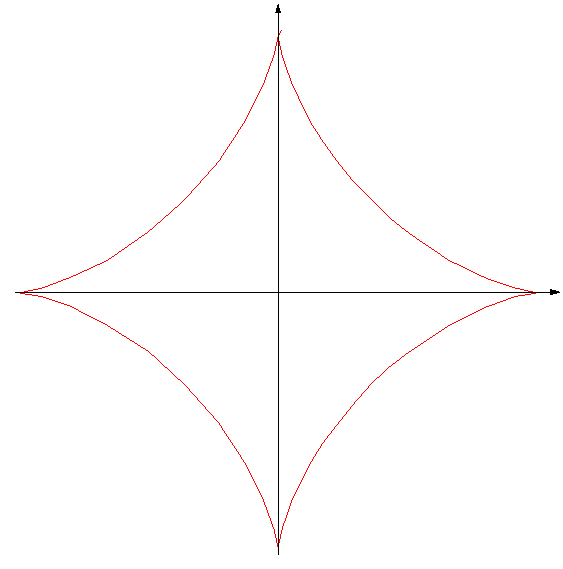
\includegraphics{Castro_2.pdf}
  \caption{Trac{\'e} de l'astro{\"\i}de}
  \label{fig:Castro_2}
\end{figure}
\begin{enumerate}
 \item 
\begin{enumerate}
 \item La courbe est sym{\'e}trique par rapport aux droites passant par l'origine et dirigées par
$\overrightarrow{i}$, $\overrightarrow{j}$, $\overrightarrow{i}+\overrightarrow{j}$.\newline
Les points $M(-t)$, $M(\pi -t)$, $M(\frac{\pi}{2}-t)$ sont respectivement les sym{\'e}triques de $M(t)$ par rapport
aux trois droites.

\item  La courbe est bir{\'e}guli{\`e}re sauf aux points o{\`u} $t$ est congru {\`a} 0 modulo $\frac{\pi }{2}$.\newline
Par raison de sym{\'e}trie, ces points sont des points de rebroussement.\newline
Au point stationnaire $M(0)$, le vecteur tangent est dirigé par la dérivée seconde
\begin{displaymath}
\overrightarrow{M^{\prime \prime }}(0) = -24a\overrightarrow{i} 
\end{displaymath}
Les tangentes aux autres points de rebroussement s'obtiennent par sym{\'e}trie. On peut noter que la tangente en
$M(\frac{\pi }{4})$ est orthogonale {\`a} la premi{\`e}re bissectrice.

\item  En notant $L$ la longueur totale de la courbe et $\overrightarrow{u}_{t}=\cos t\overrightarrow{i}+\sin t\overrightarrow{j}$, on obtient 
\begin{displaymath}
\overrightarrow{M^{\prime }}(t)=-24a\sin t\cos t~\overrightarrow{u}_{-t}=12a\sin 2t\,\overrightarrow{u}_{\pi -t} 
\end{displaymath}
d'o{\`u}
\begin{displaymath}
L = 4\int_{0}^{\frac{\pi }{2}} 
\left\Vert
\overrightarrow{M}'(t)
\right\Vert dt
= 48a\int_{0}^{\frac{\pi }{2}}\sin 2t\,dt = 48a 
\end{displaymath}
\end{enumerate}

\begin{figure}[ht]
  \centering
  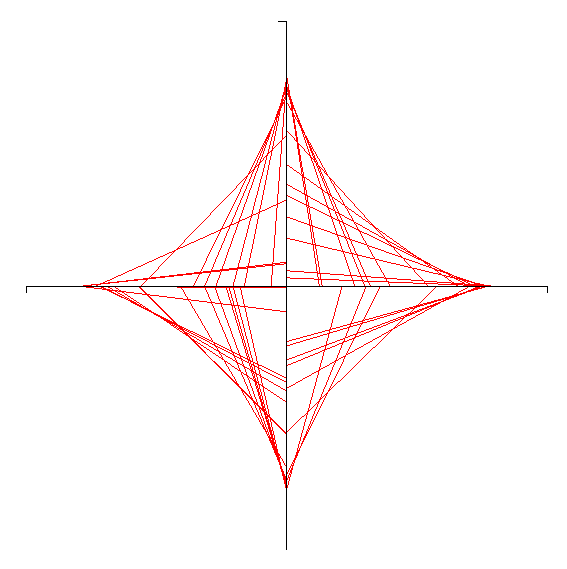
\includegraphics{Castro_1.pdf}
  \caption{Trac{\'e} de 50 segments tangents}
  \label{fig:Castro_1}
\end{figure}

\item
\begin{enumerate}
 \item Lorsque $M(t)$ n'est pas un point singulier, une {\'e}quation de $D(t)$ est
\begin{displaymath}
(x-8a\cos ^{3}t)\sin t+(y-8a\sin ^{3}t)\cos t = 0 \Leftrightarrow
x\sin t+y\cos t = 8a\sin t\cos t
\end{displaymath}


\item  On peut calculer les coordonn{\'e}es de $A(t)$ et $B(t)$. Il vient 
\begin{align*}
 \text{coordonnées de $A(t)$ : } (8a\cos t,0) & &
\text{coordonnées de $B(t)$ : } (0,8a\sin t)
\end{align*}
La longueur du segment $A(t)B(t)$ est donc constante {\'e}gale {\`a} $8a$.\newline
On peut se faire idée des tangentes à l'astroïde en faisant glisser sur les axes les deux extrémités d'un segment de longueur fixe (Fig. \ref{fig:Castro_1}). 

\begin{figure}[ht]
  \centering
  \input{Castro_3.pdf_t}
  \caption{Construction de $D(t_0)$}
  \label{fig:Castro_3}
\end{figure}
\end{enumerate}

\item
\begin{enumerate}
 \item   On cherche les $t$ tels que $D(t)$ contienne le point de coordonn{\'e}es 
\begin{displaymath}
(2a\cos t_{0},2a\sin t_{0}) 
\end{displaymath}
Ils doivent vérifier
\begin{displaymath}
4a\cos t_{0}\sin t+4a\sin t_{0}\cos t = 8a\sin t\cos t \Leftrightarrow
\sin (t+t_{0}) = \sin 2t
\end{displaymath}
La derni{\`e}re {\'e}quation {\'e}quivaut {\`a} 
\begin{align*}
 t=t_{0} &  &\text{ ou }& & t\equiv \frac{\pi -t_{0}}{3} \hspace{1cm}(\frac{\pi }{3})
\end{align*}
La deuxième relation conduit à trois tangentes faisant entre elles un angle de $\frac{\pi }{3}$.\newline
La quatrième tangente est $D(t_{0})$ qui passe par $P_{0}$ et de direction $\,\overrightarrow{u}_{\pi -t}$.

\item  D'après la question précédente, on peut construire la droite $D(t_{0})$ en remarquant qu'elle est sym{\'e}trique de $(OP_{0})$ par rapport {\`a} la droite de direction $\overrightarrow{j}$ qui passe par $P_{0}$. (Fig. \ref{fig:Castro_3})

\begin{figure}[ht]
	\centering
	\input{Castro_4.pdf_t}
	\caption{Construction géométrique de $M_0$}
\label{fig:Castro_4}
\end{figure}

\item  On note avec un indice 0 tous les objets relatifs {\`a} $t_{0}$.\newline
Cherchons $H_{0}=H(t_{0})$ sous la forme 
\begin{displaymath}
 (\lambda \sin t_{0},\lambda \cos t_{0})
\end{displaymath}
pour que $\overrightarrow{OH_0}$ soit orthogonal $D_0$. On remplace dans l'équation de $D_0$ et on obtient 
\begin{displaymath}
\lambda =8a\sin t_{0}\cos t_{0}
\end{displaymath}
puis
\begin{displaymath}
\overrightarrow{OH_{0}}+\overrightarrow{OM_{0}}=8a\,\overrightarrow{u}_{t_{0}}
\end{displaymath}
D{\'e}finissons $K_{0}$ par 
\begin{displaymath}
 \overrightarrow{OH_{0}}+\overrightarrow{OM_{0}}=\overrightarrow{OK_{0}}
\end{displaymath}
Il est sur un cercle deux fois plus grand que $\mathcal C$ et aligné avec $0$ et $P_0$. De plus,
\begin{displaymath}
 \overrightarrow{OM_{0}}=\overrightarrow{H_{0}K_{0}}
\end{displaymath}
donc $(O,M_{0},K_{0},H_{0})$ est un parall{\'e}logramme ce qui entraîne que $M_0$ est symétrique de $H_{0}$ par rapport au centre $P_{0}$ du parallélogramme.\newline
On peut donc construire $M_0$ à partir de $P_0$ (Fig. \ref{fig:Castro_4}) Sur la figure on a fait figurer $K_0$ pour éclairer la démonstration (il est utile à celle-ci mais pas à la construction).
\end{enumerate}
\end{enumerate}
%\clearpage%
\newpage%
\section*{Problème 13}%
\addcontentsline{toc}{section}{Pb 13 : Cosinus d'une variable complexe.}%
\fancyhead[LO,RE]{Corrigés - Pb 13 : Cosinus d'une variable complexe.}%
\begin{enumerate}
  \item Soit $w\in \C$. On note $x = \Re(w)$ et $y = \Im(w)$. On peut écrire
\[
  e^{iw} = e^{i(x+iy)} = e^{ix - y} = \underset{> 0}{\underbrace{e^{-y}}}\, e^{ix}.
\]
On en déduit que $x$ est un argument de $e^{iw}$ et que $\left|e^{iw}\right| = e^{-y}$. 
  \item 
  \begin{enumerate}
    \item Les deux exponentielles sont inverses l'une de l'autre:
\[
  e^{iz} + e^{-iz} - 2 
  = \left( e^{i\frac{z}{2}}\right)^2 + \left( e^{-i\frac{z}{2}}\right)^2 - 2 \left( e^{i\frac{z}{2}}\right) \left( e^{-i\frac{z}{2}}\right)
  = \left( e^{i\frac{z}{2}} - e^{-i\frac{z}{2}}\right)^2
\]

    \item Pour calculer $D$ on commence par faire apparaitre un carré sous le module avec la question précédente avant de développer le carré du module d'une différence ou d'une somme selon la formule du cours.
\begin{displaymath}
 D = \frac{1}{2}\left| e^{i\frac{z}{2}} - e^{-i\frac{z}{2}} \right|^2 \\
= \frac{1}{2}\left( |e^{iz}| + |e^{-iz}| -2\Re(e^{i\frac{z}{2}} \overline{e^{-i\frac{z}{2}}})\right) .
\end{displaymath}

Utilisons les parties réelles et imaginaires.
\begin{displaymath}
 e^{iz} = e^{ib -a} = e^{-a}e^{ib} \Rightarrow |e^{iz}| = e^{-a}.
\end{displaymath}
De même, $|e^{-iz}| = e^{a}$. De plus
\begin{displaymath}
e^{i\frac{z}{2}} \overline{e^{-i\frac{z}{2}}} = e^{i\frac{z}{2}} e^{i\frac{\overline{z}}{2}} 
= e^{i\frac{a}{2}-\frac{b}{2} + i\frac{a}{2} + \frac{b}{2}}
= e^{ia}
\Rightarrow
\Re(e^{i\frac{z}{2}} \overline{e^{-i\frac{z}{2}}}) = \cos a.
\end{displaymath}
On en déduit 
\begin{displaymath}
D= \frac{e^{b} + e^{-b}}{2} - \cos a.
\end{displaymath}
Le calcul est analogue pour la somme et conduit à
\begin{displaymath}
S = \frac{e^{b} + e^{-b}}{2} + \cos a.
\end{displaymath}
En les sommant, on obtient finalement
\begin{displaymath}
 D + S = e^{b} + e^{-b}.
\end{displaymath}

  \end{enumerate}

\end{enumerate}

%
\newpage%
\section*{Problème 14}%
\addcontentsline{toc}{section}{Pb 14 : Famille de courbes paramétrées en polaire.}%
\fancyhead[LO,RE]{Corrigés - Pb 14 : Famille de courbes paramétrées en polaire.}%
\begin{enumerate}
\item  Les supports $\mathcal{C}_{\alpha }$ et $\mathcal{C}_{\alpha +\pi }$ des courbes param{\'e}tr{\'e}es sont {\'e}gaux car 
\begin{displaymath}
r_{\alpha}(t)=r_{\alpha +\pi }(t) 
\end{displaymath}
D'autre part, $\mathcal{C}_{-\alpha }=s_{Oy}(\mathcal{C}_{\alpha })$ car $r_{-\alpha }(t)=-r_{\alpha }(-t)$.

\item  Comme $r(t+3\pi )=-r(t)$ la param{\'e}trisation est $3\pi $ p{\'e}riodique.\newline
Le $\cos $ du d{\'e}nominateur s'annule lorsque 
\begin{displaymath}
 t\equiv \frac{3\pi }{4} \hspace{1cm} (\frac{3\pi }{2})
\end{displaymath}
Un intervalle de longueur $3\pi $ contient donc trois valeurs de $t$ annulant le $\cos $.\newline
Le $\sin $ s'annule lorsque 
\begin{displaymath}
 t\equiv 3\alpha \hspace{1cm} (3\pi)
\end{displaymath}
Un intervalle de longueur $3\pi $ contient donc une seule valeur de $t$ annulant le $\sin $.\newline
Comme $\alpha \in \left[ 0,\frac{\pi }{2}\right] $ choisissons $\left[ 0,3\pi\right] $ comme intervalle pour d'étude $t$. Il y a alors trois branches infinies pour les valeurs suivantes du paramètre
\begin{align*}
 \frac{3\pi }{4} & &
 \frac{9\pi }{4}=\frac{\pi}{4}+2\pi & &
3\alpha 
\end{align*}
\begin{itemize}
\item  En $\frac{3\pi }{4}$. Comme
\begin{displaymath}
 \cos \frac{2t}{3} = \sin (\frac{\pi }{2}-\frac{2t}{3})
 = \sin (\frac{2}{3}(\frac{3\pi }{4}-t))
 \sim \frac{2}{3}(\frac{3\pi }{4}-t)
\end{displaymath}
On d{\'e}duit que $r(t)\sin (t-\frac{3\pi }{4})$ diverge vers $+\infty $ ou $-\infty $ d'un c{\^o}t{\'e} ou de l'autre de $\frac{3\pi }{4}$.\newline
Il n'y a donc pas d'asymptote mais seulement une branche parabolique de direction asymptotique
\begin{displaymath}
 \overrightarrow{u}_{\frac{3\pi }{4}}
\end{displaymath}

\item  En $\frac{9\pi }{4}=\frac{\pi }{4}+2\pi $. La situation est analogue.\newline
Il n'y apas d'asymptote mais une branche parabolique de direction asymptotique
\begin{displaymath}
 \overrightarrow{u}_{\frac{\pi }{4}}
\end{displaymath}

\item  En $3\alpha $. On a en revanche 
\begin{displaymath}
 \sin (t-3\alpha )=\sin (3(\frac{t}{3} -\alpha ))\sim 3(\frac{t}{3}-\alpha ) 
\Rightarrow \rho (t)\sin (\frac{t}{3}-\alpha )\sim \frac{3a\cos \alpha }{\cos ^{2}2\alpha }
\end{displaymath}
Il existe donc une asymptote.\newline
Pour étudier la position de la courbe par rapport {\`a} l'asymptote, posons 
\begin{displaymath}
u=\frac{t}{3}-\alpha  
\end{displaymath}
et formons un d{\'e}veloppement limit{\'e} de $r(t)\sin (t-3\alpha )$ suivant $u$. On obtient
\begin{displaymath}
 \frac{a\cos \alpha \sin 3u}{\cos ^{2}(2\alpha +2u)\sin u} 
= 3a\frac{\cos \alpha }{\cos ^{2}2\alpha } + \left( 12a\frac{\cos \alpha }{\cos ^{3}2\alpha }\sin 2\alpha \right) u+u\epsilon (u)
\end{displaymath}
On en d{\'e}duit que la courbe est, suivant le signe de $u$, d'un c{\^o}t{\'e} ou de l'autre de l'asymptote. On remarque aussi que le coefficient de $u$ change de signe lorsque $\alpha $ traverse la valeur $\frac{\pi }{4}$ pour laquelle il n'y a pas d'asymptote.
\end{itemize}

\begin{figure}[ht]
  \centering
  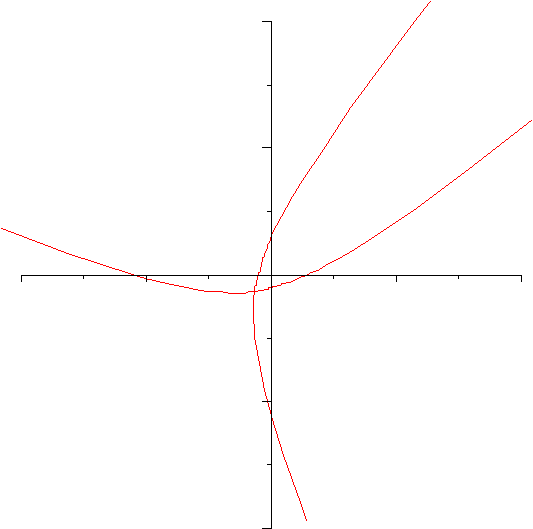
\includegraphics[width=9cm]{Ccurv1_1.pdf}
  \caption{Tracé de $\mathcal C_\frac{\pi}{4}$pour $a=1$}
  \label{fig:Ccurv1_1}
\end{figure}
\item  Le trac{\'e} de la courbe (Fig. \ref{fig:Ccurv1_1}) se fait {\`a} la machine en remarquant que $r(t)$ est n{\'e}gatif dans $\left[0,\frac{3\pi }{4}\right] $ et positif dans $\left[ \frac{3\pi }{4},3\pi \right] $. Le changement
de signe se fait "{\`a} l'infini". La courbe ne passe pas par l'origine.\newline
Comme $\alpha =\frac{\pi }{4}$, $3\alpha =\frac{3\pi }{4}$, il n'y a donc pas d'asymptote mais seulement deux branches paraboliques.

\item Un point est birégulier lorsque la vitesse et l'accélération en ce point forment une famille libre.\newline Notons $f$ la paramétrisation, exprimons la vitesse et l'accélération puis le déterminant :
\begin{align*}  
 f(t) =& 0 + r(t) \overrightarrow e_t \\
 \overrightarrow f'(t) =& r'(t) \overrightarrow e_t +r(t) \overrightarrow e_{t+\frac{\pi}{2}} \\
\overrightarrow f''(t) =& (r''(t) -r(t))\overrightarrow e_t + 2r'(t) \overrightarrow e_{t+\frac{\pi}{2}} \\
\det(\overrightarrow f'(t),\overrightarrow f''(t)) =&
\begin{vmatrix}
 r'(t) & r''(t) -r(t)  \\
 r(t) & 2r'(t)
\end{vmatrix}
\end{align*}
La condition assurant la non bir{\'e}gularit{\'e} s'{\'e}crit donc
\begin{displaymath}
 2r'^2 -rr''+r^2=0
\end{displaymath}
En posant $\lambda =\frac{1}{r}$, cette condition devient 
\begin{displaymath}
\lambda +\lambda ''=0 
\end{displaymath}
Pour l'exprimer simplement dans le cas particulier qui nous est demandé, on commence par lin{\'e}ariser $\lambda $. Il vient
\begin{displaymath}
\lambda  = \frac{1}{2}\sin (\frac{t}{3}-\alpha ) 
+ \frac{1}{4}\sin (\frac{5t}{3}-\alpha )
-\frac{1}{4}\sin (t+\alpha )
\end{displaymath}
puis
\begin{multline*}
\lambda +\lambda'' = \frac{1}{2}(1-\frac{1}{9})\sin (\frac{t}{3}-\alpha )+\frac{1}{4}(1-\frac{25}{9})\sin (\frac{5t}{3}-\alpha ) \\
 = \frac{4}{9}\sin (\frac{t}{3}-\alpha )-\frac{4}{9}\sin (\frac{5t}{3}-\alpha ) 
 = -\frac{8}{9}\cos (t-\alpha )\sin (\frac{2t}{3})
\end{multline*}
Cette expression est nulle lorsque 
\begin{displaymath}
t-\alpha \equiv \frac{\pi }{2} \hspace{1cm} (\pi)  
\end{displaymath}
Lorsque $\alpha $ varie le point tel que $t-\alpha \equiv \frac{\pi }{2}$ modulo $\pi$ d{\'e}crit la courbe param{\'e}tr{\'e}e
\[
r(t)=-\frac{a\sin t}{\cos ^{3}\frac{2t}{3}}
\]
\end{enumerate}
%
\newpage%
\section*{Problème 15}%
\addcontentsline{toc}{section}{Pb 15 : Développements limités de puissance de puissance.}%
\fancyhead[LO,RE]{Corrigés - Pb 15 : Développements limités de puissance de puissance.}%
\begin{enumerate}
\item Par définition 
\[u(x)=e^{x\ln |x|}, v(x)=e^{x^{2}\ln |x|}, w(x)=e^{u(x)\ln |x|}\]
Les limites usuelles en 0, en particulier $x^{k}\ln |x|\rightarrow 0$, entrainent
\[u_{0}=1,\quad v_{0}=1,\quad w_{0}=0\] 
\item\begin{enumerate}
\item En $+\infty$, $x\ln |x|\rightarrow +\infty$ donc les trois fonctions divergent vers $+\infty$.
\item \'{E}tude des dérivabilités en 0. \newline
Comme $x\ln |x|\rightarrow 0$, $\frac{u(x)-1}{x}\sim \ln |x|\rightarrow +\infty$  donc $u$ n'est pas dérivable en 0.\newline
De même $\frac{v(x)-1}{x}\sim x\ln |x|\rightarrow 0$ donc $v$ est dérivable en 0.\newline
Enfin, pour $x>0$,
\[
\frac{w(x)}{x}=e^{(u(x)-1)\ln |x|} \text{ avec } (u(x)-1)\ln x\sim x \ln^{2} x
\]
donc $\frac{w(x)}{x}$ converge vers 1 à droite de 0. Mais pour $x<0$
\[
\frac{w(x)}{x}=- e^{(u(x)-1)\ln |x|}\rightarrow -1 \text{ donc $w$ n'est pas dérivable en 0.}
\]

\item Les développements limités s'obtiennent par composition.
\newline En 1
\begin{align*}
u(x) &= 1 + (x-1) + (x-1)^{2} + \frac{1}{2}(x-1)^{3} + o((x-1)^{3})\\
v(x) &= 1 + (x-1) + 2(x-1)^{2} + 2(x-1)^{3} + o((x-1)^{3})\\
w(x) &= 1 + (x-1) + (x-1)^{2} + \frac{3}{2}(x-1)^{3} + o((x-1)^{3})
\end{align*}
En -1
\begin{align*}
u(x) &= 1 + (x+1) - \frac{1}{2}(x+1)^{3} + o((x+1)^{3})\\
v(x) &= 1 -(x+1) + 2(x+1)^{2} - 2(x+1)^{3} + o((x+1)^{3})\\
w(x) &= 1 -(x+1) - (x+1)^{2} + \frac{1}{2}(x+1)^{3} + o((x+1)^{3}).
\end{align*}
\end{enumerate}

\end{enumerate}


%
\newpage%
\section*{Problème 16}%
\addcontentsline{toc}{section}{Pb 16 : Fonctions usuelles et polynômes de Chebychev.}%
\fancyhead[LO,RE]{Corrigés - Pb 16 : Fonctions usuelles et polynômes de Chebychev.}%
\subsection*{Exercice 1}
\begin{enumerate}
  \item Expressions de $\tan \frac{\pi}{8}$ et $\tan \frac{3\pi}{8}$ avec des racines carrées.
\begin{enumerate}
  \item Lorsque $x \not \equiv \frac{\pi}{2} \mod \pi$ et $x \not \equiv \pi \mod 2\pi$, on peut écrire
\[
  \tan x = \frac{2 \tan \frac{x}{2}}{1 - \tan^2 \frac{x}{2}}.
\]
 \item Introduisons $\epsilon = \pm 1$ pour rendre compte synthétiquement de $\tan \frac{\pi}{4} = 1$ et $\tan \frac{3\pi}{4} = -1$. En utilisant la formule précédente, considèrons l'équation d'inconnue $t$ réelle
\[
  \epsilon = \frac{2t}{1-t^2} \Leftrightarrow 1 = \epsilon \, \frac{2t}{1-t^2} \Leftrightarrow t^2 + 2\epsilon t - 1 = 0\;(E_\epsilon).
\]
Alors $\tan \frac{\pi}{8}$ est la solution positive de l'équation $(E_\epsilon)$ avec $\epsilon = 1$ et $\tan \frac{3\pi}{8}$ est la solution positive de l'équation avec $\epsilon = -1$.\newline
Les solutions de l' équation $(E_\epsilon)$ sont $-\epsilon \pm \sqrt{2}$. On en déduit
\[
  \tan \frac{\pi}{8} = -1 + \sqrt{2}, \hspace{0.5cm} \tan \frac{3\pi}{8} = 1 + \sqrt{2}.
\]
Les autres solutions sont
\[
  1 - \sqrt{2} = \tan \left( -\frac{\pi}{8}\right),\hspace{0.5cm}
  -1 - \sqrt{2} = \tan \left( -\frac{3\pi}{8}\right).
\]
\end{enumerate}
Comme les arguments sont entre $-\frac{\pi}{2}$ et $\frac{\pi}{2}$, on obtient le tableau 
\begin{center}
\renewcommand{\arraystretch}{1.5}
\begin{tabular}{|l|c|c|c|c|} \hline
solutions & $-1-\sqrt{2}$     & $1-\sqrt{2}$     & $-1+\sqrt{2}$   & $1 + \sqrt{2}$    \\ \hline
$\arctan$ & $-\frac{3\pi}{8}$ & $-\frac{\pi}{8}$ & $\frac{\pi}{8}$ & $\frac{3\pi}{8}$ \\ \hline
\end{tabular}
\end{center}

\item
\begin{enumerate}
  \item On suppose que $t$ n'est pas congru {\`a} $\frac{\pi }{8}$ modulo $\frac{\pi }{4}$ ni {\`a} $\frac{\pi }{2}$ modulo $\pi $ donc $\tan 4t$ et $\tan t$
sont bien d{\'e}finis. Avec la formule du binôme:
\begin{multline*}
\cos 4t = \Re (\cos t+i\sin t)^{4} = \cos ^{4}t-6\cos^{2}t\sin^{2}t+\sin ^{4}t \\
 = \cos ^{4}t\,\left(1-6\tan ^{2}t+\tan^{4}t\right),
\end{multline*}
\begin{multline*}
\sin 4t = \Im (\cos t+i\sin t)^{4} = 4\cos ^{3}t\sin t-4\cos t\sin^{3}t\\
 = \cos ^{4}t\,\left(4\tan t-4\tan ^{3}t\right).
\end{multline*}
On en d{\'e}duit
\[
\tan 4t=\frac{4\tan t-4\tan ^{3}t}{1-6\tan ^{2}t+\tan ^{4}t}.
\]

  \item On sait que $\cos 4t = 0 \Leftrightarrow t \equiv \frac{\pi}{8} \mod \frac{\pi}{4}$. Pour de tels $t$, $\cos t \neq 0$ et $\tan t$ est racine de $1-6x^2 + x^4=0$. On en déduit que 
\[
  -1-\sqrt{2} = \tan(-\frac{3\pi}{8}) < 1 - \sqrt{2} = \tan(-\frac{\pi}{8}) < - 1 + \sqrt{2} = \tan\frac{\pi}{8} <  1 + \sqrt{2} = \tan\frac{3\pi}{8} 
\]
sont quatre racines distinctes de cette équation. Ce sont les seules car l'équation est de degré 4. 
  
  \item Pour $x\notin \left\{ -1 - \sqrt{2}, 1 - \sqrt{2}, -1 + \sqrt{2}, 1+\sqrt{2}\right\}$, la fraction est définie. De plus, en notant $t=\arctan x$ ce qui entraine $x=\tan t$, la question a. montre que
\[
\frac{4x^{2}-4x^{3}}{1-6x^{2}+x^{4}} = \tan 4t.
\]
On ne peut pas en déduire que 
\[
\arctan \left(\frac{4x^{2}-4x^{3}}{1-6x^{2}+x^{4}}\right) = 4t = 4\arctan x
\]
car $4t$ n'est pas toujours dans $\left] -\frac{\pi}{2}, \frac{\pi}{2} \right[$ suivant les valeur de $t$. Il faut considérer divers cas et ajouter le bon multiple de $\pi$.

\begin{description}
  \item[.] Si $x<-1 - \sqrt{2}$ alors $t\in \left] -\frac{\pi}{2},-\frac{3\pi }{8}\right[$, 
  $4t\in \left] -2\pi ,-\frac{3\pi}{2}\right[$, $4t+2\pi \in \left] -\frac{\pi }{2},\frac{\pi}{2}\right[$ .
  \item[.] Si $-1 - \sqrt{2}<x< 1 - \sqrt{2}$ alors $t\in \left] -\frac{3\pi }{8},-\frac{\pi }{8}\right[$,
  $4t\in \left] -\frac{3\pi }{2},-\frac{\pi }{2}\right[ $, $4t+\pi \in \left] -\frac{\pi }{2}, \frac{\pi }{2}\right[$.
  \item[.]  Si $1-\sqrt{2}<x<-1+\sqrt{2}$ alors $t\in \left]-\frac{\pi }{8},\frac{\pi }{8}\right[$,
  $4t\in \left] - \frac{\pi}{2},-\frac{\pi }{2}\right[$.
  \item[.] Si $-1 + \sqrt{2 } < x <1+\sqrt{2}$ alors $t\in \left] \frac{\pi }{8},\frac{3\pi }{8}\right[$,
  $4t\in \left]\frac{\pi }{2},\frac{3\pi }{2}\right[ $, $4t-\pi \in \left] -\frac{\pi }{2},\frac{\pi }{2}\right[$.
  \item[.] Si $1+\sqrt{2} < x$ alors $t\in \left] \frac{3\pi }{8},\frac{\pi }{2}\right[$,
  $4t\in \left] \frac{3\pi }{2},2\pi \right[ $, $4t-2\pi \in \left] -\frac{\pi }{2},\frac{\pi }{2}\right[$.
\end{description}
Finalement :
\[
\arctan \frac{4x^{2}-4x^{3}}{1-6x^{2}+x^{4}} = 4\arctan x \;
\left\{
\begin{aligned}
&+2\pi  &\text{si} & & &x < -1 - \sqrt{2}  \\
&+\pi   &\text{si} & &-1 - \sqrt{2} < &x < 1 - \sqrt{2}  \\
&+0     &\text{si} & &1 - \sqrt{2} < &x < -1 + \sqrt{2}  \\
&-\pi   &\text{si} & &-1 + \sqrt{2} < &x < 1 + \sqrt{2} \\
&-2\pi  &\text{si} & &1 + \sqrt{2} < &x 
\end{aligned}
\right.
\]
\end{enumerate}
\end{enumerate}

\subsection*{Exercice 2}
\begin{enumerate}
\item  A l'aide de la formule de r{\'e}currence, on obtient
imm{\'e}diatement
\begin{eqnarray*}
P_{2}(t) &=&2t^{2}-1 \\
P_{3}(t) &=&2t(2t^{2}-1)-t=4t^{3}-3t \\
P_{4}(t) &=&2t(4t^{3}-3t)-(2t^{2}-1)=8t^{4}-8t^{2}+1 \\
Q_{2}(t) &=&2t \\
Q_{3}(t) &=&2t(2t)-1=4t^{2}-1 \\
Q_{4}(t) &=&2t(4t^{2}-1)-2t=8t^{3}-4t
\end{eqnarray*}

\item  On remarque que les formules sont vraies pour $n=0$ et $1$. En effet:
\[
\forall x \in \R, \; 
\left\lbrace
\begin{aligned}
  &P_0(\cos x) = 1 = \cos(0x), &P_1(\cos x) = \cos x = \cos(1x) \\
  &\sin x \,Q_0(\cos x) = 0 = \sin(0x), &\sin x \, Q_1(\sin x) = \sin x = \sin(1x) 
\end{aligned}
\right. .
\]
Pour tout $n\in \N$, considérons la propriété $\mathcal{C}_n$:
\[
  \forall x \in \R, \hspace{0.5cm}
  \left\lbrace
    \begin{aligned}
      &P_{n}(\cos x) = \cos (nx),& &\sin x\,Q_{n}(\cos x)=\sin (nx) \\
      &P_{n+1}(\cos x) = \cos ((n+1)x),& &\sin x\,Q_{n+1}(\cos x) = \sin ((n+1)x)
    \end{aligned}
  \right.
\]
Comme on a vu que $\mathcal{C}_0$ est vraie, il s'agit de montrer que $\left( \forall n \in \N, \; \mathcal{C}_n \Rightarrow \mathcal{C}_{n+1}\right)$. En fait, par définition de la proposition, il suffit de démontrer
\[
  \mathcal{C}_n \Rightarrow
  \left\lbrace
  \begin{aligned}
    P_{n+2}(\cos x)         &= \cos ((n+2)x) \\
    \sin x\,Q_{n+2}(\cos x) &= \sin ((n+2)x)
  \end{aligned}
  \right. .
\]
Utilisons les formules de transformation de somme en produit :
\[
\begin{aligned}
\cos ((n+2)x)+\cos nx &= 2\cos x\cos ((n+1)x) \\
\sin ((n+2)x)+\sin nx &= 2\cos x\sin ((n+1)x)
\end{aligned}
\]
d'o{\`u}
\[
\cos ((n+2)x)=2\cos xP_{n+1}(\cos x)-P_{n}(\cos x)=P_{n+2}(\cos x)
\]
d'apr{\`e}s la formule d{\'e}finissant $P_{n+2}$. De m{\^e}me,
\[
\sin ((n+2)x)=2\cos x\sin x\,Q_{n+1}(\cos x)-\sin x\,Q_{n}(\cos
x)=\sin xQ_{n+2}(x)
\]
d'apr{\`e}s la formule d{\'e}finissant $Q_{n+2}$.

\item  D{\'e}rivons l'égalité fonctionelle $P_n(\cos x) = cantberns (nx)$ de la pr{\'e}c{\'e}dente. Il vient
\[
-\sin xP_{n}^{\prime }(\cos x)=-n\sin nx.
\]
Ce qui s'{\'e}crit encore
\[
-\sin xP_{n}^{\prime }(\cos x)=-n\sin x\,Q_{n}(\cos x).
\]
Lorsque $x\in \left] 0,\pi \right[ $, $\sin x$ est non nul et on obtient $ P_{n}^{\prime }(\cos x)=n\,Q_{n}(\cos x)$. Pour tout r{\'e}el $t$ dans $\left] -1,1\right[ $, il existe un $x\in \left] 0,\pi \right[ $ tel que $t=\cos x$, on en d{\'e}duit la formule demand{\'e}e.
\end{enumerate}
%
\newpage%
\section*{Problème 17}%
\addcontentsline{toc}{section}{Pb 17 : Exercices: coefficients du binôme, inéquation à paramètre.}%
\fancyhead[LO,RE]{Corrigés - Pb 17 : Exercices: coefficients du binôme, inéquation à paramètre.}%
\begin{enumerate}
  \item Pour $k\geq 1$, on peut {\'e}crire
\begin{displaymath}
 (k+1)\binom{n}{k} = k \binom{n}{k} + \binom{n}{k} = n \binom{n-1}{k-1} + \binom{n}{k} 
\end{displaymath}
d'o{\`u} , en notant $S$ la somme cherch{\'e}e :
\begin{displaymath}
 S=n\sum_{k=1}^n\binom{n-1}{k-1}+\sum_{k=0}^n\binom{n}{k}= n2^{n-1}+2^n = (n+2)2^{n-1}
\end{displaymath}
Autre solution. Consid{\'e}rons la fonction $f$ définie par $f(x)=x(1+x)^n$. Alors $S=f'(1)$ or $f'(x)=(1+x)^n+nx(1+x)^{n-1}$ d'où $S=2^n+n2^{n-1}$.

\item Factorisons la différence. 
\begin{multline*}
  (m+2)x+1 - \frac{1+x+x^2}{1-x} = \frac{(m+2)x+1-(m+2)x^2 -x-1-x-x^2}{1-x}\\
  = \frac{mx-(m+3)x^2}{1-x} = \frac{\left((m+3)x-m \right)x }{x-1}
\end{multline*}
L'in{\'e}quation propos{\'e}e est {\'e}quivalente (pour $m\neq -3$) {\`a}
\begin{displaymath}
 \frac{m+3}{x-1}x(x-h(m))<0 \text{ avec } h(m)=\frac{m}{m+3}= 1-\frac{3}{m+3}
\end{displaymath}
\begin{figure}[h!t]
 \centering
 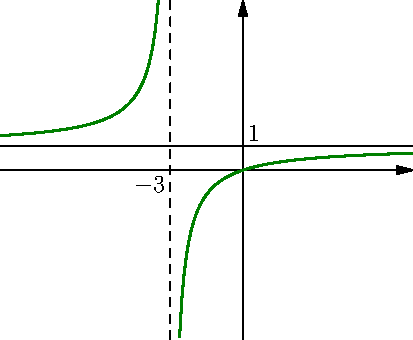
\includegraphics{./Celem5_1.pdf}
 \caption{Graphe de $h$}
 \label{fig:Celem5_1}
\end{figure}
Le signe de cette expression est facile à évaluer pour $x$ plus grand que $0, 1, h(m)$ et elle change de signe en chacune de ces valeurs. On doit donc classer 0, 1, $h(m)$ suivant $m$ en étudiant le graphe de $h$ qui est une hyperbole. (fig \ref{fig:Celem5_1}). On obtient:
\begin{itemize}
  \item Si $m < -3$,
\begin{displaymath}
0 < 1 < h(m)\hspace{0.5cm}\Rightarrow \hspace{0.5cm} \mathcal{S}_m = \,]0,1[\, \cup \, ]\frac{m}{m+3},+\infty[  
\end{displaymath}

  \item Si $m=-3$, l'inéquation devient
\begin{displaymath}
  \frac{3x}{x-1}<0  \hspace{0.5cm}\Rightarrow \hspace{0.5cm} \mathcal{S}_m = \,]0, 1[
\end{displaymath}

  \item Si $-3 < m \leq 0$
\begin{displaymath}
h(m) < 0 < 1 \hspace{0.5cm}\Rightarrow \hspace{0.5cm} \mathcal{S}_m =\, ]-\infty, \frac{m}{m+3}[\, \cup \, ]0,1[   
\end{displaymath}

  \item Si $m>0$
\begin{displaymath}
0 < h(m) < 1 \hspace{0.5cm}\Rightarrow \hspace{0.5cm} \mathcal{S}_m =\, ]-\infty,0[\, \cup \, ]\frac{m}{m+3},1 [   
\end{displaymath}
\end{itemize}

\item Les $k!$ et $(k+1)!$ se simplifient respectivement dans les deux quotients en permettant une mise en facteur
  \begin{multline*}
  \frac{\binom{n}{k}}{\binom{2n}{k}}-\frac{\binom{n}{k+1}}{\binom{2n}{k+1}}
  = \frac{n(n-1)\cdots (n-k+1)}{(2n)(2n-1)\cdots  (2n-k+1)} - \frac{n(n-1)\cdots (n-k)}{(2n)(2n-1)\cdots  (2n-k)}\\
  = \frac{n(n-1)\cdots (n-k+1)}{(2n)(2n-1)\cdots  (2n-k+1)}(1-\frac{n-k}{2n-k})\\
  = \frac{n (n-1)\cdots (n-k+1)}{(2n)(2n-1)\cdots (2n-k+1)}\frac{n}{2n-k}
  = \frac{1}{2}\,\frac{n(n-1)(n-2)\cdots(n-k+1)}{(2n-1)(2n-2)\cdots(2n-k)}
  \end{multline*}
  Ce quotient contient $k$ facteurs en haut (compteur entre $0$ et $k-1$) et en bas (compteur entre $1$ et $k$). On retrouve un quotient de coefficients du bin{\^o}me en introduisant des $k!$ en haut et en bas. On en d{\'e}duit la formule valable pour $k$ entre 0 et $n-1$
  \begin{displaymath}
  \frac{\binom{n}{k}}{\binom{2n}{k}}-\frac{\binom{n}{k+1}}{\binom{2n}{k+1}}
  =\frac{1}{2}\frac{\binom{n}{k}}{\binom{2n-1}{k}}
  \end{displaymath}
  Dans le calcul de la somme $S$, il faut traiter {\`a} part le dernier terme.
  \begin{displaymath}
  S =
  2\left( \frac{\binom{n}{0}}{\binom{2n}{k}}-\frac{\binom{n}{n}}{\binom{2n}{n}}\right) 
+\frac{\binom{n}{n}}{\binom{2n-1}{n}}
  = 2\left( 1-\frac{1}{\binom{2n}{n}}\right) +\frac{1}{\binom{2n-1}{n}}
  \end{displaymath}
Or  
\begin{displaymath}
 \binom{2n-1}{n-1}+\binom{2n-1}{n}=\binom{2n}{n}
\text{ avec }
\binom{2n-1}{n-1}= \binom{2n-1}{n}
\end{displaymath}
donc
\begin{displaymath}
 \binom{2n}{n} = 2 \binom{2n-1}{n}\text{ et } S=2 
\end{displaymath}

\end{enumerate}
%
\newpage%
\section*{Problème 18}%
\addcontentsline{toc}{section}{Pb 18 : Fractions rationnelles : décomposition en éléments simples.}%
\fancyhead[LO,RE]{Corrigés - Pb 18 : Fractions rationnelles : décomposition en éléments simples.}%
\begin{enumerate}
 \item Les pôles de $F$ sont les racines $n$-ièmes de $1$. Comme la fraction est de degré strictement négatif, il n'y a pas de partie entière. La fraction est la somme de ses parties polaires.
 \item Le développement limité de $x^k$ en $1$ est
\begin{displaymath}
 x^k = 1 +k(x-1) + o(x-1)
\end{displaymath}
En sommant les développements précédents, la somme des entiers consécutifs apparait et il vient:
\begin{displaymath}
 1+x+\cdots +x^{n-1} = n +\frac{n(n-1)}{2}(x-1)+o(x-1)
\end{displaymath}
On factorise par $n$ pour se ramener à un développement usuel
\begin{multline*}
 \frac{1}{(1+x+\cdots +x^{n-1})^2}=\frac{1}{n^2}\left(1+\frac{n-1}{2}(x-1)+o(x-1) \right)^{-2}\\
=\frac{1}{n^2} -\frac{n-1}{n^2}(x-1)+o(x-1) 
\end{multline*}

 \item Soit $u\in\U$. Si on substitue $uX$ à $X$ dans $F$, la fraction est conservée. La partie polaire relative au pôle $u$ devient
\begin{displaymath}
 \frac{\alpha(u)}{(uX-u)^2}+\frac{\beta(u)}{uX-u}=
\frac{\alpha(u)}{u^2(X-1)^2}+\frac{\beta(u)}{u(X-1)}
\end{displaymath}
qui est la partie polaire relative à $1$. On en déduit
\begin{displaymath}
 \alpha(u) = u^2\alpha(1),\hspace{1cm} \beta(u)=u\beta(1)
\end{displaymath}

 \item
\begin{enumerate}
 \item Par définition d'une partie polaire,
\begin{displaymath}
 F = \frac{\alpha(1)}{(X-1)^2} + \frac{\beta(1)}{X-1} +R
\end{displaymath}
où $R$ est une fraction qui n'admet pas de pôle en $1$. Comme
\begin{displaymath}
 X^n-1 = (X-1)(1+X+\cdots+X^{n-1})
\end{displaymath}
En multipliant $F$ par $(X-1)^2$, on obtient
\begin{displaymath}
 \frac{1}{(1+X+\cdots+X^{n-1})^2} = \alpha(1)+\beta(1)(X-1)+(X-1)^2R
\end{displaymath}
Comme $1$ n'est pas un pôle de $R$, la fonction attachée à $R$ admet une limite finie en $1$ dont la fonction attachée à$(X-1)^2R$ est négligeable en $1$ devant $x-1$. L'écriture proposée est donc bien un développement limité en $1$.
 \item En identifiant les développements limités obtenus en 2. et 4.a., on obtient
\begin{displaymath}
 \alpha(1)=\frac{1}{n^2},\hspace{1cm}\beta(1)=-\frac{n-1}{n^2}
\end{displaymath}
puis la décomposition en éléments simples
\begin{displaymath}
 F= \frac{1}{n^2}\sum_{u\in\U}\frac{u^2}{(X-u)^2} - \frac{n-1}{n^2}\sum_{u\in\U}\frac{u}{X-u}
\end{displaymath}
\end{enumerate}

 \item
\begin{enumerate}
 \item Si $1\leq k \leq n-1$ et $k'=n-k$, alors $1\leq k' \leq n-1$ et $\overline{w^k}=w^{k'}$.
 \item On regroupe les racines conjuguées. Dans le cas pair deux racines sont réelles ($1$ et $-1$) dans le cas impair $1$ est la seule racine.
\begin{align*}
 n=2p& &X^n-1 &= (X-1)(X+1)\prod_{k=1}^{p-1}\left(X^2-2\cos\frac{2k\pi}{n}X +1 \right) \\ 
 n=2p+1& &X^n-1 &= (X-1)\prod_{k=1}^{p}\left(X^2-2\cos\frac{2k\pi}{n}X +1 \right) 
\end{align*}

 \item Pour un pôle $u=e^{i\theta}$ non réel, 
\begin{displaymath}
 \frac{u^2}{(X-u)^2}= \frac{u^2(X^2-2\overline{u}X+\overline{u}^2)}{(X^2-2\cos\theta X +1)^2}
=\frac{u^2X^2-2uX+1}{(X^2-2\cos\theta X +1)^2}
\end{displaymath}
Les éléments simples relatifs à deux pôles conjugués sont eux mêmes conjugués. Les regrouper revient à prendre deux fois la partie réelle. Soit:
\begin{multline*}
 2\frac{\cos2\theta X^2 -2\cos\theta X +1}{(X^2-2\cos\theta X +1)^2}\\
= \frac{2\cos 2\theta }{X^2-2\cos\theta X +1} +4\sin^2\theta\frac{-2\cos \theta X +1}{(X^2-2\cos\theta X +1)^2}
\end{multline*}
Pour le résidu,
\begin{displaymath}
 \frac{u}{X-u}=\frac{u(X-\overline{u})}{X^2-2\cos\theta X +1}=\frac{uX-1}{X^2-2\cos\theta X +1}
\end{displaymath}
Le double de la partie réelle est 
\begin{displaymath}
 2\frac{\cos \theta X-1}{X^2-2\cos\theta X +1}
\end{displaymath}
On en déduit la décomposition dans $\R(X)$. On pose $\theta_k= \frac{2k\pi}{n}$.\newline
Dans le cas impair $n=2p+1$:
\begin{multline*}
 F=\frac{1}{n^2}\frac{1}{(X-1)^2}-\frac{n-1}{n^2}\frac{1}{X-1}\\
+\frac{4}{n^2}\sum_{k=1}^p\sin^2\theta_k\frac{-2\cos \theta_k X +1}{(X^2-2\cos\theta_k X +1)^2}\\
+\frac{2}{n^2}\sum_{k=1}^p\frac{(n-1)\cos \theta_k X +n-1+\cos 2\theta_k}{X^2-2\cos\theta_k X +1}
\end{multline*}
Dans le cas pair $n=2p$:
\begin{multline*}
 F=\frac{1}{n^2}\frac{1}{(X-1)^2}-\frac{n-1}{n^2}\frac{1}{X-1}
+\frac{1}{n^2}\frac{1}{(X+1)^2}+\frac{n-1}{n^2}\frac{1}{X+1}\\
+\frac{4}{n^2}\sum_{k=1}^{p-1}\sin^2\theta_k\frac{-2\cos \theta_k X +1}{(X^2-2\cos\theta_k X +1)^2}\\
+\frac{2}{n^2}\sum_{k=1}^{p-1}\frac{(n-1)\cos \theta_k X +n-1+\cos 2\theta_k}{X^2-2\cos\theta_k X +1}
\end{multline*}
\end{enumerate}

\end{enumerate}
%
\newpage%
\section*{Problème 19}%
\addcontentsline{toc}{section}{Pb 19 : Polynômes symétriques élémentaires.}%
\fancyhead[LO,RE]{Corrigés - Pb 19 : Polynômes symétriques élémentaires.}%
Introduisons les polynômes symétriques élémentaires
\begin{align*}
 \sigma_1 = x_1+x_2+x_3 & & \sigma_2 = x_1x_2+x_1x_3+x_2x_3 & & \sigma_3=x_1x_2x_3
\end{align*}
et utilisons les pour exprimer chacune des trois relations.\newline
La première relation donne immédiatement $\sigma_1^2 -2\sigma_2 = 1$. \newline
On obtient la deuxième relation en réduisant au même dénominateur $x_1x_2x_3$:
\begin{displaymath}
 \frac{\sigma_1}{\sigma_3}=\frac{3}{2}
\end{displaymath}
Pour la troisième, on commence par regrouper par trois les termes qui ont le même dénominateur. Cela fait apparaitre le $\sigma_1$ au numérateur que l'on peut mettre en facteur:
\begin{displaymath}
 (x_1+x_2+x_3)\left( \frac{1}{x_1}+\frac{1}{x_2}+\frac{1}{x_3}\right) =6
\end{displaymath}
On réduit au même dénominateur $x_1x_2x_3$ ce qui donne directement: $\frac{\sigma_1\sigma_2}{\sigma_3}=6$.\newline
\`A partir des deux dernières relations, on obtient $\sigma_2=4$.\newline
En remplaçant dans la première, on obtient
\begin{displaymath}
 \sigma_1^2 = 9
\end{displaymath}
Le dernier s'obtient à partir de $\sigma_1$: $\sigma_3 = \frac{2}{3}\sigma_1$. 
On a donc deux possibilités:
\begin{align*}
 \sigma_1&=3 & \sigma_3&=2 & \sigma_2&= 4 \\
 \sigma_1&=-3 & \sigma_3&=-2 & \sigma_2&= 4 
\end{align*}
Les nombres $x_1$, $x_2$, $x_3$ sont donc (à permutation près) les racines des polynômes
\begin{displaymath}
 X^3-3X^2+4X-2, \hspace{1cm} X^3+3X^2+4X+2
\end{displaymath}
après factorisation à l'aide de la racine évidente $1$ ou $-1$ avec une division par $X-1$ ou $X+1$, on obtient les triplets $(1, 1 + i,1 - i)$ et $(-1,-1 + i,-1 - i)$.

%
\newpage%
\section*{Problème 20}%
\addcontentsline{toc}{section}{Pb 20 : Equation fonctionnelle.}%
\fancyhead[LO,RE]{Corrigés - Pb 20 : Equation fonctionnelle.}%
\subsubsection*{PARTIE I}

\begin{enumerate}
\item  On peut v{\'e}rifier que $f(t)=e^{t^{2}}$ convient$.$

\item  Pour $y\in F$ prenons $y=0$ dans la d{\'e}finition, on obtient alors 
\begin{displaymath}
f(x)^{2}=f(x)^{2}f(0)^{2}
\end{displaymath}
puis
\begin{displaymath}
f(0)^{2}(1-f(0)^{2})=0
\end{displaymath}
Les seules valeurs possibles pour
$f(0)$ sont donc $0,-1,1$.\newline
Si $f(0)=0$ alors $f(x)=0$ pour tous les $x$ et $f$ est identiquement nulle. Lorsque $f$ n'est pas
identiquement nulle, on doit donc avoir $f(0)=1$ ou $f(0)=-1$.
\end{enumerate}

\subsubsection*{PARTIE II}

\begin{enumerate}
\item  Soit $g$ un {\'e}l{\'e}ment quelconque de $G$, alors $e^{g}$ est un
{\'e}l{\'e}ment de $F$ qui ne prend que des valeurs strictement positives.
On obtient tous les {\'e}l{\'e}ments de $G$ en composant par $\ln $ les
fonctions {\`a} valeurs strictement positives de $F$.

\item  \'Ecrivons la relation de r{\'e}currence de 2 {\`a} $n$ et sommons. Les
termes $-2u_{k}$ se simplifient (sauf les extr{\^e}mes) :
\begin{eqnarray*}
u_{2}-2u_{1}+0 &=&2u_{1} \\
u_{3}-2u_{2}+u_{1} &=&2u_{1} \\
&&\vdots  \\
u_{n}-2u_{n-1}+u_{n--2} &=&2u_{1} \\
u_{n+1}-2u_{n}+u_{n-1} &=&2u_{1} \\
-u_{1}-u_{n}+u_{n+1} &=&2nu_{1}
\end{eqnarray*}
A partir de $u_{n+1}-u_{n}=(2n+1)u_{1}$, on obtient $u_{n}$ par
une nouvelle sommation,
\begin{eqnarray*}
u_{n}&=&\left( (2(n-1)+1)+(2(n-2)+1)+\cdots +(2\times 0+1)\right)\\
u_n&=&\left( 2\frac{n(n-1)}{2}+n\right) u_{1}=n^{2}u_{1}
\end{eqnarray*}

\item  Remarquons d'abord, en prenant $x=y=0$ que $g(0)=0$.\newline
Posons $u_{n}=g(nx)$. La propri{\'e}t{\'e} de $g$ {\'e}crite avec $nx$ au lieu de $x$
et $x$ au lieu de $y$ entra\^{i}ne alors
\begin{displaymath}
u_{n+1}+u_{n-1}=2(u_{n}+u_{1}) 
\end{displaymath}
soit la relation de la question pr{\'e}c{\'e}dente.\newline
On en d{\'e}duit $u_{n}=n^{2}u_{1}$ ou encore
$g(\alpha x)=\alpha ^{2}g(x)$ pour $\alpha $ entier naturel.
D'autre part, avec $x=0$ dans la relation de d{\'e}finition,
$g(-y)=g(y)$ donc $g(\alpha x)=\alpha ^{2}g(x)$ est encore valable
pour $\alpha \in \Z$.\newline
Si $n\in \N$, $g(x)=g(n\frac{x}{n})=n^{2}g(\frac{x}{n})$ donc 
\begin{displaymath}
g(\frac{x}{n})=(\frac{1}{n})^{2}g(x)
\end{displaymath}
On en d{\'e}duit donc que la relation $g(\alpha x)=\alpha ^{2}g(x)$ est valable dans $\Q$.\newline
N'importe quel nombre r{\'e}el $\alpha$ est la limite d'une suite de nombres rationnels
\begin{align*}
 (\alpha_n x)_{n\in\N}  \rightarrow & \alpha x \\
(g(\alpha_n x))_{n\in\N} = (\alpha_n^2 g(x))_{n\in\N} & \rightarrow  g(\alpha x) 
\end{align*}
par continuité de $g$ en $\alpha x$. On en déduit
\begin{displaymath}
 g(\alpha x)=\alpha ^{2}g(x)
\end{displaymath}
par unicité de la limite. La relation est donc valable dans $\R$.

\item  D'apr{\`e}s la question pr{\'e}c{\'e}dente, $g(x)=x^{2}g(1)$. Les
{\'e}l{\'e}ments de $G$ sont donc les fonctions $x\mapsto \lambda x^{2}$
o{\`u} $\lambda $ est un nombre r{\'e}el arbitraire.\newline
On se propose maintenant de d{\'e}montrer que les fonctions non nulles de $F$ sont
de la forme $x\mapsto \varepsilon e^{\lambda x^{2}}$ o{\`u} $\lambda $
est un nombre r{\'e}el arbitraire et $\varepsilon \in \left\{ -1,1\right\} $.
Pour cela, il suffit de montrer qu'une fonction non nulle de $F$
ne s'annule pas. Elle sera alors de signe constant par continuit{\'e}
et th{\'e}or{\`e}me des valeurs interm{\'e}daires et le logarithme de sa
valeur absolue sera dans $G$.\newline
Soit $f$ une fonction de $F$ nulle en $a\neq 0$, en prenant $x=y=\frac{a}{2}$, on a
\begin{displaymath}
f(a)f(0)=f(\frac{a}{2})^{4}
\end{displaymath}
donc $f(\frac{a}{2})=0$. On en d{\'e}duit une suite de points qui converge
vers 0 et en lesquels la fonction est nulle. Par continuit{\'e}, $f$
est nulle en $0$ , elle est donc identiquement nulle.
\end{enumerate}

\subsubsection*{PARTIE III}
Notons $K$ l'ensemble de \emph{toutes} les fonctions vérifiant la relation de la partie II alors $G$ est la partie de $K$ constitué des fonctions \emph{continues} alors que $H$ est la partie de $K$ constituée des fonctions \emph{localement bornées en 0}.\newline
D'après les propriétés des fonctions continues, il est clair que $G \subset H$. L'énoncé nous propose de montrer l'inclusion dans l'autre sens.
\begin{enumerate}
\item  Les {\'e}l{\'e}ments de $H$ v{\'e}rifient la m{\^e}me relation
fonctionnelle que dans la partie II mais ne sont pas suppos{\'e}s
continus. Ils sont toujours born{\'e}s dans un segment autour de
$0$.\newline
Le calcul du d{\'e}but de la question II 3. reste valable, en particulier $%
h(nx)=n^{2}h(x)$ pour $n$ rationnel$.$ La continuit{\'e} n'intervient
que pour le passage de $\Q$ {\`a} $\R$. On peut donc {\'e}crire
pour $x\in \left[ -2^{n}a,2^{n}a\right] $%
\[
\left| h(x)\right| =\left| h(2^{n}\frac{x}{2^{n}})\right| =2^{2n}\left| h(%
\frac{x}{2^{n}})\right| \leq 4^{n}A
\]
Ceci montre que $h$ est born{\'e}e sur $\left[ -2^{n}a,2^{n}a\right] $
puis sur n'importe quel segment. Car un segment quelconque est
inclus dans un des pr{\'e}c{\'e}dents pour $n$ assez grand.

\item  Pour $n=0$, $\frac{3.2^{n}-1}{4^{n}}=2$ et l'in{\'e}galit{\'e} est
{\'e}vidente car $a+\frac{u}{1}$ et $a\in \left[ -1,1\right] \cup
\left[ a-1,a+1\right] $. On raisonne ensuite par
r{\'e}currence.\newline
Remarquons que $a+\frac{u}{2^{n+1}}$ est le milieu de $a$ et $a+\frac{u}{%
2^{n}}$. Exploitons la propri{\'e}t{\'e} de $h$%
\begin{eqnarray*}
a=(a+\frac{u}{2^{n+1}})-\frac{u}{2^{n+1}}, &&\quad a+\frac{u}{2^{n}}=(a+%
\frac{u}{2^{n+1}})+\frac{u}{2^{n+1}} \\
h(a+\frac{u}{2^{n}})+h(a) &=&2\left[ h(a+\frac{u}{2^{n+1}})+h(\frac{u}{2^{n}}%
)\right]  \\
\left[ h(a+\frac{u}{2^{n}})-h(a)\right]  &=&2\left[ h(a+\frac{u}{2^{n+1}}%
)-h(a)\right] +2h(\frac{u}{2^{n+1}})
\end{eqnarray*}
Remarquons que $\left| h(\frac{u}{2^{n+1}})\right| \leq \left| \frac{1}{%
2^{2(n+1)}}h(u)\right| \leq \frac{1}{4^{n+1}}M_{a}$. On en d{\'e}duit
alors en utilisant l'hypoth{\`e}se de r{\'e}currence
\[
2\left[ h(a+\frac{u}{2^{n+1}})-h(a)\right] \leq \frac{3.2^{n}-1}{4^{n}}M_{a}+%
\frac{2}{4^{n+1}}M_{a}\leq 2\frac{3.2^{n+1}-1}{4^{n+1}}M_{a}
\]
ce qui ach{\`e}ve la d{\'e}monstration.

\item  Comme 
\[\left( \frac{3\,2^n-1}{4^n}M_a\right) _{n\in \N}\rightarrow 0\]
pour tout $\epsilon>0$, il existe un $N$ tel que pour tous les $n\geq N$
\[\frac{3\,2^n-1}{4^n}M_a\leq \epsilon\]
Considérons alors $\alpha=\frac{1}{2^n}$, tout élément de $[a-\alpha , a+\alpha ]$ est de la forme
$a+\frac{u}{2^n}$ avec $u\in [-1,1]$. La question pr{\'e}c{\'e}dente montre alors que $h$ est continue en $a$.\newline
On en déduit que tout {\'e}l{\'e}ment de $H$ est continu dans $\R$ donc que $H=G$.
\end{enumerate}
%
\newpage%
\section*{Problème 21}%
\addcontentsline{toc}{section}{Pb 21 : Equation fonctionnelle.}%
\fancyhead[LO,RE]{Corrigés - Pb 21 : Equation fonctionnelle.}%
\begin{enumerate}
 \item \begin{enumerate}
 \item Prenons $y=0$ dans la relation fonctionnelle. On obtient, pour tous les réels $x$,
\begin{displaymath}
 2f(x)=2f(x)f(0)
\end{displaymath}
Comme $f$ n'est pas la fonction nulle, il existe un $x$ tel que $f(x)\neq 0$. Pour un tel $x$, on peut simplifier par $f(x)$ et obtenir $f(0)=1$.\newline
Prenons $x=0$ dans la relation fonctionnelle. On obtient, pour tous les réels $y$,
\begin{displaymath}
 f(y)+f(-y)=2f(0)f(y)
\end{displaymath}
d'où l'on tire $f(y)=f(-y)$ pour tous les $y$ car $f(0)=1$. La fonction $f$ est donc paire.
\item Pour tous les réels $y$, les fonctions
\begin{displaymath}
 x\rightarrow f(x+y)+f(x-y) \text{ et } x\rightarrow 2f(x)f(y)
\end{displaymath}
sont dérivables et égales. Leurs dérivées sont donc égales :
\begin{displaymath}
 \forall (x,y)\in \R^2 : f^\prime(x+y) + f^\prime(x-y) = 2f^\prime(x)f(y)
\end{displaymath}
Pour tous les réels $y$, les fonctions
\begin{displaymath}
 x\rightarrow f^\prime(x+y)+f^\prime(x-y) \text{ et } x\rightarrow 2f^\prime(x)f(y)
\end{displaymath}
sont dérivables et égales. Leurs dérivées sont donc égales :
\begin{displaymath}
 \forall (x,y)\in \R^2 : f^{\prime\prime}(x+y) + f^{\prime\prime}(x-y) = 2f^{\prime\prime}(x)f(y)
\end{displaymath}
Reprenons le même raisonnement mais en considérant et en dérivant cette fois les fonctions de $y$. On obtient successivement :
\begin{align*}
 f^\prime(x+y)-f^\prime(x-y) =& 2f(x)f^\prime(y)\\
f^{\prime\prime}(x+y)+f^{\prime\prime}(x-y) =& 2f(x)f^{\prime\prime}(y)
\end{align*}
On en déduit la formule demandée.
\item Pour tout réel $y$ tel que $f(y)\neq 0$, la fonction $f$ est solution de l'équation différentielle à coefficients constants d'inconnue $z$
\begin{displaymath}
 f(y)z^{\prime\prime}-f^\prime(y)z = 0
\end{displaymath}
En particulier, on sait que $f(0)=1$, $f$ est donc solution de
\begin{displaymath}
 z^{\prime\prime}-\lambda^2z = 0
\end{displaymath}
avec $\lambda$ complexe tel que $f^{\prime\prime}(0)=\lambda^2$. On connait les solutions d'une telle équation différentielle. Supposons d'abord $\lambda\neq 0$. Il existe alors des complexes $A$ et $B$ tels que
\begin{displaymath}
 \forall x\in \R : f(x)=Ae^{\lambda x}+Be^{-\lambda x}
\end{displaymath}
car $\lambda$ et $-\lambda$ sont les deux racines de l'équation caractéristique.\newline
De $f(0)=1$ on tire $A+B=1$. Comme $f$ est paire, $f^\prime$ est impaire donc $f^\prime(0)=0$ d'où on tire $A=B=\frac{1}{2}$. On obtient bien :
\begin{displaymath}
  \forall x\in \R : f(x)=\frac{1}{2}\left( e^{\lambda x}+e^{-\lambda x}\right) 
\end{displaymath}
Est-il possible que $\lambda$ soit nul ? Cela revient à $f^{\prime\prime}(0)=0$ et $f$ est alors solution de.
\begin{displaymath}
 z^{\prime\prime}= 0
\end{displaymath}
Il existe donc des complexes $A$ et $B$ tels que
\begin{displaymath}
 \forall x\in \R : f(x)=Ax+B
\end{displaymath}
De $f(0)=1$ on tire $B=1$ et de la parité de $f$ on tire $A=0$. La fonction $f$ est donc constante de valeur 1. Cette fonction est encore une somme d'exponentielles avec $\lambda=0$.
\end{enumerate}
\item \begin{enumerate}
 \item On suppose ici 
\begin{displaymath}
  \forall x\in \R : f(x)=\frac{1}{2}\left( e^{\lambda x}+e^{\lambda x}\right) 
\end{displaymath}
alors :
\begin{multline*}
 2f(x)f(y) = \frac{1}{2}\left( e^{\lambda(x+y)}+e^{\lambda(x-y)}+e^{\lambda(-x+y)}+e^{\lambda(-x-y)}\right)\\ 
 = \frac{1}{2}\left( e^{\lambda(x+y)}+e^{\lambda(-x-y)}\right) +\frac{1}{2}\left(e^{\lambda(x-y)}+e^{\lambda(-x+y)}\right) \\
= f(x+y)+f(x-y)
\end{multline*}
\item Les seules fonctions deux fois dérivables à valeurs réelles qui vérifient la relation sont:
\begin{itemize}
 \item la fonction constante égale à $1$
 \item les fonctions $t\rightarrow \cos\lambda t$ avec $\lambda$ réel. 
 \item la fonction $t\rightarrow\ch\lambda t$  avec $\lambda$ réel.
\end{itemize}
En effet notons $a=\Re \lambda$ et $b=\Im \lambda$ et étudions dans quel cas les fonctions de la question 2. sont à valeurs réelles :
\begin{multline*}
 e^{\lambda x}+e^{-\lambda x}=e^{\overline{\lambda} x}+e^{-\overline{\lambda} x} \\
 \Leftrightarrow e^{\lambda x}-e^{\overline{\lambda} x} = e^{-\overline{\lambda} x} - e^{-\lambda x} 
\Leftrightarrow e^{\overline{\lambda} x}\left( e^{(\lambda -\overline{\lambda} ) x}-1\right)  
= e^{-\lambda x}\left( e^{(\lambda-\overline{\lambda}) x} - 1\right) \\
\Leftrightarrow \left( e^{(\lambda -\overline{\lambda} ) x}-1\right)\left( e^{\overline{\lambda} x}-e^{-\lambda x}\right) =0 
\Leftrightarrow e^{-\lambda x}\left( e^{(\lambda -\overline{\lambda} ) x}-1\right)\left( e^{(\lambda+\overline{\lambda}) x}-1\right) =0 \\
\Leftrightarrow e^{-\lambda x}\left( e^{2ib x}-1\right)\left( e^{2a x}-1\right) =0
\end{multline*}
ceci ne peut se produire, \emph{pour tous les } $x$, que si $a$ ou $b$ est nul c'est à dire $\lambda$ réel ou imaginaire pur.
\end{enumerate}
\end{enumerate}%
\newpage%
\section*{Problème 22}%
\addcontentsline{toc}{section}{Pb 22 : Fonctions génératrices : nombres de Fibonacci, de dérangements, de partitions.}%
\fancyhead[LO,RE]{Corrigés - Pb 22 : Fonctions génératrices : nombres de Fibonacci, de dérangements, de partitions.}%
\subsection*{Pr{\'e}liminaire}

La premi{\`e}re question est du cours. Pour la deuxi{\`e}me, il suffit de
mettre $u$ en facteur.
\begin{eqnarray*}
\frac{1}{u-t} &=&\frac{1}{u(1-\frac{t}{u})}=\frac{1}{u}(1+(\frac{t}{u})+(%
\frac{t}{u})^{2}+\cdots +(\frac{t}{u})^{n}+o(t^{n})) \\
&=&\frac{1}{u}+\frac{1}{u^{2}}t+\cdots +\frac{1}{u^{n+1}}t^{n}+o(t^{n})
\end{eqnarray*}

\subsection*{Partie I : nombres de Fibonacci}

\begin{enumerate}
\item  On obtient $I$ en calculant les r{\'e}els qui annulent le
d{\'e}nominateur soit
\[
I=\left] \frac{1}{2}(-1-\sqrt{5}),\frac{1}{2}(-1+\sqrt{5})\right[ \]
Pour calculer $f_{0}$, $f_{1}$, $f_{2}$, $f_{3}$ il ne faut surtout pas d{\'e}river mais plut{\^o}t calculer un d{\'e}veloppement limit{\'e} et en d{\'e}duire les valeurs en 0 des d{\'e}riv{\'e}es {\`a} l'aide de la formule de Taylor-Young et de l'unicit{\'e} d'un d{\'e}veloppement limit{\'e}.
\begin{eqnarray*}
f(t)=\frac{1}{1-(t+t^{2})} &=& 1+(t+t^{2})+(t+t^{2})^{2}+(t+t^{2})^{3}+o((t+t^{2})^{3})\\
&=& 1+t+2t^{2}+3t^{3}+o(t^{3})
\end{eqnarray*}
car $o((t+t^{2})^{3})=o(t^{3})$ car $(t+t^{2})^{3}\sim t^{3}$, $%
(t+t^{2})^{2}=t^{2}+2t^{3}+o(t^{3})$, $(t+t^{2})^{3}=t^{3}+o(t^{3})$.\newline
Ensuite :
\[
f_{0}=f(0)=1,\quad f_{1}=\frac{f^{\prime }(0)}{1!}=1,\quad f_{2}=\frac{%
f^{(2)}(0)}{2!}=2,\quad f_{3}=\frac{f^{(3)}(0)}{3!}=3
\]

\item  Remarquons que par d{\'e}finition $\varphi _{0}=1$, $\varphi _{1}=1$,
$\varphi _{2}=1+1=2$, $\varphi _{3}=1+2=3.$ Les deux suites $(f_{n})_{n\in
\N}$ et $(\varphi _{n})_{n\in \N}$ coincident donc pour les
premiers termes, pour montrer leur {\'e}galit{\'e} on va v{\'e}rifier
qu'elles satisfont {\`a} la m{\^e}me relation de r{\'e}currence. Deux
m{\'e}thodes sont possibles, soit en calculant la d{\'e}riv{\'e}e d'ordre $n$
(suppos{\'e} $\geq 2$) en 0 de $t\rightarrow (1-t-t^{2})f(t)$ {\`a} l'aide
de la formule de Leibniz soit en raisonnant directement avec des
d{\'e}veloppements limit{\'e}s. Utilisons les d{\'e}veloppements limit{\'e}s
:
\[
(1-t-t^{2})f(t)=(1-t-t^{2})(f_{0}+f_{1}t+\cdots f_{n}t^{n}+o(t^{n}))
\]
Ce d{\'e}veloppement de $f$ suffit pour obtenir un d{\'e}veloppement {\`a}
l'ordre $n$ du produit. Le terme en $t^{n}$ de ce produit vient de $%
f_{n}t^{n}$ multipli{\'e} par 1, de $f_{n-1}$ multipli{\'e} par $-t$, de $%
f_{n-2}t^{n-2}$ multipli{\'e} par $-t^{2}$ soit
\[
f_{n}-f_{n-1}-f_{n-2}
\]
Comme par d{\'e}finition de $f$ le fonction $t\rightarrow (1-t-t^{2})f(t)$
est constante {\'e}gale {\`a} 1, on obtient bien
\[
\forall n\geq 2,\quad f_{n}=f_{n-1}+f_{n-2}
\]

\item  On raisonne par r{\'e}currence. Pour $n=0$ ou 1 la formule est v{\'e}rifi{\'e}e. Supposons la v{\'e}rifi{\'e}e pour $n-1$ et $n-2$. En ajoutant ces deux relations, on obtient
\[
1+(\varphi _{0}+1)+(\varphi _{1}+\varphi _{0})+\cdots +(\varphi
_{n-1}+\varphi _{n-2})=\varphi _{n+1}+\varphi _{n}
\]
ce qui donne, en tenant compte de la relation de d{\'e}finition :
\[
1+ \underbrace{2}_{\varphi _{0}+\varphi _{1}}+\varphi_{2}+\varphi _{3}+\cdots +\varphi _{n}=\varphi _{n+2}.
\]

\item
\begin{enumerate}
\item  En r{\'e}duisant au m{\^e}me d{\'e}nominateur il vient
\[
\frac{\alpha }{u-t}+\frac{\beta }{v-t}=\frac{(\alpha v+\beta u)-(\alpha +\beta )t}{(u-t)(v-t)}.
\]
On sait d'autre part que $1-t-t^{2}=-(u-t)(v-t)$ avec par exemple $u=\frac{1}{2}(-1-\sqrt{5}),$ $v=\frac{1}{2}(-1+\sqrt{5})$. La relation demand{\'e}e
est v{\'e}rifi{\'e}e lorsque
\[
\left\{
\begin{array}{c}
\alpha v+\beta u=-1 \\
\alpha +\beta =0
\end{array}
\right.
\]
Le couple $(\alpha ,\beta )$ avec $\alpha =\frac{1}{u-v}=\frac{-1}{\sqrt{5}}$, $\beta =-\alpha =\frac{1}{\sqrt{5}}$ est solution. On prend finalement :
\[
\frac{1}{1-t-t^{2}}=\frac{-\frac{1}{\sqrt{5}}}{\frac{1}{2}(-1-\sqrt{5})-t} + \frac{\frac{1}{\sqrt{5}}}{\frac{1}{2}(-1+\sqrt{5})-t}.
\]

\item  D'apr{\`e}s la question 2., $\varphi _{n}$ est le coefficient de $t^{n}$ dans un d{\'e}veloppement limit{\'e} de $f$ {\`a} un ordre sup{\'e}rieur {\`a} $n$. La fonction $f$ se d{\'e}compose en une somme de deux fonctions dont on connait les d{\'e}veloppements limit{\'e}s (pr{\'e}liminaire). On en d{\'e}duit
\[
\forall n\in \N,\quad \varphi _{n}
= (-\frac{1}{\sqrt{5}})\frac{1}{(\frac{1}{2}(-1-\sqrt{5}))^{n+1}} 
+ (\frac{1}{\sqrt{5}})\frac{1}{(\frac{1}{2}(-1 + \sqrt{5}))^{n+1}}.
\]
Comme $\frac{1}{\frac{1}{2}(-1-\sqrt{5})}=\frac{1}{2}(1-\sqrt{5})$ et $\frac{1}{\frac{1}{2}(-1+\sqrt{5})} = \frac{1}{2}(1+\sqrt{5})$, on a finalement :
\[
(\varphi _{n})_{n\in \N} 
=-\frac{1}{\sqrt{5}}\left( (\frac{1}{2}(1 - \sqrt{5}))^{n+1}\right) _{n\in \N}+\frac{1}{\sqrt{5}}\left( (\frac{1}{2}(1+\sqrt{5}))^{n+1}\right) _{n\in \N}.
\]
\end{enumerate}
\end{enumerate}

\subsection*{PARTIE II : nombres de d{\'e}rangements.}

\begin{enumerate}
\item  Ici encore, il vaut mieux multiplier deux d{\'e}veloppements limit{\'e}s usuels puis utiliser la formule de Taylor et l'unicit{\'e} d'un d{\'e}veloppement pour calculer $d_{0}$, $d_{1}$, $d_{2}$, $d_{3}$.
\begin{multline*}
\frac{e^{-t}}{1-t} 
 = (1-t + \frac{1}{2}t^{2} - \frac{1}{6}t^{3} + o(t^{3}))(1+t+t^{2}+t^{3}+o(t^{3})) \\
 = 1 + (1-1)t + (1-1 + \frac{1}{2})t^{2} + (1-1+\frac{1}{2} -\frac{1}{6})t^{3}+o(t^{3}) \\
 = 1 + \frac{1}{2}t^{2} + \frac{1}{3}t^{3} + o(t^{3}) 
 = d_{0} + d_{1}t + \frac{d_{2}}{2}t^{2} + \frac{d_{3}}{3!}t^{3}+o(t^{3})\\
\Rightarrow d_{0} = 1,\quad d_{1} = 0,\quad d_{2} = 1,\quad d_{3} = 2.
 \end{multline*}

\item  Il est {\'e}vident que $\delta _{1}=0$. La seule permutation d'un ensemble {\`a} un {\'e}l{\'e}ment est l'identit{\'e}; ce n'est pas un
d{\'e}rangement.\newline
Pour un ensemble {\`a} deux {\'e}l{\'e}ments, il y a deux permutations : l'identit{\'e} (qui n'est pas un d{\'e}rangement) et la permutation qui
{\'e}change les deux {\'e}l{\'e}ments (qui en est un). On a donc $\delta_{2}=1$.\newline
Pour un ensemble {\`a} trois {\'e}l{\'e}ments, il y a 6 permutations. L'identit{\'e} et les trois permutaions qui {\'e}changent deux
{\'e}l{\'e}ments en laissant le troisi{\`e}me fixe ne sont pas des d{\'e}rangements. Les deux derni{\`e}res (permutations circulaires) sont des
d{\'e}rangements; on a donc $\delta _{3}=2$.

\item  Par d{\'e}finition $e^{t}g(t)=\frac{1}{1-t}$ un d{\'e}veloppement de cette fonction est donc
\[
1+t+t^{2}+\cdots +t^{n}+o(t^{n})
\]
Ce d{\'e}veloppement est unique, il co\"{i}ncide avec celui obtenu par la
formule de Taylor-Young, soit par identification : $\frac{(e^{t}g)^{(n)}(0)}{n!}=1$. Le calcul de la d{\'e}riv{\'e}e d'ordre $n$ se fait {\`a} l'aide de
la formule de Leibniz. Toutes les d{\'e}riv{\'e}es de $\exp $ valent 1 en 0, celles de $g$ sont les $d_{k}$ donc
\[
1=\frac{(e^{t}g)^{(n)}(0)}{n!}=\frac{1}{n!}\sum_{k=0}^{n}\binom{n}{k}d_{k}=%
\frac{1}{n!}\sum_{k=0}^{n}\frac{n!}{k!\,(n-k)!}d_{k}=\sum_{k=0}^{n}\frac{1}{%
(n-k)!}\frac{d_{k}}{k!}
\]

\item  Les suites $(d_{n})_{n\in \N}$ et $(\delta _{n})_{n\in \N}$ co\"{i}ncident pour les premi{\`e}res valeurs de $n$.
Consid{\'e}rons un ensemble $E$ de cardinal $n$ et classons les permutations de $E$ suivant leur nombre de points fixes.\newline
Soit $k$ entre $0$ et $n$, quel est le nombre de permutations de $E$ avec exactement $n-k$ points fixes.?\newline
Une permutation laissant fixes tous les points d'une partie donn{\'e}e est un d{\'e}rangement du compl{\'e}mentaire de cette partie. Il y a donc $d_{k}$
permutations laissant fixes tous les points d'une partie donn{\'e}e et $\binom{n}{n-k}d_{k}$ permutations laissant fixes tous les points d'un partie
quelconque {\`a} $n-k$ {\'e}l{\'e}ments. On en d{\'e}duit
\[
n!=\sum_{k=0}^{n}\binom{n}{n-k}d_{k}.
\]
En exprimant les coefficients du binome avec des factorielles et en simplifiant par $n!$ on obtient la m{\^e}me relation qu'en 3.. On en
d{\'e}duit par r{\'e}currence l'{\'e}galit{\'e} entre les deux suites.

\item  On v{\'e}rifie facilement que $(\frac{1}{1-t})^{(k)}=\frac{k!}{(1-t)^{k+1}}$. Utilisons la formule de Leibniz pour calculer $\delta
_{n}=d_{n}$ :
\[
d_{n}=\sum_{k=0}^{n}\binom{n}{k}(-1)^{n-k}k!=n!\sum_{k=0}^{n}(-1)^{n-k}\frac{1}{(n-k)!}=n!\sum_{k=2}^{n}(-1)^{k}\frac{1}{k!}
\]
apr{\`e}s avoir pos{\'e} $k^{\prime }=n-k$, {\^e}tre revenu {\`a} la notation $k$ et avoir supprim{\'e} les deux premiers termes qui s'annulent.\newline
En {\'e}valuant $\frac{\delta _{n}}{n!}-\frac{\delta _{n-1}}{(n-1)!}$ avec cette formule, on obtient la deuxi{\`e}me relation demand{\'e}e.
\end{enumerate}

\subsection*{PARTIE III : nombres de partitions}

\begin{enumerate}
\item  Calculons un d{\'e}veloppement limit{\'e} {\`a} l'ordre 3 de $h$
\begin{align*}
e^{t}-1       &= t + \frac{1}{2}t^{2} + \frac{1}{6}t^{3} + o(t^{3}) &\times& 1\\
(e^{t}-1)^{2} &=  t^{2} + t^{3} + o(t^{3}) &\times& \frac{1}{2}\\
(e^{t}-1)^{3} &=  t^{3} + o(t^{3}) &\times& \frac{1}{6}
\end{align*}
On en déduit
\begin{multline*}
e^{e^{t}-1} 
 = 1 + (e^{t}-1) + \frac{1}{2}(e^{t}-1)^{2} + \frac{1}{6}(e^{t}-1)^{3} + \underbrace{o((e^{t}-1)^{3})}_{=o(t^{3})} \\
 = 1 + t + (\frac{1}{2} + \frac{1}{2})t^{2} + (\frac{1}{6} + \frac{1}{2} + \frac{1}{6})t^{3} + o(t^{3}) 
 = 1 + t + t^{2} + \frac{5}{6}t^{3} + o(t^{3}).
\end{multline*}

Ce d{\'e}veloppement est le m{\^e}me que celui obtenu avec la formule de Taylor-Young, on en d{\'e}duit par identification :
\[
p_{0}=1,\quad p_{1}=1,\quad p_{2}=2,\quad p_{3}=5
\]

\item  Pour calculer les premi{\`e}res valeurs de $\pi _{n}$, formons
explicitement les partitions pour des ensembles {\`a} 1, 2 3
{\'e}l{\'e}ments $\{a\}$, $\{a,b\},$ $\{a,b,c\}$. On obtient
\begin{eqnarray*}
&&\{\{a\}\} \\
&&\{\{a\},\{b\}\},\{\{a,b\}\} \\
&&\{\{a\},\{b\},\{c\}\},\{\{a,b\},\{c\}\},\{\{a,c\},\{b\}\},\{\{b,c\},\{a\}%
\},\{\{a,b,c\}\}
\end{eqnarray*}
On en d{\'e}duit
\[
\pi _{1}=1,\quad \pi _{2} = 2,\quad \pi _{3}=5
\]

\item  Calculons $h^{\prime }$, il vient $h^{\prime }(t)=(e^{t}-1)h(t)$. On peut alors former un d{\'e}veloppement limit{\'e} de $h^{\prime }$ en 0 comme un produit.
\[
(\frac{p_{0}}{0!}+\frac{p_{1}}{1!}t+\frac{p_{2}}{2!}t^{2}+\cdots +\frac{p_{n}}{n!}t^{n}+o(t^{n}))(\frac{1}{0!}+\frac{1}{1!}t+\frac{1}{2!}t^{2}+\cdots +\frac{1}{n!}t^{n}+o(t^{n}))
\]
Le coefficient de $t^{n}$ dans un tel d{\'e}veloppement limit{\'e} est
\begin{eqnarray*}
\lefteqn{\frac{p_{0}}{0!}\frac{1}{n!}+\frac{p_{1}}{1!}\frac{1}{(n-1)!}+\frac{p_{2}}{2!}\frac{1}{(n-2)!}+\cdots +\frac{p_{n}}{n!}\frac{1}{0!}} \\&=&
\frac{1}{n!}\left( \frac{n!}{0!n!}p_{0}+\frac{n!}{1!(n-1)!}p_{1}+\frac{n!}{2!(n-2)!}p_{2}+\cdots +\frac{n!}{n!0!}p_{n}\right) \\
&=&\frac{1}{n!}\sum_{k=0}^{n}\binom{n}{k}p_{k}
\end{eqnarray*}
D'autre part, d'apr{\`e}s la formule de Taylor appliqu{\'e} {\`a} $h^{\prime
}$, ce coefficient est aussi
\[
\frac{1}{n!}(h^{\prime })^{(n)}(0)=\frac{1}{n!}p_{n+1}
\]
On en d{\'e}duit par identification la formule demand{\'e}e.

\item  On vient de voir (1. et 2.) que $\pi _{n}=p_{n}$ pour $n=0,1,2,3$.
Pour d{\'e}montre l'{\'e}galit{\'e} pour toutes les valeurs par
r{\'e}currence, montrons que
\[
\pi _{n+1}=\sum_{k=0}^{n}\binom{n}{k}\pi _{k}
\]
Consid{\'e}rons un ensemble $E^{\prime }$ de cardinal $n+1$ obtenu en
adjoignant un {\'e}l{\'e}ment $z$ {\`a} un ensemble $E$ de cardinal $n$. Cet
{\'e}l{\'e}ment $z$ figure dans une des parties d'une partition de $%
E^{\prime }$. Classons les partitions de $E^{\prime }$ suivant le nombre
d'{\'e}l{\'e}ments que contient la partie contenant $z$.\newline
Soit $i$ un entier entre 1 et $n+1$ et $X$ une partie de $E^{\prime }$ {\`a}
$k$ {\'e}l{\'e}ments contenant $z$ ; examinons une partition $\mathcal{A}$
de $E^{\prime }$ telle que $X\in \mathcal{A}$.\newline
En enlevant $X$ {\`a} $\mathcal{A}$, on obtient une partition de $E^{\prime
}-X$ qui est de cardinal $n+1-i$. Il existe $\pi _{n+1-i}$ telles partitions.%
\newline
D'autre part, il existe $\binom{n}{i-1}$ ensembles $X$ contenant $z$ et
{\`a} $i$ {\'e}l{\'e}ments dans $E^{\prime }$ (autant que de parties {\`a} $%
i-1$ {\'e}l{\'e}ments dans $E$). On en d{\'e}duit que $\binom{n}{i-1}\pi
_{n+1-i}$ est le nombre de partitions de $E^{\prime }$ pour lesquelles la
partie contenant $z$ est de cardinal $i$. Cette classification des
partitions de $E^{\prime }$ conduit {\`a} la relation
\[
\pi _{n+1}=\sum_{i=1}^{n+1}\binom{n}{i-1}\pi _{n+1-i}=\sum_{j=0}^{n}\binom{n%
}{j}\pi _{n-j}=\sum_{k=0}^{n}\binom{n}{k}\pi _{k}
\]
en posant $j=i-1$ puis $k=n-j$ avec $\binom{n}{k}=\binom{n}{n-k}$. Ceci
ach{\`e}ve la d{\'e}monstration.
\end{enumerate}
%
\newpage%
\section*{Problème 23}%
\addcontentsline{toc}{section}{Pb 23 : Théorème des accroissements finis. Approximations de la constante d'Euler.}%
\fancyhead[LO,RE]{Corrigés - Pb 23 : Théorème des accroissements finis. Approximations de la constante d'Euler.}%
\subsection*{Partie I}
\begin{enumerate}
 \item On applique l'inégalité des accroissements finis à la fonction $\ln$ entre $n$ et $n+1$ en utilisant le fait que la dérivée est décroissante.
\item Cherchons une autre expression pour $u_{k+1}-u_k$:
\begin{displaymath}
 u_{k+1} - u_k = \frac{1}{k+1} - \ln(k+1) + \ln k = \frac{1}{k+1} - \ln\frac{k+1}{k}. 
\end{displaymath}
L'encadrement de la question précédente donne alors
\begin{displaymath}
  \frac{1}{k+1} -\frac{1}{k} \leq u_{k+1} - u_k \leq 0.
\end{displaymath}
On en déduit que la suite est décroissante et, en sommant de $1$ à $n-1$,
\[
 \frac{1}{n} - 1 \leq u_n - u_1 \Leftrightarrow \frac{1}{n} \leq u_n.
\]
Comme la suite est décroissante, on a aussi $u_n \leq 1 = u_1$.\newline
La suite est décroissante et minorée par $0$, elle est donc convergente. On nomme $\gamma$ sa limite. On peut remarquer que $0 \leq \gamma \leq 1$ par passage à la limite dans l'encadrement.

\item \begin{enumerate}
 \item On cherche le signe de $f_k$; on commence par essayer de factoriser (on dériverait seulement si la factorisation est trop difficile à obtenir ce qui n'est pas le cas ici). La fonction $f_k$ se factorise simplement :
\begin{displaymath}
 f_k(x)=\frac{(x-k)(k+1-x)}{k(k+1)x}
\end{displaymath}
On en déduit que 
\begin{displaymath}
 \forall x \in \left] k,k+1\right[  : f_k(x) > 0
\end{displaymath}
De plus la fonction est nulle aux extrémités de l'intervalle.
\item Considérons une primitive $F_k$ de $f_k$. D'après la question précédente $F_k$ est strictement croissante dans $[k,k+1]$. On exploite alors l'inégalité
\begin{displaymath}
 F_k(k) < F_k(k+1)
\end{displaymath}
en exprimant explicitement $F_k$. On peut choisir 
\begin{displaymath}
 F_k(x) = \frac{x}{k}+ \left( \frac{1}{k+1} -\frac{1}{k}\right)\frac{(x-k)^2}{2} -\ln x 
\end{displaymath}
L'inégalité $F_k(k)\leq F_k(k+1)$ conduit après calcul à
\begin{displaymath}
 \ln \frac{k+1}{k} \leq \frac{1}{2}(\frac{1}{k}+\frac{1}{k+1})
\end{displaymath}
L'autre inégalité a déjà été obtenue en 1.
\end{enumerate}
\item On somme les inégalités obtenues en 3.b
\begin{align*}
 \frac{1}{2} \leq \ln 2 &- \ln 1 \leq \frac{1}{2}(1+\frac{1}{2}) \\
\frac{1}{3} \leq \ln 3 &- \ln 2 \leq \frac{1}{2}(\frac{1}{2}+\frac{1}{3}) \\
 &\vdots   \\
\frac{1}{n} \leq \ln n &- \ln (n+1) \leq \frac{1}{2}(\frac{1}{n-1}+\frac{1}{n})
\end{align*}
On obtient :
\begin{displaymath}
 \frac{1}{2}+\cdots+\frac{1}{n}\leq \ln n \leq \frac{1}{2}\left( 1+\frac{1}{2}+\cdots+\frac{1}{n-1}\right) + \frac{1}{2}\left( \frac{1}{2}+\cdots+\frac{1}{n}\right) 
\end{displaymath}
L'inégalité de gauche redonne $u_n\leq 1$. Celle de droite s'écrit
\begin{multline*}
 \ln n \leq 1+\frac{1}{2}+\cdots+\frac{1}{n} -\frac{1}{2n}-\frac{1}{2}
 \Rightarrow 0 \leq u_n -\frac{1}{2n}-\frac{1}{2} 
\Rightarrow \frac{1}{2}+\frac{1}{2n} \leq u_n
\end{multline*}
Par passage à la limite dans une inégalité, on obtient alors:
\begin{displaymath}
 \frac{1}{2}\leq \gamma \leq 1
\end{displaymath}
\end{enumerate}

\subsection*{Partie II}
\begin{enumerate}
 \item On calcule les dérivées :
\begin{displaymath}
 g_1^\prime(x) = \frac{2x+1}{x^3(x+1)^2}, \hspace{1cm}
 g_2^\prime(x) = -\frac{3x+2}{x^4(x+1)^2}  
\end{displaymath}
On en déduit les tableaux
\begin{displaymath}
% use packages: array
\begin{array}{l|ccc|}
    &    0     &  & \infty \\ \hline
   &          &  & 0 \\ 
g_1 &          &  \nearrow &  \\
 & -\infty  &  &  \\ \hline
g_1 &          &  - &  \\ \hline
 \end{array}
 \hspace{1cm}
\begin{array}{l|ccc|}
    &    0     &  & \infty \\ \hline 
 & +\infty &  & \\
g_2 &     & \searrow   & \\
 &   &  & 0 \\ \hline
g_2 &          & + &  \\ \hline
 \end{array}
 \end{displaymath}
\item On a déjà calculé $u_n -u_{n+1}$ et trouvé: 
\begin{displaymath}
 u_n -u_{n+1} = \ln \left(1+\frac{1}{n} \right) - \frac{1}{n+1}
\end{displaymath}
Alors $g_1(n)<0$ entraîne :
\begin{displaymath}
  - \frac{1}{n+1} + \ln \left(1+\frac{1}{n} \right) -\frac{1}{2n^2} <0 
\Rightarrow
u_n -u_{n+1} < \frac{1}{2n^2}
\end{displaymath}
De même, $g_2(n)>0$ entraîne :
\begin{displaymath}
  - \frac{1}{n+1} + \ln \left(1+\frac{1}{n} \right) -\frac{1}{2n^2}+\frac{2}{3n^3} >0 
\Rightarrow
\frac{1}{2n^2} -\frac{2}{3n^3} < u_n -u_{n+1} 
\end{displaymath}

\item \begin{enumerate}
 \item La dérivée de la fonction $x\rightarrow\frac{1}{x}$ est croissante dans l'intervalle $[k,k+1]$. L'inégalité des accroissements finis donne donc l'encadrement
\begin{displaymath}
 \frac{1}{(k+1)^2} \leq \frac{1}{k} - \frac{1}{k+1} \leq \frac{1}{k^2}
\end{displaymath}
En sommant ces inégalités entre $n-1$ et $p-1$ (à droite) et entre $n$ et $p$ (à gauche), on obtient :
\begin{displaymath}
 \frac{1}{n}-\frac{1}{p+1}\leq \sum_{k=n}^{p} \frac{1}{k^2} \leq \frac{1}{n-1}-\frac{1}{p}
\end{displaymath}
\item De même l'inégalité des accroissements finis appliquée à $x\rightarrow\frac{1}{x^2}$ donne:
\begin{displaymath}
 \frac{2}{(k+1)^3} \leq \frac{1}{k^2} - \frac{1}{(k+1)^2} \leq \frac{2}{k^3}
\end{displaymath}
ce qui conduit après sommations à :
\begin{displaymath}
 \frac{1}{n^2}-\frac{1}{(p+1)^2}\leq 2\sum_{k=n}^{p} \frac{1}{k^3} \leq \frac{1}{(n-1)^2}-\frac{1}{p^2}
\end{displaymath}
\item En sommant l'encadrement de la question 2. pour $k$ entre $n$ et $p$, on obtient :
\begin{displaymath}
 \frac{1}{2}\sum_{k=n}^{p} \frac{1}{k^2} - \frac{2}{3}\sum_{k=n}^{p} \frac{1}{k^3} \leq
u_n -u_{p+1} \leq 
\frac{1}{2}\sum_{k=n}^{p} \frac{1}{k^2}
\end{displaymath}
On utilise alors les encadrements de 3.a. et 3.b.. Il vient :
\begin{displaymath}
 \frac{1}{2}\left( \frac{1}{n} - \frac{1}{p}\right) -\frac{1}{3}\left( \frac{1}{(n-1)^2} - \frac{1}{p^2}\right) \leq 
u_n -u _{p+1} \leq
\frac{1}{2}\left( \frac{1}{n-1} - \frac{1}{p}\right)
\end{displaymath}
On fixe alors $n$, le passage à la limite pour $p\rightarrow \infty$ dans les inégalités donne :
\begin{displaymath}
 \frac{1}{2n} - \frac{1}{3(n-1)^2} \leq u_n -\gamma \leq \frac{1}{2(n-1)}
\end{displaymath}
\end{enumerate}
\item L'encadrement précédent détermine $\gamma$ avec une erreur inférieure à $10^{-2}$ lorsque
\begin{displaymath}
 \varepsilon_n = \frac{1}{2(n-1)} -\frac{1}{2n} + \frac{1}{3(n-1)^2} = \frac{5n-3}{6n(n-1)^2} \leq 10^{-2}.
\end{displaymath}
On trouve par évaluation numérique que le plus petit entier permettant d'approcher $\gamma$ à la précision demandée est $n=10$.
\end{enumerate}
%
\newpage%
\section*{Problème 24}%
\addcontentsline{toc}{section}{Pb 24 : Sous groupe engendré par deux éléments}%
\fancyhead[LO,RE]{Corrigés - Pb 24 : Sous groupe engendré par deux éléments}%
\begin{enumerate}
 \item 
\begin{enumerate}
 \item Montrons d'abord la formule par récurrence pour les $j$ dans $\N$.\newline
La formule est vérifiée pour $j=0$ (car $a^0=e$) et pour $j=1$ car relation s'écrit aussi $ab=ba^{-1}$. 
De plus :
\begin{displaymath}
 \forall j \in \N : a^jb=ba^{-j} \Rightarrow aa^jb = aba^{-j}\Rightarrow aa^jb = ba^{-1}a^{-j}
\Rightarrow a^{j+1}b = b a^{-(j+1)}
\end{displaymath}
Comme la relation pour $j$ est \emph{la même} que pour $-j$, elle est vraie pour tout $j\in \Z$.
\item Pour tout $k\in Z$, notons $(\mathcal P_k)$ la proposition:
\begin{displaymath}
 (\mathcal P_k) \hspace{2cm}  \forall j\in \Z : a^j b^k = b^k a^{(-1)^k j}.
\end{displaymath}
On a prouvé $(\mathcal P_1)$ en a.. De plus
\begin{multline*}
 (\mathcal P_k)\Rightarrow \forall j\in \Z : ba^j b^k = bb^k a^{(-1)^k j}
\Rightarrow \forall j\in \Z : a^{-j}b b^k = bb^k a^{(-1)^k j} \\
\Rightarrow \forall j\in \Z : a^{-j}b^{k+1} = b^{k+1} a^{(-1)^k j}
\Rightarrow \forall j\in \Z : a^{j}b^{k+1} = b^{k+1} a^{(-1)^k (-j)}.
\end{multline*}
Pour la dernière implication, on a utilisé un $j'=-j$ qui est quelconque dans $\Z$ que l'on a réécrit ensuite avec la lettre $j$. La dernière proposition est bien $(\mathcal P_k)$.\newline
On peut raisonner de la même manière en multipliant à gauche par $b^{-1}$ et prouver $(\mathcal P_k) \Rightarrow (\mathcal P_{k-1})$ ce qui entraîne que la relation est valable dans $\Z$.
\end{enumerate}

\item On veut montrer que $H=\{a^j b^k ,(j,k)\in \Z^2\}$ est le sous-groupe engendré par $a$ et $b$. Notons $<a,b>$ le sous-groupe engendré par $a$ et $b$. Par définition de cours, il s'agit de l'intersection de tous les sous-groupes contenant $a$ et $b$.
\begin{itemize}
 \item Comme $<a,b>$ est un sous-groupe contenant $a$ et $b$, il contient aussi les $a^{i}b^j$ pour tous les entiers $i$ et $j$. On a donc $H\subset\, <a,b>$.
\item L'ensemble $H$ est non vide et contient $a$ et $b$ par définition même. Si $h$ et $h^\prime$ sont deux éléments quelconques de $H$, il existe des entiers $i$, $j$, $k$, $l$ tels que :
\begin{align*}
 hh^\prime &=a^i b^j a^k b^l = a^i (b^j a^k )b^l = a^i a^{(-1)^jk} b^j b^l \in H \\
 h^{-1}&= (a^i b^j)^{-1}= b^{-j}a^{-i}=a^{(-1)^{j+1}i}b^{-j}\in H
\end{align*}
Ceci prouve que $H$ est un sous groupe contenant $a$ et $b$ et montre $<a,b>\, \subset H$.
\end{itemize}
 \item \begin{enumerate}
 \item Voir cours sur l'ordre d'un élément et les sous-groupes de $(\Z,+)$.
\item Deux méthodes possibles: avec le théorème de Bezout ou avec le théorème de Gauss. Avec le théorème de Gauss: élever à la puissance $n$ puis à la puissance $m$.
\item Pour l'injectivité utiliser b. Pour la surjectivité, utiliser une division euclidienne.
\end{enumerate}

\item On se trouve dans la situation du problème avec $r\circ r \circ r = id$, $s \circ s = id$, $r  \circ s \circ r = s$. 
La dernière relation est justifiée par : $\forall z \in _C, \hspace{0.5cm}  r  \circ s \circ r (z)= j\,\overline{jz}=j\overline{j}\,\overline{z}=\overline{z}$.\newline
On obtient un groupe (dit groupe \emph{diédral}) de $6$ transformations géométriques simples.
\begin{itemize}
 \item $id$ est l'identité.
\item $r$ est la rotation d'angle $\frac{2\pi}{`3}$ (le \og tiers de tour\fg ).
\item $r^2$ est la rotation d'angle $\frac{4\pi}{`3}$.
\item $s$ est la symétrie par rapport à la droite réelle.
\item $r\circ s$ est la symétrie par rapport à la droite de direction $j^2$ (vérifier que $j^2$ est invariant).
\item $r^2\circ s$ est la symétrie par rapport à la droite de direction $j$ (vérifier que $j$ est invariant).
\end{itemize}
Il s'agit en fait du groupe des isométries qui conservent le triangle équilatéral $(1,j,j^2)$.
\end{enumerate}
%
\newpage%
\section*{Problème 25}%
\addcontentsline{toc}{section}{Pb 25 : Majorations d'intégrales.}%
\fancyhead[LO,RE]{Corrigés - Pb 25 : Majorations d'intégrales.}%
\begin{enumerate}
 \item Une primitive de $\ln x$ est $x\ln x -x$. Une primitive de $\ln(x+K)$ est
\begin{displaymath}
 (x+k)\ln(x+K)-x
\end{displaymath}
\item Le calcul de $I_n$ se fait en utilisant les primitives de la question précédente :
\begin{multline*}
 I_n = \int_{0}^n \left( \ln(x+n+1) -\ln(x+1)\right) dx \\
 = \left[ (x+n+1)\ln(x+n+1)-x - (x+1)\ln(x+1)+ x\right]_{x=0}^{x=n}\\
= (2n+1)\ln(2n+1) - 2(n+1)\ln(n+1) 
\end{multline*}
\item Calcul du développement de $I_n$. On se ramène à des développements en $0$ en factorisant par $n$ dans les $\ln$.
\begin{align*}
 \ln(2n+1) &= \ln n + \ln 2 +\ln\left(1+\dfrac{1}{2n} \right)
=  \ln n + \ln 2 +\dfrac{1}{2n} -\dfrac{1}{8n^2}+o(\dfrac{1}{n^2}) \\
\ln(n+1) &= \ln n  +\ln\left(1+\dfrac{1}{n} \right)
=  \ln n + \ln 2 +\dfrac{1}{n} -\dfrac{1}{2n^2}+o(\dfrac{1}{n^2})
\end{align*}
On multiplie ensuite respectivement par $(2n+1)$ et $(n+1)$, le reste devient un $o(\frac{1}{n})$ et on obtient après calculs:
\begin{displaymath}
 I_n = (2\ln 2)n -\ln n + (\ln 2 -1) -\dfrac{3}{4}\dfrac{1}{n}+o(\dfrac{1}{n})
\end{displaymath}
\item \begin{enumerate}
 \item On utilise les propriétés élémentaires de la fonction inverse  :
\begin{displaymath}
 \forall x\geq i, \forall y \geq j : 
\dfrac{1}{x+y+1} \leq \dfrac{1}{i+j+1} 
\end{displaymath}
 puis on intégre sur des segments de longueur 1
\begin{displaymath}
 \int _{j}^{j+1} \dfrac{1}{x+y+1}dy \leq \dfrac{1}{i+j+1}
\end{displaymath}
\begin{displaymath}
 \int_{i}^{i+1}\left( \int _{j}^{j+1} \dfrac{1}{x+y+1}dy\right) dx \leq \dfrac{1}{i+j+1}
\end{displaymath}
\item Le raisonnement est analogue de l'autre coté sur $[i-1,i]\times[j-1,j]$.

\item En découpant en intervalles de longueur $1$, l'intégrale $I_n$ devient par relation de Chasles une somme double.
\begin{displaymath}
 I_n = \sum_{i=0}^{n-1}\left( \sum_{j=0}^{n-1}\int_{i}^{i+1}\left( \int _{j}^{j+1} \dfrac{1}{x+y+1}dy\right) dx \right) 
\end{displaymath}
Pour majorer, on utilise a., $S_n$ apparait naturellement comme majorant
\begin{displaymath}
 I_n \leq
\sum_{i=0}^{n-1}\left( \sum_{j=0}^{n-1} \dfrac{1}{i+j+1}\right) 
\end{displaymath}
Pour minorer on utilise b., le terme de droite de l'inégalité est formé par une partie des termes de $S_{n+1}$.
\begin{multline*}
 I_n \geq
\sum_{i=1}^{n}\left( \sum_{j=1}^{n} \dfrac{1}{i+j+1}\right) = S_{n+1} -
\sum_{i=1}^n\dfrac{1}{i+0+1} - \sum_{j=0}^n\dfrac{1}{0+j+1} \\
\geq S_{n+1} -2\sum_{k=0}^n\dfrac{1}{k+1}+1 
\end{multline*}
On en déduit
\begin{displaymath}
 I_{n-1} \geq S_n -2\sum_{k=1}^n\dfrac{1}{k}+1,\hspace{1cm}
 S_n \leq I_{n-1} +2\sum_{k=1}^n\dfrac{1}{k} - 1
\end{displaymath}
\end{enumerate}

\item D'après la question 3., les suites $(\frac{I_n}{n})$ et $(\frac{I_{n-1}}{n})$ convergent vers $2\ln2$. On obtiendra donc l'équivalence demandée par un simple théorème d'encadrement à condition de démontrer d'abord que la somme des $\frac{1}{k}$ est négligeable devant $n$. Cela se fait classiquement par comparaison avec une intégrale.
\begin{displaymath}
 1+\dfrac{1}{2}+\cdots+\dfrac{1}{n}\leq
1 +\int_{1}^{n}\dfrac{dx}{x}
= 1 + \ln n
\end{displaymath}
\item On peut écrire
\begin{displaymath}
 \left( \sum _{k=0}^{n-1}x^k\right)^2 = \left( \sum _{i=0}^{n-1}x^i\right)\left( \sum _{j=0}^{n-1}x^j\right)
\end{displaymath}
et tout développer pour obtenir une somme double puis intégrer en utilisant la linéarité. Les intégrales élémentaires se calculent et on obtient :
\begin{displaymath}
 J_n = S_n
\end{displaymath}
On en déduit
\begin{displaymath}
 J_n \sim 2n\ln 2
\end{displaymath}
ou encore
\begin{displaymath}
 \int_{0}^1\dfrac{1-x^n}{1-x}dx \sim 2n\ln 2
\end{displaymath}

\end{enumerate}
%
\newpage%
\section*{Problème 26}%
\addcontentsline{toc}{section}{Pb 26 : Suites et fonctions définies par des intégrales.}%
\fancyhead[LO,RE]{Corrigés - Pb 26 : Suites et fonctions définies par des intégrales.}%
\subsection*{Préliminaire}
Utiliser la remarque proposée par l'énoncé conduit à des expressions de $f_a(x)$ et $f_a(x)$ commodes pour des réels quelconques $x$ et $y$ :
\begin{align*}
 f_a(x)&=\min(x,a)=\frac{1}{2}(x+a-|x-a|)\\
f_a(y)&=\min(x,a)=\frac{1}{2}(y+a-|y-a|)\\
f_a(x)-f_a(y)&=\frac{1}{2}(x-y-|x-a|+|y-a|)
\end{align*}
Utilisons ensuite l'inégalité $||u|-|v||\leq |u-v|$  avec $u=y-a$ et $v=x-a$. Elle traduit le caractère lipschitzien de rapport 1 de la fonction valeur absolue. On en déduit :
\begin{displaymath}
 |f_a(x)-f_a(y)|\leq \frac{1}{2}\left( |x-y|+|-|x-a|+|y-a|||\right) 
\leq \frac{1}{2}\left( |x-y|+|x-y||\right)\leq |x-y| 
\end{displaymath}
Donc $f_a$ est lipschitzienne de rapport 1. Pour $g_a$, on peut remarquer que entre deux nombres, l'un est le plus petit et l'autre le plus grand donc la somme des deux est aussi la somme du plus petit et du plus grand 
\begin{displaymath}
 f_a(x)+g_a(x)=a+x
\end{displaymath}
On en déduit (en achevant le raisonnement comme plus haut):
\begin{align*}
 g_a(x)-g_a(y)&= \frac{1}{2}( -(x-y)+|x-a|-|y-a|||)\\
|g_a(x)-g_a(y)|&\leq |x-y|
\end{align*}

\subsection*{Partie 1}
\begin{enumerate}
 \item \begin{enumerate}
 \item Les fonctions sont lipschitziennes donc continues donc intégrables. Les nombres $m_{n+1}$ et $M_{n+1}$ sont bien définis.
\item Montrons par récurrence que $m_n$ et $M_n$ sont dans $[0,1]$ pour tous les entiers $n$. C'est vrai par définition pour $m_O$ et $M_0$. Si $m_n$ et $M_n$ $x$ sont dans $[0,1]$ alors $\min(x,M_n)$ et $\max(x,m_n)$ sont dans $[0,1]$. En intégrant les inégalités on obtient bien que $M_{n+1}$ et $m_{n+1}$ sont dans $[-1,1]$.
\end{enumerate}
\item \begin{enumerate}
 \item On transforme $m_{n+1}$ en coupant l'intégrale en deux.
\begin{multline*}
 m_{n+1}= \frac{1}{2}\int_{-1}^{1}\min (x,M_n)\,dx \\
= \frac{1}{2}\left( \int_{-1}^{M_n}\min (x,M_n)\,dx + \int_{M_n}^{1}\min (x,M_n)\,dx\right)\\
= \frac{1}{2}\left( \int_{-1}^{M_n}xdx + \int_{M_n}^{1}M_ndx\right)
=\frac{1}{2}\left( \frac{M_n^2 -1}{2} + (1-M_n)M_n \right)\\
= -\frac{1}{4}(M_n -1)^2 
\end{multline*}
Par un calcul analogue, on obtient $M_{n+1}=\frac{1}{4}(m_n +1)^2$.

\item \'Evident à partir de la question précédente.
\end{enumerate}
\item \begin{enumerate}
 \item Comme $m_n=x_n-1$ et $M_n=1-y_n$, traduisons avec $x_n$ et $y_n$ les égalités de la question 2.a.
\begin{displaymath}
\left.
\begin{aligned}
 x_{n+1}-1&=-\frac{1}{4}y_n^2 \\
1-y_{n+1}&=\frac{1}{4}x_n^2  
\end{aligned}
\right\rbrace 
\Rightarrow
y_{n+1}-x_{n+1}=\frac{1}{4}(y_n-x_n)(y_n+x_n)
\end{displaymath}
\item Supposons que $(x_n)_{n\in\N}$ converge vers $x$ et $(y_n)_{n\in\N}$ vers $y$. Avec des opérations sur les suites convergentes, on obtient
\begin{displaymath}
 y-x=\frac{1}{4}(y-x)(y+x) \Leftrightarrow
(y-x)(4-y-x)=0
\end{displaymath}
Comme $x_n$ et $y_n$ sont dans $[0,1]$, par passage à la limite, $x$ et $y$ sont aussi dans $[0,1]$ donc $4-y-x\neq0$ donc $x=y$.\newline
Notons $l$ cette limite commune, en remplaçant dans 
\begin{displaymath}
 x_{n+1}-1=-\frac{1}{4}y_n^2
\end{displaymath}
On obtient $ l^2+4l-4$ dont les racines sont $-2+2\sqrt{2}$ et $-2-2\sqrt{2}$. Comme on sait que $l\in [0,1]$ on a forcément
\begin{displaymath}
 l=-2+2\sqrt{2}
\end{displaymath}
\item Faisons le différence des deux relations 
\begin{multline*}
\left. 
\begin{aligned}
 x_{n+1}-1 = -\frac{1}{4}y_n^2 \\
 l-1 = -\frac{1}{4}l^2  
\end{aligned}
\right\rbrace 
\Rightarrow
 x_{n+1}-l=-\frac{1}{4}(y_n+l)(y_n-l) \\
 \Rightarrow|x_{n+1}-l|=\frac{|y_n+l|}{4}|y_n-l| 
\leq\frac{2\sqrt{2}-1}{4}|y_n-l|
\end{multline*}
car $y_n\leq 1$. Le raisonnement est le même pour $y_n$.
\end{enumerate}
\item Notons $q=\frac{2\sqrt{2}-1}{4}$, en combinant les relations de la question précédentes, on obtient :
\begin{displaymath}
|x_{n+2}-l|=q^2|x_n-l|
\end{displaymath}
On en déduit, par comparaison avec des suites géométriques convergentes, la convergence des suites extraites d'indices pairs ou impairs vers $l$. Ceci prouve la convergence des suites complètes vers $l$.
 Des relations $x_n = 1 + m_n$, $y_n = 1-M_n$  on déduit alors :
\begin{align*}
 (m_n)_{n\in\N}\rightarrow l-1 & & (M_n)_{n\in\N}\rightarrow 1-l
\end{align*}
\end{enumerate}


\subsection*{Partie II}
\begin{enumerate}
 \item \begin{enumerate}
 \item La fonction $u_f(g)$ est bien définie car la fonction à intégrer $x\rightarrow \min(x,g(a))f(x)$
est continue comme produit de deux fonctions continues. (partie préliminaire) 
\item Pourquoi la fonction $u_g(f)$
\begin{displaymath}
 a \rightarrow \int_0 ^1 \min(x,g(a))f(x) dx
\end{displaymath}
est-elle continue? Deux méthodes sont possibles.

Méthode 1 : expression avec des primitives.\newline
Introduisons
\begin{itemize}
 \item $F_1$ : la primitive de $x\rightarrow xf(x)$ nulle en $0$
\item $F$ : la primitive de $x\rightarrow xf(x)$ nulle en $1$
\end{itemize}
On peut alors alors écrire :
\begin{displaymath}
 u_g(f)(a)= \int_{0}^{g(a)}xf(x)\,dx + \int_{g(a)}^{1} g(a)f(x)\,dx 
= F_1(g(a))-g(a)F(g(a))  
\end{displaymath}
Les fonctions $F_1$ et $F$ sont dérivables, la fonction $g$ est continue, donc $u_g(f)$ est continue.

Méthode 2 : lipschitzité
\begin{multline*}
 \left \vert u_g(f)(a) -u_g(f)(b) \right \vert 
\leq \int _0 ^1 \left\vert \min(x,g(a))-\min(x,g(b)) \right\vert  |f(x)|dx \\
\leq \int _0 ^1 \left\vert g(a)-g(b) \right\vert  |f(x)|dx
\leq \left( \int _0 ^1 |f(x)|dx\right)  \left\vert g(a)-g(b) \right\vert  
\end{multline*}
Ce qui prouve que $u_g(f)$ est continue car $g$ est continue.
\end{enumerate}
\item Dans cette question $f(x)=\tan^2 x$. On peut calculer les fonctions $F_1$ et $F$ de la première méthode de la question précédente. Une primitive de $\tan^2 x$ étant $\tan x -x$, $F$ s'obtient directement et $F_1$ par une intégration par parties
\begin{displaymath}
 F_1(u) =u\tan^2u -\frac{u^2}{2}+\ln |\cos u|, \hspace{0.5cm}
F(u) =\tan u -u +1-\tan 1
\end{displaymath}
On en déduit 
\begin{displaymath}
 u_g(f)(a)=(\tan 1 -1)g(a) + \ln\left \vert \cos(g(a))\right\vert+\frac{g(a)^2}{2} 
\end{displaymath}
\item \begin{enumerate}
 \item La fonction $u_f(g)$ est bien définie car la fonction à intégrer 
\begin{displaymath}
 x\rightarrow \min(a,g(x))f(x)
\end{displaymath}
est continue comme produit de deux fonctions continues. D'après un résultat de cours, la borne inférieure (dont la valeur en chaque point est la plus petite des valeurs) de deux fonctions continues est continue. 
\item En procédant comme pour la deuxième méthode de 1.b. on obtient
\begin{displaymath}
 |v_g(f)(b)-v_g(f)(a)|\leq \left( \int _0 ^1 |f(x)|dx\right)  \left\vert a-b \right\vert 
\end{displaymath}
Ce qui prouve que $v_g(f)$ est continue. Elle est même lipschitzienne de rapport $\int _0 ^1 |f(x)|dx$.
\end{enumerate}
\item La linéarité résulte de la linéarité de l'intégrale. On a déjà montré que les fonctions images étaient continues donc dans $E$.
\item \begin{enumerate}
 \item Lorsque $f\in \ker u_g$, alors pour tous les $a\in [0,1]$ :
\begin{displaymath}
 F_1(g(a))-g(a)F(g(a))=0
\end{displaymath}
Mais comme $g$ est une application continue de $I=[0,1]$ dans $I$ telle que $g(0)=0$ et $g(1)=1$, $g$ est \emph{surjective}. On peut donc écrire
\begin{displaymath}
 \forall t\in I :\; F_1(t)-tF(t)=0
\end{displaymath}
On peut alors dériver (on ne pouvait pas le faire avant car $g$ n'était pas supposée dérivable). On obtient, pour tous les $t$ de $I$, d'abord $F(t)=0$ puis $f(t)=0$.

\item Comme $u_g(f)=F_1\circ g -g F\circ g$, si $g$ est dérivable alors $u_g(f)$ est dérivable. Or il existe des fonctions continues qui ne sont pas dérivables donc $u_g$ n'est pas surjective.
\end{enumerate}
\item \begin{enumerate}
 \item En utilisant la relation de Chasles pour préciser $v_g(f)$ pour la fonction $g$ donnée par l'énoncé, on obtient :
\begin{displaymath}
 v_g(f)(x)= \int_{\frac{1}{2}}^{1}\min(a,2x-1)f(x)\,dx
\end{displaymath}
Donc si $f$ est nulle sur $[\frac{1}{2},1]$ alors $v_g(f)$ est la fonction nulle sans que $f$ soit forcément nulle. Elle fait ce qu'elle veut sur $[0,\frac{1}{2}]$.
\item Si $g$ est $\mathcal C ^1$ avec $g'>0$ alors $g$ est bijective de $I$ dans $I$. Introduisons la bijection réciproque $g^{-1}$.
\begin{multline*}
 v_g(f)(a)=\int _0 ^1 \min (a,g(x))f(x)\,dx \\
= \int _0 ^{g^{-1}(a)}g(x)f(x)\,dx + \int {g^{-1}(a)} ^1 a f(x)\,dx \\
= H(g^{-1}(a))- a F(g^{-1}(a))
\end{multline*}
où $F$ est la primitive de $gf$ nulle en $0$ et $F$ la primitive de $f$ nulle en $1$.\newline
Comme $g^{-1}(a)$ décrit $[0,1]$ et $a=g(g^{-1}(a))$, on peut en déduire :
\begin{displaymath}
 \forall x\in [0,1] :\; H(x)-g(x)F(x) = 0
\end{displaymath}
En dérivant, on obtient alors $g'(x)F(x)=0$ d'où $F(x)=0$ puis en dérivant encore $f(x)=0$. Le noyau de $v_g$ se réduit donc à la fonction nulle, $v_g$ est injective.
\end{enumerate}

\end{enumerate}
%
\newpage%
\section*{Problème 27}%
\addcontentsline{toc}{section}{Pb 27 : Suite et décomposition en éléments simples.}%
\fancyhead[LO,RE]{Corrigés - Pb 27 : Suite et décomposition en éléments simples.}%
\begin{enumerate}
\item[ ]  D{\'e}composons en {\'e}l{\'e}ments simples la fraction 
\begin{displaymath}
\frac{4X-3}{X(X-2)(X+2)} 
\end{displaymath}
il vient :
\[
\frac{4X-3}{X(X-2)(X+2)}=\frac{1}{8}\left( \frac{6}{X}-\frac{11}{X+2}+\frac{5%
}{X-2}\right)
\]
On en d{\'e}duit
\begin{multline*}
\sum_{k=3}^{n}\frac{4k-3}{k(k-2)(k+2)} 
= \frac{1}{8}\left( 6\sum_{k=3}^{n}\frac{1}{k}-11\sum_{k=3}^{n}\frac{1}{k+2}+5\sum_{k=3}^{n}\frac{1}{k-2}\right)
\\
= \frac{1}{8}\left( 6\sum_{k=3}^{n}\frac{1}{k}-11\sum_{k=5}^{n+2}\frac{1}{k}+5\sum_{k=1}^{n-2}\frac{1}{k}\right)
\end{multline*}
Comme $6-11+5=0$, les termes des sommes entre $5$ et $n-2$
disparaissent. Il reste :
\[
\sum_{k=3}^{n}\frac{4k-3}{k(k-2)(k+2)}=\frac{1}{8}\left( 6(\frac{1}{3}+\frac{%
1}{4})+5(1+\frac{1}{2}+\frac{1}{3}+\frac{1}{4})-\varepsilon
_{n}\right)
\]
o{\`u} $\varepsilon _{n}$ est form{\'e} de termes qui tendent vers 0. On
en d{\'e}duit que
\[
\sum_{k=3}^{n}\frac{4k-3}{k(k-2)(k+2)}\rightarrow \frac{1}{8}\left( 6(\frac{1%
}{3}+\frac{1}{4})+5(1+\frac{1}{2}+\frac{1}{3}+\frac{1}{4})\right) =\frac{167%
}{96}
\]
\end{enumerate}
%
\newpage%
\section*{Problème 28}%
\addcontentsline{toc}{section}{Pb 28 : Une suite d'intégrales.}%
\fancyhead[LO,RE]{Corrigés - Pb 28 : Une suite d'intégrales.}%
\begin{enumerate}
\item La fonction $g_n$ \emph{n'est pas} continue par morceaux sur $[0,1]$ car sa limite à droite de $0$ est $+\infty$. Cette fonction \emph{n'est pas intégrable} au sens de l'intégrabilité de la classe de MPSI.
\item Montrons que, pour $x$ fixé dans $]0,1]$, la suite $(f_n(x))_{n\in \N}$ est décroissante :
\begin{displaymath}
 f_{n}(x)-f_{n+1}(x) = \dfrac{(1+x^{n})(1+x^{n+2})-(1+x^{n+1})^{2}}{(1+x^{n+1})(1+x^{n+2})}
=  \dfrac{x^{n}(1-x)^2}{(1+x^{n+1})(1+x^{n+2})} \geq 0
\end{displaymath}
Comme chaque fonction est à valeurs positives, en intégrant ces inégalités entre $a$ et $1$, on obtient que $(J_n(a))_{n\in \N}$ est décroissante et positive donc convergente. On note $J(a)$ sa limite.

\item Soit $F_n$ une primitive sur $]0,1[$ de $f_n$. Comme $f_n$ est à valeurs positives, $F_n$ est croissante. De plus :
\begin{displaymath}
 J_n(a)= F_n(1) - F_n(a)
\end{displaymath}
donc $J_n$ est décroissante. D'après le cours sur la convergence des fonctions monotones, $J_n$ admet une limite finie en $0$ si et seulement si elle est majorée. Sa limite $j_n$ sera alors la borne supérieure de l'ensemble de ses valeurs.\newline
Il s'agit donc de majorer $f_n$ :
\begin{align*}
 \forall x\in ]a,1] &: & 1+x^n \leq 2 & & 1+x^{n+1}\geq 1
\end{align*}
d'où, pour tous les $a\in ]0,1]$ :
\begin{displaymath}
 J_n(a) \leq \int_{a}^{1}\dfrac{2 dx}{\sqrt{x}} = 4(1-\sqrt{a})\leq 4
\end{displaymath}

\item
\begin{enumerate}
 \item Pour tout $x\in ]0,1]$ : $x^{n+1}\leq x^n$ donc $1+x^{n+1}\leq 1+x^n$ et
\begin{displaymath}
 \dfrac{1}{\sqrt{x}}\leq f_n(x)
\end{displaymath}
Pour tout $x\in ]0,1]$ : donc $1+x^{n+1}\geq 1$ et
\begin{displaymath}
 f_n(x) \leq \dfrac{1+x^{n}}{\sqrt{x}}
\end{displaymath}
\item On intégre l'encadrement précédent entre $a$ et $1$. Les primitives de $t^{-\frac{1}{2}}$ et de $t^{n-\frac{1}{2}}$ interviennent dans ce calcul. Elles sont de la forme
\begin{align*}
 2\sqrt{t} & & \dfrac{1}{n+\dfrac{1}{2}}t^{n+\dfrac{1}{2}}
\end{align*}
On obtient après calculs
\begin{displaymath}
 2(1-\sqrt{a})\leq J_n(a) \leq 2(1-\sqrt{a}) + \dfrac{1}{n+\dfrac{1}{2}}\left( 1 -a^{n+\dfrac{1}{2}}\right) 
\end{displaymath}
Pour $a$ fixé dans $]0,1]$, il est clair que 
\begin{displaymath}
 \left( \dfrac{1}{n+\dfrac{1}{2}}\left( 1 -a^{n+\dfrac{1}{2}}\right)\right)_{n\in \N} \rightarrow 0
\end{displaymath}
D'autre part, on sait déjà que $(J_n(a))_{n\in N}$ converge vers $J(a)$. On obtient donc \emph{par passage à la limite dans une inégalité} :
\begin{displaymath}
 2(1-\sqrt{a})\leq J(a) \leq 2(1-\sqrt{a})
\end{displaymath}
C'est à dire 
\begin{displaymath}
 J(a) = 2(1-\sqrt{a})
\end{displaymath}
Il est important de comprendre que ce \emph{n'est pas} le théorème d'encadrement qui a été utilisé ici.
\item Revenons à l'encadrement de $J_n(a)$. Cette fois, pour $n$ fixé, on peut passer à la limite dans les inégalités pour $a$ en $0$. On obtient :
\begin{displaymath}
 2 \leq j_n \leq 2 + \dfrac{1}{n+\dfrac{1}{2}}
\end{displaymath}
Le théorème d'encadrement n'a toujours pas été utilisé. En revanche il est utilisé ici pour \emph{prouver}, à partir de l'encadrement précédent, que $(j_n)_{n\in \N}$ converge vers $2$.
\end{enumerate}

\item D'après 4.c., on sait que $0\leq j_n -2$. Pour l'autre inégalité, on compare en fait l'intégrale de $f_{n}$ avec celle de $\frac{1}{\sqrt{x}}$ qui vaut $2(1-\sqrt{a})$.
\begin{displaymath}
 J_{n}(a)-2(1-\sqrt{a})=\int_{a}^{1}\left(\frac{1+x^{n}}{1+x^{n+1}}-1\right )\,\frac{dx}{\sqrt{x}} = \int_{a}^{1}\frac{x^{n}(1-x)}{1+x^{n+1}}\,\frac{dx}{\sqrt{x}}
\end{displaymath}
Comme tout est positif, pour majorer oublions simplement le $x^{n+1}$ du dénominateur :
\begin{displaymath}
 J_{n}(a)-2(1-\sqrt{a})\leq \int_{a}^{1}x^{n}(1-x)\,\frac{dx}{\sqrt{x}} = \int_{a}^{1}x^{n-\frac{1}{2}}\,dx-\int_{a}^{1}x^{n+\frac{1}{2}}\,dx 
\end{displaymath}

Les deux intégrales se calculent :
\begin{displaymath}
  J_{n}(a)-2(1-\sqrt{a})\leq \frac{1}{n+\frac{1}{2}}\left( 1-a^{n+\frac{1}{2}} \right) -\frac{1}{n+\frac{3}{2}} \left( 1-a^{n+\frac{3}{2}} \right) 
\end{displaymath}
En passant à la limite dans les inégalités pour $a$ en $0$ :
\begin{displaymath}
 j_n -2 \leq \frac{1}{n+\frac{1}{2}} -\frac{1}{n+\frac{3}{2}} =\frac{1}{( n+\frac{1}{2})( n+\frac{3}{2})}
\end{displaymath}
\end{enumerate}
%
\newpage%
\section*{Problème 29}%
\addcontentsline{toc}{section}{Pb 29 : Bases orthonormées et projection orthogonale dans un espace de matrices.}%
\fancyhead[LO,RE]{Corrigés - Pb 29 : Bases orthonormées et projection orthogonale dans un espace de matrices.}%
\begin{enumerate}
\item Examinons d'abord les puissances de $S$. Pour $k$ entre $1$ et $n-1$ :
\begin{displaymath}
S^k = 
 \begin{bmatrix}
  0   &       & \cdots &       &\cdots &      &   0  \\
\vdots&       &        &       &       &      &\vdots\\
  0   &       & \cdots &       &\cdots &      &   0  \\
  1   &0      &        &       &       &      &   0  \\
  0   &\ddots & \ddots &       &       &      &\vdots\\
\vdots&\ddots & \ddots &\ddots &       &      &\vdots\\
0     &\cdots &0       &1      &0      &\cdots&   0
 \end{bmatrix}
\begin{matrix}
\phantom{0} \\ \phantom{\vdots}\\ \leftarrow\text{ligne } k+1 \\  \\ \\ \\ 
\end{matrix}
\end{displaymath}
Ceci peut se montrer à l'aide seulement de la définition du produit matriciel.\newline
On comprend mieux la situation en interprétant $S$ comme la matrice d'un endomorphisme $f$ de $\R^n$ dans la base canonique $(e_1,\cdots,e_n)$. En effet, un tel endomorphisme vérifie
\begin{displaymath}
 \forall i\in\{1,\cdots,n\} : f(e_i)=e_{i+1}
\end{displaymath}
en convenant que $e_l=0_{\R^n}$ dès que $l>n$. Il est alors immédiat que $f^k$ vérifie 
\begin{displaymath}
 \forall i\in\{1,\cdots,n\} : f^k(e_i)=e_{i+k}
\end{displaymath}
dont la matrice dans la base canonique est celle indiquée au début.\newline
La famille $(1,S,\cdots,S^{n-1})$ est libre car la première colonne d'une combinaison linéaire $\lambda_0I+\cdots+\lambda_{n-1}S^{n-1}$ est 
\begin{displaymath}
 \begin{bmatrix}
  \lambda_0\\\lambda_1\\ \vdots \\ \lambda_{n_1}
 \end{bmatrix}
\end{displaymath}
Si une telle combinaison est nulle, tous les coefficients sont évidemment nuls.\newline
On en déduit que la dimension de $\mathcal S$ est nulle.

Considérons maintenant l'endomorphisme $g$ de $\R^n$ dont la matrice dans la base canonique est $T$. Il est clair que $g$ permute circulairement les vecteurs de base. Ceci entraîne $g^n$ est l'identité et que, pour $k$ entre $1$ et $n-1$,:
\begin{displaymath}
 \forall i\in\{1,\cdots,n\} : g^k(e_i)=e_{i+k}
\end{displaymath}
en convenant cette fois que $e_l=e^{l-n}$ dès que $l>n$.\newline
Montrons maintenant que $(I,T,\cdots,T^{n-1})$ est libre en montrant que $(Id,g,\cdots,g^{n-1})$ est libre.\newline
Considérons une combinaison linéaire nulle :
\begin{displaymath}
 \lambda_0Id+\lambda_1g+\cdots +\lambda_{n-1}g^{n-1}= 0_{\mathcal L(\R^n)}
\end{displaymath}
Appliquons cette identité fonctionnelle en $e_1$. On obtient
\begin{displaymath}
 \lambda_0e_1+\lambda_1e_2+\cdots +\lambda_{n-1}e_{n}= 0_{\R^n}
\end{displaymath}
Ceci entraîne que tous les $\lambda_i$ sont nuls car $(e_1,\cdots,e_n)$ est libre (c'est la base canonique). La dimension de $\mathcal T$ est donc $n$.

\'Etudions maintenant l'intersection en restant dans l'interprétation avec des endomorphismes. Si un endomorphisme $h$ est dans les sous-espaces engendrés par $f$ et $g$, il s'écrira 
\begin{displaymath}
 h= \lambda_0Id+\lambda_1f+\cdots +\lambda_{n-1}f^{n-1}=
\mu_0Id+\mu_1g+\cdots +\mu_{n-1}g^{n-1}
\end{displaymath}
pour certains $\lambda_i$ et $\mu_j$. Si on applique cette identité fonctionnelle en $e_1$, on obtient
\begin{displaymath}
 \lambda_0e_1+\lambda_1e_2+\cdots +\lambda_{n-1}e_{n}= 
 \mu_0e_1+\mu_1e_2+\cdots +\mu_{n-1}e_{n}
\end{displaymath}
Ce qui entraîne 
\begin{displaymath}
 \lambda_0=\mu_0,\cdots,\lambda_{n-1}=\mu_{n-1}
\end{displaymath}
Si on applique l'identité fonctionnelle en $e_2$, on obtient
\begin{displaymath}
 \lambda_0e_2+\lambda_1e_3+\cdots +\lambda_{n-2}e_{n}= 
 \mu_0e_2+\mu_1e_3+\cdots +\mu_{n-2}e_{n}+\mu_{n-1}e_{1}
\end{displaymath}
ce qui entraîne $\mu_{n-1}=\lambda_{n-1}=0$. On procède de même avec les autre vecteurs de base pour montrer que tous les coefficients sont nuls sauf ceux d'indice $0$ qui sont égaux. Finalement :
\begin{displaymath}
 \mathcal S \cap \mathcal T = \{I\}
\end{displaymath}

\item La matrice $S^k$ est constituée d'une seule bande de $1$ parallèle à la diagonale principale et qui "descend" vers la gauche quand $k$ augmente, tout le reste étant nul. La matrice de $T^k$ possède la même bande de $1$ et possède en plus une autre bande de $1$ cette fois au dessus de la diagonale. Chaque $1$ qui "disparait" en bas "réapparait" en haut. Ceci se traduit par :
\begin{displaymath}
 \forall k \in\{1,\cdots,n-1\} : T^k = S^k + ^{t\!}(S^{n-k})
\end{displaymath}
Cette formule est aussi valable pour $n$ car $S^n=0_n$ et $S^0=I_n$.

\item Les propriétés de bilinéarité du produit matriciel et de linéarité de la trace montrent le caractère bilinéaire de $( / )$.\newline
Le caractère symétrique vient de propriétés bien connues de la trace et de la transposition:
\begin{align*}
 \mathstrut^{t\!}(AB)= \mathstrut^{t\!}B \mathstrut^{t\!}A & & \tr(\mathstrut^{t\!}A)=\tr( A)
\end{align*}
Dans ce contexte :
\begin{displaymath}
 (B/A)=\tr(B\, \mathstrut^{t\!}A)=\tr\left( \mathstrut^{t\!}(B\, \mathstrut^{t\!}A)\right)
= \tr(A\, \mathstrut^{t\!}B)=(A/B)
\end{displaymath}
Le caractère positif vient de ce que $\tr(A \mathstrut^{t\!}A))$ est la somme des carrés de tous les termes de la matrice $A$.
\item Pour calculer des produits scalaires de matrices $S^k$, il est commode de remarquer que 
\begin{displaymath}
 \text{terme $i,j$ de $S^k$} = \delta_{i-k,j}
\end{displaymath}
où $\delta_{u,v}$ est le symbole de Kronecker qui vaut $1$ si $u=v$ et $0$ sinon. Pour tous $p$ et $q$ entre $0$ et $n-1$, on peut alors écrire :
\begin{displaymath}
 (S^p/S^q)=\frac{1}{n}\sum_{(i,j)\in\{1,\cdots,n\}^2}\delta_{i-p,j}\delta_{i-q,j}
\end{displaymath}
Seuls contribuent réellement à la somme les $(i,j)$ pour lesquels \emph{les deux} $\delta$ valent $1$. Ceci ne peut se produire que si
\begin{displaymath}
 i-p=j=i-q \Rightarrow p=q
\end{displaymath}
Donc pour $i\neq q$, les matrices $S^p$ et $S^q$ sont orthogonales. La famille des $S^k$ est orthogonale.\newline
Pour évaluer les produits scalaires entre puissances de $T$, utilisons l'expression trouvée en 2. et développons :
\begin{displaymath}
 (T^p/T^q)=(S^p/S^q) + (^{t\!}S^{n-p}/S^q) + (S^p/^{t\!}S^{n-q})+ (^{t\!}S^{n-p}/^{t\!}S^{n-q})
\end{displaymath}
Parmi ces termes :
$(S^p/S^q)$ est nul par orthogonalité sauf si $p=q$.
\begin{displaymath}
 ( ^{t\!}S ^{n-p}/ S^q)=\frac{1}{n}\tr({ {^{t\!}S} ^{n-p}}\, {^{t\!}S} ^q)
=\frac{1}{n}\tr(S^q S^{n-p}) = \frac{1}{n}\tr(S^{n+q-p})
\end{displaymath}
qui vaut $0$ sauf si $p=q$ car la diagonale des puissances de $S$ est nulle. 
Le calcul et le résultats sont les mêmes pour $(S^p/^{t\!}S^{n-q})$.\newline
En ce qui concerne le dernier terme :
\begin{displaymath}
 (^{t\!}S^{n-p}/^{t\!}S^{n-q})=(S^{n-q}/S^{n-p})
\end{displaymath}
car on peut permuter deux matrices sans changer la trace de leur produit. Ce terme est nul par orthogonalité des puissances de $S$ sauf si $p=q$.\newline
En conclusion, la famille des puissances de $T$ est orthogonale. Elle est même orthonormée car on a vu que $(A/A)$ est la somme des carrés des termes divisée par $n$. Les puissances de $T$ contiennent exactement $n$ fois $1$ et le reste de $0$.
 \item Pour montrer que $S^p$ est la projection orthogonale de $T^p$ sur $\mathcal S$,  on va montrer que $T^p -S^p$ est orthogonale à $\mathcal S$ pour tous les $p$ entre $1$ et $n-1$.\newline
Pour tous les $q$ entre $0$ et $n-1$ :
\begin{multline*}
 (T^p-S^p/S^q)
=(T^p/S^q) - (S^p/S^q)
=(S^p/S^q) + (^{t\!}S^{n-p}/S^q)-(S^p/S^q)\\
=\frac{1}{n}\tr(S^{n-p+q}) =0
\end{multline*}

\end{enumerate}
%
\newpage%
\section*{Problème 30}%
\addcontentsline{toc}{section}{Pb 30 : Matrice semblable à son inverse: exemples.}%
\fancyhead[LO,RE]{Corrigés - Pb 30 : Matrice semblable à son inverse: exemples.}%
\begin{enumerate}
 \item La relation $\tr(AB)=\tr(BA)$ fait partie du cours (voir \href{http://back.maquisdoc.net/data/cours_nicolair/C2232.pdf}{Les matrices pour elles mêmes}). On en déduit que deux matrices semblables ont la même trace car
\begin{displaymath}
 \tr(P^{-1}AP)=\tr(APP^{-1})=\tr(A)
\end{displaymath}

 \item La matrice $A$ est inversible car l'algorithme du pivot partiel permet de se ramener à une forme triangulaire, on peut poursuivre alors pour calculer l'inverse. On indique les opérations puis les matrices transformées à partir de $A$ et de $I_3$.
\begin{align*}
 L_3\leftarrow L_3-L_2, L_2\leftarrow L_2-L_1 &  &
\begin{pmatrix}
 1&1&1\\0&1&0\\0&0&2
\end{pmatrix}
& &
\begin{pmatrix}
 1&0&0\\-1&1&0\\0&-1&1
\end{pmatrix}
\\
L_1\leftarrow L_1-L_2, L_3\leftarrow \frac{1}{2}L_3, L_1\leftarrow L_1 -L_3 &  &
\begin{pmatrix}
 1&0&0\\0&1&0\\0&0&1
\end{pmatrix}
& &
\begin{pmatrix}
 2&-\frac{1}{2}&-\frac{1}{2}\\-1&1&0\\0&-\frac{1}{2}&\frac{1}{2}
\end{pmatrix}=A^{-1}
\end{align*}
La matrice $A$ n'est pas semblable à son inverse car les traces sont différentes, respectivement $6$ et $\frac{7}{2}$.
 \item 
\begin{enumerate}
 \item Ici $f^2=0$ entraine $\Im f \subset \ker f$. On a donc $\rg f \leq \dim \ker f$ avec $\rg f + \dim \ker =3$ (théorème du rang) et $\rg f>0$ car $f$ n'est pas nulle. On en déduit $\rg f=1$.\newline
Il existe un vecteur (notons le $a_3$) dont l'image par $f$ est non nulle. Posons $a_1=f(a_3)$. Comme $f^2$ est nulle, $a_1$ est un vecteur non nul du noyau. On peut le compléter par un vecteur $a_2$ du noyau de sorte que $(a_1,a_2)$ soit une base du noyau.\newline
La famille $(a_1,a_2,a_3)$ vérifie alors :
\begin{displaymath}
 f(a_1)= 0_E,\; f(a_2)= 0_E,\; f(a_3)=a_1
\end{displaymath}
C'est une base car elle est libre. Supposons $\lambda_1a_1+\lambda_2a_2+\lambda_3a_3=0_E$. En composant par $f$, on obtient $\lambda_3 a_1=0_E$ donc $\lambda_3=0$ puis $\lambda_1$ et $\lambda_2$ nuls car $(a_1,a_2)$ est libre.\newline
La matrice de $f$ dans cette base est de la forme demandée. 
 \item Comme $f^2$ n'est pas la fonction  nulle, il existe un vecteur (notons le $a_3$) dont l'image par $f^2$ n'est pas nulle. On note $a_2=f(a_3)$ et $a_1=f(a_2)=f^2(a_3)$.\newline
En composant par $f$, on vérifie facilement que $(a_1,a_2,a_3)$ est libre donc une base de $E$. La matrice de $f$ dans cette base est de la forme demandée. 
 \item On peut utiliser sereinement les règles de calculs usuelles car $\mathrm{id}_E$ commute avec $f$. On obtient 
\begin{displaymath}
 (\mathop{\mathrm{id}_E}+f)\circ  (\mathop{\mathrm{id}_E}+g) = \mathop{\mathrm{id}_E} - f^3 = \mathop{\mathrm{id}_E} 
\end{displaymath}
On en déduit que $\mathop{\mathrm{id}_E}+f$ est bijective de bijection réciproque $\mathop{\mathrm{id}_E}+g$.
 \item De la définition de $g$, on tire $g^2=f^2$ puis $g^3=f^3$. On a donc évidemment $g^3$ nulle et d'autre part $g^2$ nulle si et seulement si $f^2$ est nulle.
\end{enumerate}

 \item 
\begin{enumerate}
 \item La matrice $I_3+N$ est inversible car triangulaire avec des $1$ sur la diagonale donc de rang $3$. De plus,
\begin{displaymath}
 N^2=
\begin{pmatrix}
 0&0&\alpha\beta\\0&0&0\\0&0&0
\end{pmatrix}
\hspace{1cm}
N^3 = 0_{\mathcal M_3(\R)}
\end{displaymath}

 \item Par définition de $f$,
\begin{displaymath}
 I_3+N = \mathop{\mathrm{Mat}}_{\mathcal A}(\mathrm{id}_E+f)
\text{ et }
(I_3+N)^{-1} = \mathop{\mathrm{Mat}}_{\mathcal A}(\mathrm{id}_E+f)^{-1}=
\mathop{\mathrm{Mat}}_{\mathcal A}(\mathrm{id}_E+g)
\end{displaymath}
Si $N$ est nulle, la similitude est évidente. Dans la cas général, on a $f^3$ et $g^3$ nulles avec $f$ et $g$ non nulles. Les fonctions $f^2$ et $g^2$ peuvent être nulles mais alors elles le sont \emph{ensemble}. Il existe donc des bases $\mathcal B$ et $\mathcal B'$ telles que $\mathop{\mathrm{Mat}}_{\mathcal A}(\mathrm{id}_E+f)$ et $\mathop{\mathrm{Mat}}_{\mathcal A}(\mathrm{id}_E+g)$ soient égales à une des matrices de 3.a ou 3.b. La formule de changement de base pour la matrice d'un endomorphisme montre alors que $I_3+N$ est semblable à son inverse.
\end{enumerate}

 \item  On peut choisir une matrice diagonale avec des termes non nuls sur la diagonale et stables par inversion. Par exemple
\begin{displaymath}
 A=
\begin{pmatrix}
 2&0&0\\0&\frac{1}{2}&0\\0&0&1
\end{pmatrix}
\hspace{1cm}
A^{-1}=
\begin{pmatrix}
0&\frac{1}{2}&0\\ 2&0&0\\0&0&1
\end{pmatrix}
\end{displaymath}
alors
$A^{-1}=P^{-1}AP$ avec pour $P$ une matrice de permutation
\begin{displaymath}
 P=
\begin{pmatrix}
 0&1&0\\1&0&0\\0&0&1
\end{pmatrix}
\end{displaymath}
La matrice $A$ n'est pas semblable à une matrice de la forme de la question 4 car sa trace n'est pas égale à $3$.
\end{enumerate}
%
\newpage%
\section*{Problème 31}%
\addcontentsline{toc}{section}{Pb 31 : Méthode du point fixe et de Newton.}%
\fancyhead[LO,RE]{Corrigés - Pb 31 : Méthode du point fixe et de Newton.}%
\subsection*{Partie I : Théorème du point fixe}
Dans tout le problème, on dira que $x$ est un point fixe de $g$ si et seulement si $g(x)=x$.
\begin{enumerate}
 \item 
\begin{enumerate}
 \item 
On suppose que $g$ est $k$-lipschitzienne dans $I$.\newline
Pour tout $x\in I$ et tout $\varepsilon>0$, en prenant $\alpha = \frac{\varepsilon}{k}$, on a :
\begin{displaymath}
 |y-x|< \alpha \Rightarrow |g(y)-g(x)|\leq k |y-x|= \varepsilon
\end{displaymath}
Ce qui montre que $g$ est continue en $x$. On remarque que le $\alpha$ est le même pour tous les $x$ de $I$ (uniforme continuité).

\item Montrons d'abord l'existence d'un point fixe. \newline Considérons la fonction définie dans $I$
\begin{displaymath}
 \varphi : x \rightarrow g(x) - x
\end{displaymath}
Elle est continue comme somme de deux fonctions continues. La stabilité de $I$ par $g$ entraîne que $g(a)\geq a$ donc $\varphi(a) \geq 0$ et que $g(b)\leq a$ donc $\varphi(b) \leq 0$. Lorsque l'une des deux inégalités est une égalité, $a$ ou $b$ est un point fixe. Lorsque les deux inégalités sont strictes, on peut appliquer le théorème des valeurs intermédiaires à $\varphi$ entre $a$ et $b$. Il existe donc un $x\in ]a,b[$ tel que $\varphi(x)=0$, c'est à dire un point fixe pour $g$.\newline
Montrons ensuite l'unicité d'un point fixe. Soit $x$ et $y$ deux points fixes :
\begin{displaymath}
 |x-y|=|g(x)-g(y)|\leq k |x-y|\Rightarrow (1-k)|x-y|\leq 0 \Rightarrow x=y
\end{displaymath}
car $1-k >0$ par hypothèse.\newline
On note $\alpha$ l'unique point fixe de $g$.
\end{enumerate}

\item
\begin{enumerate}
 \item On applique $n$ fois l'inégalité de lipschitzité :
\begin{multline*}
 |x_n - \alpha| = |g(x_{n-1} - g(\alpha)|\leq k |x_{n-1}-\alpha|=  k|g(x_{n-2} - g(\alpha)| \\ 
\leq k^2 |x_{n-2}-\alpha| \leq \cdots \leq  k^p |x_{n-p}-\alpha| \leq k^n |x_{0}-\alpha| = k^n|u-\alpha|
\end{multline*}
La suite à droite de l'inégalité précédente est géométrique de raison $k \in]0,1[$. Elle converge donc vers $0$ ce qui permet d'appliquer le théorème d'encadrement. La suite $(x_n)_{n\in \N}$ converge vers $\alpha$.
\item Utilisons d'abord l'inégalité triangulaire 
\begin{multline*}
 |x_{n+p}-x_n|\leq |x_{n+p}-x_{n+p-1}|+ |x_{n+p-1}-x_{n+p-2}|+ \cdots +|x_{n+1}-x_{n}|\\
=\sum_{i=0}^{p-1}|x_{n+1+i}-x_{n+i}|
\end{multline*}
puis majorons comme plus haut en utilisant le caractère lipschitzien
\begin{multline*}
 |x_{n+1+i}-x_{n+i}|=|g(x_{n+i})-g(x_{n+i-1})|\\
 \leq k |x_{n+i}-x_{n+i-1}| \leq \cdots \leq k^i |x_{n+1}-x_{n}|
\end{multline*}
En injectant dans la première majoration, on obtient :
\begin{displaymath}
 |x_{n+p}-x_n|\leq \left(\sum_{i=0}^{p-1}k^i\right) |x_{n+1}-x_{n}| = \frac{1-k^p}{1-k}|x_{n+1}-x_{n}|
\end{displaymath}

\item Dans l'inégalité précédente, fixons $n$ et considèrons les suites en $p$.\newline
La suite $(x_{n+p})_{p\in \N}$ converge vers  $\alpha$, la suite $(x_{n})_{p\in \N}$ est constante, la suite $(k^p)_{p\in \N}$ converge vers 0. Par opérations sur les suites convergentes et passage à la limite dans une inégalité, on obtient donc :
\begin{displaymath}
 |\alpha - x_n|\leq \frac{1}{1-k}|x_{n+1}-x_{n}|
\end{displaymath}
\end{enumerate}

\item \begin{enumerate}
 \item Comme $g$ est supposée dérivable en $\alpha$, on peut écrire :
\begin{displaymath}
 |g'(\alpha)| =  \lim_{h\rightarrow 0} \left|\frac{g(\alpha +h) -g(\alpha)}{h}\right|\leq k
\end{displaymath}
d'après l'inégalité de lipschitzité et le théorème de passage à la limite dans une inégalité.

\item Par définition de $x_n$ et comme $g(\alpha)=\alpha$ :
\begin{displaymath}
 \frac{x_{n+1}-\alpha}{x_n -\alpha}=\frac{g(x_n)-g(\alpha)}{x_n -\alpha} \rightarrow g'(\alpha)
\end{displaymath}
à cause de la dérivabilité en $\alpha$ car $(x_n)_{n\in \N}$ converge vers $\alpha$.
\end{enumerate}
\end{enumerate}

\subsection*{Partie II. Méthode de Newton}
\begin{enumerate}
 \item \begin{enumerate}
 \item L'équation considérée admet une solution à cause du théorème des valeurs intermédiaires appliqué à $f$ entre $a$ et $b$. Cette solution est unique car la fonction est strictement croissante à cause du signe de la dérivée. L'unique solution notée $\alpha$ sera appelée \emph{zéro} de $f$.
\item L'équation de la tangente en $x_0$ est :
\begin{displaymath}
 y = f'(x_0)(x-x_0)+f(x_0)
\end{displaymath}
L'abcisse du point d'intersection avec l'axe d'équation $y=0$ est
\begin{displaymath}
 x_0 - \frac{f(x_0)}{f'(x_0)}
\end{displaymath}
\end{enumerate}

\item 
\begin{enumerate}
 \item La fonction $f$ est $\mathcal C^2$ donc sa dérivée est $\mathcal C^1$. De plus $f$ est strictement positive ce qui assure le caractère $\mathcal C^1$ de l'inverse. Les résultats usuels sur les opérations sur les fonctions continues et dérivables montrent que $g$ est de classe $\mathcal C^1$. 
\item Comme $\alpha$ est un zéro de $f$:
\begin{displaymath}
 g(\alpha)=\alpha, \hspace{0.5cm} g'(\alpha) = 1 -1 +\frac{f(\alpha)f''(\alpha)}{f'(\alpha)^2} = 0
\end{displaymath}
On en déduit que $\alpha$ est à la fois un zéro de $f$ et un point fixe de $g$.
\end{enumerate}

\begin{figure}[h]
  \centering
  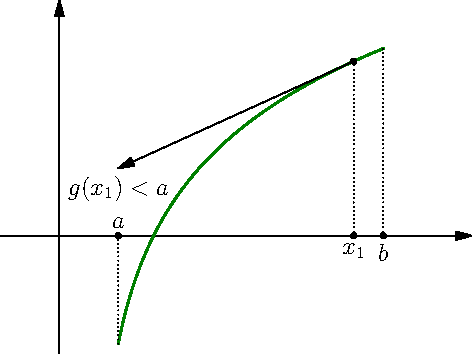
\includegraphics{./Cnewton_1.pdf}
  % Cnewton_1.pdf: 128x170 pixel, 72dpi, 4.52x6.00 cm, bb=0 0 128 170
  \caption{II.3.a. Exemple de graphe de $f$}
  \label{fig:Cnewton_1}
\end{figure}

\item \begin{enumerate}
 \item La restriction de $\ln$ à un segment de $]0,+\infty[$ satisfait aux conditions. Dans la Figure \ref{fig:Cnewton_1} on a tracé un graphe de ce genre.
 \item Remarquons que l'intervalle $[a,b]$ complet \emph{n'est pas stable}. On a indiqué sur la figure \ref{fig:Cnewton_1} un point $x_1$ dont l'image n'est pas dans $[a,b]$.\newline
 Montrons que l'intervalle $[a,\alpha]$ est stable.\newline
 Montrons d'abord que la restriction de $g$ est croissante. En effet:
\[
 g'(x) = \frac{f(x)f''(x)}{f'(x)^2} > 0
\]
car $f''$ est négative partout et $f(x)< 0$ dans $[a,\alpha[$. D'autre part $g(\alpha) > \alpha$ car $f(\alpha)<0$ donc 
\[
 g(\left[ a, \alpha\right]) = \left[ g(a), g(\alpha)\right] =   \left[ g(a), \alpha\right] \subset  \left[ a, \alpha\right].   
\]
On peut aussi remarquer (calcul de $g'$) que, dans $[a,\alpha]$, $g$ est croissante et telle que $g(x)\geq x$. On en déduit que $[a,\alpha]$ est stable pour $g$.

\item D'après $b$, comme la restriction de $g$ est croissante, l'inégalité $x_0 < x_1$ se propage ce qui montre que la suite $(x_n)_{n\in\N}$ est croissante. Elle est majorée par $\alpha$. Elle est donc convergente. Sa limite notée $\beta$ est un élément de $[a,\alpha]$, la fonction $g$ est continue en $\beta$ et la définition de $x_n$ entraîne alors $g(\beta)=\beta$. Or par définition de $g$, un point fixe de $g$ est un zéro de $f$ et $\alpha$ est le seul zéro de $f$ dans $I$.\\
On peut donc conclure que $(x_n)_{n\in\N}$ converge vers $\alpha$.
\end{enumerate}
\item
\begin{enumerate}
 \item Comme $g'$ est continue en $\alpha$ et $g'(\alpha)=0$, il existe un intervalle $J$ de la forme $[\alpha-h,\alpha+h]$ tel que $|g'(x)|<1$ pour tout $x\in J$.
\item Pour tous les $x\in J$, appliquons le théorème des accroissements finis à $g$ entre $x$ et $\alpha$. Il existe donc $c_x$ entre $x$ et $\alpha$ tel que
\begin{displaymath}
 |g(x)-\alpha| = |g(x)-g(\alpha)| = |x-\alpha||g'(c_x)|<|x-\alpha|
\end{displaymath}
 ce qui entraîne que $g(x)$ est encore entre $x$ et $\alpha$ donc dans $J$.
\item L'intervalle $J$ est un segment et la fonction $|g'|$ est continue sur cet intervalle. Elle est donc bornée et elle atteint sa borne supérieure $M$ en un point de $J$. Il existe $u\in J$ tel que $M=|g'(u)|<1$ d'après la définition de $J$. L'inégalité des accroissements finis appliquée entre deux éléments quelconques de $J$ montre que $g_{|J}$ est $M$-lipschitzienne.
\item Toutes les hypothèses sont maintenant réunies pour appliquer à $g$ dans $J$ les résultats de la partie $I$. La suite $(x_n)_{n\in \N}$ converge vers l'unique point fixe $\alpha$ de $g$.
\end{enumerate}

\end{enumerate}
%
\newpage%
\section*{Problème 32}%
\addcontentsline{toc}{section}{Pb 32 : Opérateur intégral.}%
\fancyhead[LO,RE]{Corrigés - Pb 32 : Opérateur intégral.}%
\begin{enumerate}
 \item Les ensembles $E$ et $F$ sont des $\R$-espaces vectoriels à cause des propriétés usuelles de linéarité de la continuité et de la dérivabilité. 
\item Si $f$ est dans $E=C^0(\R,\R)$, pourquoi $\phi_f$ est-elle dans $F$? On doit vérifier les propriétés caractéristiques des fonctions de $F$.\newline
Par définition, $\phi_f$ est la primitive de $t\rightarrow tf(t)$ nulle en $0$. C'est donc bien une fonction $\mathcal C^1$ nulle en $0$ et à dérivée nulle en $0$. Sa dérivée est dérivable en $0$ car, en $0$, 
\begin{displaymath}
 \phi_f'(x) = xf(x) = x(f(0)+o(1)) = f(0)x + o(x) \Rightarrow \phi_f'' = f(0)
\end{displaymath}
La fonction $\phi$ est linéaire à cause de la linéarité de l'intégration.

\item Pour montrer que $f$ est dans $E$, on doit montrer qu'elle est continue.\newline
Par définition et opérations usuelles, elle clairement continue en un point quelconque autre que $0$. La continuité de $f$ en $0$ traduit la dérivabilité de $g'$ en $0$ (avec $g'(0)=0$).\newline
Pour une fonction $f$ ainsi définie:
\begin{displaymath}
 \phi_f(x)=\int_{0}^{x}t\, \frac{g'(t)}{t}dt = \left[ g\right]_{0}^{x} =g(x)
\end{displaymath}
La fonction $f$ est donc un antécédent de $g$. Comme  $g$ est quelconque dans $F$, ceci montre que la fonction $\phi$ est surjective.
\item Pour montrer que $\Phi$ est un isomorphisme, il reste à montrer l'injectivité. C'està dire que le noyau se réduit à la fonction nulle. Soit donc $f\in\ker \phi$
\begin{displaymath}
 \forall x\in\R : \int_{0}^{x}tf(t)dt = 0
\end{displaymath}
 En dérivant, on obtient :
\begin{displaymath}
 \forall x\in\R : xf(x)=0
\end{displaymath}
On en déduit $f(x)=0$ pour tous les $x$ \emph{non nuls}. On obtient $f(0)=0$ par continuité de $f$ en $0$.
\end{enumerate}
%
\newpage%
\section*{Problème 33}%
\addcontentsline{toc}{section}{Pb 33 : Polynômes et suites. Limite de la suite des 1/k^2}%
\fancyhead[LO,RE]{Corrigés - Pb 33 : Polynômes et suites. Limite de la suite des 1/k^2}%
\begin{enumerate}
\item \begin{enumerate}
 \item En {\'e}crivant les deux termes de plus haut degr{\'e} de la formule du bin{\^o}me, on montre que $Q_{n}$ est de degr{\'e} $n$ et de coefficient dominant $n+1$.
\item En substituant $-X$ à $X$ dans $Q_n$ on obtient $(-1)^{n}Q_n$. On en déduit que $Q_n$ est de même parité que $n$ et que l'ensemble des racines de $Q_n$ est symétrique (si $z$ est racine alors $-z$ l'est aussi).
      \end{enumerate}

\item  \'Ecrivons cette fois la formule compl{\`e}te :
\[
Q_{2r}=\frac{1}{2i}\sum_{k=0}^{2r+1}\binom{2r+1}{k}\left( 1-(-1)^{k}\right).
(i)^{k}X^{2r+1-k}
\]
De plus $1-(-1)^{k}$ est nul si $k$ est pair, il vaut 2 si $k$ est impair. Les entiers impairs $k$ entre $1$ et $2r+1$ sont de la forme $2p+1$ avec $p\in \llbracket 0, r\rrbracket$. Alors $i^{k}=(-1)^{p}i$ d'où
\[
Q_{2r}=\sum_{p=0}^{r}\binom{2r+1}{2p+1}(-1)^{p}X^{2(r-p)}.
\]
 On retrouve bien le fait que $Q_{2r}$ est pair. Il est clair que
\[
S_{r}=\sum_{p=0}^{r}\binom{2r+1}{2p+1}(-1)^{p}X^{r-p}.
\]
  
\item  Les racines de $Q_{n}$ sont les complexes $z$ tels que 
\begin{displaymath}
(z+i)^{n+1}=(z-i)^{n+1} .
\end{displaymath}
Comme $i$ n'est pas solution de cette {\'e}quation, celle ci est {\'e}quivalente {\`a} 
\begin{displaymath}
\left( \frac{z+i}{z-i}\right) ^{n+1}=1 \Leftrightarrow \frac{z+i}{z-i} \in \U_{n+1} \setminus \left\lbrace 1 \right\rbrace.
\end{displaymath}
Il convient d'enlever $1$ car $ \frac{z+i}{z-i}\neq 1$ pour tout $z \in \C$. On en déduit que $z$ est une racine si et seulement si
\begin{displaymath}
\exists k \in \llbracket 1,n \rrbracket \text{ tq } \frac{z+i}{z-i}=e^{\frac{2ik\pi }{n+1}} .
\end{displaymath}
Il faut exclure $k=0$ car $\frac{z+i}{z-i}$ est toujours diff{\'e}rent de 1.\newline
En transformant la relation (homographique) précédente, on obtient que $z$ est racine si et seulement si 
\[
\exists k \in \llbracket 1,n \rrbracket \text{ tq }  z = -i\,\frac{1+e^{\frac{2ik\pi }{n+1}}}{1-e^{\frac{2ik\pi }{n+1}}}
= -i\, \frac{2\cos \frac{k\pi }{n+1}}{-2i\sin \frac{k\pi }{n+1}}
= \cot \frac{k\pi }{n+1}.
\]
Ces racines sont distinctes car l'application\footnote{une telle application est dite homographiqe} $z\rightarrow \frac{z+i}{z-i}$ est bijective de $\C-\{i\}$ dans $\C-\{1\}$. 
Avec le coefficient dominant, l'expression des racines conduit {\`a} la factorisation
\[
Q_{n}=(n+1)\prod_{k=1}^{n}\left( X-\cot \frac{k\pi }{n+1}\right).
\]

\item  Lorsque $k\in \llbracket 1,r\rrbracket$, l'entier $2r+1-k$
d{\'e}crit $\rrbracket r+1,2r\rrbracket$ avec
\[
\cot \frac{(2r+1-k)\pi }{2r+1}=\cot (\pi -\frac{k\pi }{2r+1})=-\cot \frac{k\pi }{2r+1}.
\]
Pour tout $k\in\llbracket 1 ,r\rrbracket$, on regroupe les racines opposées associ{\'e}es {\`a} $k$ et {\`a} $2r+1-k$. On obtient
\[
Q_{2r}=(2r+1)\prod_{k=1}^{r}\left( X^{2}-\cot ^{2}\frac{k\pi }{2r+1}\right).
\]
En d{\'e}veloppant, il apparait que le coefficient du terme de degr{\'e} $2r-2$ de $Q_{2r}$ est
\[
-(2r+1)\sum_{k=1}^{r}\cot ^{2}\frac{k\pi }{2r+1}.
\]
D'autre part, l'expression de $S_r$, ce coefficient est aussi
\[
-\binom{2r+1}{3}=-\frac{(2r+1)(2r)(2r-1)}{6}.
\]
On en d{\'e}duit
\[
\sum_{k=1}^{r}\cot ^{2}\frac{k\pi }{2r+1}=\frac{r(2r-1)}{3}.
\]
En rempla\c{c}ant $\cot ^{2}$ par$\frac{1}{\sin ^{2}}-1$ dans la formule pr{\'e}c{\'e}dente, il vient
\[
\sum_{k=1}^{r}\frac{1}{\sin ^{2}\frac{k\pi }{2r+1}} = r + \frac{r(2r-1)}{3}
= \frac{2r(r+1)}{3}.
\]

\item  Dans $\left] 0,\frac{\pi }{2}\right[ $, $\sin $ et $\cot $ sont strictement positifs. Les in{\'e}galit{\'e}s demand{\'e}es se déduisent donc de $\sin x<x<\tan x$. Celles ci se d{\'e}montrent tr{\`e}s rapidement en formant les tableaux de variation de $x-\sin x$ et de
$\tan x-x$.

\item  \'Ecrivons les inégalités de la question précédente avec $x=\frac{k\pi }{2r+1} \in \left] 0,\frac{\pi }{2}\right[$ pour tous les $k\in \llbracket 1,r\llbracket$  et additionnons les en tenant compte de 4. Il vient
\[
\frac{r(2r-1)}{3}
\leq \sum_{k=1}^{r}\frac{1}{\left( \frac{k\pi }{2r+1}\right) ^{2}}
\leq \frac{2r(r+1)}{3}.
\]

\item  L'encadrement pr{\'e}c{\'e}dent s'{\'e}crit encore
\begin{align*}
\left( \frac{\pi }{2r+1}\right) ^{2}\frac{r(2r-1)}{3} 
&\leq 
\sum_{k=1}^{r}\frac{1}{k^{2}}\leq \left( \frac{\pi }{2r+1}\right) ^{2}\frac{2r(r+1)}{3} \\
\frac{\pi^{2}}{3}\frac{r(2r-1)}{(2r+1)^{2}} 
&\leq 
\sum_{k=1}^{r}\frac{1}{k^{2}}\leq \frac{2\pi ^{2}}{3}\frac{r(r+1)}{(2r+1)^{2}}.
\end{align*}
Quand $r\rightarrow +\infty $, les suites {\`a} droite et {\`a} gauche convergent vers $\frac{\pi ^{2}}{6}$. On en d{\'e}duit
\[
(\sum_{k=1}^{r}\frac{1}{k^{2}})_{r\in \mathbf{N}}\rightarrow \frac{\pi ^{2}}{6}.
\]
\end{enumerate}
%
\newpage%
\section*{Problème 34}%
\addcontentsline{toc}{section}{Pb 34 : Relations entre coefficients et racines, éléments simples.}%
\fancyhead[LO,RE]{Corrigés - Pb 34 : Relations entre coefficients et racines, éléments simples.}%
\begin{enumerate}
\item Comme $\tilde{A}(0)=0$, le polynôme $A$ est divisible par $X$. Il existe donc un polynôme $B$ tel que $A=XB$. Ce polynôme est de degré $2n-1$ et de coefficient dominant 1. On peut obtenir le terme de degré 0 à partir de la dérivée.
\[A'=2n(X+1)^{2n-1}=XB'+B,\quad\tilde{A'}(0)=\tilde{B}(0)=2n\]
\item Les racines de $A$ sont les nombres complexes $u-1$ où $u$ décrit l'ensemble $\U_{2n}$ des racines $2n$ ièmes de l'unité.
\item Lorsque $k$ décrit $\llbracket 1, n-1 \rrbracket$, le nombre $2n-k$ décrit $\llbracket n+1, 2n-1\rrbracket$.
\[
\frac{(2n-k)\pi}{2n}=\pi-\frac{k\pi}{2n}
\Rightarrow
\sin\frac{(2n-k)\pi}{2n}=\sin \frac{k\pi}{2n} .
\]
On en déduit 
\[
P_{n}=\prod_{k=n+1}^{2n-1}\sin \frac{k\pi}{2n}
\]
puis $Q_{n}=P_{n}^{2}$ car, pour $k=n$, $\sin \frac{k\pi}{2n}=1$.\newline
Comme tous les $\frac{k\pi}{2n}$ sont dans $[0,\frac{\pi}{2}]$, les $\sin$ sont positifs et $P_{n}=\sqrt{Q_{n}}$.

\item Les racines non nulles de $A$ sont les racines de $B$. Notons $E$ le produit de ces $2n-1$ racines. En développant l'expression factorisée du polynôme et en identifiant, il vient 
\[
E = (-1)^{2n-1}\frac{b_{0}}{b_{2n-1}} = -2n
\]
En formant directement le produit des racines, il vient $E = \prod_{u\in \U_{2n}-\{1\}}(u-1)$. Chaque $u$ de $\U_{2n}-\{1\}$ est de la forme $e^{i\theta}$ avec $\theta=\frac{k\pi}{n}$ et $k\in \llbracket 1, 2n-1\rrbracket$. D'où
\begin{multline*}
E = (2i)^{2n-1}e^{i\sum_{k=1}^{2n-1}\frac{k\pi}{n}}\prod_{k=1}^{2n - 1}\sin \frac{k\pi}{n} \text{ avec }
e^{i\sum_{k=1}^{2n-1}\frac{k\pi}{n}} = e^{i(2n-1)\frac{\pi}{2}}=(i)^{2n-1}\\
\Rightarrow E = 2^{2n-1}(-1)^{2n-1}Q_{n}=-2^{2n-1}Q_{n}.
\end{multline*}
Finalement $Q_{n}=n\,2^{-2n+2}$,$P_{n}=\sqrt{n}\,2^{-n+1}$.
\item La décomposition de $F$ en éléments simples est de la forme
\[
\sum _{u\in \U_{2n}}\frac{\lambda(u)}{X-u+1}
 \text{ avec }
\lambda(u)=\frac{1}{\tilde{A'}(u-1)}=\frac{1}{2nu^{2n-1}}=\frac{u}{2n}. 
 \]
\end{enumerate}
%
\newpage%
\section*{Problème 35}%
\addcontentsline{toc}{section}{Pb 35 : Condition polynomiale}%
\fancyhead[LO,RE]{Corrigés - Pb 35 : Condition polynomiale}%
\begin{enumerate}
 \item Si $P=\lambda\in \C$, la condition devient $\lambda=\lambda^2$. Dans $\C_0[X]$, les solutions sont $0$ et $1$.

 \item 
\begin{enumerate} 
\item Définissons une fonction $f$ par $f(x)=x^2+2x$. Elle est strictement croissante dans $[0,+\infty[$. La suite $\left( a_n\right) _{n\in \N}$ est donc monotone. De plus $f(x)-x=x(x+1)>0$ pour $x>0$ et $0, -1$ sont les seuls points fixes de $f$. On en déduit que $a_0<a_1$. Cette inégalité se propage par $f$, la suite est strictement croissante. Si elle convergeait, ce serait vers un point fixe de $f$. Or il n'en existe pas dans $]0,+\infty[$, la suite diverge donc vers $+\infty$. Décrivons tous les comportements possibles.
\begin{itemize}
 \item Si $a_0>0$, la suite croît strictement vers $+\infty$.
 \item Si $a_0<-2$ alors $a_1>0$ car $f(x)=x(x+2)$. On est donc ramené au premier cas et le suite diverge ensuite vers $+\infty$.
 \item Si $a_0\in]-1,0[$ alors la suite converge en décroissant vers $-1$. En effet l'intervalle $[-1,0]$ est stable et la fonction y est croissante. La suite est monotone, décroissante car $a_1-a_0=a_0(a_0-1)<0$ minorée par $-1$. Elle converge vers le seul point fixe possible soit $-1$.
 \item Si $a_0=0$ la suite est constante de valeur $0$. 
 \item Si $a_0=-$ la suite est constante de valeur $-1$.
 \item Si $a_0=-2$ alors $a_1=0$ et la suite garde la valeur $0$ pour les autres indices.
 \item Si $a_0\in]-2,-1[$ alors $a_1\in]-1,0[$, on est ramené au troisième cas, la suite décroît ensuite vers $-1$.
\end{itemize}
 \item D'après la relation de récurrence
\begin{displaymath}
 a_{n+1}+1=a_n^2+2a_n+1=(a_n+1)^2
\end{displaymath}
On en déduit
\begin{displaymath}
 a_1+1=(a_0+1)^2 \rightarrow a_2+1=(a_1+1)^2=(a_0+1)^4 \rightarrow \cdots
\end{displaymath}
On vérifie par récurrence
\begin{displaymath}
 a_n +1 = (a_0+1)^{(2^n)}
\end{displaymath}
Remarquons que la suite complexe $\left( a_n+1\right) _{n\in \N}$ est \emph{extraite} de la suite géométrique de raison $a_0+1$ avec des exposants égaux à des puissances de $2$. On peut donc discuter de son comportement.
\begin{itemize}
 \item Si $|a_0+1|<1$, la suite $\left(a_n+1 \right) _{n\in \N}\rightarrow 0$ donc $\left(a_n \right) _{n\in \N}\rightarrow -1$.
 \item Si $|a_0+1|>1$, $\left(|a_n+1 |\right) _{n\in \N}\rightarrow +\infty$ donc $\left(a_n \right) _{n\in \N}$ ne converge pas vers $-1$.
 \item Si $|a_0+1|=1$, $\left(|a_n+1 |\right) _{n\in \N}$ est constante de valeur $1$ donc $\left(a_n \right) _{n\in \N}$ ne converge pas vers $-1$.
\end{itemize}
On en déduit que le bassin d'attraction de $-1$ est le disque ouvert centré en $-1$ et de rayon $1$.
\end{enumerate}

 \item Substituons $a+1$ à $X$ dans la relation $(*)$. On obtient
\begin{displaymath}
 \widetilde{P}((a+1)^2-1)=\widetilde{P}(a)\widetilde{P}(a+2)
\end{displaymath}
donc $a$ racine de $P$ entraine $(a+1)^2-1$ racine de $P$. On en tire que, si $a_0$ est racine de $P$, alors toutes les valeurs $a_n$ de la suite sont aussi des racines de $P$.

 \item
\begin{enumerate}
 \item Si $P$ admettait une racine $a>0$, en posant $a_0=a$, on obtiendrait que toutes les valeurs $a_n$ de la suite seraient aussi des racines. Or elles sont deux à deux distinctes car la suite est strictement croissante dans ce cas. Ceci est contradictoire avec le fait que $P$ ne peut admettre qu'un nombre fini (inférieur ou égal à son degré) de racines.
 \item En substituant $-2$ à $X$ dans $(*)$, on obtient $\widetilde{P}(3)=\widetilde{P}(-3)\widetilde{P}(-1)$.\newline
Si $-1$ était racine, $3$ le serait aussi ce qui est impossible d'après le a. On en conclut que  $-1$ n'est pas racine de $P$.
 \item Si $a$ est une racine complexe, alors toutes les valeurs de la suite $\left( a_n\right) _{n\in \N}$ définie par $a_0=a$ sont aussi des racines. L'ensemble des racines est fini, l'application $n\mapsto a_n$ n'est donc pas injective. Il existe des entiers $n<p$ tels que
\begin{displaymath}
 (a+1)^{2^n}=(a+1)^{2^p}
\end{displaymath}
En simplifiant par $(a+1)^{2^n}\neq 0$, on obtient
\begin{displaymath}
 1=(a+1)^{2^p-2^n} \Rightarrow |a+1| = 1
\end{displaymath}
\end{enumerate}

 \item En substituant $a-1$ à $X$ dans $(*)$, on obtient
\begin{displaymath}
 \widetilde{P}((a-1)^2-1)=\widetilde{P}(a-2)\widetilde{P}(a)
\end{displaymath}
On en déduit que $a$ racine de $P$ entraine $(a-1)^2-1$ racine de $P$. D'après la question 4.c on peur écrire 
\begin{displaymath}
|\left( (a-1)^2-1\right) -1|=1 \Rightarrow |a-1| = 1
\end{displaymath}

 \item D'après les questions précédentes, si $P$ est de degré au moins $1$ et vérifie la relation, toute racine complexe $a$ de $P$ doit se trouver sur les deux cercles de rayon 1 centrés en $-1$ ou en $-1$. Le seul $a$ possible est $0$. On en déduit que les polynômes vérifiant $(*)$ sont seulement $0,1$ et les $X^n$ avec $n\in \N^*$. La vérification qu'ils satisfont effectivement à la relation est immédiate, elle revient à l'identité
\begin{displaymath}
 (X^2-1)^n = (X-1)^2(X+1)^n
\end{displaymath}

\end{enumerate}
%
\newpage%
\section*{Problème 36}%
\addcontentsline{toc}{section}{Pb 36 : Un problème sur des rotations vectorielles.}%
\fancyhead[LO,RE]{Corrigés - Pb 36 : Un problème sur des rotations vectorielles.}%
\subsection*{Préambule}
\begin{enumerate}
 \item On forme le tableau de variations de la fonction polynomiale :
\begin{displaymath}
\begin{array}{|ccccccc|}
-\infty &          & 0      &         & \frac{2}{3} &         & +\infty \\  \hline
        &          & \mu    &         &             &         & +\infty \\ 
        & \nearrow &        &\searrow &             &\nearrow &          \\
-\infty &          &        &         & \mu-\frac{4}{27}            &         &          \\ \hline
\end{array}
 \end{displaymath}
Cette fonction prend trois fois la valeur $0$ si et seulement si $\mu$ est strictement positif et $\mu -\frac{4}{27}$ strictement négatif. La condition demandée est donc
\begin{displaymath}
 \mu \in \left] 0, \dfrac{4}{27}\right[ 
\end{displaymath}
\item Les racines doubles sont à chercher parmi les racines de la dérivée. Les seules possibilités sont les suivantes
\begin{description}
 \item $0$ est racine double si et seulement si $\mu=0$. L'autre racine est alors $1$.
\item $\dfrac{2}{3}$ est racine double si et seulement si $\mu=\dfrac{4}{27}$. L'autre racine est alors $-\dfrac{1}{3}$.
\end{description}
\end{enumerate}

\subsection*{Partie I}
\begin{enumerate}
 \item L'application $f_\lambda$ est clairement à valeurs dans $E$. Elle est linéaire car le produit scalaire est bilinéaire.

 \item \begin{enumerate}
 \item D'après le cours, $f_\lambda$ est un automorphisme lorsqu'il conserve la distance. C'est à dire
\begin{displaymath}
 \forall \overrightarrow x \in E :  
\Vert f_\lambda(\overrightarrow x)\Vert^2 = \Vert \overrightarrow x \Vert^2
\end{displaymath}

Or :
\begin{displaymath}
 \Vert f_\lambda(\overrightarrow x)\Vert^2 = 
\Vert \overrightarrow x \Vert^2 + \lambda^2 <\overrightarrow x, \overrightarrow u>^2 + 2\lambda <\overrightarrow x, \overrightarrow u>^2
\end{displaymath}
Donc
\begin{displaymath}
 \Vert f_\lambda(\overrightarrow x)\Vert^2 = \Vert \overrightarrow x \Vert^2 \Leftrightarrow
\lambda <\overrightarrow x, \overrightarrow u>^2 \left(\lambda + 2\right) =0
\end{displaymath}
Ceci se produit (pour tous les $\overrightarrow x$) lorsque $0$ ou $-2$. La valeur $0$ conduit à l'identité. On en déduit
\begin{displaymath}
 \lambda_0 = -2
\end{displaymath}

\item Si la matrice des coordonnées de $\overrightarrow x$ dans $\mathcal B$ est 
\begin{displaymath}
 \begin{pmatrix}
  x \\ y \\ z
 \end{pmatrix}
\end{displaymath}
celle de $f_{-2}(\overrightarrow x)$ est 
\begin{displaymath}
 \begin{pmatrix}
  x \\ y \\ z
 \end{pmatrix} 
-2(ax+by+cz)
\begin{pmatrix}
  a \\ b \\ c
 \end{pmatrix}
\end{displaymath}
On ne déduit la matrice cherchée :
\begin{displaymath}
 \Mat_{\mathcal B}f_{-2}=
\begin{pmatrix}
 1-2a^2 & -2ab & -2ac \\
-2ab & 1-2b^2 & -2bc \\
-2ac & -2bc &1-2c^2
\end{pmatrix}
\end{displaymath}
\item Un vecteur $\overrightarrow x$ est invariant par $f_{-2}$ si et seulement si $<\overrightarrow x , \overrightarrow u>=0$. L'ensemble des vecteurs invariants est donc l'hyperplan $(\Vect \overrightarrow x)^\perp$. L'automorphisme $f_{-2}$ est la symétrie orthogonale (réflexion) par rapport à ce plan.
\end{enumerate}
\end{enumerate}

\subsection*{Partie II}
\begin{enumerate}
 \item L'endomorphisme $g$ est une rotation vectorielle si et seulement si sa matrice $G$ est orthogonale et de déterminant $1$. Ce qui, après calcul du produit et du déterminant, se traduit par :
\begin{displaymath}
 \left\lbrace 
\begin{aligned}
 \mathstrut^t\! G\,G &= I_3 \\
\det G &= 1
\end{aligned}
\right. 
\Leftrightarrow
\left\lbrace 
\begin{aligned}
 a^2+b^2+c^2 &= 1 \\
ac +ab+bc &= 0 \\
a^3 + b^3 + c^3 -3abc &= 1
\end{aligned}
\right. 
\end{displaymath}
L'énoncé nous signale l'identité
\begin{displaymath}
 a^3 + b^3 + c^3 -3abc = (a+b+c)\left( (a^2+b^2+c^2)-(ab+bc+ac)\right) 
\end{displaymath}
On peut donc former d'autres systèmes équivalents au premier :
\begin{displaymath}
 \left\lbrace 
\begin{aligned}
  a^2+b^2+c^2 &= 1 \\
ac +ab+bc &= 0 \\
a+b+c &= 1
\end{aligned}
\right. 
\Leftrightarrow
\left\lbrace 
\begin{aligned}
ac +ab+bc &= 0 \\
a+b+c &= 1
\end{aligned}
\right. 
\end{displaymath}
car $a^2+b^2+c^2=(a+b+c)^2-2(ac+ab+bc)$.\newline
Lorsque $g$ est une rotation, $(a,b,c)$ sont les trois racines réelles du polynôme réel 
\begin{displaymath}
 (x-a)(x-b)x-c)= x^3 -(a+b+c)x^2+(ab+ac+bc)x-abc=x^3-x^2+p
\end{displaymath}
pour $p=-abc$. D'après le préambule, ce polynôme admettant trois racines réelles on doit avoir $p\in ]0,\frac{4}{27}[$.\newline
Réciproquement, si $p\in ]0,\frac{4}{27}[$, les trois racines $a$, $b$, $c$ du polynôme $x^3-x^2-p$ vérifient
\begin{displaymath}
 \left\lbrace 
\begin{aligned}
ac +ab+bc &= 0 \\
a+b+c &= 1
\end{aligned}
\right. 
\end{displaymath}
et définissent donc une rotation $g$.
\item Lorsque $g$ est une rotation avec $b=c$, on se retrouve dans le cadre des racines doubles de la question 2. du préambule.
\begin{itemize}
 \item Si $b=c=0$ et $a=0$ alors $g$ est l'identité.
\item Si $b=c=\frac{2}{3}$  et $a=-\frac{1}{3}$ alors la matrice de $g$ dans une base orthonormée est à la fois symétrique et orthogonale. C'est donc (cours) la matrice d'une symétrie orthogonale directe. C'est une symétrie par rapport à une droite (demi-tour) ou encore une rotation d'angle $\pi$. Après résolution d'un système linéaire, on trouve que l'axe est dirigé par un vecteur de coordonnées
\begin{displaymath}
 \begin{bmatrix}
  1 \\ 1 \\ 1
 \end{bmatrix}
\end{displaymath}
Remarque. Pour un angle $\pi$, l'orientation de l'axe est sans importance.
\end{itemize}
\end{enumerate}

\subsection*{Partie III}
\begin{figure}[ht]
 \centering
 \input{Crot_1.pdf_t}
 \caption{Décomposition orthogonale pour la question III.1.}
\end{figure}
\begin{enumerate}
 \item Le produit scalaire et le produit vectoriel permettent d'exprimer \emph{explicitement} la décomposition orthogonale d'un vecteur $\overrightarrow x$ dans $\Vect \overrightarrow u$ et $(\Vect \overrightarrow u)^\perp$
\begin{displaymath}
 \overrightarrow x =
<\overrightarrow u , \overrightarrow x> \overrightarrow u +
(\overrightarrow u \wedge \overrightarrow x)\overrightarrow u 
\end{displaymath}
Pour montrer cette formule, notons $\overrightarrow y$ le projeté orthogonal de $x$ sur $(\Vect \overrightarrow u)^\perp$. Alors:
\begin{multline*}
\overrightarrow x =
<\overrightarrow u , \overrightarrow x> \overrightarrow u + \overrightarrow y
\Rightarrow (\overrightarrow u \wedge \overrightarrow x) = \overrightarrow u \wedge \overrightarrow y \\
 \Rightarrow
(\overrightarrow u \wedge \overrightarrow x)\wedge \overrightarrow u 
=
(\overrightarrow u \wedge \overrightarrow y)\wedge \overrightarrow u 
= \Vert \overrightarrow u \Vert^2 \overrightarrow y - <\overrightarrow y, \overrightarrow u> \overrightarrow u
=\overrightarrow y 
\end{multline*}
De plus, la famille 
$\left(
(\overrightarrow u \wedge \overrightarrow x)\wedge \overrightarrow u,
\overrightarrow u \wedge \overrightarrow x,
\overrightarrow u
 \right) $
est une base ortogonale directe dont le premier vecteur est le projeté ortogonal de $\overrightarrow x$. On en déduit l'effet d'une rotation d'angle $\theta$ autour de $\overrightarrow u$:
\begin{displaymath}
 r(\overrightarrow{x})
    =<\overrightarrow{x},\overrightarrow{u}> \overrightarrow{u}
     + \cos \theta \,(\overrightarrow{u}\wedge\overrightarrow{x})\wedge \overrightarrow{u}
     + \sin \theta \,(\overrightarrow{u}\wedge\overrightarrow{x})
\end{displaymath}
Remarque. La base orthogonale est directe car :
\begin{multline*}
 \det
\left( 
(\overrightarrow u \wedge \overrightarrow x)\wedge \overrightarrow u,
\overrightarrow u \wedge \overrightarrow x,
\overrightarrow u
\right) 
=
 \det
\left( 
\overrightarrow u \wedge \overrightarrow x,
\overrightarrow u,
(\overrightarrow u \wedge \overrightarrow x)\wedge \overrightarrow u
\right) \\
=
\left\Vert
(\overrightarrow u \wedge \overrightarrow x)\wedge \overrightarrow u
\right\Vert ^2
>0
\end{multline*}
On peut former une base orthonormée directe:
\begin{displaymath}
 \left( 
\dfrac{1}{\Vert \overrightarrow u \wedge \overrightarrow x\Vert}(\overrightarrow u \wedge \overrightarrow x)\wedge \overrightarrow u,
\dfrac{1}{\Vert \overrightarrow u \wedge \overrightarrow x\Vert} \overrightarrow u \wedge \overrightarrow x,
\overrightarrow u
\right) 
\end{displaymath}
\item D'après la démonstration de la question précédente, il est évident que la formule définit une rotation vectorielle d'angle $\theta$ autour de $\overrightarrow u$.
\item La matrice $\Phi$ de $\varphi$ se décompose en $S+A$ avec :
\begin{align*}
 A =
\begin{pmatrix}
a^2 & ab & ac \\
ab & b^2 & bc \\
ac & bc &c^2
 \end{pmatrix}
& &
S=
\begin{pmatrix}
0 & -c & b \\
c & 0 & -a \\
-b & a 0
\end{pmatrix}
\end{align*}
Chacune de ces matrices peut s'interpréter. Considérons un vecteur $\overrightarrow u$ de coordonnées $(a,b,c)$ dans la base $\mathcal B$.\newline
La matrice de $\overrightarrow x \rightarrow <\overrightarrow x , \overrightarrow u>\overrightarrow u$ dans $\mathcal B$ est $S$. En effet :
\begin{displaymath}
\left(ax+by+cz \right) 
 \begin{pmatrix}
  a \\ b \\ c
 \end{pmatrix}
=
\begin{pmatrix}
 a^2x+aby+acz \\
abx+b^2y+bcz \\
acx+bcy+c^2z
\end{pmatrix}
=
\begin{pmatrix}
a^2 & ab & ac \\
ab & b^2 & bc \\
ac & bc &c^2
 \end{pmatrix}
\begin{pmatrix}
 x \\ y \\ z
\end{pmatrix}
\end{displaymath}
La matrice de $\overrightarrow x \rightarrow \overrightarrow x \wedge \overrightarrow u$ dans $\mathcal B$ est $A$. En effet :
\begin{displaymath}
 \begin{pmatrix}
  a \\ b \\ c
 \end{pmatrix}
\wedge
\begin{pmatrix}
 x \\ y \\ z
\end{pmatrix}
=
\begin{pmatrix}
bz-cy\\
cx-az\\
ay-bx 
\end{pmatrix}
=
\begin{pmatrix}
0 & -c & b \\
c & 0 & -a \\
-b & a & 0
\end{pmatrix}
\begin{pmatrix}
 x \\ y \\ z
\end{pmatrix}
\end{displaymath}
On pourrait aussi considérer la matrice $Z$ de $\overrightarrow x \rightarrow (\overrightarrow x \wedge \overrightarrow u)\wedge \overrightarrow u$ mais en fait il est inutile de la calculer. Il suffit de remarquer que 
\begin{displaymath}
 \Phi = S + A = S + \cos \dfrac{\pi}{2} Z + \sin \dfrac{\pi}{2} A
\end{displaymath}
On en déduit que $\varphi$ est la rotation d'angle $\dfrac{\pi}{2}$ autour de $\overrightarrow u$
\item \begin{enumerate}
\item D'après III.1. l'expression du retournement est
\begin{displaymath}
 \overrightarrow x \rightarrow 
<\overrightarrow{x},\overrightarrow{u}> \overrightarrow{u}
     + \cos \pi (\overrightarrow{u}\wedge\overrightarrow{x})\wedge \overrightarrow{u}
     + \sin \pi (\overrightarrow{u}\wedge\overrightarrow{x})
=
<\overrightarrow{x},\overrightarrow{u}> \overrightarrow{u} - 
(\overrightarrow{u}\wedge\overrightarrow{x})\wedge \overrightarrow{u}
\end{displaymath}
 \item D'après la question précédente, la matrice  du demi-tour est $S-Z$. On a donc besoin ici de calculer la matrice $Z$ de $\overrightarrow x \rightarrow (\overrightarrow x \wedge \overrightarrow u)\wedge \overrightarrow u$.
\begin{displaymath}
\begin{pmatrix}
bz-cy\\
cx-az\\
ay-bx 
\end{pmatrix}
\wedge
\begin{pmatrix}
  a \\ b \\ c
\end{pmatrix}
=
\begin{pmatrix}
 (c^2+b^2)x-aby-acz \\
-abx +(a^2+c^2)y -bcz \\
-acx -bcy +(a^2+b^2)z
\end{pmatrix}
\end{displaymath}
 On en déduit la matrice $Z$:
\begin{displaymath}
 Z=
\begin{pmatrix}
 c^2+b^2 & -ab & -ac \\
-ab & a^2+c^2 & -bc \\
-ac & -bc & a^2+b^2
\end{pmatrix}
\end{displaymath}
puis la matrice cherchée qui est égale à $S-Z$ soit
\begin{displaymath}
 \begin{pmatrix}
a^2-c^2+b^2 & 2ab & 2ac \\
2ab & -a^2+b^2-c^2 & 2bc \\
2ac & 2bc & -a^2-b^2c^2
 \end{pmatrix}
\end{displaymath}
\end{enumerate}

\end{enumerate}
\subsection*{Partie IV}
Dans cette partie, $r$ est la rotation d'angle $\theta$ autour de $\overrightarrow u$, la réflexion de plan $(\Vect(\overrightarrow u))^\perp$ est notée $s$ et $\delta$ est la composée $s\circ r$. L'automorphisme orthogonal $\delta$ est donc une rotation-miroir.
\begin{enumerate}
 \item La matrice de $\delta$ dans une base orthonormée directe $(\overrightarrow a , \overrightarrow b , \overrightarrow u)$ est
\begin{displaymath}
 \begin{pmatrix}
  \cos \theta & -\sin \theta & 0 \\
\sin \theta & \cos \theta & 0 \\
0 & 0 & -1
 \end{pmatrix}
\end{displaymath}
Comme $\delta(\overrightarrow x)=\overrightarrow x$ si et seulement si $\overrightarrow x \in \ker (\delta - Id_E)$. On calcule le déterminant $\det (\delta - Id_E)$ :
\begin{displaymath}
\begin{vmatrix}
\cos \theta -1 & -\sin \theta & 0 \\
\sin \theta & \cos \theta -1& 0 \\
0 & 0 & -2
\end{vmatrix}
=-2\left( (\cos \theta -1)^2+\sin^2\theta\right)
=-4(1-\cos\theta) 
\end{displaymath}
Si $\cos\theta \neq 1$ c'est à dire si $\theta$ n'est pas congru à $0$ modulo $2\pi$ ou encore si $r\neq Id_E$, ce déterminant est non nul donc $0_E$ est le seul vecteur invariant par $\delta$. 
\item L'application $\delta$ est égale à $s$  si et seulement si $r=Id_E$ c'est à dire si $\theta$ est congru à $0$ modulo $2\pi$.\newline
L'application $\delta$ est égale à $-Id_E$  si et seulement si $r=-s$ c'est à dire si $r$ est le demi-tour d'axe $\Vect(\overrightarrow u)$ ou encore $\theta$ est congru à $\pi$ modulo $2\pi$.
\item On fixe $\overrightarrow u$ et $\theta$. La nature de $f$ se déduit des questions précédentes.\newline
Si $\varepsilon=1$, $f$ est la rotation $r$ d'angle $\theta$ autour de $\overrightarrow u$. L'ensemble les points invariants par $f$ est le plan $(\Vect(\overrightarrow u))^\perp$.\newline
Si $\varepsilon=-1$, $f$ est la rotation-miroir $s\circ r$, composée de la rotation $r$ d'angle $\theta$ autour de $\overrightarrow u$ et de la réflexion par rapport au plan $(\Vect(\overrightarrow u))^\perp$. Le vecteur nul est le seul vecteur invariant par $f$.
\end{enumerate}
%
\newpage%
\section*{Problème 37}%
\addcontentsline{toc}{section}{Pb 37 : Suites des solutions d'une famille d'équations.}%
\fancyhead[LO,RE]{Corrigés - Pb 37 : Suites des solutions d'une famille d'équations.}%

\begin{enumerate}
\item  Il est clair par d{\'e}finition que $f_{n}$ est strictement croissante dans $\left[ 0,+\infty \right[ $. Comme de plus $f_{n}(0)=-1$ et $f_{n}(1)=n-1$, le th{\'e}or{\`e}me de la valeur interm{\'e}diaire entra\^{\i }ne l'existence et l'unicit{\'e} de $a_{n}$ tel que $f(a_{n})=0$. On peut pr{\'e}ciser $a_{1}=1$ et $a_{n}\in \left]0,1\right[ $ pour $n>0$.

\item  On remarque que $f_{n+1}(x)=f_{n}(x)+x^{n+1}$ pour tout r{\'e}el $x$. En particulier
\begin{displaymath}
f_{n+1}(a_{n})=a_{n}^{n+1}>0 
\end{displaymath}
Ce qui, avec la stricte croissance de $f$ et le th{\'e}or{\`e}me de la valeur interm{\'e}diaire entra\^{\i }ne $a_{n+1}<a_{n}$. La suite $(a_{n})_{n\in \N^{*}}$ est d{\'e}croissante et minor{\'e}e par 0. Elle converge vers un {\'e}l{\'e}ment de $\left[ 0,a_{2}\right]$.

\item  On a d{\'e}ja d{\'e}montr{\'e} en 1. que $a_{2}\in \left] 0,1\right[ $. \`A cause de la d{\'e}croissance, on en d{\'e}duit
\begin{displaymath}
0<a_{n}<a_{2} \Rightarrow 0<a_{n}^{n+1}<a_{2}^{n+1}. 
\end{displaymath}
Ceci entra\^{\i }ne, par le théorème d'encadrement, la convergence de $(a_{n}^{n+1})_{n\in \N^{*}}$ vers
0.\newline
En utilisant l'expression de la somme des termes d'une suite g{\'e}om{\'e}trique, il vient
\[
f_{n}(a_{n})  = \frac{1-a_{n}^{n+1}}{1-a_{n}}-2=0 \Rightarrow 
1-a_{n}^{n+1} = 2-2a_{n} \Rightarrow
a_{n} = \frac{1}{2}(1+a_{n}^{n+1}).
\]
On en déduit la convergence de $(a_{n})_{n\in \N^{*}}$ vers $\frac{1}{2}$.

\item  Comme 
\begin{displaymath}
 f_{n}(x) = \frac{1-x^{n+1}}{1-x}-2
\end{displaymath}
Lorsque $0<x<1$, $(f_{n}(x))_{n\in \N^{*}}$ converge vers 
\begin{displaymath}
 \frac{1}{1-x}-2 = \frac{2x-1}{1-x}
 \; \left\lbrace 
 \begin{aligned}
  > 0 &\text{ si } x>\frac{1}{2} \\
  < 0 &\text{ si } x<\frac{1}{2} 
 \end{aligned}
\right. .
\end{displaymath}
Consid{\'e}rons un $\varepsilon $ quelconque dans $\left] 0,\frac{1}{2}\right[$ tel que
\begin{displaymath}
 \frac{1}{2}+\varepsilon \in \left]\frac{1}{2},1\right[ \hspace{0.5cm} \text{ et } \hspace{0.5cm}
\frac{1}{2}-\varepsilon \in \left] 0,\frac{1}{2}\right[ .
\end{displaymath}
Comme $(f_{n}(\frac{1}{2}+\varepsilon ))_{n\in \N^{*}}$ converge vers un nombre strictement positif et $(f_{n}(\frac{1}{2}-\varepsilon ))_{n\in \N^{*}}$ vers un nombre strictement n{\'e}gatif, il existe un
entier $n_{0}$ tel que,
\begin{displaymath}
 \forall n>n_{0} : f_{n}(\frac{1}{2}-\varepsilon )<0<f_{n}(\frac{1}{2}+\varepsilon ) 
\Rightarrow
\forall n>n_{0} : \frac{1}{2}-\varepsilon <a_{n}<\frac{1}{2}+\varepsilon 
\end{displaymath}
Ce qui est exactement la d{\'e}finition de la convergence vers $\frac{1}{2}$.

\item  On a d{\'e}j{\`a} remarqu{\'e} que 
\begin{displaymath}
 2a_{n}-1=a_{n}^{n+1}
\end{displaymath}
Utilisons l'indication de l'{\'e}nonc{\'e} : 
\begin{displaymath}
 (2a_{n})^{n+1}=e^{(n+1)\ln (2a_{n})}
\end{displaymath}
avec 
\begin{displaymath}
 (n+1)\ln (2a_{n})\sim (n+1)(2a_{n}-1)\sim (n+1)a_{n}^{n+1}
\end{displaymath}
De plus,
\begin{displaymath}
 0<(n+1)a_{n}^{n+1}<(n+1)a_{2}^{n+1}
\end{displaymath}
avec $a_{2}<1$ assure que $(n+1)a_{n}^{n+1}\rightarrow 0$ et donc que $(2a_{n})^{n+1}\rightarrow 1$.\newline
On en d{\'e}duit $a_{n}^{n+1}\sim \frac{1}{2^{n+1}}$ et finalement, comme $a_{n}-\frac{1}{2}=\frac{1}{2}a_{n}^{n+1}$ :
\[
a_{n}-\frac{1}{2}\sim \frac{1}{2^{n+2}}.
\]
\end{enumerate}
%
\newpage%
\section*{Problème 38}%
\addcontentsline{toc}{section}{Pb 38 : Suite définie par récurrence.}%
\fancyhead[LO,RE]{Corrigés - Pb 38 : Suite définie par récurrence.}%
\begin{enumerate}
\item Tableau trop facile pour être corrigé.  $e^{x_n}-1 \sim x_n$ et $\ln (1+x_n)-x_n \sim -\frac{1}{2}x_n^2$.
\item  On doit montrer que 
\begin{displaymath}
 \left(w_n \right)_{n\in\N^*}\rightarrow C \Rightarrow 
\left(\dfrac{w_1+\cdots +w_n}{n} \right)_{n\in\N^*}\rightarrow C
\end{displaymath}
Il s'agit de la classique \emph{convergence au sens de C{\'e}saro}. Pour que ce résultat relatif à des limites se traduise par une équivalence il est nécessaire que $C\neq0$ mais c'est sans importance pour la formulation avec des limites.\newline
Le c{\oe}ur de la démonstration est une inégalité obtenue en coupant une somme en deux. Fixons nous un $N$ arbitraire et considérons des $n> N$. On peut écrire:
\begin{multline*}
 \left\vert \dfrac{w_1+\cdots +w_n}{n} -C\right\vert 
= \dfrac{\vert(w_1-C)+\cdots +(w_n-C)\vert}{n} \\
\leq \dfrac{\vert(w_1-C)\vert +\cdots +\vert(w_n-C)\vert}{n}
\leq \dfrac{1}{n}\sum_{k=1}^{N} \vert w_k-C \vert + \dfrac{1}{n}\sum_{k=N+1}^{n} \vert w_k-C \vert \\
\leq \dfrac{1}{n}\sum_{k=1}^{N} \vert w_k-C \vert + \underset{\leq 1}{\underbrace{\dfrac{n-N}{n}}}\max_{k\in \{N+1\cdots,n\}}\vert w_k-C \vert .
\end{multline*}
Finalement, l'inégalité de Cesaro s'écrit 
\begin{displaymath}
 \forall n>N :
 \left\vert \dfrac{w_1+\cdots +w_n}{n} -C\right\vert 
\leq
\dfrac{1}{n}\sum_{k=1}^{N} \vert w_k-C \vert + \max_{k\in \{N+1\cdots,n\}}\vert w_k-C \vert .
\end{displaymath}
On va vérifier avec cette inégalité la \emph{définition} de la convergence d'une suite. Il est important de savoir que ce résultat \emph{ne peut pas} se déduire du théorème d'encadrement ou de passage à la limite dans une inégalité.\newline
On veut montrer que, pour tout réel $\varepsilon>0$, il existe un entier $N_\varepsilon$ tel que 
\begin{displaymath}
 n\geq N_\varepsilon \Rightarrow \vert w_n-C \vert \leq \varepsilon .
\end{displaymath}
Soit donc un $\varepsilon>0$ arbitraire. D'après la convergence de $\left(w_n \right)_{n\in\N^*}$, il existe un entier $N$ tel que 
\begin{displaymath}
 n\geq N \Rightarrow \vert w_n-C \vert \leq \dfrac{\varepsilon}{2} .
\end{displaymath}
En particulier :
\begin{displaymath}
 n\geq N \Rightarrow \max_{k\in \{N+1\cdots,n\}}\vert w_k-C \vert \leq \dfrac{\varepsilon}{2} .
\end{displaymath}
Considérons maintenant la suite
\begin{displaymath}
 \left( \dfrac{1}{n}\sum_{k=1}^{N} \vert w_k-C \vert\right)_{n\in \N^*} .
\end{displaymath}
Comme $\sum_{k=1}^{N} \vert w_k-C \vert$ est un nombre fixé, c'est une suite de la forme $\left(\frac{A}{n} \right)_{n\in\N^*}$ qui converge donc vers $0$. Il existe alors un entier $N_\varepsilon >N$ et tel que
\begin{displaymath}
 n\geq N_\varepsilon \Rightarrow \dfrac{1}{n}\sum_{k=1}^{N} \vert w_k-C \vert \leq \dfrac{\varepsilon}{2}.
\end{displaymath}
On peut alors conclure avec l'inégalité de Cesaro

\item  Chaque $u_{n}$ construit est strictement positif, la d{\'e}finition
par r{\'e}currence peut se poursuivre ind{\'e}finiment. La stricte positivité des
$u_{n} $ permet aussi de d{\'e}finir les $v_{n}$

\item  On sait que $\ln (1+x)\leq x$ pour tout $x\geq -1$. La suite $(u_{n})_{n\in \N}$ est donc d{\'e}croissante et minor{\'e}e par $0$. Elle converge vers un r{\'e}el $l\in \left[ 0,u\right]$.\newline
Par continuit{\'e} de $\ln $, $\ln (1+l)=l$ d'o{\`u} $l=0$. (tableau de $x\rightarrow \ln (1+x)$)

\item  On a bien $u_{n+1}\sim u_{n}$ car $\ln (1+u_{n})\sim u_{n}$ lorsque $u_{n}\rightarrow 0$.

\item  Comme $\ln \frac{u_{n+1}}{u_{n}}\rightarrow 0$ car $\frac{u_{n+1}}{u_{n}}\rightarrow 1$. On peut {\'e}crire :
\begin{multline*}
v_{n} = u_{n}^{\lambda }\left( \left( \frac{u_{n+1}}{u_{n}}\right) ^{\lambda }-1\right)
 = u_{n}^{\lambda }\left( e^{\lambda \ln \frac{u_{n+1}}{u_{n}}}-1\right) \\
 \sim  u_{n}^{\lambda }\lambda \ln \frac{u_{n+1}}{u_{n}} 
\sim  u_{n}^{\lambda }\lambda \left( \frac{u_{n+1}}{u_{n}}-1\right) 
\end{multline*}
\begin{multline*}
u_{n+1} = \ln (1+u_{n}) = u_{n}-\frac{1}{2}u_{n}^{2}+o(u_{n}^{2}) \Rightarrow
\frac{u_{n+1}}{u_{n}} = 1-\frac{1}{2}u_{n}+o(u_{n})\\
\Rightarrow \frac{u_{n+1}}{u_{n}} -1  \sim  -\frac{1}{2}u_{n}.
\end{multline*}
Finalement 
\begin{displaymath}
 v_{n}\sim -\frac{\lambda }{2}u_{n}^{\lambda +1}.
\end{displaymath}

\item  Pour $\lambda =-1$, la suite $(v_{n})_{n\in \N}$ converge vers $\frac{1}{2}$. Par cons{\'e}quent,
\[\frac{v_{1}+v_{2}+\cdots +v_{n}}{n} \rightarrow \frac{1}{2}.\]
Or
\begin{displaymath}
 v_{1}+v_{2}+\cdots +v_{n}=u_{n+1}^{-1}-u^{-1}
\Rightarrow
u_{n+1}^{-1}-u^{-1}\sim \frac{n}{2}.
\end{displaymath}
Comme $u_{n+1}^{-1}\rightarrow +\infty $, la constante $u^{-1}$ est n{\'e}gligeable devant $u_{n+1}^{-1}$. N{\'e}gligeons la ! On obtient $u_{n+1}^{-1}\sim \frac{n}{2}$ puis
\[
u_{n}\sim \frac{2}{n}.
\]
\end{enumerate}
%
\newpage%
\section*{Problème 39}%
\addcontentsline{toc}{section}{Pb 39 : Sous-groupes additifs de R.}%
\fancyhead[LO,RE]{Corrigés - Pb 39 : Sous-groupes additifs de R.}%
\subsubsection*{Sous-groupes additifs de $(\R,+)$}
\begin{enumerate}
  \item Le sous-groupe $G$ n'est pas discret si et seulement si
  \begin{displaymath}
 \forall \alpha >0,\: G \,\cap\, ]0,\alpha[ \neq \emptyset
\end{displaymath}
 Supposons que $G$ ne soit pas discret. Consid{\'e}rons un r{\'e}el $x$ quelconque et un $\alpha>0$. Il existe un élément $g \in G \,\cap\, ]0,\alpha[$. Appelons $n$ la partie enti{\`e}re de $\frac{x}{g}$. On a alors
\[
  ng \leq x < ng+g \hspace{1cm}
  ng+g<ng+\alpha \leq x+ \alpha
\]
  donc $(n+1)g\in G \,\cap\, \left]x,x+\alpha \right[$ car $G$ est stable.
  \item
 \begin{enumerate}
 \item Si $x$ et $y$ sont dans $I$ (intervalle de longueur $\frac{\alpha}{2}$), alors:
\begin{displaymath}
 |x-y|\leq \frac{\alpha}{2}<\alpha
\end{displaymath}
En particulier, si $x$ et $y$ sont deux {\'e}l{\'e}ments distincts de $G\,\cap\, I$, un des deux réels $x-y$ ou $y-x$ est un {\'e}l{\'e}ment de $G \,\cap\, ]0,\alpha[$ ce qui est impossible.\newline
Un intervalle quelconque de longueur finie est toujours inclus dans l'union d'un nombre fini d'intervalles de longueur $\frac{\alpha}{2}$. Chacun de ces (petits) intervalles ne peut contenir qu'au plus un élément de $G$. Par cons{\'e}quent, l'intersection de $G$ avec un tel intervalle (borné quelconque) est vide ou finie.
 \item Comme $G$ n'est pas r{\'e}duit {\`a} 0, il existe un $g$ non nul dans $G$. Comme $-g\in G$ on peut supposer $g>0$. 
Consid{\'e}rons alors l'ensemble $G \,\cap\, \left]0,g \right]$.\newline
Il est non vide (il contient $g$) et fini d'apr{\`e}s la question pr{\'e}c{\'e}dente. Il admet donc un plus petit {\'e}l{\'e}ment que l'on note $m$.\newline
Montrons que $m= \min G \,\cap\, \R_+^*$.\newline
On sait d{\'e}j{\`a} que
      \[m \in G \,\cap\, \left]0,g \right] \subset \R_+^*\]
D'autre part, si $k \in G \,\cap\, \R_+^*$ deux cas sont possibles
\begin{itemize}
\item $k \leq g$ alors $k \in G \,\cap\, ]0,g]$ donc $m \leq h$
\item $g<k$ alors $m < h$ car $m \leq g$.
\end{itemize}
Ceci montre bien que $m$ est un minorant de $G \,\cap\, ]0,g]$ donc le plus petit {\'e}l{\'e}ment de cet ensemble.
\item D'apr{\`e}s la d{\'e}finition d'un sous-groupe (stabilit{\'e}) $\Z m \subset G$.\newline
R{\'e}ciproquement, soit $g \in G \,\cap\, \R_+^*$. Notons $k$ la partie enti{\`e}re de $\frac{g}{m}$. On a alors
\begin{displaymath}
 k \leq \frac{g}{m}< k+1 \Rightarrow km \leq g <(k+1)m
  \Rightarrow 0\leq g-km <m
\end{displaymath}
\`A cause des propri{\'e}t{\'e}s de stabilit{\'e} de $G$, on a $-km\in G$ et $g-km \in G \,\cap\, [0,m[$. D'ap{\`e}s la d{\'e}finition de $m$, il est impossible que $g-km \in G \,\cap\, \R_+^*$. Ceci entra{\^\i}ne $g-km=0$. C'est {\`a} dire $g=km$ donc $g \in \Z m$.
\end{enumerate}
  \item
\begin{enumerate}
\item V{\'e}rification facile des propri{\'e}t{\'e}s de stabilit{\'e}.
\item Si $S$ est discret, d'apr{\`e}s la question 2., il existe $m>0$ tel que $S=\Z m$.\newline
Comme $x=1 \times x + 0 \times y \in S$, il existe $p \in \Z$ tel que $x=pm$. De m{\^e}me, $y=0 \times 1 + 1 \times y \in S$ il existe donc $q\in \Z^*$ tel que $y=qm$. On en d{\'e}duit
\begin{displaymath}
m=\frac{x}{p}=\frac{y}{q} \Rightarrow \frac{x}{y}=\frac{p}{q}\in \Q 
\end{displaymath}
R{\'e}ciproquement, si on suppose $\frac{x}{y} \in\Q$,
\begin{displaymath}
\exists (p,q) \in \Z \times \N^* \text{ tq } \frac{x}{y}=\frac{p}{q}\in \Q \Rightarrow \frac{x}{p}=\frac{y}{q} \; \text{ (désigné par $m$) }
\end{displaymath}
Alors $x=pm$ et $y=qm$ donc $x$ et $y$ sont dans $\Z m$ et
\[
 \left( \forall(i,j)\in \Z^2, \; ix+jy=(ip+jq)m \in \Z m\right) 
 \Rightarrow S \subset \Z m.
\]
Ceci entra{\^\i}ne que  $S \,\cap  \left] 0,m \right[$ est vide donc que $S$ est discret.
\end{enumerate}
\item
\begin{enumerate}
 \item Si $A \,\cap\, B$ {\'e}tait non vide, il existerait des entiers non nuls $p$ et $q$ tels que $px=qy$. On aurait alors
      \[\frac{x}{y}=\frac{p}{q}\in \Q\]
 \item D'apr{\`e}s 3., $S$ est un sous-groupe qui n'est pas discret. Pour tout $\alpha>0$, il existe donc des entiers $m$ et $n$ tels que $mx+ny\in \,]0,\alpha[$.\newline
Lorsque $\alpha < \min (x,y)$, les entiers $m$ et $n$ sont tous les deux non nuls. Posons $a=mx$, $b=-ny$, alors $a\in A$ et $b\in B$ donc
\begin{displaymath}
\forall \alpha < \min (x,y), \; \inf\{|a-b|,(a,b)\in A \times B\}\leq \alpha 
\end{displaymath}
On en d{\'e}duit que cette borne inf{\'e}rieure est nulle.
\end{enumerate}

\item Consid{\'e}rons un intervalle quelconque $[u,v]$ dans $[-1,1]$, on doit montrer qu'il existe un entier $n$ tel que $\cos n \in [u,v]$. \newline
Posons $\alpha = \arccos v$, $\beta = \arccos u$ et formons l'intervalle $[\alpha, \beta]$ de $\R$.\newline
Comme $2\pi$ est irrationnel, le sous-groupe additif  $\Z+2\pi\Z$ engendré par $1$ et $2\pi$ est dense dans $\R$. Il existe donc des entiers $m$ et $n$ tels que $m+2\pi n\in [\alpha, \beta]$. On en d{\'e}duit que $\cos m \in [u,v]$ ce qu'il fallait montrer.
\end{enumerate}
%
\newpage%
\section*{Problème 40}%
\addcontentsline{toc}{section}{Pb 40 : Autour des polynômes d'interpolation et d'un lemme de Stieltjes.}%
\fancyhead[LO,RE]{Corrigés - Pb 40 : Autour des polynômes d'interpolation et d'un lemme de Stieltjes.}%
\subsection*{Partie I}
\begin{enumerate}
 \item Lorsqu'un polynôme $P$ est dans le noyau de $\Phi$, il admet les $n$ réels distincts $(x_1,\cdots,x_n)$ comme racine. Il est donc divisible par
\begin{displaymath}
 L = (X-x_1)\cdots (X-x_n)
\end{displaymath}
\item Comme $\Phi$ est une application linéaire entre deux espaces de même dimension, pour montrer que c'est un isomorphisme, il suffit de montrer qu'il est injectif. C'est à dire que son noyau est réduit au polynôme nul.\newline
Considérons un $P$ quelconque dans le noyau de $\Phi$. On sait déjà qu'il est divisible par $L$, il existe un polynôme $Q$ de degré inférieur ou égal à $n-2$ (s'il n'est pas nul) tel que $P=LQ$. Alors 
\begin{displaymath}
 P' = LQ' + L'Q
\end{displaymath}
\begin{displaymath}
\forall i\in\{1,\cdots,n\}-\{k\}  : 0=\widetilde{P'}(x_i) = 
 \underset{=0}{\widetilde{L}(x_i)}\widetilde{Q'}(x_i) + \underset{\neq 0}{\widetilde{L'}(x_i)}\widetilde{Q}(x_i)\\
\end{displaymath}
car toutes les $n$ racines de $L$ (de degré $n$) sont simples. On en déduit que $Q$ admet au moins $n-1$ racines. C'est donc le polynôme nul.
\end{enumerate}

\subsection*{Partie II}
\begin{enumerate}
\item On rappelle que le symbole de Kronecker $\delta_{ij}$ vaut $1$ lorsque $i=j$ et $0$ si $i\neq j$. Il est bien connu que $L_i(x_j)=\delta_{ij}$.
\item Comme la famille $(L_1,\cdots,L_n)$ contient $n=\dim \R_{n-1}[X]$ vecteurs, pou montrer que c'est une base, il suffit de montrer qu'elle est libre. Considérons une combinaison linéaire égale au polynôme nul:
\begin{displaymath}
 \lambda_1L_1 +\cdots +\lambda_n L_n
\end{displaymath}
En substituant $x_i$ à $X$ (pour n'importe quel $i$), on obtient
\begin{displaymath}
 \lambda_i = 0
\end{displaymath}
La famille est donc libre.\newline
Les coordonnées d'un polynôme $P$ dans la base $(L_1,\cdots,L_n)$ s'obtiennent de manière analogue. On obtient
\begin{displaymath}
 (\widetilde{P}(x_1),\cdots,\widetilde{P}(x_n))
\end{displaymath}

\item  \emph{Tous} les $x_j$ sont racines de \emph{tous} les $\Lambda_i$ donc $\Lambda_i(x_j)=0$. Lorsque $i\neq k$, toutes ces racines sont doubles sauf $x_i$ et $x_k$. On en déduit
\begin{align*}
\Lambda'_i(x_j)=& 0 & &\text{ si }& & j\neq j \neq k \\
\Lambda'_i(x_i)=& (x_i-x_k)\prod_{j\in\{1,\cdots,n\}-\{i,k\}}(x_i-x_j)^2 & &\text{ si } & & j=i \\
\Lambda'_i(x_k)=& (x_k-x_i)\prod_{j\in\{1,\cdots,n\}-\{i,k\}}(x_k-x_j)^2 & &\text{ si } & & j=k \\
\end{align*}
\item \begin{enumerate}
\item Cette famille contient $2n-2=\dim E$ éléments. Pour montrer que c'est une base, il suffit de montrer qu'elle est libre.\newline
Considérons une combinaison linéaire nulle
\begin{displaymath}
 l_1L_1+\cdots l_nL_n + \lambda_1 \Lambda_1 + \cdots \lambda_n \Lambda_n = 0
\end{displaymath}
En substituant les $x_i$, on montre que les $l_i$ sont nuls. On peut alors \emph{simplifier} par $L$ puis substituer à nouveau les $x_i$ (pour $i\neq k$). On obtient alors la nullité des $\lambda_i$.
\item On cherche $T$ sous la forme
\[T=l_1L_1+\cdots l_nL_n + \lambda_1 \Lambda_1 + \cdots \lambda_n \Lambda_n\]
En considérant les valeurs de $T$ aux points $x_i$, on obtient immédiatement que
$l_1=\cdots=l_k=1$ et $l_{k+1}=\cdots=l_n=0$. Posons 
\[S=L_1 + \cdots +L_k\]
En considérant les valeurs de $T'$ aux points $x_i$, on obtient immédiatement que
pour $i\neq k$:
\[\lambda_i=-\frac{S'(x_i)}{\Lambda'_i(x_i)}\]
Il est évident que $T$ défini avec ces coefficients répond aux contraintes. Son degré est au plus $2n-2$ car les $L_i$ sont de degré $n-1$ et les $\Lambda_i$ de degré $2n-2$.
\end{enumerate}
\item \begin{enumerate}
\item Par définition, $T'$ s'annule aux $n-1$ points $x_i$ pour $i\neq k$.\newline
De plus, on peut appliquer le théorème de Rolle entre $x_1$ et $x_2$, $x_2$ et $x_3$, jusqu'à $x_{k-1}$ et $x_k$ car en ces points la fonction associée à $T$ vaut 1. On en déduit l'existence de $k-1$ racines $\xi_1,\cdots,\xi_{k-1}$ telles que :
\begin{displaymath}
 x_1<\xi_1 < x_2 < \xi_2 < x_2 < \cdots < x_{k-1} < \xi_{k-1} <x_k
\end{displaymath}
On peut faire de même pour $x_{k+1},\dots,x_n$ (valeur commune $0$). On en déduit l'existence de $n-k-1$ racines $\xi_{k+1},\cdots,\xi_{n-1}$ telles que :
\begin{displaymath}
 x_{k+1}<\xi_{k+1} < x_{k+2} < \xi_{k+2} < x_{k+2} < \cdots < x_{n-1} < \xi_{n-1} < x_n
\end{displaymath}
\item Comme $T'$ qui est de degré $2n-3$ admet $2n-3$ racines, elles sont toutes simples. La fonction associée à $T'$ change donc de signe à chaque fois. Les racines de $T'$ sont donc toutes des extrema locaux et alternativement des max ou des min. \newline
De plus, à cause de l'entrelacement, les racines de même type sont des extréma de même nature. C'est à dire :
\begin{align*}
 x_1 \max \searrow \xi_1\min & & x_2 \max \searrow \xi_2 \min  & & \cdots & & x_{k-1} \max \searrow \xi_{k-1} \min \hspace{2cm}(1)
\end{align*}
ou
\begin{align*}
 x_1 \min \nearrow \xi_1\max & & x_2 \min \nearrow \xi_2 \max & & \cdots & & x_{k-1} \min \nearrow \xi_{k-1} \max \hspace{2cm}(2)
\end{align*}
et de même dans la deuxième zone
\begin{align*}
 x_{k+1} \max \searrow \xi_{k+1}\min & & \cdots & & x_{n-1} \max \searrow \xi_{n-1} & & \min x_n \max \hspace{2cm}(3)
\end{align*}
ou
\begin{align*}
 x_{k+1} \min \nearrow \xi_{k+1}\max & & \cdots & & x_{n-1} \min \nearrow \xi_{n-1} & & \max x_n \min \hspace{2cm}(4)
\end{align*}
En fait, le rôle particulier joué par $x_k$ vient "bloquer" la situation.\newline
La fonction $T'$ ne change pas de signe dans l'intervalle
\begin{displaymath}
 ]\xi_{k-1},x_{k+1}[
\end{displaymath}
La fonction $T$ y est donc monotone. Mais comme cet intervalle contient $x_k$ avec
\begin{displaymath}
 T(x_k)=1 \;\text{ et }\; T(x_{k+1})=0
\end{displaymath}
La fonction $T$ est \emph{décroissante} dans cet intervalle. Ce qui entraîne que $\xi_{k-1}$ est un maximum et $x_{k+1}$ est un minimum. On en déduit que les variations sont données par les tableaux $(2)$ et $(4)$
\item D'après les variations établies à la question précédente, la fonction $T$ est décroissante dans $]-\infty,x_1[$ et croissante dans $]x_n,+\infty[$. Comme $T(x_1)=1$ et $T(x_{n})=0$ on a:
\begin{displaymath}
 \forall x \leq x_1 : T(x)\geq 1 \; \text{ et } \;
\forall x\geq x_n : T(x)\geq 0
\end{displaymath}
La fonction $T$ est donc minorée. Elle atteint son minimum absolu en un point qui est un minimum relatif où la dérivée s'annule. D'après le tableau de variations c'est un $x_i$. La plus petite valeur atteinte par $T$ est donc $0$. Elle reste toujours positive.\newline
La fonction polynomiale $T$ diverge vers l'infini à l'infini. Ici c'est forcément vers $+\infty$. Comme $T$ est de degré pair, on en déduit que le coefficient dominant est strictement positif. 
\end{enumerate}
\end{enumerate} %
\newpage%
\end{document}